\documentclass{beamer}
\usetheme{Hannover}
\usecolortheme{seahorse}
\usepackage{graphics,graphicx,lmodern,amsmath,appendixnumberbeamer,enumerate}
\useoutertheme{infolines}
\setbeamertemplate{headline}{} % removes the headline that infolines inserts
\setbeamertemplate{footline}[frame number]
\usepackage{multimedia,etoolbox,xmpmulti,bm}
%\usepackage{natbib}
%\bibliographystyle{jf}
%% make bibliography entries smaller
%\renewcommand\bibfont{\scriptsize}
%% If you have more than one page of references, you want to tell beamer
%% to put the continuation section label from the second slide onwards
%\setbeamertemplate{frametitle continuation}[from second]
%% Now get rid of all the colours
%\setbeamercolor*{bibliography entry title}{fg=black}
%\setbeamercolor*{bibliography entry author}{fg=black}
%\setbeamercolor*{bibliography entry location}{fg=black}
%\setbeamercolor*{bibliography entry note}{fg=black}
%% and kill the abominable icon
%\setbeamertemplate{bibliography item}{}
%\renewcommand{\newblock}{}
\usepackage{tikz,adjustbox,array}
\newcolumntype{H}{>{\setbox0=\hbox\bgroup}c<{\egroup}@{}}
\usepackage{hyperref}
\makeatletter
\patchcmd{\insertverticalnavigation}%
{\ifx\beamer@nav@css\beamer@hidetext{\usebeamertemplate{section in sidebar}}\else{\usebeamertemplate{section in sidebar shaded}}\fi}%
{{\usebeamertemplate{section in sidebar}}}{}{}
\makeatother


\begin{document}

\title[Average Variance]{Don't Throw out the Return with the Risk: Average Variance Portfolio Management}   
\author[J. Poland]{Jeramia Poland} 
\date{\today}
\institute[ISB]{\includegraphics[scale=.5]{../../../Pictures/Latex_Central/isb-logo.jpg}\\Indian School of Business}

\begin{frame}
\titlepage
\end{frame}

\section{Risk Anomaly}

\begin{frame}{How Risky is your Aversion?}
	\begin{itemize}[<+->]
		\item Higher Return is better than lower return, lower risk is better than higher risk
		\item Leverage - access to higher returns at higher risk
		\item Time leverage on a component which predicts higher risk you can decrease exposure ahead of risky times
		\item Are you giving up potential returns?
	\end{itemize}
\end{frame}

\begin{frame}{Equity Premium}
	\begin{itemize}
		\item[] Equity Premium
			%\begin{block}{Equity Premium}
				\begin{itemize}[<+->]
					\item Markowitz (1952) - formal portfolio variance, return optimization
					\item Haugen (1972) - low risk portfolios out perform
					\item Moreira and Muir (2017) - portfolios scaled by last months realized volatilty outperform the underlying
				\end{itemize}
		%	\end{block}
		%	\begin{block}{Volatiltiy Managed Market Investment}
		\item Volatility Managed Market Investment
				\begin{itemize}[<+->]
					\item $W_{t}R_{st}$ where $R_{st}$ is the monthly return to the CRSP market portfolio in month t.
					\item $\sigma^2(r_{s,t-1})$ is the variance, where $r_{s,t-1}$ is the series of daily returns of the CRSP market portfolio for month t-1
					\item $W_{t}$ = $\frac{1}{\sigma^2(r_{s,t-1})}$ is the investment weight on the CRSP market portfolio for month t
				\end{itemize}
		%	\end{block}
	\end{itemize}
\end{frame}

\begin{frame}{Moreira and Muir 2017}
	\begin{figure}
			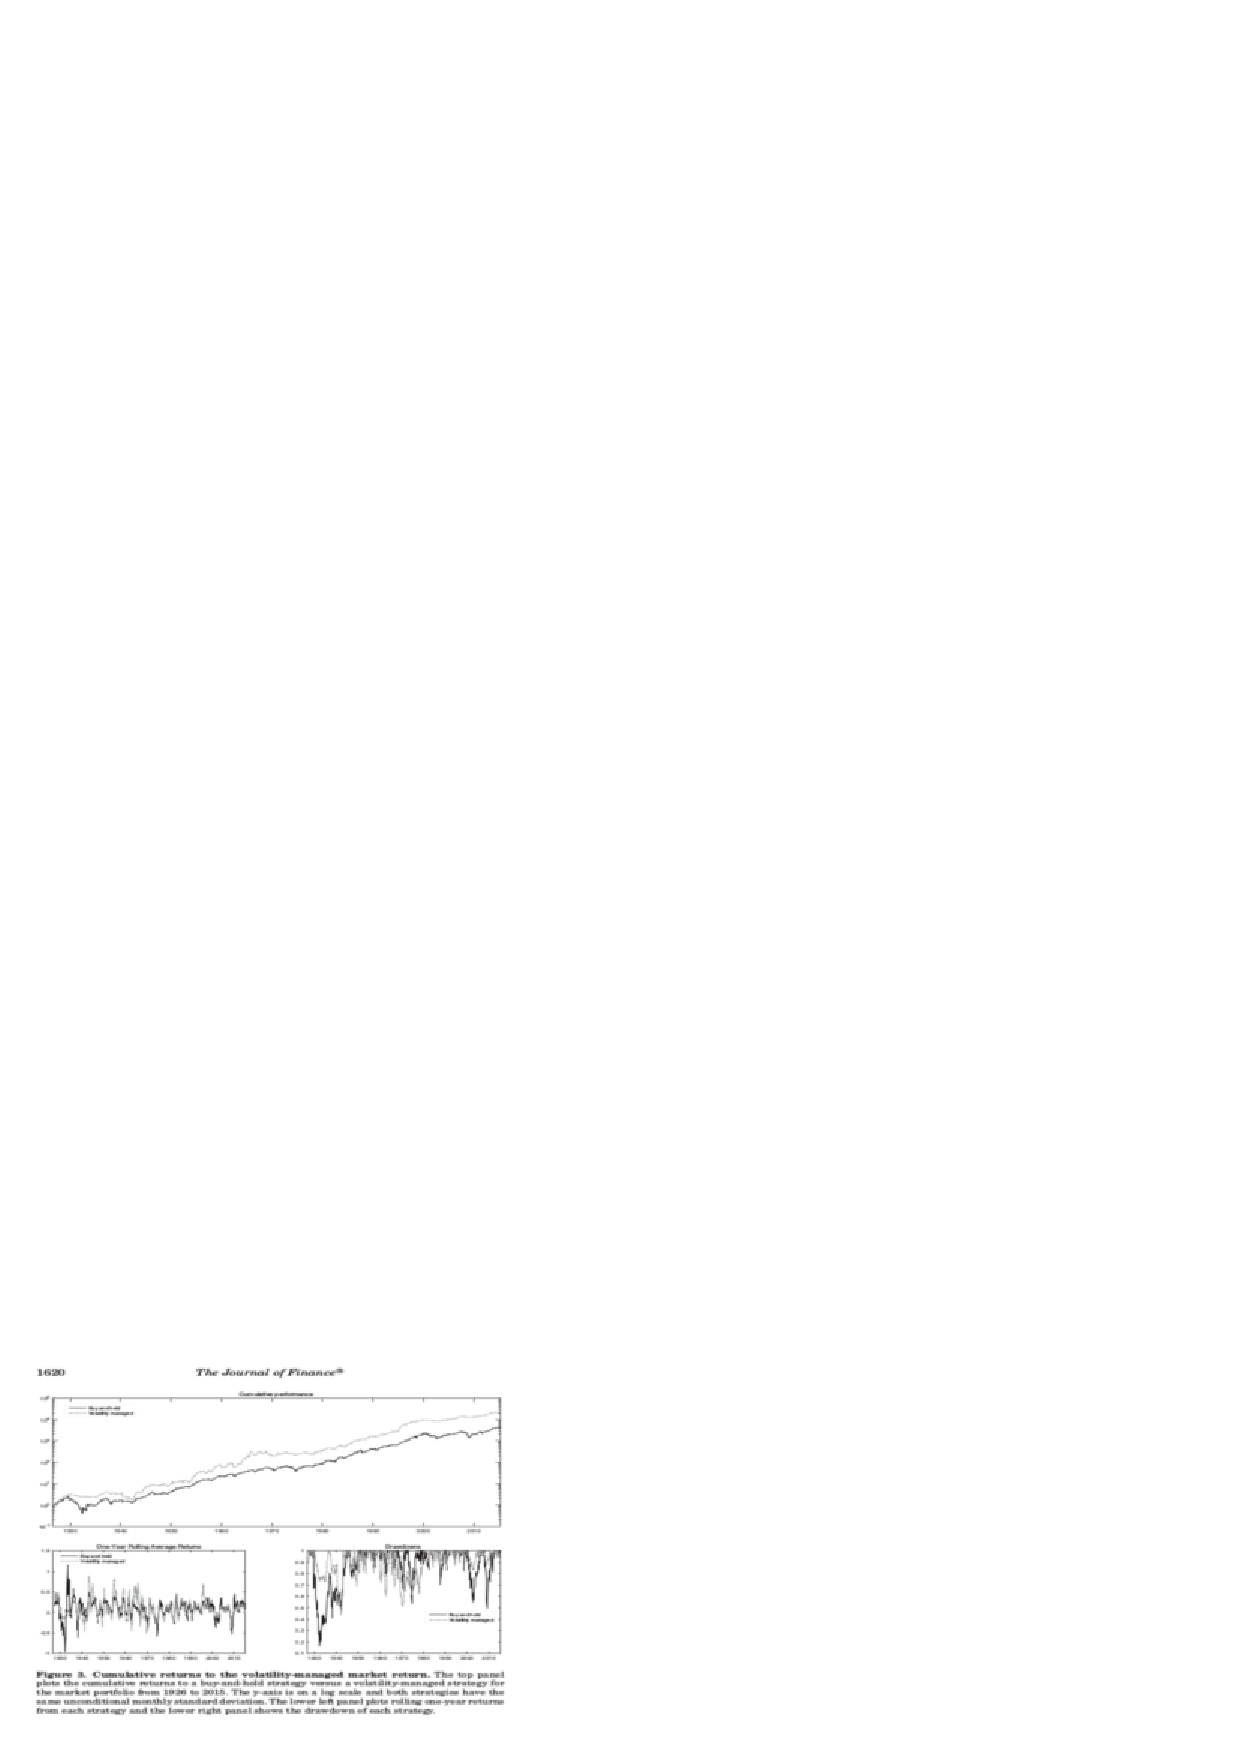
\includegraphics{mm}
	\end{figure}

\end{frame}

\begin{frame}{Variance Decomposition}
	\begin{itemize}[<+->]
	\item[]	%\begin{block}{Market Variance}
	Market Variance
			\begin{itemize}[<+->]
				\item Campbell, Lettau, and Xu (2001) - variance of individual assets vs market variance and CAPM
				\item Pollet and Wilson (2010) - decompose quarterly variance of market portfolio - Avg cor and Avg var
			\end{itemize}
	%	\end{block}
	\item[] Avg Var and Avg Cor
	%	\begin{block}{Avg Var and Avg Cor}

			\begin{align*}
			R_{s,t} &= \sum_{1}^{N}w_{n,t}R_{n,t} \\
			\sigma^{2}(r_{s,t}) &= \sum_{n=1}^{N} \sum_{m=1}^{N}w_{n,t}w_{m,t}\sigma^{2}_{n,t}\sigma^{2}_{m,t}\rho_{n,m,t}\\
			\sigma^{2}_{s,t} &= \sum_{n=1}^{N} w_{n,t}\sigma^{2}_{n,t} \times \sum_{n=1}^{N}\sum_{m \neq n}^{N}w_{n,t}w_{m,t}\rho_{n,m,t}\\
			AV_{t} &= \sum_{n=1}^{N} w_{n,t}\sigma^{2}_{n,t} ~ \text{ and } ~ AC_{t} = \sum_{n=1}^{N}\sum_{m \neq n}^{N}w_{n,t}w_{m,t}\rho_{n,m,t}
			\end{align*}
	%	\end{block}
	\end{itemize}
	
\end{frame}

\begin{frame}{Pollet and Wilson 2010 - Risk}
		\vspace{-12pt}
		\begin{table}
			\caption{1963Q2:2007Q1}
			\vspace{-18pt}
			\begin{adjustbox}{width=\textwidth,height=3cm}
				
% Table created by stargazer v.5.2 by Marek Hlavac, Harvard University. E-mail: hlavac at fas.harvard.edu
% Date and time: Mon, Mar 26, 2018 - 03:21:07  IST
\begin{tabular}{@{\extracolsep{5pt}}lccccc} 
\\[-1.8ex]\hline 
\hline \\[-1.8ex] 
\\[-1.8ex] & \multicolumn{5}{c}{SV$_{t+1}$} \\ 
\hline \\[-1.8ex] 
 AC$_{t}$ & 0.014$^{***}$ &  & 0.005 &  &  \\ 
 & (0.005) &  & (0.005) &  &  \\ 
 & & & & & \\ 
 AV$_{t}$ &  & 0.144$^{***}$ & 0.136$^{***}$ &  & 0.188$^{***}$ \\ 
 &  & (0.023) & (0.024) &  & (0.042) \\ 
 & & & & & \\ 
 SV$_{t}$ &  &  &  & 0.310$^{***}$ & $-$0.156 \\ 
 &  &  &  & (0.072) & (0.124) \\ 
 & & & & & \\ 
 Constant & 0.002 & 0.002$^{**}$ & 0.001 & 0.003$^{***}$ & 0.001$^{**}$ \\ 
 & (0.001) & (0.001) & (0.001) & (0.001) & (0.001) \\ 
 & & & & & \\ 
\hline \\[-1.8ex] 
Observations & 176 & 176 & 176 & 176 & 176 \\ 
R$^{2}$ & 0.042 & 0.184 & 0.096 & 0.096 & 0.191 \\ 
Adjusted R$^{2}$ & 0.037 & 0.179 & 0.091 & 0.091 & 0.182 \\ 
%Residual Std. Error & 0.006 (df = 174) & 0.006 (df = 174) & 0.006 (df = 174) & 0.006 (df = 174) & 0.006 (df = 173) \\ 
%F Statistic & 7.643$^{***}$ (df = 1; 174) & 39.124$^{***}$ (df = 1; 174) & 18.577$^{***}$ (df = 1; 174) & 18.577$^{***}$ (df = 1; 174) & 20.412$^{***}$ (df = 2; 173) \\ 
\hline 
\hline \\[-1.8ex] 
\textit{Note:}  & \multicolumn{5}{r}{$^{*}$p$<$0.1; $^{**}$p$<$0.05; $^{***}$p$<$0.01} \\ 
\end{tabular} 

			\end{adjustbox}
		\end{table}
\end{frame}

\begin{frame}{Pollet and Wilson 2010 - Returns}
		\vspace{-12pt}
		\begin{table}
			\caption{1963Q2:2007Q1}
			\vspace{-18pt}
			\begin{adjustbox}{width=\textwidth,height=3cm}
				
% Table created by stargazer v.5.2 by Marek Hlavac, Harvard University. E-mail: hlavac at fas.harvard.edu
% Date and time: Tue, Mar 13, 2018 - 07:14:38  IST
\begin{table}[!htbp] \centering 
  \caption{} 
  \label{} 
\begin{tabular}{@{\extracolsep{5pt}}lcccc} 
\\[-1.8ex]\hline 
\hline \\[-1.8ex] 
 & \multicolumn{4}{c}{\textit{Dependent variable:}} \\ 
\cline{2-5} 
\\[-1.8ex] & \multicolumn{4}{c}{RET$_{t+1}} \\ 
\\[-1.8ex] & (1) & (2) & (3) & (4)\\ 
\hline \\[-1.8ex] 
 AC$_{t}$ & 0.213$^{***}$ &  &  &  \\ 
  & (0.069) &  &  &  \\ 
  & & & & \\ 
 AV$_{t}$ &  & $-$0.117 &  & $-$1.742$^{***}$ \\ 
  &  & (0.347) &  & (0.616) \\ 
  & & & & \\ 
 SV$_{t}$ &  &  & 1.454 & 5.778$^{***}$ \\ 
  &  &  & (1.025) & (1.829) \\ 
  & & & & \\ 
 Constant & $-$0.037$^{**}$ & 0.014 & 0.005 & 0.022$^{**}$ \\ 
  & (0.017) & (0.010) & (0.008) & (0.010) \\ 
  & & & & \\ 
\hline \\[-1.8ex] 
Observations & 176 & 176 & 176 & 176 \\ 
R$^{2}$ & 0.053 & 0.001 & 0.011 & 0.055 \\ 
Adjusted R$^{2}$ & 0.047 & $-$0.005 & 0.006 & 0.044 \\ 
Residual Std. Error & 0.082 (df = 174) & 0.084 (df = 174) & 0.083 (df = 174) & 0.082 (df = 173) \\ 
F Statistic & 9.649$^{***}$ (df = 1; 174) & 0.113 (df = 1; 174) & 2.013 (df = 1; 174) & 5.049$^{***}$ (df = 2; 173) \\ 
\hline 
\hline \\[-1.8ex] 
\textit{Note:}  & \multicolumn{4}{r}{$^{*}$p$<$0.1; $^{**}$p$<$0.05; $^{***}$p$<$0.01} \\ 
\end{tabular} 
\end{table} 

			\end{adjustbox}
		\end{table}
\end{frame}

\begin{frame}{Average Variance}
	\begin{itemize}[<+->]
		\item Timing leverage by variance generates higher returns
		\item Market variance contains average correlation
		\item Average variance is at least unrelated to future returns
		\item $W_{t}$ = $\frac{1}{AV_{t-1}}$ is the investment weight on the CRSP market portfolio
		\item 	\begin{adjustbox}{width=\textwidth}
			% Created by tikzDevice version 0.10.1 on 2018-03-26 14:40:36
% !TEX encoding = UTF-8 Unicode
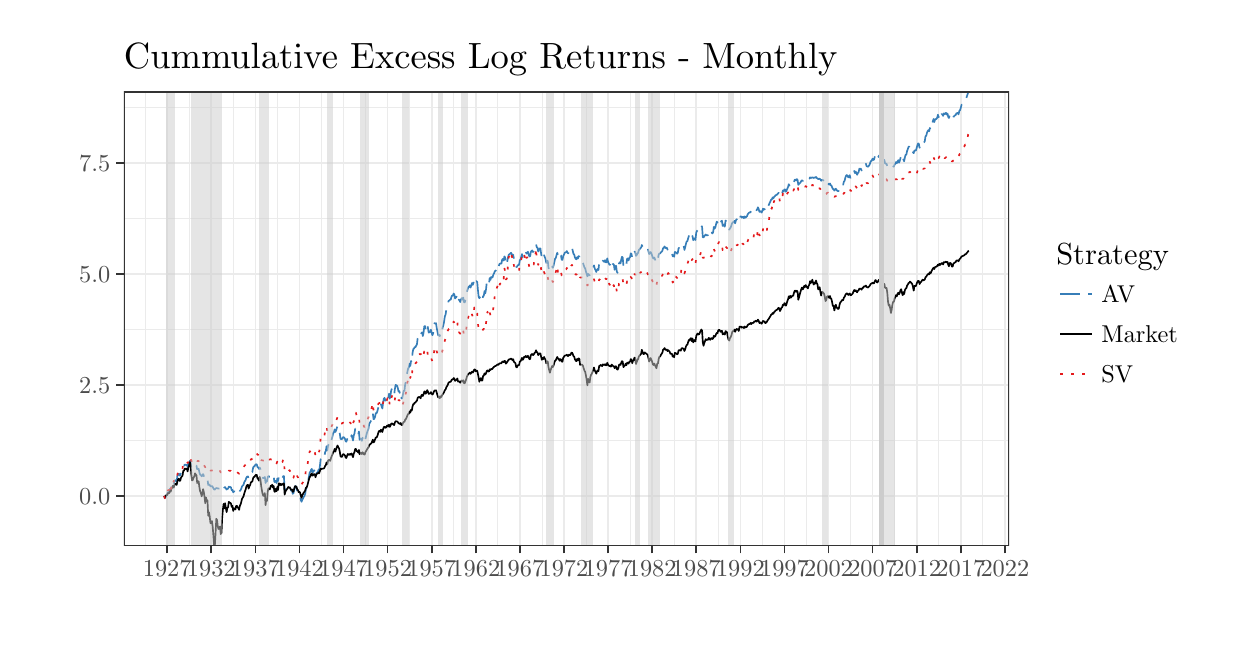
\begin{tikzpicture}[x=1pt,y=1pt]
\definecolor{fillColor}{RGB}{255,255,255}
\path[use as bounding box,fill=fillColor,fill opacity=0.00] (0,0) rectangle (426.79,216.81);
\begin{scope}
\path[clip] (  0.00,  0.00) rectangle (426.79,216.81);
\definecolor{drawColor}{RGB}{255,255,255}
\definecolor{fillColor}{RGB}{255,255,255}

\path[draw=drawColor,line width= 0.6pt,line join=round,line cap=round,fill=fillColor] (  0.00,  0.00) rectangle (426.79,216.81);
\end{scope}
\begin{scope}
\path[clip] ( 34.77, 29.59) rectangle (354.63,193.67);
\definecolor{fillColor}{RGB}{255,255,255}

\path[fill=fillColor] ( 34.77, 29.59) rectangle (354.63,193.67);
\definecolor{drawColor}{gray}{0.92}

\path[draw=drawColor,line width= 0.3pt,line join=round] ( 34.77, 67.61) --
	(354.63, 67.61);

\path[draw=drawColor,line width= 0.3pt,line join=round] ( 34.77,107.75) --
	(354.63,107.75);

\path[draw=drawColor,line width= 0.3pt,line join=round] ( 34.77,147.89) --
	(354.63,147.89);

\path[draw=drawColor,line width= 0.3pt,line join=round] ( 34.77,188.02) --
	(354.63,188.02);

\path[draw=drawColor,line width= 0.3pt,line join=round] ( 42.44, 29.59) --
	( 42.44,193.67);

\path[draw=drawColor,line width= 0.3pt,line join=round] ( 58.37, 29.59) --
	( 58.37,193.67);

\path[draw=drawColor,line width= 0.3pt,line join=round] ( 74.31, 29.59) --
	( 74.31,193.67);

\path[draw=drawColor,line width= 0.3pt,line join=round] ( 90.24, 29.59) --
	( 90.24,193.67);

\path[draw=drawColor,line width= 0.3pt,line join=round] (106.17, 29.59) --
	(106.17,193.67);

\path[draw=drawColor,line width= 0.3pt,line join=round] (122.10, 29.59) --
	(122.10,193.67);

\path[draw=drawColor,line width= 0.3pt,line join=round] (138.04, 29.59) --
	(138.04,193.67);

\path[draw=drawColor,line width= 0.3pt,line join=round] (153.97, 29.59) --
	(153.97,193.67);

\path[draw=drawColor,line width= 0.3pt,line join=round] (169.90, 29.59) --
	(169.90,193.67);

\path[draw=drawColor,line width= 0.3pt,line join=round] (185.83, 29.59) --
	(185.83,193.67);

\path[draw=drawColor,line width= 0.3pt,line join=round] (201.77, 29.59) --
	(201.77,193.67);

\path[draw=drawColor,line width= 0.3pt,line join=round] (217.70, 29.59) --
	(217.70,193.67);

\path[draw=drawColor,line width= 0.3pt,line join=round] (233.63, 29.59) --
	(233.63,193.67);

\path[draw=drawColor,line width= 0.3pt,line join=round] (249.57, 29.59) --
	(249.57,193.67);

\path[draw=drawColor,line width= 0.3pt,line join=round] (265.50, 29.59) --
	(265.50,193.67);

\path[draw=drawColor,line width= 0.3pt,line join=round] (281.44, 29.59) --
	(281.44,193.67);

\path[draw=drawColor,line width= 0.3pt,line join=round] (297.37, 29.59) --
	(297.37,193.67);

\path[draw=drawColor,line width= 0.3pt,line join=round] (313.30, 29.59) --
	(313.30,193.67);

\path[draw=drawColor,line width= 0.3pt,line join=round] (329.23, 29.59) --
	(329.23,193.67);

\path[draw=drawColor,line width= 0.3pt,line join=round] (345.17, 29.59) --
	(345.17,193.67);

\path[draw=drawColor,line width= 0.6pt,line join=round] ( 34.77, 47.54) --
	(354.63, 47.54);

\path[draw=drawColor,line width= 0.6pt,line join=round] ( 34.77, 87.68) --
	(354.63, 87.68);

\path[draw=drawColor,line width= 0.6pt,line join=round] ( 34.77,127.82) --
	(354.63,127.82);

\path[draw=drawColor,line width= 0.6pt,line join=round] ( 34.77,167.95) --
	(354.63,167.95);

\path[draw=drawColor,line width= 0.6pt,line join=round] ( 50.41, 29.59) --
	( 50.41,193.67);

\path[draw=drawColor,line width= 0.6pt,line join=round] ( 66.34, 29.59) --
	( 66.34,193.67);

\path[draw=drawColor,line width= 0.6pt,line join=round] ( 82.28, 29.59) --
	( 82.28,193.67);

\path[draw=drawColor,line width= 0.6pt,line join=round] ( 98.21, 29.59) --
	( 98.21,193.67);

\path[draw=drawColor,line width= 0.6pt,line join=round] (114.14, 29.59) --
	(114.14,193.67);

\path[draw=drawColor,line width= 0.6pt,line join=round] (130.07, 29.59) --
	(130.07,193.67);

\path[draw=drawColor,line width= 0.6pt,line join=round] (146.01, 29.59) --
	(146.01,193.67);

\path[draw=drawColor,line width= 0.6pt,line join=round] (161.94, 29.59) --
	(161.94,193.67);

\path[draw=drawColor,line width= 0.6pt,line join=round] (177.87, 29.59) --
	(177.87,193.67);

\path[draw=drawColor,line width= 0.6pt,line join=round] (193.80, 29.59) --
	(193.80,193.67);

\path[draw=drawColor,line width= 0.6pt,line join=round] (209.74, 29.59) --
	(209.74,193.67);

\path[draw=drawColor,line width= 0.6pt,line join=round] (225.67, 29.59) --
	(225.67,193.67);

\path[draw=drawColor,line width= 0.6pt,line join=round] (241.60, 29.59) --
	(241.60,193.67);

\path[draw=drawColor,line width= 0.6pt,line join=round] (257.53, 29.59) --
	(257.53,193.67);

\path[draw=drawColor,line width= 0.6pt,line join=round] (273.47, 29.59) --
	(273.47,193.67);

\path[draw=drawColor,line width= 0.6pt,line join=round] (289.40, 29.59) --
	(289.40,193.67);

\path[draw=drawColor,line width= 0.6pt,line join=round] (305.33, 29.59) --
	(305.33,193.67);

\path[draw=drawColor,line width= 0.6pt,line join=round] (321.26, 29.59) --
	(321.26,193.67);

\path[draw=drawColor,line width= 0.6pt,line join=round] (337.20, 29.59) --
	(337.20,193.67);

\path[draw=drawColor,line width= 0.6pt,line join=round] (353.13, 29.59) --
	(353.13,193.67);
\definecolor{drawColor}{RGB}{55,126,184}

\path[draw=drawColor,line width= 0.6pt,dash pattern=on 7pt off 3pt ,line join=round] ( 49.31, 47.61) --
	( 49.58, 46.82) --
	( 49.84, 47.22) --
	( 50.11, 47.85) --
	( 50.37, 47.83) --
	( 50.64, 48.93) --
	( 50.91, 48.96) --
	( 51.16, 49.05) --
	( 51.43, 50.24) --
	( 51.69, 49.70) --
	( 51.96, 51.16) --
	( 52.22, 51.62) --
	( 52.49, 52.47) --
	( 52.76, 51.59) --
	( 53.02, 52.85) --
	( 53.29, 53.30) --
	( 53.56, 53.18) --
	( 53.83, 52.79) --
	( 54.10, 54.88) --
	( 54.35, 55.42) --
	( 54.62, 55.62) --
	( 54.88, 55.00) --
	( 55.15, 55.05) --
	( 55.41, 56.24) --
	( 55.68, 56.69) --
	( 55.95, 56.95) --
	( 56.22, 58.52) --
	( 56.49, 58.53) --
	( 56.75, 58.89) --
	( 57.02, 58.88) --
	( 57.29, 58.74) --
	( 57.53, 58.87) --
	( 57.80, 58.09) --
	( 58.07, 58.97) --
	( 58.34, 59.42) --
	( 58.60, 60.28) --
	( 58.87, 59.80) --
	( 59.14, 57.72) --
	( 59.40, 57.59) --
	( 59.67, 57.61) --
	( 59.93, 57.83) --
	( 60.20, 58.08) --
	( 60.47, 58.99) --
	( 60.72, 58.73) --
	( 60.99, 58.52) --
	( 61.25, 57.25) --
	( 61.52, 57.41) --
	( 61.78, 57.42) --
	( 62.05, 56.09) --
	( 62.32, 55.27) --
	( 62.59, 55.15) --
	( 62.86, 54.71) --
	( 63.12, 54.98) --
	( 63.39, 55.50) --
	( 63.66, 54.82) --
	( 63.90, 54.13) --
	( 64.17, 53.56) --
	( 64.43, 54.02) --
	( 64.71, 53.84) --
	( 64.97, 53.86) --
	( 65.24, 51.55) --
	( 65.51, 51.74) --
	( 65.77, 51.62) --
	( 66.04, 51.07) --
	( 66.30, 51.05) --
	( 66.57, 51.17) --
	( 66.84, 50.91) --
	( 67.10, 50.40) --
	( 67.37, 49.92) --
	( 67.63, 49.91) --
	( 67.90, 50.28) --
	( 68.16, 50.45) --
	( 68.43, 50.41) --
	( 68.70, 50.30) --
	( 68.96, 50.23) --
	( 69.23, 50.34) --
	( 69.49, 50.36) --
	( 69.77, 49.49) --
	( 70.04, 49.61) --
	( 70.28, 50.13) --
	( 70.55, 50.50) --
	( 70.81, 50.85) --
	( 71.08, 50.60) --
	( 71.34, 50.80) --
	( 71.61, 50.28) --
	( 71.89, 49.92) --
	( 72.15, 50.15) --
	( 72.42, 50.24) --
	( 72.68, 50.96) --
	( 72.95, 50.81) --
	( 73.22, 50.84) --
	( 73.46, 50.69) --
	( 73.73, 49.63) --
	( 74.00, 49.80) --
	( 74.27, 48.93) --
	( 74.53, 49.21) --
	( 74.80, 49.20) --
	( 75.07, 49.04) --
	( 75.33, 49.68) --
	( 75.60, 49.71) --
	( 75.86, 49.39) --
	( 76.13, 49.14) --
	( 76.40, 48.71) --
	( 76.65, 49.37) --
	( 76.92, 49.70) --
	( 77.18, 50.21) --
	( 77.45, 51.01) --
	( 77.71, 51.36) --
	( 77.98, 51.58) --
	( 78.25, 52.52) --
	( 78.52, 52.96) --
	( 78.79, 53.46) --
	( 79.05, 54.26) --
	( 79.32, 54.56) --
	( 79.59, 54.67) --
	( 79.84, 53.85) --
	( 80.11, 54.34) --
	( 80.37, 54.65) --
	( 80.64, 55.89) --
	( 80.91, 56.08) --
	( 81.18, 56.28) --
	( 81.45, 57.75) --
	( 81.71, 58.28) --
	( 81.98, 58.31) --
	( 82.24, 58.84) --
	( 82.51, 59.05) --
	( 82.78, 59.00) --
	( 83.03, 58.02) --
	( 83.30, 57.95) --
	( 83.56, 57.38) --
	( 83.83, 57.85) --
	( 84.09, 57.29) --
	( 84.36, 54.72) --
	( 84.63, 54.33) --
	( 84.89, 54.18) --
	( 85.16, 54.07) --
	( 85.43, 54.12) --
	( 85.70, 54.46) --
	( 85.97, 52.29) --
	( 86.21, 52.98) --
	( 86.48, 52.83) --
	( 86.74, 54.36) --
	( 87.01, 54.76) --
	( 87.28, 54.55) --
	( 87.55, 54.58) --
	( 87.82, 54.88) --
	( 88.08, 54.71) --
	( 88.35, 55.18) --
	( 88.61, 54.50) --
	( 88.88, 54.77) --
	( 89.15, 52.65) --
	( 89.40, 52.63) --
	( 89.67, 53.05) --
	( 89.93, 52.27) --
	( 90.20, 53.89) --
	( 90.46, 52.98) --
	( 90.73, 54.29) --
	( 91.00, 54.27) --
	( 91.26, 53.56) --
	( 91.53, 54.28) --
	( 91.79, 53.74) --
	( 92.06, 54.09) --
	( 92.34, 54.76) --
	( 92.59, 54.78) --
	( 92.86, 49.55) --
	( 93.12, 49.76) --
	( 93.39, 49.94) --
	( 93.65, 50.40) --
	( 93.92, 50.70) --
	( 94.19, 51.10) --
	( 94.46, 50.78) --
	( 94.73, 50.84) --
	( 94.99, 49.74) --
	( 95.26, 49.45) --
	( 95.53, 49.62) --
	( 95.77, 48.37) --
	( 96.04, 48.60) --
	( 96.30, 49.72) --
	( 96.58, 51.12) --
	( 96.84, 51.09) --
	( 97.11, 50.84) --
	( 97.38, 49.41) --
	( 97.64, 48.95) --
	( 97.91, 47.86) --
	( 98.17, 47.92) --
	( 98.44, 47.61) --
	( 98.71, 46.10) --
	( 98.96, 45.49) --
	( 99.23, 46.26) --
	( 99.49, 46.66) --
	( 99.76, 47.29) --
	(100.02, 47.63) --
	(100.29, 48.39) --
	(100.56, 50.36) --
	(100.82, 50.37) --
	(101.09, 51.59) --
	(101.36, 53.07) --
	(101.63, 54.54) --
	(101.90, 56.12) --
	(102.14, 56.25) --
	(102.41, 57.06) --
	(102.67, 57.38) --
	(102.94, 56.15) --
	(103.21, 56.38) --
	(103.48, 56.88) --
	(103.75, 56.48) --
	(104.01, 54.54) --
	(104.28, 55.63) --
	(104.54, 56.03) --
	(104.81, 56.14) --
	(105.08, 57.05) --
	(105.33, 56.52) --
	(105.60, 58.48) --
	(105.87, 60.85) --
	(106.14, 60.42) --
	(106.40, 60.84) --
	(106.67, 60.85) --
	(106.94, 60.90) --
	(107.20, 61.62) --
	(107.47, 63.33) --
	(107.73, 63.89) --
	(108.00, 65.58) --
	(108.27, 64.04) --
	(108.52, 65.75) --
	(108.79, 66.26) --
	(109.05, 66.38) --
	(109.32, 65.82) --
	(109.58, 67.14) --
	(109.85, 68.06) --
	(110.12, 69.05) --
	(110.39, 70.30) --
	(110.66, 70.54) --
	(110.92, 71.62) --
	(111.19, 70.71) --
	(111.46, 71.32) --
	(111.70, 72.09) --
	(111.97, 72.94) --
	(112.24, 72.12) --
	(112.51, 71.54) --
	(112.77, 70.26) --
	(113.04, 68.22) --
	(113.31, 68.16) --
	(113.57, 68.16) --
	(113.84, 68.72) --
	(114.10, 68.86) --
	(114.37, 68.67) --
	(114.64, 68.26) --
	(114.89, 67.37) --
	(115.16, 67.19) --
	(115.42, 68.04) --
	(115.69, 68.86) --
	(115.95, 68.51) --
	(116.22, 68.37) --
	(116.49, 68.99) --
	(116.75, 68.47) --
	(117.03, 69.56) --
	(117.29, 68.68) --
	(117.56, 67.64) --
	(117.83, 69.45) --
	(118.08, 70.14) --
	(118.35, 71.88) --
	(118.61, 71.86) --
	(118.88, 70.54) --
	(119.15, 70.60) --
	(119.42, 69.67) --
	(119.69, 70.88) --
	(119.95, 67.88) --
	(120.22, 68.24) --
	(120.48, 68.31) --
	(120.75, 67.52) --
	(121.02, 68.61) --
	(121.27, 68.08) --
	(121.54, 66.92) --
	(121.80, 66.96) --
	(122.07, 68.24) --
	(122.33, 69.40) --
	(122.60, 70.41) --
	(122.87, 71.19) --
	(123.13, 71.83) --
	(123.40, 73.55) --
	(123.66, 74.07) --
	(123.93, 74.50) --
	(124.21, 75.03) --
	(124.45, 76.32) --
	(124.72, 77.55) --
	(124.98, 75.32) --
	(125.25, 75.49) --
	(125.51, 76.14) --
	(125.78, 77.49) --
	(126.05, 77.42) --
	(126.32, 78.09) --
	(126.59, 79.12) --
	(126.85, 80.02) --
	(127.12, 80.29) --
	(127.39, 79.45) --
	(127.63, 80.78) --
	(127.90, 79.97) --
	(128.17, 79.21) --
	(128.44, 81.48) --
	(128.70, 82.75) --
	(128.97, 83.03) --
	(129.24, 82.03) --
	(129.50, 82.14) --
	(129.77, 83.23) --
	(130.03, 83.94) --
	(130.30, 82.95) --
	(130.57, 84.51) --
	(130.83, 82.74) --
	(131.10, 83.94) --
	(131.36, 85.76) --
	(131.63, 86.38) --
	(131.89, 85.92) --
	(132.16, 84.50) --
	(132.43, 84.15) --
	(132.69, 86.28) --
	(132.96, 87.72) --
	(133.23, 87.58) --
	(133.50, 87.40) --
	(133.77, 86.53) --
	(134.01, 85.34) --
	(134.28, 85.51) --
	(134.54, 84.53) --
	(134.81, 85.32) --
	(135.08, 82.82) --
	(135.35, 82.90) --
	(135.62, 84.38) --
	(135.88, 85.66) --
	(136.15, 85.62) --
	(136.41, 87.98) --
	(136.68, 88.77) --
	(136.95, 90.64) --
	(137.20, 92.43) --
	(137.47, 93.63) --
	(137.73, 94.10) --
	(138.00, 95.41) --
	(138.26, 94.56) --
	(138.53, 96.38) --
	(138.80, 95.66) --
	(139.06, 99.20) --
	(139.33,100.66) --
	(139.60,100.84) --
	(139.87,101.41) --
	(140.14,101.34) --
	(140.38,101.92) --
	(140.65,102.33) --
	(140.91,104.48) --
	(141.18,105.12) --
	(141.44,105.19) --
	(141.72,105.09) --
	(141.99,104.76) --
	(142.25,106.36) --
	(142.52,106.71) --
	(142.78,105.37) --
	(143.05,106.61) --
	(143.32,108.90) --
	(143.57,109.00) --
	(143.84,107.55) --
	(144.11,108.36) --
	(144.38,109.51) --
	(144.64,108.29) --
	(144.91,106.60) --
	(145.18,106.82) --
	(145.44,106.90) --
	(145.71,107.69) --
	(145.97,106.48) --
	(146.24,105.69) --
	(146.51,106.36) --
	(146.76,108.65) --
	(147.03,110.06) --
	(147.29,109.80) --
	(147.56,110.02) --
	(147.82,108.19) --
	(148.09,106.84) --
	(148.36,105.63) --
	(148.62,105.86) --
	(148.90,105.34) --
	(149.16,106.50) --
	(149.43,106.04) --
	(149.70,107.23) --
	(149.94,108.43) --
	(150.21,109.29) --
	(150.47,110.57) --
	(150.74,112.51) --
	(151.01,113.13) --
	(151.28,115.01) --
	(151.55,116.03) --
	(151.81,116.80) --
	(152.08,118.04) --
	(152.34,118.22) --
	(152.61,118.49) --
	(152.88,118.57) --
	(153.13,119.56) --
	(153.40,120.03) --
	(153.66,119.99) --
	(153.93,120.73) --
	(154.19,120.33) --
	(154.46,118.96) --
	(154.73,119.26) --
	(154.99,119.67) --
	(155.26,120.36) --
	(155.53,118.20) --
	(155.80,118.55) --
	(156.07,118.14) --
	(156.32,117.68) --
	(156.59,118.58) --
	(156.85,119.07) --
	(157.12,118.54) --
	(157.38,119.27) --
	(157.65,117.65) --
	(157.92,117.51) --
	(158.19,118.54) --
	(158.46,119.87) --
	(158.72,121.42) --
	(158.99,122.27) --
	(159.26,123.10) --
	(159.50,123.20) --
	(159.77,123.67) --
	(160.04,122.87) --
	(160.31,123.75) --
	(160.57,124.54) --
	(160.84,123.89) --
	(161.11,124.65) --
	(161.37,125.95) --
	(161.64,125.92) --
	(161.90,124.75) --
	(162.17,125.21) --
	(162.44,124.92) --
	(162.69,122.08) --
	(162.96,119.51) --
	(163.22,119.06) --
	(163.49,119.57) --
	(163.75,119.96) --
	(164.02,118.43) --
	(164.29,118.43) --
	(164.56,119.74) --
	(164.83,119.98) --
	(165.09,121.63) --
	(165.36,120.81) --
	(165.63,122.33) --
	(165.87,124.63) --
	(166.14,125.34) --
	(166.40,124.42) --
	(166.68,124.21) --
	(166.94,126.34) --
	(167.21,125.66) --
	(167.48,126.71) --
	(167.74,126.47) --
	(168.01,126.71) --
	(168.27,127.59) --
	(168.54,128.06) --
	(168.81,128.82) --
	(169.07,128.91) --
	(169.34,129.44) --
	(169.60,129.96) --
	(169.87,130.66) --
	(170.13,129.98) --
	(170.40,131.26) --
	(170.67,131.56) --
	(170.93,131.57) --
	(171.20,131.61) --
	(171.47,133.04) --
	(171.74,133.24) --
	(172.01,132.66) --
	(172.25,134.17) --
	(172.52,133.76) --
	(172.78,131.04) --
	(173.05,131.35) --
	(173.31,132.45) --
	(173.59,133.87) --
	(173.86,134.84) --
	(174.12,134.84) --
	(174.39,135.22) --
	(174.65,135.45) --
	(174.92,135.07) --
	(175.19,134.28) --
	(175.43,134.74) --
	(175.71,133.22) --
	(175.97,133.01) --
	(176.24,132.59) --
	(176.50,130.41) --
	(176.77,130.29) --
	(177.04,130.88) --
	(177.30,131.04) --
	(177.57,131.08) --
	(177.83,132.84) --
	(178.10,132.99) --
	(178.37,134.11) --
	(178.62,134.98) --
	(178.89,133.89) --
	(179.15,134.44) --
	(179.42,135.35) --
	(179.68,135.15) --
	(179.95,136.00) --
	(180.22,135.18) --
	(180.49,135.29) --
	(180.76,135.85) --
	(181.02,134.85) --
	(181.29,134.14) --
	(181.56,134.17) --
	(181.81,135.77) --
	(182.08,136.14) --
	(182.34,136.30) --
	(182.61,135.74) --
	(182.88,136.02) --
	(183.15,137.13) --
	(183.42,137.26) --
	(183.68,138.63) --
	(183.95,137.52) --
	(184.21,137.25) --
	(184.48,135.93) --
	(184.75,136.64) --
	(185.00,137.05) --
	(185.27,137.06) --
	(185.53,135.14) --
	(185.80,133.51) --
	(186.06,134.14) --
	(186.33,133.59) --
	(186.60,134.57) --
	(186.86,133.90) --
	(187.13,133.22) --
	(187.40,131.81) --
	(187.67,132.62) --
	(187.94,132.45) --
	(188.18,130.14) --
	(188.45,128.96) --
	(188.71,128.63) --
	(188.98,129.33) --
	(189.25,129.86) --
	(189.52,130.44) --
	(189.79,130.04) --
	(190.05,130.89) --
	(190.32,132.17) --
	(190.58,133.33) --
	(190.85,133.62) --
	(191.12,134.70) --
	(191.37,135.47) --
	(191.64,134.49) --
	(191.90,134.50) --
	(192.17,133.49) --
	(192.43,134.62) --
	(192.70,134.49) --
	(192.97,132.99) --
	(193.23,132.86) --
	(193.50,134.26) --
	(193.76,134.73) --
	(194.03,135.43) --
	(194.31,135.60) --
	(194.56,135.67) --
	(194.83,136.09) --
	(195.09,135.48) --
	(195.36,135.26) --
	(195.62,136.06) --
	(195.89,135.84) --
	(196.16,136.02) --
	(196.43,137.09) --
	(196.70,137.26) --
	(196.96,136.20) --
	(197.23,135.05) --
	(197.50,134.82) --
	(197.74,133.79) --
	(198.01,133.28) --
	(198.27,133.12) --
	(198.55,133.88) --
	(198.81,133.38) --
	(199.08,134.25) --
	(199.35,134.13) --
	(199.61,132.21) --
	(199.88,132.25) --
	(200.14,132.25) --
	(200.41,132.21) --
	(200.68,131.76) --
	(200.93,130.92) --
	(201.20,130.15) --
	(201.46,129.79) --
	(201.73,128.67) --
	(201.99,127.90) --
	(202.26,126.93) --
	(202.53,127.81) --
	(202.79,127.59) --
	(203.06,127.31) --
	(203.33,128.46) --
	(203.60,128.84) --
	(203.87,129.12) --
	(204.11,129.64) --
	(204.38,130.25) --
	(204.64,130.90) --
	(204.91,129.74) --
	(205.18,129.20) --
	(205.45,128.54) --
	(205.72,129.27) --
	(205.98,129.65) --
	(206.25,129.24) --
	(206.51,131.67) --
	(206.78,131.71) --
	(207.05,132.14) --
	(207.30,131.87) --
	(207.58,131.54) --
	(207.84,132.62) --
	(208.11,132.37) --
	(208.37,132.18) --
	(208.64,132.79) --
	(208.91,132.00) --
	(209.17,132.03) --
	(209.44,133.45) --
	(209.70,132.24) --
	(209.97,131.63) --
	(210.24,131.13) --
	(210.49,131.18) --
	(210.76,130.75) --
	(211.02,132.52) --
	(211.29,131.89) --
	(211.55,131.30) --
	(211.82,131.21) --
	(212.09,129.32) --
	(212.36,130.63) --
	(212.63,130.72) --
	(212.89,128.64) --
	(213.16,128.20) --
	(213.43,129.31) --
	(213.67,131.61) --
	(213.94,132.02) --
	(214.21,131.64) --
	(214.48,132.97) --
	(214.74,134.01) --
	(215.01,133.75) --
	(215.28,130.67) --
	(215.54,131.17) --
	(215.81,131.33) --
	(216.07,132.25) --
	(216.34,131.39) --
	(216.61,133.35) --
	(216.86,133.39) --
	(217.13,132.70) --
	(217.39,133.63) --
	(217.66,133.81) --
	(217.92,135.24) --
	(218.19,135.07) --
	(218.46,133.48) --
	(218.72,134.18) --
	(219.00,134.53) --
	(219.26,135.85) --
	(219.53,135.76) --
	(219.80,134.34) --
	(220.05,134.63) --
	(220.32,135.11) --
	(220.58,135.48) --
	(220.85,136.47) --
	(221.12,136.75) --
	(221.39,137.14) --
	(221.66,137.29) --
	(221.92,138.27) --
	(222.19,137.71) --
	(222.45,137.21) --
	(222.72,137.24) --
	(222.99,137.78) --
	(223.24,137.54) --
	(223.51,137.56) --
	(223.77,137.25) --
	(224.04,137.09) --
	(224.30,136.06) --
	(224.57,134.99) --
	(224.84,135.42) --
	(225.10,135.72) --
	(225.37,135.25) --
	(225.63,134.49) --
	(225.90,133.69) --
	(226.18,133.39) --
	(226.42,133.75) --
	(226.69,133.11) --
	(226.95,132.31) --
	(227.22,131.87) --
	(227.48,133.38) --
	(227.75,133.42) --
	(228.02,134.88) --
	(228.29,135.18) --
	(228.56,135.26) --
	(228.82,135.62) --
	(229.09,135.84) --
	(229.36,136.24) --
	(229.60,137.13) --
	(229.87,137.25) --
	(230.14,137.75) --
	(230.41,137.23) --
	(230.67,137.18) --
	(230.94,137.31) --
	(231.21,136.62) --
	(231.47,136.97) --
	(231.74,136.62) --
	(232.00,136.19) --
	(232.27,135.37) --
	(232.54,135.44) --
	(232.80,135.37) --
	(233.07,134.20) --
	(233.33,134.48) --
	(233.60,134.02) --
	(233.86,135.75) --
	(234.13,135.66) --
	(234.40,135.47) --
	(234.66,135.13) --
	(234.93,135.48) --
	(235.20,137.09) --
	(235.47,137.28) --
	(235.74,137.08) --
	(235.98,136.91) --
	(236.25,138.19) --
	(236.51,138.41) --
	(236.78,138.23) --
	(237.05,138.00) --
	(237.32,136.49) --
	(237.59,137.49) --
	(237.85,138.63) --
	(238.12,139.59) --
	(238.38,139.66) --
	(238.65,140.65) --
	(238.92,141.54) --
	(239.17,141.32) --
	(239.44,141.91) --
	(239.70,142.08) --
	(239.97,140.79) --
	(240.23,141.55) --
	(240.50,140.00) --
	(240.77,140.48) --
	(241.03,140.67) --
	(241.30,140.09) --
	(241.57,142.71) --
	(241.84,143.33) --
	(242.11,143.67) --
	(242.35,143.33) --
	(242.62,143.34) --
	(242.88,143.84) --
	(243.15,144.66) --
	(243.41,145.30) --
	(243.69,144.86) --
	(243.96,141.10) --
	(244.22,141.01) --
	(244.49,141.46) --
	(244.75,141.76) --
	(245.02,142.07) --
	(245.29,141.74) --
	(245.54,141.84) --
	(245.81,141.78) --
	(246.08,142.64) --
	(246.35,142.41) --
	(246.61,141.64) --
	(246.88,142.44) --
	(247.15,142.75) --
	(247.41,142.45) --
	(247.68,142.84) --
	(247.94,144.82) --
	(248.21,144.20) --
	(248.48,144.66) --
	(248.73,145.69) --
	(249.00,146.72) --
	(249.26,146.40) --
	(249.53,147.64) --
	(249.79,148.02) --
	(250.06,147.84) --
	(250.33,146.66) --
	(250.59,146.77) --
	(250.87,147.06) --
	(251.13,145.15) --
	(251.40,145.28) --
	(251.67,145.73) --
	(251.91,144.89) --
	(252.18,147.13) --
	(252.44,146.86) --
	(252.71,146.48) --
	(252.98,144.61) --
	(253.25,144.11) --
	(253.52,143.84) --
	(253.78,144.32) --
	(254.05,144.63) --
	(254.31,145.45) --
	(254.58,146.22) --
	(254.85,146.52) --
	(255.10,146.49) --
	(255.37,147.01) --
	(255.63,146.11) --
	(255.90,147.12) --
	(256.16,147.59) --
	(256.43,147.31) --
	(256.70,147.66) --
	(256.96,146.92) --
	(257.23,148.61) --
	(257.50,148.53) --
	(257.77,148.65) --
	(258.04,148.15) --
	(258.29,148.42) --
	(258.56,148.47) --
	(258.82,147.94) --
	(259.09,148.63) --
	(259.35,148.14) --
	(259.62,148.42) --
	(259.89,148.61) --
	(260.16,149.33) --
	(260.43,149.70) --
	(260.69,149.94) --
	(260.96,149.99) --
	(261.23,150.32) --
	(261.47,149.81) --
	(261.74,150.14) --
	(262.01,150.20) --
	(262.28,150.14) --
	(262.54,150.91) --
	(262.81,150.87) --
	(263.08,151.19) --
	(263.34,150.84) --
	(263.61,151.15) --
	(263.87,151.89) --
	(264.14,151.34) --
	(264.41,150.27) --
	(264.66,150.40) --
	(264.93,150.49) --
	(265.19,149.98) --
	(265.46,150.52) --
	(265.72,151.44) --
	(265.99,151.00) --
	(266.26,151.28) --
	(266.53,150.39) --
	(266.80,150.58) --
	(267.06,150.95) --
	(267.33,151.75) --
	(267.60,152.39) --
	(267.84,152.86) --
	(268.11,153.51) --
	(268.38,154.01) --
	(268.65,154.69) --
	(268.91,154.76) --
	(269.18,155.47) --
	(269.45,155.13) --
	(269.71,155.68) --
	(269.98,155.85) --
	(270.24,156.24) --
	(270.51,156.37) --
	(270.78,156.48) --
	(271.04,156.76) --
	(271.31,157.12) --
	(271.57,156.88) --
	(271.84,155.55) --
	(272.10,155.86) --
	(272.37,156.75) --
	(272.64,156.95) --
	(272.90,157.98) --
	(273.17,157.67) --
	(273.44,158.39) --
	(273.71,158.31) --
	(273.98,157.52) --
	(274.22,158.00) --
	(274.49,158.64) --
	(274.75,159.21) --
	(275.02,160.24) --
	(275.28,159.76) --
	(275.56,160.49) --
	(275.83,159.96) --
	(276.09,160.11) --
	(276.36,160.29) --
	(276.62,160.30) --
	(276.89,161.01) --
	(277.16,161.83) --
	(277.40,161.93) --
	(277.68,161.62) --
	(277.94,162.08) --
	(278.21,161.75) --
	(278.47,160.00) --
	(278.74,160.34) --
	(279.01,160.63) --
	(279.27,160.86) --
	(279.54,161.43) --
	(279.80,161.69) --
	(280.07,161.43) --
	(280.34,161.69) --
	(280.59,162.01) --
	(280.86,161.90) --
	(281.12,162.22) --
	(281.39,161.97) --
	(281.65,161.83) --
	(281.92,161.61) --
	(282.19,162.07) --
	(282.46,162.24) --
	(282.73,162.70) --
	(282.99,162.49) --
	(283.26,162.57) --
	(283.53,162.76) --
	(283.78,162.59) --
	(284.05,162.50) --
	(284.31,162.67) --
	(284.58,162.57) --
	(284.85,162.87) --
	(285.12,162.51) --
	(285.39,162.36) --
	(285.65,162.10) --
	(285.92,162.15) --
	(286.18,162.25) --
	(286.45,161.98) --
	(286.72,161.49) --
	(286.97,161.78) --
	(287.24,161.80) --
	(287.50,161.62) --
	(287.77,161.41) --
	(288.03,160.93) --
	(288.30,159.80) --
	(288.57,159.93) --
	(288.83,160.36) --
	(289.10,160.53) --
	(289.37,160.32) --
	(289.64,160.08) --
	(289.91,160.52) --
	(290.15,159.89) --
	(290.42,159.77) --
	(290.68,159.17) --
	(290.95,158.48) --
	(291.22,158.50) --
	(291.49,157.92) --
	(291.76,158.40) --
	(292.02,158.61) --
	(292.29,158.19) --
	(292.55,157.86) --
	(292.82,157.71) --
	(293.09,157.86) --
	(293.34,158.58) --
	(293.61,159.38) --
	(293.87,159.60) --
	(294.14,159.96) --
	(294.40,160.33) --
	(294.67,160.08) --
	(294.94,161.19) --
	(295.20,161.48) --
	(295.47,162.65) --
	(295.73,163.28) --
	(296.00,163.55) --
	(296.28,163.24) --
	(296.53,162.72) --
	(296.80,162.97) --
	(297.06,163.49) --
	(297.33,162.29) --
	(297.59,162.33) --
	(297.86,162.80) --
	(298.13,163.24) --
	(298.40,164.15) --
	(298.67,165.04) --
	(298.93,164.24) --
	(299.20,164.80) --
	(299.47,164.29) --
	(299.71,163.63) --
	(299.98,164.28) --
	(300.25,164.56) --
	(300.52,165.86) --
	(300.78,165.63) --
	(301.05,165.87) --
	(301.32,165.21) --
	(301.58,165.78) --
	(301.85,165.80) --
	(302.11,167.02) --
	(302.38,166.92) --
	(302.65,167.34) --
	(302.90,167.60) --
	(303.17,166.72) --
	(303.43,166.65) --
	(303.70,166.55) --
	(303.96,166.91) --
	(304.23,167.30) --
	(304.50,168.17) --
	(304.76,168.64) --
	(305.03,168.82) --
	(305.30,169.47) --
	(305.57,168.99) --
	(305.84,169.22) --
	(306.08,170.14) --
	(306.35,171.21) --
	(306.61,170.66) --
	(306.88,169.70) --
	(307.15,169.83) --
	(307.42,170.16) --
	(307.69,170.64) --
	(307.95,169.90) --
	(308.22,169.84) --
	(308.48,168.79) --
	(308.75,168.62) --
	(309.02,168.49) --
	(309.27,168.80) --
	(309.55,169.01) --
	(309.81,167.81) --
	(310.08,167.64) --
	(310.34,167.68) --
	(310.61,166.76) --
	(310.88,166.32) --
	(311.14,166.23) --
	(311.41,166.26) --
	(311.67,166.04) --
	(311.94,165.70) --
	(312.21,166.08) --
	(312.46,166.33) --
	(312.73,166.60) --
	(312.99,166.58) --
	(313.26,167.35) --
	(313.52,167.65) --
	(313.79,168.25) --
	(314.06,167.82) --
	(314.33,168.40) --
	(314.60,168.93) --
	(314.86,168.03) --
	(315.13,168.63) --
	(315.40,169.77) --
	(315.64,170.39) --
	(315.91,168.90) --
	(316.18,168.47) --
	(316.45,169.18) --
	(316.71,168.53) --
	(316.98,170.00) --
	(317.25,170.84) --
	(317.51,170.95) --
	(317.78,172.29) --
	(318.04,172.93) --
	(318.31,173.79) --
	(318.58,173.87) --
	(318.83,174.39) --
	(319.10,173.95) --
	(319.36,173.45) --
	(319.63,173.00) --
	(319.89,171.81) --
	(320.16,171.46) --
	(320.43,172.43) --
	(320.69,172.38) --
	(320.97,172.42) --
	(321.23,173.34) --
	(321.50,174.29) --
	(321.77,174.99) --
	(322.02,174.81) --
	(322.29,173.41) --
	(322.55,174.20) --
	(322.82,174.36) --
	(323.09,174.86) --
	(323.36,175.73) --
	(323.63,175.27) --
	(323.89,175.43) --
	(324.16,175.71) --
	(324.42,177.56) --
	(324.69,177.77) --
	(324.96,178.79) --
	(325.21,179.43) --
	(325.48,179.78) --
	(325.74,179.39) --
	(326.01,180.55) --
	(326.27,179.91) --
	(326.54,180.99) --
	(326.81,182.34) --
	(327.07,182.91) --
	(327.34,183.82) --
	(327.60,182.69) --
	(327.88,183.65) --
	(328.15,183.78) --
	(328.39,183.83) --
	(328.66,184.27) --
	(328.92,185.35) --
	(329.19,184.42) --
	(329.45,185.59) --
	(329.72,184.49) --
	(330.00,185.29) --
	(330.26,185.60) --
	(330.53,185.47) --
	(330.79,184.92) --
	(331.06,185.85) --
	(331.33,185.56) --
	(331.57,185.75) --
	(331.84,186.04) --
	(332.11,185.37) --
	(332.38,185.79) --
	(332.64,184.55) --
	(332.91,184.17) --
	(333.18,185.18) --
	(333.44,185.22) --
	(333.71,184.71) --
	(333.97,183.75) --
	(334.24,183.75) --
	(334.51,184.55) --
	(334.77,184.82) --
	(335.04,185.13) --
	(335.30,185.21) --
	(335.57,185.82) --
	(335.83,185.91) --
	(336.10,186.03) --
	(336.37,185.46) --
	(336.63,186.69) --
	(336.90,186.99) --
	(337.17,187.80) --
	(337.44,188.93) --
	(337.71,189.00) --
	(337.95,189.39) --
	(338.22,189.85) --
	(338.48,190.17) --
	(338.75,190.84) --
	(339.02,190.88) --
	(339.29,191.72) --
	(339.56,192.54) --
	(339.82,193.33) --
	(340.09,193.67);
\definecolor{drawColor}{RGB}{0,0,0}

\path[draw=drawColor,line width= 0.6pt,line join=round] ( 49.31, 47.60) --
	( 49.58, 47.09) --
	( 49.84, 47.50) --
	( 50.11, 47.91) --
	( 50.37, 47.90) --
	( 50.64, 48.57) --
	( 50.91, 48.59) --
	( 51.16, 48.66) --
	( 51.43, 49.52) --
	( 51.69, 49.14) --
	( 51.96, 50.25) --
	( 52.22, 50.57) --
	( 52.49, 51.30) --
	( 52.76, 50.59) --
	( 53.02, 51.62) --
	( 53.29, 51.96) --
	( 53.56, 51.87) --
	( 53.83, 51.60) --
	( 54.10, 52.95) --
	( 54.35, 53.59) --
	( 54.62, 53.82) --
	( 54.88, 53.04) --
	( 55.15, 53.14) --
	( 55.41, 54.18) --
	( 55.68, 54.63) --
	( 55.95, 54.88) --
	( 56.22, 56.68) --
	( 56.49, 56.70) --
	( 56.75, 57.49) --
	( 57.02, 57.47) --
	( 57.29, 57.29) --
	( 57.53, 57.50) --
	( 57.80, 56.46) --
	( 58.07, 57.95) --
	( 58.34, 58.60) --
	( 58.60, 59.83) --
	( 58.87, 58.95) --
	( 59.14, 55.37) --
	( 59.40, 53.19) --
	( 59.67, 53.38) --
	( 59.93, 54.23) --
	( 60.20, 54.62) --
	( 60.47, 55.75) --
	( 60.72, 55.37) --
	( 60.99, 55.09) --
	( 61.25, 52.26) --
	( 61.52, 52.87) --
	( 61.78, 52.89) --
	( 62.05, 50.72) --
	( 62.32, 49.25) --
	( 62.59, 48.76) --
	( 62.86, 47.44) --
	( 63.12, 48.42) --
	( 63.39, 50.06) --
	( 63.66, 49.00) --
	( 63.90, 47.30) --
	( 64.17, 44.97) --
	( 64.43, 47.06) --
	( 64.71, 45.95) --
	( 64.97, 45.98) --
	( 65.24, 40.43) --
	( 65.51, 41.69) --
	( 65.77, 40.20) --
	( 66.04, 37.85) --
	( 66.30, 37.66) --
	( 66.57, 38.54) --
	( 66.84, 36.62) --
	( 67.10, 33.41) --
	( 67.37, 29.67) --
	( 67.63, 29.59) --
	( 67.90, 34.28) --
	( 68.16, 39.35) --
	( 68.43, 38.88) --
	( 68.70, 36.59) --
	( 68.96, 35.62) --
	( 69.23, 36.33) --
	( 69.49, 36.48) --
	( 69.77, 33.81) --
	( 70.04, 34.33) --
	( 70.28, 39.67) --
	( 70.55, 42.77) --
	( 70.81, 44.76) --
	( 71.08, 43.13) --
	( 71.34, 44.97) --
	( 71.61, 43.17) --
	( 71.89, 41.76) --
	( 72.15, 43.28) --
	( 72.42, 43.57) --
	( 72.68, 45.48) --
	( 72.95, 45.08) --
	( 73.22, 45.15) --
	( 73.46, 44.85) --
	( 73.73, 43.64) --
	( 74.00, 44.04) --
	( 74.27, 42.18) --
	( 74.53, 43.07) --
	( 74.80, 43.03) --
	( 75.07, 42.72) --
	( 75.33, 43.98) --
	( 75.60, 44.04) --
	( 75.86, 43.49) --
	( 76.13, 43.17) --
	( 76.40, 42.58) --
	( 76.65, 43.97) --
	( 76.92, 44.51) --
	( 77.18, 45.42) --
	( 77.45, 46.56) --
	( 77.71, 46.98) --
	( 77.98, 47.40) --
	( 78.25, 48.47) --
	( 78.52, 49.30) --
	( 78.79, 50.03) --
	( 79.05, 51.11) --
	( 79.32, 51.51) --
	( 79.59, 51.64) --
	( 79.84, 50.27) --
	( 80.11, 51.09) --
	( 80.37, 51.47) --
	( 80.64, 52.50) --
	( 80.91, 52.67) --
	( 81.18, 52.85) --
	( 81.45, 53.94) --
	( 81.71, 54.45) --
	( 81.98, 54.50) --
	( 82.24, 55.02) --
	( 82.51, 55.23) --
	( 82.78, 55.18) --
	( 83.03, 53.92) --
	( 83.30, 53.81) --
	( 83.56, 53.12) --
	( 83.83, 54.49) --
	( 84.09, 53.69) --
	( 84.36, 51.32) --
	( 84.63, 49.70) --
	( 84.89, 48.30) --
	( 85.16, 47.63) --
	( 85.43, 47.74) --
	( 85.70, 48.64) --
	( 85.97, 44.27) --
	( 86.21, 46.46) --
	( 86.48, 45.82) --
	( 86.74, 49.25) --
	( 87.01, 50.36) --
	( 87.28, 49.92) --
	( 87.55, 50.07) --
	( 87.82, 51.28) --
	( 88.08, 50.99) --
	( 88.35, 51.64) --
	( 88.61, 50.65) --
	( 88.88, 51.21) --
	( 89.15, 49.15) --
	( 89.40, 49.11) --
	( 89.67, 50.19) --
	( 89.93, 49.30) --
	( 90.20, 50.86) --
	( 90.46, 49.74) --
	( 90.73, 52.15) --
	( 91.00, 52.08) --
	( 91.26, 51.48) --
	( 91.53, 51.95) --
	( 91.79, 51.55) --
	( 92.06, 51.79) --
	( 92.34, 52.08) --
	( 92.59, 52.10) --
	( 92.86, 48.09) --
	( 93.12, 49.12) --
	( 93.39, 49.63) --
	( 93.65, 50.02) --
	( 93.92, 50.38) --
	( 94.19, 50.86) --
	( 94.46, 50.59) --
	( 94.73, 50.70) --
	( 94.99, 50.02) --
	( 95.26, 49.80) --
	( 95.53, 49.95) --
	( 95.77, 49.06) --
	( 96.04, 49.27) --
	( 96.30, 50.18) --
	( 96.58, 51.11) --
	( 96.84, 51.09) --
	( 97.11, 50.96) --
	( 97.38, 50.09) --
	( 97.64, 49.76) --
	( 97.91, 48.99) --
	( 98.17, 49.14) --
	( 98.44, 48.75) --
	( 98.71, 47.66) --
	( 98.96, 46.95) --
	( 99.23, 47.88) --
	( 99.49, 48.29) --
	( 99.76, 48.84) --
	(100.02, 49.13) --
	(100.29, 49.56) --
	(100.56, 50.63) --
	(100.82, 50.64) --
	(101.09, 51.44) --
	(101.36, 52.57) --
	(101.63, 53.51) --
	(101.90, 54.47) --
	(102.14, 54.58) --
	(102.41, 55.47) --
	(102.67, 55.74) --
	(102.94, 54.95) --
	(103.21, 55.16) --
	(103.48, 55.53) --
	(103.75, 55.34) --
	(104.01, 54.34) --
	(104.28, 55.34) --
	(104.54, 55.62) --
	(104.81, 55.67) --
	(105.08, 56.06) --
	(105.33, 55.79) --
	(105.60, 56.58) --
	(105.87, 57.46) --
	(106.14, 57.21) --
	(106.40, 57.46) --
	(106.67, 57.46) --
	(106.94, 57.49) --
	(107.20, 57.75) --
	(107.47, 58.39) --
	(107.73, 58.71) --
	(108.00, 59.71) --
	(108.27, 59.06) --
	(108.52, 60.27) --
	(108.79, 60.56) --
	(109.05, 60.63) --
	(109.32, 60.26) --
	(109.58, 61.22) --
	(109.85, 61.97) --
	(110.12, 62.58) --
	(110.39, 63.43) --
	(110.66, 63.64) --
	(110.92, 64.62) --
	(111.19, 63.65) --
	(111.46, 64.55) --
	(111.70, 65.21) --
	(111.97, 65.84) --
	(112.24, 65.20) --
	(112.51, 64.77) --
	(112.77, 63.69) --
	(113.04, 61.96) --
	(113.31, 61.73) --
	(113.57, 61.73) --
	(113.84, 62.51) --
	(114.10, 62.72) --
	(114.37, 62.53) --
	(114.64, 62.26) --
	(114.89, 61.47) --
	(115.16, 61.31) --
	(115.42, 62.14) --
	(115.69, 62.78) --
	(115.95, 62.50) --
	(116.22, 62.42) --
	(116.49, 62.80) --
	(116.75, 62.49) --
	(117.03, 62.97) --
	(117.29, 62.34) --
	(117.56, 61.61) --
	(117.83, 62.87) --
	(118.08, 63.46) --
	(118.35, 64.60) --
	(118.61, 64.58) --
	(118.88, 63.74) --
	(119.15, 63.79) --
	(119.42, 63.29) --
	(119.69, 64.21) --
	(119.95, 62.66) --
	(120.22, 63.17) --
	(120.48, 63.21) --
	(120.75, 62.73) --
	(121.02, 63.37) --
	(121.27, 63.06) --
	(121.54, 62.58) --
	(121.80, 62.60) --
	(122.07, 63.47) --
	(122.33, 63.88) --
	(122.60, 64.37) --
	(122.87, 64.86) --
	(123.13, 65.14) --
	(123.40, 65.94) --
	(123.66, 66.21) --
	(123.93, 66.44) --
	(124.21, 66.63) --
	(124.45, 67.26) --
	(124.72, 67.93) --
	(124.98, 66.96) --
	(125.25, 67.20) --
	(125.51, 67.98) --
	(125.78, 68.73) --
	(126.05, 68.70) --
	(126.32, 69.14) --
	(126.59, 70.03) --
	(126.85, 70.93) --
	(127.12, 71.13) --
	(127.39, 70.77) --
	(127.63, 71.54) --
	(127.90, 71.16) --
	(128.17, 70.72) --
	(128.44, 71.81) --
	(128.70, 72.50) --
	(128.97, 72.62) --
	(129.24, 72.23) --
	(129.50, 72.31) --
	(129.77, 72.85) --
	(130.03, 73.10) --
	(130.30, 72.67) --
	(130.57, 73.37) --
	(130.83, 72.54) --
	(131.10, 73.04) --
	(131.36, 73.64) --
	(131.63, 73.80) --
	(131.89, 73.67) --
	(132.16, 73.34) --
	(132.43, 73.23) --
	(132.69, 74.13) --
	(132.96, 74.60) --
	(133.23, 74.55) --
	(133.50, 74.50) --
	(133.77, 74.27) --
	(134.01, 73.79) --
	(134.28, 73.87) --
	(134.54, 73.58) --
	(134.81, 73.95) --
	(135.08, 73.20) --
	(135.35, 73.23) --
	(135.62, 73.94) --
	(135.88, 74.37) --
	(136.15, 74.36) --
	(136.41, 75.17) --
	(136.68, 75.43) --
	(136.95, 76.00) --
	(137.20, 76.67) --
	(137.47, 77.16) --
	(137.73, 77.33) --
	(138.00, 78.11) --
	(138.26, 77.73) --
	(138.53, 78.73) --
	(138.80, 78.46) --
	(139.06, 79.91) --
	(139.33, 80.76) --
	(139.60, 80.86) --
	(139.87, 81.35) --
	(140.14, 81.32) --
	(140.38, 81.81) --
	(140.65, 81.99) --
	(140.91, 83.00) --
	(141.18, 83.30) --
	(141.44, 83.35) --
	(141.72, 83.30) --
	(141.99, 82.86) --
	(142.25, 83.95) --
	(142.52, 84.18) --
	(142.78, 83.70) --
	(143.05, 84.29) --
	(143.32, 85.32) --
	(143.57, 85.37) --
	(143.84, 84.54) --
	(144.11, 85.09) --
	(144.38, 85.85) --
	(144.64, 85.33) --
	(144.91, 84.48) --
	(145.18, 84.57) --
	(145.44, 84.62) --
	(145.71, 85.13) --
	(145.97, 84.57) --
	(146.24, 84.23) --
	(146.51, 84.57) --
	(146.76, 85.24) --
	(147.03, 85.78) --
	(147.29, 85.66) --
	(147.56, 85.76) --
	(147.82, 84.90) --
	(148.09, 83.90) --
	(148.36, 83.18) --
	(148.62, 83.55) --
	(148.90, 82.89) --
	(149.16, 83.62) --
	(149.43, 83.35) --
	(149.70, 83.84) --
	(149.94, 84.31) --
	(150.21, 84.68) --
	(150.47, 85.14) --
	(150.74, 85.82) --
	(151.01, 86.12) --
	(151.28, 86.87) --
	(151.55, 87.30) --
	(151.81, 87.75) --
	(152.08, 88.55) --
	(152.34, 88.68) --
	(152.61, 88.83) --
	(152.88, 88.87) --
	(153.13, 89.43) --
	(153.40, 89.71) --
	(153.66, 89.69) --
	(153.93, 90.20) --
	(154.19, 89.96) --
	(154.46, 89.18) --
	(154.73, 89.40) --
	(154.99, 89.64) --
	(155.26, 90.04) --
	(155.53, 88.90) --
	(155.80, 89.07) --
	(156.07, 88.81) --
	(156.32, 88.52) --
	(156.59, 89.00) --
	(156.85, 89.33) --
	(157.12, 88.92) --
	(157.38, 89.39) --
	(157.65, 88.40) --
	(157.92, 88.30) --
	(158.19, 89.03) --
	(158.46, 89.76) --
	(158.72, 90.73) --
	(158.99, 91.29) --
	(159.26, 91.74) --
	(159.50, 91.81) --
	(159.77, 92.19) --
	(160.04, 91.70) --
	(160.31, 92.14) --
	(160.57, 92.54) --
	(160.84, 92.18) --
	(161.11, 92.59) --
	(161.37, 93.28) --
	(161.64, 93.26) --
	(161.90, 92.65) --
	(162.17, 92.93) --
	(162.44, 92.81) --
	(162.69, 91.73) --
	(162.96, 90.28) --
	(163.22, 88.86) --
	(163.49, 89.84) --
	(163.75, 90.18) --
	(164.02, 89.31) --
	(164.29, 89.30) --
	(164.56, 90.95) --
	(164.83, 91.10) --
	(165.09, 91.88) --
	(165.36, 91.48) --
	(165.63, 91.96) --
	(165.87, 92.67) --
	(166.14, 92.95) --
	(166.40, 92.62) --
	(166.68, 92.55) --
	(166.94, 93.34) --
	(167.21, 93.11) --
	(167.48, 93.51) --
	(167.74, 93.37) --
	(168.01, 93.67) --
	(168.27, 94.04) --
	(168.54, 94.26) --
	(168.81, 94.50) --
	(169.07, 94.53) --
	(169.34, 94.76) --
	(169.60, 94.95) --
	(169.87, 95.23) --
	(170.13, 95.00) --
	(170.40, 95.43) --
	(170.67, 95.53) --
	(170.93, 95.53) --
	(171.20, 95.55) --
	(171.47, 96.11) --
	(171.74, 96.17) --
	(172.01, 95.97) --
	(172.25, 96.45) --
	(172.52, 96.32) --
	(172.78, 95.42) --
	(173.05, 95.64) --
	(173.31, 96.07) --
	(173.59, 96.52) --
	(173.86, 96.93) --
	(174.12, 96.93) --
	(174.39, 97.10) --
	(174.65, 97.24) --
	(174.92, 97.05) --
	(175.19, 96.64) --
	(175.43, 96.98) --
	(175.71, 96.06) --
	(175.97, 95.83) --
	(176.24, 95.56) --
	(176.50, 94.24) --
	(176.77, 94.07) --
	(177.04, 94.67) --
	(177.30, 94.89) --
	(177.57, 94.91) --
	(177.83, 96.17) --
	(178.10, 96.28) --
	(178.37, 96.89) --
	(178.62, 97.49) --
	(178.89, 96.78) --
	(179.15, 97.16) --
	(179.42, 97.88) --
	(179.68, 97.73) --
	(179.95, 98.22) --
	(180.22, 97.73) --
	(180.49, 97.80) --
	(180.76, 98.27) --
	(181.02, 97.62) --
	(181.29, 97.02) --
	(181.56, 97.03) --
	(181.81, 98.42) --
	(182.08, 98.78) --
	(182.34, 98.90) --
	(182.61, 98.47) --
	(182.88, 98.69) --
	(183.15, 99.31) --
	(183.42, 99.39) --
	(183.68,100.23) --
	(183.95, 99.61) --
	(184.21, 99.43) --
	(184.48, 98.48) --
	(184.75, 98.87) --
	(185.00, 99.13) --
	(185.27, 99.13) --
	(185.53, 97.93) --
	(185.80, 96.77) --
	(186.06, 97.50) --
	(186.33, 97.04) --
	(186.60, 97.83) --
	(186.86, 97.21) --
	(187.13, 96.79) --
	(187.40, 95.49) --
	(187.67, 96.27) --
	(187.94, 96.10) --
	(188.18, 94.21) --
	(188.45, 93.05) --
	(188.71, 92.13) --
	(188.98, 93.20) --
	(189.25, 93.89) --
	(189.52, 94.55) --
	(189.79, 94.17) --
	(190.05, 94.87) --
	(190.32, 95.75) --
	(190.58, 96.49) --
	(190.85, 96.69) --
	(191.12, 97.33) --
	(191.37, 97.81) --
	(191.64, 97.16) --
	(191.90, 97.17) --
	(192.17, 96.46) --
	(192.43, 97.07) --
	(192.70, 96.92) --
	(192.97, 96.18) --
	(193.23, 96.10) --
	(193.50, 97.45) --
	(193.76, 97.84) --
	(194.03, 98.27) --
	(194.31, 98.36) --
	(194.56, 98.41) --
	(194.83, 98.63) --
	(195.09, 98.24) --
	(195.36, 98.13) --
	(195.62, 98.65) --
	(195.89, 98.48) --
	(196.16, 98.57) --
	(196.43, 99.29) --
	(196.70, 99.41) --
	(196.96, 98.90) --
	(197.23, 98.11) --
	(197.50, 97.92) --
	(197.74, 97.00) --
	(198.01, 96.53) --
	(198.27, 96.30) --
	(198.55, 97.11) --
	(198.81, 96.55) --
	(199.08, 97.29) --
	(199.35, 97.17) --
	(199.61, 94.99) --
	(199.88, 95.07) --
	(200.14, 95.05) --
	(200.41, 94.99) --
	(200.68, 94.51) --
	(200.93, 93.66) --
	(201.20, 92.88) --
	(201.46, 92.39) --
	(201.73, 91.09) --
	(201.99, 89.52) --
	(202.26, 87.54) --
	(202.53, 89.90) --
	(202.79, 89.10) --
	(203.06, 88.58) --
	(203.33, 90.62) --
	(203.60, 91.42) --
	(203.87, 91.81) --
	(204.11, 92.47) --
	(204.38, 93.26) --
	(204.64, 94.00) --
	(204.91, 92.93) --
	(205.18, 92.48) --
	(205.45, 91.78) --
	(205.72, 92.58) --
	(205.98, 92.98) --
	(206.25, 92.72) --
	(206.51, 94.56) --
	(206.78, 94.60) --
	(207.05, 94.95) --
	(207.30, 94.72) --
	(207.58, 94.51) --
	(207.84, 95.14) --
	(208.11, 94.98) --
	(208.37, 94.89) --
	(208.64, 95.20) --
	(208.91, 94.80) --
	(209.17, 94.82) --
	(209.44, 95.71) --
	(209.70, 95.06) --
	(209.97, 94.74) --
	(210.24, 94.53) --
	(210.49, 94.55) --
	(210.76, 94.32) --
	(211.02, 95.06) --
	(211.29, 94.80) --
	(211.55, 94.52) --
	(211.82, 94.47) --
	(212.09, 93.76) --
	(212.36, 94.40) --
	(212.63, 94.46) --
	(212.89, 93.47) --
	(213.16, 93.24) --
	(213.43, 93.70) --
	(213.67, 94.90) --
	(213.94, 95.18) --
	(214.21, 94.92) --
	(214.48, 95.73) --
	(214.74, 96.31) --
	(215.01, 96.11) --
	(215.28, 94.13) --
	(215.54, 94.56) --
	(215.81, 94.74) --
	(216.07, 95.40) --
	(216.34, 94.84) --
	(216.61, 95.74) --
	(216.86, 95.76) --
	(217.13, 95.41) --
	(217.39, 96.01) --
	(217.66, 96.12) --
	(217.92, 97.00) --
	(218.19, 96.90) --
	(218.46, 95.56) --
	(218.72, 96.42) --
	(219.00, 96.73) --
	(219.26, 97.59) --
	(219.53, 97.46) --
	(219.80, 95.27) --
	(220.05, 95.95) --
	(220.32, 96.69) --
	(220.58, 97.08) --
	(220.85, 98.03) --
	(221.12, 98.31) --
	(221.39, 98.69) --
	(221.66, 98.91) --
	(221.92,100.39) --
	(222.19, 99.68) --
	(222.45, 98.87) --
	(222.72, 98.90) --
	(222.99, 99.46) --
	(223.24, 99.11) --
	(223.51, 99.13) --
	(223.77, 98.80) --
	(224.04, 98.56) --
	(224.30, 97.42) --
	(224.57, 96.16) --
	(224.84, 96.89) --
	(225.10, 97.42) --
	(225.37, 96.77) --
	(225.63, 96.17) --
	(225.90, 95.19) --
	(226.18, 94.90) --
	(226.42, 95.43) --
	(226.69, 94.81) --
	(226.95, 94.24) --
	(227.22, 93.74) --
	(227.48, 95.39) --
	(227.75, 95.49) --
	(228.02, 97.17) --
	(228.29, 97.90) --
	(228.56, 98.04) --
	(228.82, 98.60) --
	(229.09, 98.97) --
	(229.36, 99.40) --
	(229.60,100.45) --
	(229.87,100.56) --
	(230.14,101.05) --
	(230.41,100.42) --
	(230.67,100.37) --
	(230.94,100.51) --
	(231.21, 99.93) --
	(231.47,100.27) --
	(231.74, 99.98) --
	(232.00, 99.66) --
	(232.27, 98.91) --
	(232.54, 99.00) --
	(232.80, 98.92) --
	(233.07, 97.94) --
	(233.33, 98.19) --
	(233.60, 97.73) --
	(233.86, 99.32) --
	(234.13, 99.20) --
	(234.40, 99.06) --
	(234.66, 98.75) --
	(234.93, 98.97) --
	(235.20,100.17) --
	(235.47,100.34) --
	(235.74,100.21) --
	(235.98,100.08) --
	(236.25,100.85) --
	(236.51,101.01) --
	(236.78,100.90) --
	(237.05,100.73) --
	(237.32, 99.98) --
	(237.59,100.59) --
	(237.85,101.57) --
	(238.12,102.14) --
	(238.38,102.20) --
	(238.65,103.22) --
	(238.92,103.97) --
	(239.17,103.76) --
	(239.44,104.46) --
	(239.70,104.61) --
	(239.97,103.54) --
	(240.23,104.49) --
	(240.50,103.08) --
	(240.77,103.78) --
	(241.03,103.95) --
	(241.30,103.44) --
	(241.57,105.32) --
	(241.84,106.00) --
	(242.11,106.30) --
	(242.35,105.96) --
	(242.62,105.97) --
	(242.88,106.58) --
	(243.15,107.22) --
	(243.41,107.73) --
	(243.69,107.31) --
	(243.96,103.14) --
	(244.22,101.86) --
	(244.49,102.86) --
	(244.75,103.51) --
	(245.02,104.25) --
	(245.29,103.94) --
	(245.54,104.04) --
	(245.81,103.98) --
	(246.08,104.71) --
	(246.35,104.51) --
	(246.61,103.98) --
	(246.88,104.48) --
	(247.15,104.67) --
	(247.41,104.30) --
	(247.68,104.54) --
	(247.94,105.48) --
	(248.21,105.11) --
	(248.48,105.36) --
	(248.73,106.02) --
	(249.00,106.53) --
	(249.26,106.35) --
	(249.53,107.41) --
	(249.79,107.65) --
	(250.06,107.51) --
	(250.33,106.92) --
	(250.59,107.10) --
	(250.87,107.28) --
	(251.13,106.00) --
	(251.40,106.14) --
	(251.67,106.43) --
	(251.91,105.88) --
	(252.18,107.15) --
	(252.44,106.97) --
	(252.71,106.71) --
	(252.98,105.06) --
	(253.25,104.06) --
	(253.52,103.76) --
	(253.78,104.68) --
	(254.05,105.04) --
	(254.31,105.72) --
	(254.58,106.80) --
	(254.85,107.17) --
	(255.10,107.15) --
	(255.37,107.72) --
	(255.63,106.91) --
	(255.90,107.57) --
	(256.16,107.93) --
	(256.43,107.67) --
	(256.70,107.88) --
	(256.96,107.20) --
	(257.23,108.76) --
	(257.50,108.68) --
	(257.77,108.83) --
	(258.04,108.39) --
	(258.29,108.56) --
	(258.56,108.61) --
	(258.82,108.24) --
	(259.09,108.83) --
	(259.35,108.44) --
	(259.62,108.59) --
	(259.89,108.72) --
	(260.16,109.31) --
	(260.43,109.56) --
	(260.69,109.72) --
	(260.96,109.76) --
	(261.23,110.13) --
	(261.47,109.68) --
	(261.74,110.10) --
	(262.01,110.15) --
	(262.28,110.11) --
	(262.54,110.69) --
	(262.81,110.66) --
	(263.08,110.91) --
	(263.34,110.58) --
	(263.61,110.85) --
	(263.87,111.31) --
	(264.14,110.88) --
	(264.41,110.09) --
	(264.66,110.21) --
	(264.93,110.31) --
	(265.19,109.81) --
	(265.46,110.25) --
	(265.72,110.87) --
	(265.99,110.53) --
	(266.26,110.70) --
	(266.53,110.03) --
	(266.80,110.17) --
	(267.06,110.44) --
	(267.33,110.99) --
	(267.60,111.35) --
	(267.84,111.68) --
	(268.11,112.15) --
	(268.38,112.57) --
	(268.65,113.12) --
	(268.91,113.20) --
	(269.18,113.70) --
	(269.45,113.44) --
	(269.71,114.05) --
	(269.98,114.21) --
	(270.24,114.59) --
	(270.51,114.77) --
	(270.78,114.88) --
	(271.04,115.22) --
	(271.31,115.58) --
	(271.57,115.37) --
	(271.84,114.42) --
	(272.10,114.87) --
	(272.37,115.62) --
	(272.64,115.78) --
	(272.90,116.73) --
	(273.17,116.48) --
	(273.44,117.25) --
	(273.71,117.15) --
	(273.98,116.35) --
	(274.22,116.95) --
	(274.49,117.99) --
	(274.75,118.61) --
	(275.02,119.72) --
	(275.28,119.07) --
	(275.56,119.91) --
	(275.83,119.28) --
	(276.09,119.69) --
	(276.36,119.91) --
	(276.62,119.92) --
	(276.89,120.98) --
	(277.16,121.71) --
	(277.40,121.82) --
	(277.68,121.34) --
	(277.94,121.78) --
	(278.21,121.33) --
	(278.47,118.51) --
	(278.74,119.44) --
	(279.01,120.52) --
	(279.27,121.42) --
	(279.54,122.35) --
	(279.80,122.90) --
	(280.07,122.22) --
	(280.34,122.76) --
	(280.59,123.47) --
	(280.86,123.07) --
	(281.12,123.80) --
	(281.39,123.25) --
	(281.65,123.02) --
	(281.92,122.59) --
	(282.19,123.50) --
	(282.46,124.02) --
	(282.73,125.24) --
	(282.99,124.54) --
	(283.26,124.97) --
	(283.53,125.74) --
	(283.78,124.69) --
	(284.05,123.97) --
	(284.31,124.71) --
	(284.58,124.34) --
	(284.85,125.44) --
	(285.12,124.52) --
	(285.39,124.04) --
	(285.65,122.23) --
	(285.92,122.46) --
	(286.18,123.00) --
	(286.45,121.25) --
	(286.72,119.99) --
	(286.97,121.22) --
	(287.24,121.32) --
	(287.50,120.97) --
	(287.77,120.63) --
	(288.03,119.60) --
	(288.30,118.02) --
	(288.57,118.41) --
	(288.83,119.58) --
	(289.10,119.83) --
	(289.37,119.54) --
	(289.64,119.17) --
	(289.91,119.85) --
	(290.15,119.01) --
	(290.42,118.82) --
	(290.68,117.62) --
	(290.95,116.24) --
	(291.22,116.35) --
	(291.49,114.63) --
	(291.76,115.77) --
	(292.02,116.70) --
	(292.29,115.80) --
	(292.55,115.40) --
	(292.82,115.14) --
	(293.09,115.29) --
	(293.34,116.55) --
	(293.61,117.52) --
	(293.87,117.76) --
	(294.14,118.12) --
	(294.40,118.50) --
	(294.67,118.34) --
	(294.94,119.27) --
	(295.20,119.52) --
	(295.47,120.22) --
	(295.73,120.58) --
	(296.00,120.81) --
	(296.28,120.63) --
	(296.53,120.22) --
	(296.80,120.43) --
	(297.06,120.76) --
	(297.33,120.14) --
	(297.59,120.17) --
	(297.86,120.48) --
	(298.13,120.74) --
	(298.40,121.48) --
	(298.67,122.02) --
	(298.93,121.56) --
	(299.20,121.90) --
	(299.47,121.60) --
	(299.71,121.16) --
	(299.98,121.73) --
	(300.25,121.88) --
	(300.52,122.52) --
	(300.78,122.39) --
	(301.05,122.52) --
	(301.32,122.13) --
	(301.58,122.72) --
	(301.85,122.73) --
	(302.11,123.31) --
	(302.38,123.23) --
	(302.65,123.48) --
	(302.90,123.63) --
	(303.17,123.07) --
	(303.43,123.00) --
	(303.70,122.90) --
	(303.96,123.24) --
	(304.23,123.48) --
	(304.50,124.00) --
	(304.76,124.31) --
	(305.03,124.42) --
	(305.30,124.66) --
	(305.57,124.37) --
	(305.84,124.51) --
	(306.08,125.07) --
	(306.35,125.62) --
	(306.61,125.31) --
	(306.88,124.72) --
	(307.15,124.84) --
	(307.42,125.42) --
	(307.69,125.76) --
	(307.95,124.90) --
	(308.22,124.78) --
	(308.48,123.69) --
	(308.75,123.30) --
	(309.02,123.10) --
	(309.27,123.88) --
	(309.55,124.23) --
	(309.81,122.89) --
	(310.08,122.64) --
	(310.34,122.78) --
	(310.61,121.10) --
	(310.88,117.81) --
	(311.14,116.36) --
	(311.41,116.70) --
	(311.67,115.41) --
	(311.94,113.71) --
	(312.21,115.04) --
	(312.46,116.71) --
	(312.73,117.76) --
	(312.99,117.71) --
	(313.26,118.97) --
	(313.52,119.46) --
	(313.79,120.17) --
	(314.06,119.72) --
	(314.33,120.61) --
	(314.60,121.06) --
	(314.86,120.45) --
	(315.13,121.00) --
	(315.40,121.99) --
	(315.64,122.30) --
	(315.91,120.98) --
	(316.18,120.14) --
	(316.45,121.23) --
	(316.71,120.53) --
	(316.98,121.93) --
	(317.25,122.54) --
	(317.51,122.62) --
	(317.78,123.66) --
	(318.04,123.96) --
	(318.31,124.56) --
	(318.58,124.61) --
	(318.83,125.07) --
	(319.10,124.82) --
	(319.36,124.52) --
	(319.63,124.16) --
	(319.89,123.21) --
	(320.16,121.79) --
	(320.43,123.52) --
	(320.69,123.42) --
	(320.97,123.48) --
	(321.23,124.32) --
	(321.50,124.97) --
	(321.77,125.35) --
	(322.02,125.24) --
	(322.29,124.15) --
	(322.55,124.75) --
	(322.82,124.92) --
	(323.09,125.33) --
	(323.36,125.75) --
	(323.63,125.52) --
	(323.89,125.62) --
	(324.16,125.82) --
	(324.42,126.66) --
	(324.69,126.80) --
	(324.96,127.35) --
	(325.21,127.59) --
	(325.48,127.89) --
	(325.74,127.65) --
	(326.01,128.47) --
	(326.27,128.06) --
	(326.54,128.65) --
	(326.81,129.27) --
	(327.07,129.67) --
	(327.34,130.08) --
	(327.60,129.60) --
	(327.88,130.32) --
	(328.15,130.39) --
	(328.39,130.42) --
	(328.66,130.74) --
	(328.92,131.18) --
	(329.19,130.85) --
	(329.45,131.48) --
	(329.72,131.07) --
	(330.00,131.41) --
	(330.26,131.75) --
	(330.53,131.69) --
	(330.79,131.25) --
	(331.06,132.12) --
	(331.33,131.95) --
	(331.57,132.09) --
	(331.84,132.26) --
	(332.11,131.94) --
	(332.38,132.14) --
	(332.64,131.14) --
	(332.91,130.59) --
	(333.18,131.74) --
	(333.44,131.78) --
	(333.71,131.42) --
	(333.97,130.47) --
	(334.24,130.48) --
	(334.51,131.57) --
	(334.77,131.76) --
	(335.04,131.98) --
	(335.30,132.03) --
	(335.57,132.64) --
	(335.83,132.68) --
	(336.10,132.73) --
	(336.37,132.37) --
	(336.63,133.01) --
	(336.90,133.30) --
	(337.17,133.65) --
	(337.44,134.16) --
	(337.71,134.19) --
	(337.95,134.34) --
	(338.22,134.48) --
	(338.48,134.62) --
	(338.75,134.94) --
	(339.02,134.95) --
	(339.29,135.32) --
	(339.56,135.61) --
	(339.82,136.03) --
	(340.09,136.21);
\definecolor{drawColor}{RGB}{228,26,28}

\path[draw=drawColor,line width= 0.6pt,dash pattern=on 1pt off 3pt ,line join=round] ( 49.31, 47.60) --
	( 49.58, 46.75) --
	( 49.84, 46.98) --
	( 50.11, 48.13) --
	( 50.37, 48.11) --
	( 50.64, 49.59) --
	( 50.91, 49.72) --
	( 51.16, 49.80) --
	( 51.43, 51.18) --
	( 51.69, 49.64) --
	( 51.96, 51.03) --
	( 52.22, 52.85) --
	( 52.49, 53.46) --
	( 52.76, 52.72) --
	( 53.02, 53.55) --
	( 53.29, 54.11) --
	( 53.56, 53.95) --
	( 53.83, 53.64) --
	( 54.10, 55.37) --
	( 54.35, 56.20) --
	( 54.62, 56.38) --
	( 54.88, 55.94) --
	( 55.15, 55.97) --
	( 55.41, 56.59) --
	( 55.68, 57.07) --
	( 55.95, 57.46) --
	( 56.22, 59.84) --
	( 56.49, 59.86) --
	( 56.75, 60.04) --
	( 57.02, 60.03) --
	( 57.29, 59.97) --
	( 57.53, 60.02) --
	( 57.80, 59.51) --
	( 58.07, 59.89) --
	( 58.34, 60.62) --
	( 58.60, 61.83) --
	( 58.87, 61.53) --
	( 59.14, 60.23) --
	( 59.40, 60.19) --
	( 59.67, 60.20) --
	( 59.93, 60.29) --
	( 60.20, 60.65) --
	( 60.47, 61.39) --
	( 60.72, 61.01) --
	( 60.99, 60.83) --
	( 61.25, 60.20) --
	( 61.52, 60.25) --
	( 61.78, 60.26) --
	( 62.05, 59.69) --
	( 62.32, 59.18) --
	( 62.59, 59.13) --
	( 62.86, 58.93) --
	( 63.12, 59.06) --
	( 63.39, 59.40) --
	( 63.66, 58.89) --
	( 63.90, 58.38) --
	( 64.17, 57.98) --
	( 64.43, 58.40) --
	( 64.71, 58.34) --
	( 64.97, 58.34) --
	( 65.24, 56.97) --
	( 65.51, 57.05) --
	( 65.77, 57.01) --
	( 66.04, 56.77) --
	( 66.30, 56.76) --
	( 66.57, 56.82) --
	( 66.84, 56.73) --
	( 67.10, 56.41) --
	( 67.37, 56.13) --
	( 67.63, 56.12) --
	( 67.90, 56.32) --
	( 68.16, 56.72) --
	( 68.43, 56.70) --
	( 68.70, 56.64) --
	( 68.96, 56.61) --
	( 69.23, 56.64) --
	( 69.49, 56.66) --
	( 69.77, 56.09) --
	( 70.04, 56.14) --
	( 70.28, 56.29) --
	( 70.55, 56.44) --
	( 70.81, 56.63) --
	( 71.08, 56.54) --
	( 71.34, 56.60) --
	( 71.61, 56.43) --
	( 71.89, 56.31) --
	( 72.15, 56.38) --
	( 72.42, 56.41) --
	( 72.68, 56.76) --
	( 72.95, 56.69) --
	( 73.22, 56.70) --
	( 73.46, 56.65) --
	( 73.73, 56.07) --
	( 74.00, 56.13) --
	( 74.27, 55.81) --
	( 74.53, 55.91) --
	( 74.80, 55.90) --
	( 75.07, 55.82) --
	( 75.33, 56.21) --
	( 75.60, 56.25) --
	( 75.86, 56.02) --
	( 76.13, 55.86) --
	( 76.40, 55.62) --
	( 76.65, 56.08) --
	( 76.92, 56.33) --
	( 77.18, 56.68) --
	( 77.45, 57.21) --
	( 77.71, 57.60) --
	( 77.98, 57.77) --
	( 78.25, 58.36) --
	( 78.52, 58.69) --
	( 78.79, 58.98) --
	( 79.05, 59.49) --
	( 79.32, 59.77) --
	( 79.59, 59.85) --
	( 79.84, 59.50) --
	( 80.11, 59.68) --
	( 80.37, 59.84) --
	( 80.64, 60.77) --
	( 80.91, 60.94) --
	( 81.18, 61.04) --
	( 81.45, 62.18) --
	( 81.71, 62.52) --
	( 81.98, 62.54) --
	( 82.24, 62.91) --
	( 82.51, 63.08) --
	( 82.78, 63.04) --
	( 83.03, 62.50) --
	( 83.30, 62.48) --
	( 83.56, 62.23) --
	( 83.83, 62.79) --
	( 84.09, 62.34) --
	( 84.36, 60.60) --
	( 84.63, 60.48) --
	( 84.89, 60.44) --
	( 85.16, 60.40) --
	( 85.43, 60.42) --
	( 85.70, 60.54) --
	( 85.97, 59.80) --
	( 86.21, 60.02) --
	( 86.48, 59.98) --
	( 86.74, 60.69) --
	( 87.01, 60.84) --
	( 87.28, 60.75) --
	( 87.55, 60.79) --
	( 87.82, 60.87) --
	( 88.08, 60.77) --
	( 88.35, 60.96) --
	( 88.61, 60.43) --
	( 88.88, 60.52) --
	( 89.15, 59.59) --
	( 89.40, 59.58) --
	( 89.67, 59.73) --
	( 89.93, 59.34) --
	( 90.20, 60.01) --
	( 90.46, 59.59) --
	( 90.73, 60.03) --
	( 91.00, 60.03) --
	( 91.26, 59.61) --
	( 91.53, 60.17) --
	( 91.79, 59.68) --
	( 92.06, 59.88) --
	( 92.34, 60.83) --
	( 92.59, 60.85) --
	( 92.86, 56.22) --
	( 93.12, 56.28) --
	( 93.39, 56.34) --
	( 93.65, 56.81) --
	( 93.92, 56.95) --
	( 94.19, 57.15) --
	( 94.46, 56.87) --
	( 94.73, 56.90) --
	( 94.99, 55.17) --
	( 95.26, 54.98) --
	( 95.53, 55.05) --
	( 95.77, 54.03) --
	( 96.04, 54.19) --
	( 96.30, 55.13) --
	( 96.58, 56.29) --
	( 96.84, 56.27) --
	( 97.11, 55.85) --
	( 97.38, 54.71) --
	( 97.64, 54.38) --
	( 97.91, 53.39) --
	( 98.17, 53.41) --
	( 98.44, 53.19) --
	( 98.71, 52.07) --
	( 98.96, 51.74) --
	( 99.23, 52.18) --
	( 99.49, 52.58) --
	( 99.76, 53.09) --
	(100.02, 53.30) --
	(100.29, 54.33) --
	(100.56, 57.57) --
	(100.82, 57.58) --
	(101.09, 58.71) --
	(101.36, 60.52) --
	(101.63, 62.18) --
	(101.90, 63.71) --
	(102.14, 63.80) --
	(102.41, 64.19) --
	(102.67, 64.47) --
	(102.94, 63.59) --
	(103.21, 63.69) --
	(103.48, 63.96) --
	(103.75, 63.57) --
	(104.01, 62.02) --
	(104.28, 62.55) --
	(104.54, 62.92) --
	(104.81, 63.01) --
	(105.08, 64.08) --
	(105.33, 63.61) --
	(105.60, 64.89) --
	(105.87, 68.80) --
	(106.14, 68.30) --
	(106.40, 68.58) --
	(106.67, 68.59) --
	(106.94, 68.62) --
	(107.20, 69.12) --
	(107.47, 70.99) --
	(107.73, 71.46) --
	(108.00, 72.75) --
	(108.27, 71.06) --
	(108.52, 71.76) --
	(108.79, 72.14) --
	(109.05, 72.23) --
	(109.32, 71.76) --
	(109.58, 72.37) --
	(109.85, 72.81) --
	(110.12, 73.41) --
	(110.39, 74.42) --
	(110.66, 74.59) --
	(110.92, 75.19) --
	(111.19, 74.74) --
	(111.46, 74.90) --
	(111.70, 75.36) --
	(111.97, 76.14) --
	(112.24, 75.54) --
	(112.51, 75.24) --
	(112.77, 74.65) --
	(113.04, 73.78) --
	(113.31, 73.77) --
	(113.57, 73.77) --
	(113.84, 73.99) --
	(114.10, 74.07) --
	(114.37, 73.97) --
	(114.64, 73.73) --
	(114.89, 73.37) --
	(115.16, 73.29) --
	(115.42, 73.67) --
	(115.69, 74.10) --
	(115.95, 73.92) --
	(116.22, 73.82) --
	(116.49, 74.15) --
	(116.75, 73.78) --
	(117.03, 75.28) --
	(117.29, 74.54) --
	(117.56, 73.79) --
	(117.83, 74.56) --
	(118.08, 74.92) --
	(118.35, 77.69) --
	(118.61, 77.67) --
	(118.88, 76.60) --
	(119.15, 76.62) --
	(119.42, 75.98) --
	(119.69, 76.41) --
	(119.95, 73.73) --
	(120.22, 73.83) --
	(120.48, 73.88) --
	(120.75, 73.47) --
	(121.02, 74.08) --
	(121.27, 73.74) --
	(121.54, 72.56) --
	(121.80, 72.59) --
	(122.07, 73.19) --
	(122.33, 74.54) --
	(122.60, 75.17) --
	(122.87, 75.50) --
	(123.13, 76.02) --
	(123.40, 77.44) --
	(123.66, 78.14) --
	(123.93, 78.41) --
	(124.21, 79.01) --
	(124.45, 80.06) --
	(124.72, 81.27) --
	(124.98, 78.48) --
	(125.25, 78.53) --
	(125.51, 78.78) --
	(125.78, 80.00) --
	(126.05, 79.96) --
	(126.32, 80.30) --
	(126.59, 80.66) --
	(126.85, 81.04) --
	(127.12, 81.19) --
	(127.39, 80.47) --
	(127.63, 81.09) --
	(127.90, 80.60) --
	(128.17, 80.18) --
	(128.44, 81.27) --
	(128.70, 82.27) --
	(128.97, 82.57) --
	(129.24, 81.41) --
	(129.50, 81.46) --
	(129.77, 82.11) --
	(130.03, 82.95) --
	(130.30, 81.85) --
	(130.57, 82.69) --
	(130.83, 80.40) --
	(131.10, 81.21) --
	(131.36, 82.60) --
	(131.63, 83.73) --
	(131.89, 83.14) --
	(132.16, 81.71) --
	(132.43, 81.42) --
	(132.69, 82.49) --
	(132.96, 84.14) --
	(133.23, 83.80) --
	(133.50, 83.63) --
	(133.77, 82.90) --
	(134.01, 82.18) --
	(134.28, 82.26) --
	(134.54, 81.60) --
	(134.81, 81.93) --
	(135.08, 80.30) --
	(135.35, 80.34) --
	(135.62, 80.95) --
	(135.88, 81.95) --
	(136.15, 81.91) --
	(136.41, 84.04) --
	(136.68, 84.78) --
	(136.95, 86.47) --
	(137.20, 88.58) --
	(137.47, 89.57) --
	(137.73, 90.36) --
	(138.00, 91.33) --
	(138.26, 90.23) --
	(138.53, 91.39) --
	(138.80, 90.47) --
	(139.06, 93.95) --
	(139.33, 95.20) --
	(139.60, 95.36) --
	(139.87, 95.61) --
	(140.14, 95.54) --
	(140.38, 95.74) --
	(140.65, 96.19) --
	(140.91, 97.65) --
	(141.18, 98.81) --
	(141.44, 98.87) --
	(141.72, 98.81) --
	(141.99, 98.73) --
	(142.25, 99.28) --
	(142.52, 99.59) --
	(142.78, 98.12) --
	(143.05, 98.67) --
	(143.32, 99.84) --
	(143.57, 99.95) --
	(143.84, 98.88) --
	(144.11, 99.23) --
	(144.38,100.06) --
	(144.64, 98.12) --
	(144.91, 97.27) --
	(145.18, 97.41) --
	(145.44, 97.45) --
	(145.71, 97.79) --
	(145.97, 96.88) --
	(146.24, 96.35) --
	(146.51, 96.66) --
	(146.76, 98.79) --
	(147.03,101.37) --
	(147.29,101.07) --
	(147.56,101.24) --
	(147.82, 99.68) --
	(148.09, 99.20) --
	(148.36, 98.69) --
	(148.62, 98.76) --
	(148.90, 98.58) --
	(149.16, 99.17) --
	(149.43, 98.80) --
	(149.70, 99.49) --
	(149.94,100.46) --
	(150.21,100.99) --
	(150.47,102.14) --
	(150.74,103.81) --
	(151.01,104.34) --
	(151.28,105.62) --
	(151.55,106.72) --
	(151.81,107.32) --
	(152.08,107.82) --
	(152.34,108.05) --
	(152.61,108.29) --
	(152.88,108.34) --
	(153.13,109.44) --
	(153.40,110.14) --
	(153.66,110.09) --
	(153.93,110.61) --
	(154.19,110.05) --
	(154.46,109.35) --
	(154.73,109.48) --
	(154.99,109.87) --
	(155.26,110.71) --
	(155.53,106.48) --
	(155.80,106.75) --
	(156.07,106.52) --
	(156.32,106.23) --
	(156.59,107.00) --
	(156.85,107.80) --
	(157.12,106.90) --
	(157.38,107.35) --
	(157.65,105.74) --
	(157.92,105.68) --
	(158.19,106.33) --
	(158.46,107.56) --
	(158.72,110.44) --
	(158.99,111.47) --
	(159.26,112.36) --
	(159.50,112.55) --
	(159.77,112.89) --
	(160.04,111.67) --
	(160.31,112.52) --
	(160.57,113.19) --
	(160.84,112.23) --
	(161.11,112.72) --
	(161.37,115.68) --
	(161.64,115.61) --
	(161.90,113.66) --
	(162.17,114.04) --
	(162.44,113.58) --
	(162.69,109.80) --
	(162.96,108.20) --
	(163.22,108.07) --
	(163.49,108.22) --
	(163.75,108.42) --
	(164.02,107.28) --
	(164.29,107.28) --
	(164.56,107.77) --
	(164.83,107.95) --
	(165.09,109.35) --
	(165.36,108.68) --
	(165.63,110.07) --
	(165.87,112.60) --
	(166.14,114.16) --
	(166.40,112.77) --
	(166.68,112.48) --
	(166.94,114.05) --
	(167.21,112.83) --
	(167.48,114.09) --
	(167.74,113.76) --
	(168.01,113.85) --
	(168.27,115.46) --
	(168.54,116.96) --
	(168.81,120.71) --
	(169.07,121.06) --
	(169.34,121.94) --
	(169.60,122.95) --
	(169.87,123.68) --
	(170.13,122.33) --
	(170.40,123.47) --
	(170.67,124.31) --
	(170.93,124.34) --
	(171.20,124.40) --
	(171.47,126.00) --
	(171.74,126.67) --
	(172.01,126.12) --
	(172.25,130.00) --
	(172.52,128.72) --
	(172.78,125.84) --
	(173.05,125.95) --
	(173.31,126.78) --
	(173.59,132.43) --
	(173.86,134.09) --
	(174.12,134.09) --
	(174.39,135.38) --
	(174.65,135.82) --
	(174.92,134.41) --
	(175.19,133.17) --
	(175.43,133.49) --
	(175.71,130.66) --
	(175.97,130.56) --
	(176.24,130.06) --
	(176.50,128.76) --
	(176.77,128.71) --
	(177.04,129.08) --
	(177.30,129.17) --
	(177.57,129.20) --
	(177.83,131.37) --
	(178.10,131.61) --
	(178.37,133.02) --
	(178.62,134.57) --
	(178.89,133.65) --
	(179.15,134.12) --
	(179.42,134.75) --
	(179.68,133.65) --
	(179.95,135.28) --
	(180.22,133.60) --
	(180.49,133.78) --
	(180.76,134.20) --
	(181.02,131.53) --
	(181.29,130.30) --
	(181.56,130.32) --
	(181.81,131.14) --
	(182.08,131.43) --
	(182.34,131.75) --
	(182.61,131.03) --
	(182.88,131.27) --
	(183.15,133.29) --
	(183.42,133.75) --
	(183.68,137.24) --
	(183.95,133.04) --
	(184.21,132.39) --
	(184.48,131.12) --
	(184.75,131.80) --
	(185.00,132.22) --
	(185.27,132.23) --
	(185.53,129.46) --
	(185.80,127.89) --
	(186.06,128.17) --
	(186.33,127.73) --
	(186.60,128.57) --
	(186.86,127.78) --
	(187.13,127.02) --
	(187.40,126.10) --
	(187.67,126.93) --
	(187.94,126.75) --
	(188.18,125.03) --
	(188.45,124.28) --
	(188.71,124.18) --
	(188.98,124.54) --
	(189.25,124.89) --
	(189.52,125.23) --
	(189.79,124.91) --
	(190.05,125.56) --
	(190.32,126.49) --
	(190.58,128.14) --
	(190.85,128.57) --
	(191.12,129.71) --
	(191.37,130.75) --
	(191.64,128.18) --
	(191.90,128.19) --
	(192.17,127.49) --
	(192.43,128.62) --
	(192.70,128.56) --
	(192.97,127.23) --
	(193.23,127.11) --
	(193.50,127.76) --
	(193.76,128.20) --
	(194.03,129.00) --
	(194.31,129.39) --
	(194.56,129.46) --
	(194.83,129.98) --
	(195.09,129.54) --
	(195.36,129.21) --
	(195.62,130.05) --
	(195.89,129.74) --
	(196.16,129.92) --
	(196.43,130.78) --
	(196.70,131.10) --
	(196.96,130.09) --
	(197.23,128.69) --
	(197.50,128.53) --
	(197.74,127.95) --
	(198.01,127.62) --
	(198.27,127.55) --
	(198.55,127.93) --
	(198.81,127.61) --
	(199.08,128.31) --
	(199.35,128.15) --
	(199.61,126.54) --
	(199.88,126.56) --
	(200.14,126.56) --
	(200.41,126.54) --
	(200.68,126.26) --
	(200.93,125.72) --
	(201.20,125.26) --
	(201.46,125.01) --
	(201.73,124.45) --
	(201.99,124.13) --
	(202.26,123.66) --
	(202.53,123.99) --
	(202.79,123.89) --
	(203.06,123.74) --
	(203.33,124.29) --
	(203.60,124.53) --
	(203.87,124.74) --
	(204.11,125.03) --
	(204.38,125.44) --
	(204.64,125.91) --
	(204.91,125.00) --
	(205.18,124.61) --
	(205.45,124.32) --
	(205.72,124.68) --
	(205.98,124.90) --
	(206.25,124.55) --
	(206.51,125.83) --
	(206.78,125.86) --
	(207.05,126.15) --
	(207.30,125.95) --
	(207.58,125.74) --
	(207.84,126.45) --
	(208.11,126.25) --
	(208.37,126.04) --
	(208.64,126.50) --
	(208.91,125.96) --
	(209.17,125.97) --
	(209.44,126.83) --
	(209.70,125.24) --
	(209.97,124.61) --
	(210.24,123.89) --
	(210.49,123.93) --
	(210.76,123.68) --
	(211.02,125.08) --
	(211.29,124.39) --
	(211.55,123.85) --
	(211.82,123.76) --
	(212.09,121.99) --
	(212.36,123.01) --
	(212.63,123.05) --
	(212.89,121.37) --
	(213.16,121.06) --
	(213.43,121.90) --
	(213.67,124.37) --
	(213.94,124.62) --
	(214.21,124.32) --
	(214.48,125.21) --
	(214.74,126.13) --
	(215.01,125.90) --
	(215.28,123.93) --
	(215.54,124.15) --
	(215.81,124.20) --
	(216.07,124.59) --
	(216.34,123.99) --
	(216.61,125.17) --
	(216.86,125.20) --
	(217.13,124.63) --
	(217.39,125.27) --
	(217.66,125.50) --
	(217.92,126.74) --
	(218.19,126.45) --
	(218.46,125.37) --
	(218.72,125.65) --
	(219.00,125.86) --
	(219.26,127.78) --
	(219.53,127.71) --
	(219.80,126.43) --
	(220.05,126.56) --
	(220.32,126.82) --
	(220.58,127.13) --
	(220.85,127.91) --
	(221.12,128.17) --
	(221.39,128.38) --
	(221.66,128.46) --
	(221.92,129.11) --
	(222.19,128.72) --
	(222.45,128.46) --
	(222.72,128.48) --
	(222.99,128.82) --
	(223.24,128.60) --
	(223.51,128.62) --
	(223.77,128.24) --
	(224.04,128.01) --
	(224.30,126.92) --
	(224.57,126.20) --
	(224.84,126.44) --
	(225.10,126.71) --
	(225.37,126.22) --
	(225.63,125.45) --
	(225.90,125.06) --
	(226.18,124.86) --
	(226.42,125.18) --
	(226.69,124.55) --
	(226.95,123.83) --
	(227.22,123.48) --
	(227.48,125.54) --
	(227.75,125.56) --
	(228.02,126.49) --
	(228.29,126.64) --
	(228.56,126.67) --
	(228.82,126.94) --
	(229.09,127.06) --
	(229.36,127.34) --
	(229.60,128.24) --
	(229.87,128.35) --
	(230.14,128.79) --
	(230.41,128.32) --
	(230.67,128.29) --
	(230.94,128.41) --
	(231.21,127.78) --
	(231.47,128.14) --
	(231.74,127.71) --
	(232.00,126.90) --
	(232.27,125.92) --
	(232.54,125.97) --
	(232.80,125.90) --
	(233.07,124.71) --
	(233.33,125.01) --
	(233.60,124.65) --
	(233.86,126.93) --
	(234.13,126.88) --
	(234.40,126.69) --
	(234.66,126.37) --
	(234.93,126.63) --
	(235.20,127.97) --
	(235.47,128.12) --
	(235.74,127.92) --
	(235.98,127.72) --
	(236.25,129.72) --
	(236.51,129.97) --
	(236.78,129.75) --
	(237.05,129.49) --
	(237.32,128.00) --
	(237.59,128.87) --
	(237.85,130.39) --
	(238.12,131.45) --
	(238.38,131.51) --
	(238.65,132.19) --
	(238.92,133.52) --
	(239.17,133.26) --
	(239.44,133.62) --
	(239.70,133.77) --
	(239.97,132.78) --
	(240.23,133.23) --
	(240.50,131.39) --
	(240.77,131.59) --
	(241.03,131.87) --
	(241.30,131.48) --
	(241.57,133.44) --
	(241.84,133.85) --
	(242.11,134.14) --
	(242.35,133.91) --
	(242.62,133.91) --
	(242.88,134.24) --
	(243.15,135.26) --
	(243.41,136.24) --
	(243.69,135.93) --
	(243.96,133.66) --
	(244.22,133.64) --
	(244.49,133.82) --
	(244.75,133.94) --
	(245.02,134.05) --
	(245.29,133.80) --
	(245.54,133.88) --
	(245.81,133.86) --
	(246.08,134.26) --
	(246.35,134.13) --
	(246.61,133.68) --
	(246.88,134.17) --
	(247.15,134.41) --
	(247.41,134.07) --
	(247.68,134.30) --
	(247.94,136.84) --
	(248.21,136.16) --
	(248.48,136.46) --
	(248.73,137.13) --
	(249.00,138.13) --
	(249.26,137.86) --
	(249.53,138.80) --
	(249.79,139.32) --
	(250.06,139.17) --
	(250.33,137.72) --
	(250.59,137.76) --
	(250.87,138.05) --
	(251.13,136.41) --
	(251.40,136.48) --
	(251.67,136.85) --
	(251.91,136.12) --
	(252.18,137.69) --
	(252.44,137.45) --
	(252.71,137.20) --
	(252.98,135.68) --
	(253.25,135.50) --
	(253.52,135.30) --
	(253.78,135.54) --
	(254.05,135.73) --
	(254.31,136.75) --
	(254.58,137.14) --
	(254.85,137.34) --
	(255.10,137.32) --
	(255.37,137.66) --
	(255.63,137.03) --
	(255.90,137.82) --
	(256.16,138.27) --
	(256.43,138.13) --
	(256.70,138.58) --
	(256.96,137.90) --
	(257.23,138.74) --
	(257.50,138.68) --
	(257.77,138.86) --
	(258.04,138.34) --
	(258.29,138.71) --
	(258.56,138.74) --
	(258.82,138.06) --
	(259.09,138.85) --
	(259.35,138.33) --
	(259.62,138.77) --
	(259.89,138.94) --
	(260.16,139.67) --
	(260.43,140.32) --
	(260.69,140.81) --
	(260.96,140.94) --
	(261.23,141.21) --
	(261.47,140.61) --
	(261.74,141.09) --
	(262.01,141.16) --
	(262.28,141.07) --
	(262.54,142.51) --
	(262.81,142.36) --
	(263.08,142.86) --
	(263.34,141.59) --
	(263.61,141.98) --
	(263.87,144.08) --
	(264.14,142.57) --
	(264.41,141.74) --
	(264.66,141.87) --
	(264.93,141.94) --
	(265.19,141.25) --
	(265.46,141.85) --
	(265.72,144.06) --
	(265.99,143.08) --
	(266.26,143.36) --
	(266.53,142.65) --
	(266.80,142.85) --
	(267.06,143.25) --
	(267.33,145.22) --
	(267.60,146.14) --
	(267.84,147.01) --
	(268.11,149.74) --
	(268.38,150.34) --
	(268.65,151.31) --
	(268.91,151.40) --
	(269.18,153.95) --
	(269.45,153.19) --
	(269.71,154.12) --
	(269.98,154.50) --
	(270.24,154.94) --
	(270.51,155.09) --
	(270.78,155.20) --
	(271.04,155.44) --
	(271.31,155.86) --
	(271.57,155.64) --
	(271.84,153.67) --
	(272.10,153.83) --
	(272.37,154.60) --
	(272.64,154.92) --
	(272.90,156.88) --
	(273.17,156.21) --
	(273.44,156.82) --
	(273.71,156.72) --
	(273.98,156.05) --
	(274.22,156.43) --
	(274.49,156.87) --
	(274.75,157.28) --
	(275.02,158.15) --
	(275.28,157.65) --
	(275.56,158.15) --
	(275.83,157.76) --
	(276.09,157.81) --
	(276.36,157.90) --
	(276.62,157.90) --
	(276.89,158.34) --
	(277.16,159.49) --
	(277.40,159.62) --
	(277.68,159.33) --
	(277.94,159.86) --
	(278.21,159.62) --
	(278.47,158.18) --
	(278.74,158.29) --
	(279.01,158.41) --
	(279.27,158.55) --
	(279.54,159.08) --
	(279.80,159.28) --
	(280.07,159.05) --
	(280.34,159.21) --
	(280.59,159.46) --
	(280.86,159.31) --
	(281.12,159.56) --
	(281.39,159.33) --
	(281.65,159.19) --
	(281.92,159.03) --
	(282.19,159.38) --
	(282.46,159.50) --
	(282.73,160.38) --
	(282.99,159.67) --
	(283.26,159.74) --
	(283.53,160.01) --
	(283.78,159.85) --
	(284.05,159.79) --
	(284.31,159.89) --
	(284.58,159.78) --
	(284.85,160.16) --
	(285.12,159.14) --
	(285.39,158.90) --
	(285.65,158.66) --
	(285.92,158.71) --
	(286.18,158.78) --
	(286.45,158.52) --
	(286.72,158.00) --
	(286.97,158.17) --
	(287.24,158.18) --
	(287.50,158.06) --
	(287.77,157.86) --
	(288.03,157.50) --
	(288.30,156.68) --
	(288.57,156.73) --
	(288.83,157.06) --
	(289.10,157.19) --
	(289.37,157.05) --
	(289.64,156.87) --
	(289.91,157.13) --
	(290.15,156.70) --
	(290.42,156.62) --
	(290.68,156.30) --
	(290.95,155.87) --
	(291.22,155.88) --
	(291.49,155.69) --
	(291.76,155.86) --
	(292.02,155.95) --
	(292.29,155.74) --
	(292.55,155.58) --
	(292.82,155.52) --
	(293.09,155.59) --
	(293.34,155.82) --
	(293.61,156.20) --
	(293.87,156.32) --
	(294.14,156.50) --
	(294.40,156.69) --
	(294.67,156.52) --
	(294.94,157.01) --
	(295.20,157.20) --
	(295.47,157.89) --
	(295.73,158.29) --
	(296.00,158.56) --
	(296.28,158.33) --
	(296.53,158.15) --
	(296.80,158.29) --
	(297.06,158.54) --
	(297.33,157.84) --
	(297.59,157.88) --
	(297.86,158.07) --
	(298.13,158.42) --
	(298.40,159.04) --
	(298.67,159.78) --
	(298.93,159.12) --
	(299.20,159.47) --
	(299.47,159.12) --
	(299.71,158.58) --
	(299.98,158.89) --
	(300.25,159.06) --
	(300.52,160.24) --
	(300.78,160.03) --
	(301.05,160.20) --
	(301.32,159.61) --
	(301.58,159.88) --
	(301.85,159.90) --
	(302.11,161.03) --
	(302.38,160.95) --
	(302.65,161.32) --
	(302.90,161.56) --
	(303.17,160.66) --
	(303.43,160.62) --
	(303.70,160.58) --
	(303.96,160.76) --
	(304.23,161.18) --
	(304.50,162.04) --
	(304.76,162.62) --
	(305.03,162.77) --
	(305.30,163.38) --
	(305.57,162.85) --
	(305.84,162.94) --
	(306.08,163.25) --
	(306.35,164.23) --
	(306.61,163.83) --
	(306.88,163.45) --
	(307.15,163.50) --
	(307.42,163.61) --
	(307.69,163.79) --
	(307.95,163.34) --
	(308.22,163.32) --
	(308.48,162.91) --
	(308.75,162.82) --
	(309.02,162.77) --
	(309.27,162.88) --
	(309.55,163.01) --
	(309.81,162.08) --
	(310.08,161.99) --
	(310.34,162.03) --
	(310.61,161.48) --
	(310.88,161.34) --
	(311.14,161.32) --
	(311.41,161.33) --
	(311.67,161.27) --
	(311.94,161.14) --
	(312.21,161.28) --
	(312.46,161.36) --
	(312.73,161.48) --
	(312.99,161.47) --
	(313.26,161.76) --
	(313.52,161.88) --
	(313.79,162.15) --
	(314.06,161.95) --
	(314.33,162.13) --
	(314.60,162.34) --
	(314.86,161.76) --
	(315.13,162.03) --
	(315.40,162.40) --
	(315.64,162.88) --
	(315.91,162.23) --
	(316.18,162.14) --
	(316.45,162.31) --
	(316.71,162.11) --
	(316.98,162.58) --
	(317.25,162.87) --
	(317.51,162.93) --
	(317.78,163.44) --
	(318.04,163.91) --
	(318.31,164.49) --
	(318.58,164.54) --
	(318.83,164.73) --
	(319.10,164.39) --
	(319.36,164.15) --
	(319.63,164.01) --
	(319.89,163.56) --
	(320.16,163.49) --
	(320.43,163.72) --
	(320.69,163.71) --
	(320.97,163.72) --
	(321.23,163.97) --
	(321.50,164.91) --
	(321.77,165.44) --
	(322.02,165.37) --
	(322.29,164.80) --
	(322.55,165.18) --
	(322.82,165.22) --
	(323.09,165.47) --
	(323.36,165.99) --
	(323.63,165.78) --
	(323.89,165.89) --
	(324.16,165.99) --
	(324.42,166.91) --
	(324.69,167.07) --
	(324.96,167.51) --
	(325.21,168.08) --
	(325.48,168.23) --
	(325.74,168.01) --
	(326.01,168.35) --
	(326.27,167.47) --
	(326.54,168.04) --
	(326.81,169.08) --
	(327.07,169.35) --
	(327.34,169.96) --
	(327.60,169.28) --
	(327.88,169.81) --
	(328.15,169.87) --
	(328.39,169.89) --
	(328.66,170.10) --
	(328.92,170.86) --
	(329.19,169.66) --
	(329.45,170.30) --
	(329.72,169.44) --
	(330.00,169.88) --
	(330.26,169.99) --
	(330.53,169.70) --
	(330.79,169.49) --
	(331.06,169.89) --
	(331.33,169.66) --
	(331.57,169.74) --
	(331.84,170.02) --
	(332.11,169.63) --
	(332.38,169.81) --
	(332.64,168.98) --
	(332.91,168.88) --
	(333.18,169.16) --
	(333.44,169.18) --
	(333.71,168.87) --
	(333.97,168.53) --
	(334.24,168.54) --
	(334.51,168.88) --
	(334.77,169.02) --
	(335.04,169.25) --
	(335.30,169.30) --
	(335.57,169.48) --
	(335.83,169.56) --
	(336.10,169.69) --
	(336.37,169.51) --
	(336.63,170.99) --
	(336.90,171.31) --
	(337.17,171.91) --
	(337.44,173.07) --
	(337.71,173.20) --
	(337.95,173.40) --
	(338.22,173.72) --
	(338.48,173.97) --
	(338.75,174.55) --
	(339.02,174.61) --
	(339.29,175.07) --
	(339.56,176.25) --
	(339.82,178.19) --
	(340.09,178.74);
\definecolor{fillColor}{RGB}{204,204,204}

\path[fill=fillColor,fill opacity=0.50] ( 49.87,193.67) rectangle ( 53.31, 29.59);

\path[fill=fillColor,fill opacity=0.50] ( 58.90,193.67) rectangle ( 70.31, 29.59);

\path[fill=fillColor,fill opacity=0.50] ( 83.59,193.67) rectangle ( 87.03, 29.59);

\path[fill=fillColor,fill opacity=0.50] (108.28,193.67) rectangle (110.41, 29.59);

\path[fill=fillColor,fill opacity=0.50] (120.24,193.67) rectangle (123.16, 29.59);

\path[fill=fillColor,fill opacity=0.50] (135.11,193.67) rectangle (137.75, 29.59);

\path[fill=fillColor,fill opacity=0.50] (148.13,193.67) rectangle (150.23, 29.59);

\path[fill=fillColor,fill opacity=0.50] (156.62,193.67) rectangle (159.26, 29.59);

\path[fill=fillColor,fill opacity=0.50] (187.43,193.67) rectangle (190.34, 29.59);

\path[fill=fillColor,fill opacity=0.50] (199.91,193.67) rectangle (204.14, 29.59);

\path[fill=fillColor,fill opacity=0.50] (219.56,193.67) rectangle (221.14, 29.59);

\path[fill=fillColor,fill opacity=0.50] (224.33,193.67) rectangle (228.57, 29.59);

\path[fill=fillColor,fill opacity=0.50] (253.01,193.67) rectangle (255.12, 29.59);

\path[fill=fillColor,fill opacity=0.50] (287.00,193.67) rectangle (289.12, 29.59);

\path[fill=fillColor,fill opacity=0.50] (308.52,193.67) rectangle (313.28, 29.59);
\definecolor{drawColor}{gray}{0.80}

\path[draw=drawColor,line width= 1.7pt,line join=round] (308.52, 29.59) -- (308.52,193.67);
\definecolor{drawColor}{gray}{0.20}

\path[draw=drawColor,line width= 0.6pt,line join=round,line cap=round] ( 34.77, 29.59) rectangle (354.63,193.67);
\end{scope}
\begin{scope}
\path[clip] (  0.00,  0.00) rectangle (426.79,216.81);
\definecolor{drawColor}{gray}{0.30}

\node[text=drawColor,anchor=base east,inner sep=0pt, outer sep=0pt, scale=  0.88] at ( 29.82, 44.51) {0.0};

\node[text=drawColor,anchor=base east,inner sep=0pt, outer sep=0pt, scale=  0.88] at ( 29.82, 84.65) {2.5};

\node[text=drawColor,anchor=base east,inner sep=0pt, outer sep=0pt, scale=  0.88] at ( 29.82,124.79) {5.0};

\node[text=drawColor,anchor=base east,inner sep=0pt, outer sep=0pt, scale=  0.88] at ( 29.82,164.92) {7.5};
\end{scope}
\begin{scope}
\path[clip] (  0.00,  0.00) rectangle (426.79,216.81);
\definecolor{drawColor}{gray}{0.20}

\path[draw=drawColor,line width= 0.6pt,line join=round] ( 32.02, 47.54) --
	( 34.77, 47.54);

\path[draw=drawColor,line width= 0.6pt,line join=round] ( 32.02, 87.68) --
	( 34.77, 87.68);

\path[draw=drawColor,line width= 0.6pt,line join=round] ( 32.02,127.82) --
	( 34.77,127.82);

\path[draw=drawColor,line width= 0.6pt,line join=round] ( 32.02,167.95) --
	( 34.77,167.95);
\end{scope}
\begin{scope}
\path[clip] (  0.00,  0.00) rectangle (426.79,216.81);
\definecolor{drawColor}{gray}{0.20}

\path[draw=drawColor,line width= 0.6pt,line join=round] ( 50.41, 26.84) --
	( 50.41, 29.59);

\path[draw=drawColor,line width= 0.6pt,line join=round] ( 66.34, 26.84) --
	( 66.34, 29.59);

\path[draw=drawColor,line width= 0.6pt,line join=round] ( 82.28, 26.84) --
	( 82.28, 29.59);

\path[draw=drawColor,line width= 0.6pt,line join=round] ( 98.21, 26.84) --
	( 98.21, 29.59);

\path[draw=drawColor,line width= 0.6pt,line join=round] (114.14, 26.84) --
	(114.14, 29.59);

\path[draw=drawColor,line width= 0.6pt,line join=round] (130.07, 26.84) --
	(130.07, 29.59);

\path[draw=drawColor,line width= 0.6pt,line join=round] (146.01, 26.84) --
	(146.01, 29.59);

\path[draw=drawColor,line width= 0.6pt,line join=round] (161.94, 26.84) --
	(161.94, 29.59);

\path[draw=drawColor,line width= 0.6pt,line join=round] (177.87, 26.84) --
	(177.87, 29.59);

\path[draw=drawColor,line width= 0.6pt,line join=round] (193.80, 26.84) --
	(193.80, 29.59);

\path[draw=drawColor,line width= 0.6pt,line join=round] (209.74, 26.84) --
	(209.74, 29.59);

\path[draw=drawColor,line width= 0.6pt,line join=round] (225.67, 26.84) --
	(225.67, 29.59);

\path[draw=drawColor,line width= 0.6pt,line join=round] (241.60, 26.84) --
	(241.60, 29.59);

\path[draw=drawColor,line width= 0.6pt,line join=round] (257.53, 26.84) --
	(257.53, 29.59);

\path[draw=drawColor,line width= 0.6pt,line join=round] (273.47, 26.84) --
	(273.47, 29.59);

\path[draw=drawColor,line width= 0.6pt,line join=round] (289.40, 26.84) --
	(289.40, 29.59);

\path[draw=drawColor,line width= 0.6pt,line join=round] (305.33, 26.84) --
	(305.33, 29.59);

\path[draw=drawColor,line width= 0.6pt,line join=round] (321.26, 26.84) --
	(321.26, 29.59);

\path[draw=drawColor,line width= 0.6pt,line join=round] (337.20, 26.84) --
	(337.20, 29.59);

\path[draw=drawColor,line width= 0.6pt,line join=round] (353.13, 26.84) --
	(353.13, 29.59);
\end{scope}
\begin{scope}
\path[clip] (  0.00,  0.00) rectangle (426.79,216.81);
\definecolor{drawColor}{gray}{0.30}

\node[text=drawColor,anchor=base,inner sep=0pt, outer sep=0pt, scale=  0.88] at ( 50.41, 18.58) {1927};

\node[text=drawColor,anchor=base,inner sep=0pt, outer sep=0pt, scale=  0.88] at ( 66.34, 18.58) {1932};

\node[text=drawColor,anchor=base,inner sep=0pt, outer sep=0pt, scale=  0.88] at ( 82.28, 18.58) {1937};

\node[text=drawColor,anchor=base,inner sep=0pt, outer sep=0pt, scale=  0.88] at ( 98.21, 18.58) {1942};

\node[text=drawColor,anchor=base,inner sep=0pt, outer sep=0pt, scale=  0.88] at (114.14, 18.58) {1947};

\node[text=drawColor,anchor=base,inner sep=0pt, outer sep=0pt, scale=  0.88] at (130.07, 18.58) {1952};

\node[text=drawColor,anchor=base,inner sep=0pt, outer sep=0pt, scale=  0.88] at (146.01, 18.58) {1957};

\node[text=drawColor,anchor=base,inner sep=0pt, outer sep=0pt, scale=  0.88] at (161.94, 18.58) {1962};

\node[text=drawColor,anchor=base,inner sep=0pt, outer sep=0pt, scale=  0.88] at (177.87, 18.58) {1967};

\node[text=drawColor,anchor=base,inner sep=0pt, outer sep=0pt, scale=  0.88] at (193.80, 18.58) {1972};

\node[text=drawColor,anchor=base,inner sep=0pt, outer sep=0pt, scale=  0.88] at (209.74, 18.58) {1977};

\node[text=drawColor,anchor=base,inner sep=0pt, outer sep=0pt, scale=  0.88] at (225.67, 18.58) {1982};

\node[text=drawColor,anchor=base,inner sep=0pt, outer sep=0pt, scale=  0.88] at (241.60, 18.58) {1987};

\node[text=drawColor,anchor=base,inner sep=0pt, outer sep=0pt, scale=  0.88] at (257.53, 18.58) {1992};

\node[text=drawColor,anchor=base,inner sep=0pt, outer sep=0pt, scale=  0.88] at (273.47, 18.58) {1997};

\node[text=drawColor,anchor=base,inner sep=0pt, outer sep=0pt, scale=  0.88] at (289.40, 18.58) {2002};

\node[text=drawColor,anchor=base,inner sep=0pt, outer sep=0pt, scale=  0.88] at (305.33, 18.58) {2007};

\node[text=drawColor,anchor=base,inner sep=0pt, outer sep=0pt, scale=  0.88] at (321.26, 18.58) {2012};

\node[text=drawColor,anchor=base,inner sep=0pt, outer sep=0pt, scale=  0.88] at (337.20, 18.58) {2017};

\node[text=drawColor,anchor=base,inner sep=0pt, outer sep=0pt, scale=  0.88] at (353.13, 18.58) {2022};
\end{scope}
\begin{scope}
\path[clip] (  0.00,  0.00) rectangle (426.79,216.81);
\definecolor{fillColor}{RGB}{255,255,255}

\path[fill=fillColor] (366.01, 78.66) rectangle (421.29,144.60);
\end{scope}
\begin{scope}
\path[clip] (  0.00,  0.00) rectangle (426.79,216.81);
\definecolor{drawColor}{RGB}{0,0,0}

\node[text=drawColor,anchor=base west,inner sep=0pt, outer sep=0pt, scale=  1.10] at (371.70,131.33) {Strategy};
\end{scope}
\begin{scope}
\path[clip] (  0.00,  0.00) rectangle (426.79,216.81);
\definecolor{fillColor}{RGB}{255,255,255}

\path[fill=fillColor] (371.70,113.26) rectangle (386.15,127.72);
\end{scope}
\begin{scope}
\path[clip] (  0.00,  0.00) rectangle (426.79,216.81);
\definecolor{drawColor}{RGB}{55,126,184}

\path[draw=drawColor,line width= 0.6pt,dash pattern=on 7pt off 3pt ,line join=round] (373.15,120.49) -- (384.71,120.49);
\end{scope}
\begin{scope}
\path[clip] (  0.00,  0.00) rectangle (426.79,216.81);
\definecolor{fillColor}{RGB}{255,255,255}

\path[fill=fillColor] (371.70, 98.81) rectangle (386.15,113.26);
\end{scope}
\begin{scope}
\path[clip] (  0.00,  0.00) rectangle (426.79,216.81);
\definecolor{drawColor}{RGB}{0,0,0}

\path[draw=drawColor,line width= 0.6pt,line join=round] (373.15,106.04) -- (384.71,106.04);
\end{scope}
\begin{scope}
\path[clip] (  0.00,  0.00) rectangle (426.79,216.81);
\definecolor{fillColor}{RGB}{255,255,255}

\path[fill=fillColor] (371.70, 84.36) rectangle (386.15, 98.81);
\end{scope}
\begin{scope}
\path[clip] (  0.00,  0.00) rectangle (426.79,216.81);
\definecolor{drawColor}{RGB}{228,26,28}

\path[draw=drawColor,line width= 0.6pt,dash pattern=on 1pt off 3pt ,line join=round] (373.15, 91.58) -- (384.71, 91.58);
\end{scope}
\begin{scope}
\path[clip] (  0.00,  0.00) rectangle (426.79,216.81);
\definecolor{drawColor}{RGB}{0,0,0}

\node[text=drawColor,anchor=base west,inner sep=0pt, outer sep=0pt, scale=  0.88] at (387.96,117.46) {AV};
\end{scope}
\begin{scope}
\path[clip] (  0.00,  0.00) rectangle (426.79,216.81);
\definecolor{drawColor}{RGB}{0,0,0}

\node[text=drawColor,anchor=base west,inner sep=0pt, outer sep=0pt, scale=  0.88] at (387.96,103.01) {Market};
\end{scope}
\begin{scope}
\path[clip] (  0.00,  0.00) rectangle (426.79,216.81);
\definecolor{drawColor}{RGB}{0,0,0}

\node[text=drawColor,anchor=base west,inner sep=0pt, outer sep=0pt, scale=  0.88] at (387.96, 88.55) {SV};
\end{scope}
\begin{scope}
\path[clip] (  0.00,  0.00) rectangle (426.79,216.81);
\definecolor{drawColor}{RGB}{0,0,0}

\node[text=drawColor,anchor=base west,inner sep=0pt, outer sep=0pt, scale=  1.32] at ( 34.77,202.22) {Cummulative Excess Log Returns - Monthly};
\end{scope}
\end{tikzpicture}

		\end{adjustbox}
	\end{itemize}

\end{frame}

\section{Data}

\begin{frame}{Data}
	\begin{block}{CRSP daily returns}
		\begin{itemize}
			\item NYSE daily return (1926-2017)
			\item NYSE-AMEX daily returns (1962-2017)
			\item NASDAQ daily returns (1974-2017)
			\item Monthly Variance Stats and MCAP of gaming industry
		\end{itemize}
	\end{block}
	\begin{block}{Asaif Manela's Website}
		\begin{itemize}
			\item ICRF = $\frac{MarEqt}{MarEqt + BookDbt}$ He, Kelly, Manela (2017)
			\item LF$_{AEM}$ = $\frac{FinAsst}{FinAsst - BankDbt}$ Adrian, Etula and Muir (2014)
			\item BC = year on year increase in bank credit Gandhi (2016)
		\end{itemize}
	\end{block}
	\begin{block}{NYSE}
		\begin{itemize}
			\item $\Delta$ MD = month to month change in Margin Debt
		\end{itemize}
	\end{block}	
\end{frame}

\section{Variance Decomposition}

%\begin{frame}{Market Variance}
%	\begin{align}
%	%SV_{t} &= \frac{1}{t-1}\sum_{\tau = 1}^{t} \left(R^{m}_{\tau} - \frac{\sum_{\tau = 1}^{t} R^{m}_{\tau}}{t}\right)^{2}\\
%	SV_{t} &= \sum_{n=1}^{N} \sum_{m=1}^{N}w^{n}_{t}w^{m}_{t}\sigma^{2}_{n,t}\sigma^{2}_{m,t}\rho^{n,m}_{t}\\
%	SV_{t} &= \sum_{n=1}^{N} w^{n}_{t}\sigma^{2}_{n,t} \times \sum_{n=1}^{N}\sum_{m \neq n}^{N}w^{n}_{t}w^{m}_{t}\rho^{n,m}_{t}\\
%	AV_{t} &= \sum_{n=1}^{N} w^{n}_{t}\sigma^{2}_{n,t}\\
%	AC_{t} &= \sum_{n=1}^{N}\sum_{m \neq n}^{N}w^{n}_{t}w^{m}_{t}\rho^{n,m}_{t}\\
%	\end{align}
%\end{frame}

\begin{frame}{Summary Stats}
	\begin{table}[!htbp] \centering 
		\begin{adjustbox}{width=\textwidth}
			\begin{tabular}{lcccccc} 
				%
% Table created by stargazer v.5.2 by Marek Hlavac, Harvard University. E-mail: hlavac at fas.harvard.edu
% Date and time: Tue, Mar 13, 2018 - 01:43:24  IST
\begin{table}[!htbp] \centering 
  \caption{} 
  \label{} 
\begin{tabular}{@{\extracolsep{5pt}}lccccc} 
\\[-1.8ex]\hline 
\hline \\[-1.8ex] 
Statistic & \multicolumn{1}{c}{N} & \multicolumn{1}{c}{Mean} & \multicolumn{1}{c}{St. Dev.} & \multicolumn{1}{c}{Min} & \multicolumn{1}{c}{Max} \\ 
\hline \\[-1.8ex] 
RET & 176 & 1.163 & 8.369 & $-$30.072 & 19.956 \\ 
AC & 176 & 0.230 & 0.090 & 0.034 & 0.648 \\ 
AV & 176 & 2.218 & 1.828 & 0.634 & 12.044 \\ 
SV & 176 & 0.483 & 0.616 & 0.029 & 6.397 \\ 
\hline \\[-1.8ex] 
\end{tabular} 
\end{table} 

				%
% Table created by stargazer v.5.2 by Marek Hlavac, Harvard University. E-mail: hlavac at fas.harvard.edu
% Date and time: Tue, Mar 13, 2018 - 07:14:23  IST
\begin{table}[!htbp] \centering 
  \caption{} 
  \label{} 
\begin{tabular}{@{\extracolsep{5pt}}lccccc} 
\\[-1.8ex]\hline 
\hline \\[-1.8ex] 
Statistic & \multicolumn{1}{c}{N} & \multicolumn{1}{c}{Mean} & \multicolumn{1}{c}{St. Dev.} & \multicolumn{1}{c}{Min} & \multicolumn{1}{c}{Max} \\ 
\hline \\[-1.8ex] 
RET & 331 & 1.694 & 8.591 & $-$30.072 & 30.956 \\ 
AC & 364 & 0.282 & 0.121 & 0.034 & 0.678 \\ 
AV & 364 & 2.533 & 2.839 & 0.539 & 20.485 \\ 
SV & 364 & 0.741 & 1.258 & 0.029 & 11.378 \\ 
\hline \\[-1.8ex] 
\end{tabular} 
\end{table} 

				
% Table created by stargazer v.5.2 by Marek Hlavac, Harvard University. E-mail: hlavac at fas.harvard.edu
% Date and time: Tue, Mar 13, 2018 - 01:59:12  IST
\begin{table}[!htbp] \centering 
  \caption{} 
  \label{} 
\begin{tabular}{@{\extracolsep{5pt}}lccccc} 
\\[-1.8ex]\hline 
\hline \\[-1.8ex] 
Statistic & \multicolumn{1}{c}{N} & \multicolumn{1}{c}{Mean} & \multicolumn{1}{c}{St. Dev.} & \multicolumn{1}{c}{Min} & \multicolumn{1}{c}{Max} \\ 
\hline \\[-1.8ex] 
RET & 1,085 & 0.494 & 5.371 & $-$34.553 & 33.258 \\ 
RET3 & 1,083 & 1.482 & 9.911 & $-$55.206 & 64.968 \\ 
AC & 1,086 & 0.239 & 0.105 & 0.041 & 0.702 \\ 
AV & 1,086 & 2.432 & 2.898 & 0.502 & 33.961 \\ 
SV & 1,086 & 0.691 & 1.147 & 0.031 & 11.417 \\ 
\hline \\[-1.8ex] 
\end{tabular} 
\end{table} 

			\end{tabular}
		\end{adjustbox}
	\end{table}
\end{frame}


\section{Results}
\subsection{In Sample}

\begin{frame}{Variance Prediction}
	\vspace{-12pt}
 \begin{table}
 	\begin{adjustbox}{width=\textwidth,height=4cm}
 	
% Table created by stargazer v.5.2 by Marek Hlavac, Harvard University. E-mail: hlavac at fas.harvard.edu
% Date and time: Mon, Mar 26, 2018 - 11:55:30  IST
%\begin{table}[!htbp] \centering 
%  \caption{} 
%  \label{} 
\begin{tabular}{lccccc} 
	\multicolumn{6}{c}{Sample 1962M6:2016M12}\\
	\hline\\
& \multicolumn{5}{c}{SV$_{t+1}$} \\ 
\\[-1.8ex] 
\hline \\[-1.8ex] 
 AC$_{t}$ & 0.010$^{***}$ &  &  & 0.005$^{***}$ &  \\ 
 & (0.001) &  &  & (0.001) &  \\ 
 & & & & & \\ 
 AV$_{t}$ &  & 0.261$^{***}$ &  & 0.234$^{***}$ & 0.123$^{***}$ \\ 
 &  & (0.016) &  & (0.017) & (0.035) \\ 
 & & & & & \\ 
 SV$_{t}$ &  &  & 0.551$^{***}$ &  & 0.320$^{***}$ \\ 
 &  &  & (0.033) &  & (0.074) \\ 
 & & & & & \\ 
 Constant & $-$0.001$^{**}$ & $-$0.00001 & 0.001$^{***}$ & $-$0.001$^{***}$ & 0.0004$^{**}$ \\ 
 & (0.0003) & (0.0002) & (0.0001) & (0.0003) & (0.0002) \\ 
 & & & & & \\ 
 \hline \\[-1.8ex] 
 Observations & 654 & 654 & 654 & 654 & 654 \\ 
 R$^{2}$ & 0.110 & 0.297 & 0.304 & 0.320 & 0.317 \\ 
 Adjusted R$^{2}$ & 0.109 & 0.296 & 0.303 & 0.318 & 0.315 \\ 
%Residual Std. Error & 0.004 (df = 650) & 0.003 (df = 650) & 0.003 (df = 650) & 0.003 (df = 649) \\ 
%F Statistic & 81.682$^{***}$ (df = 1; 650) & 276.367$^{***}$ (df = 1; 650) & 286.192$^{***}$ (df = 1; 650) & 151.513$^{***}$ (df = 2; 649) \\ 
\hline 
\hline \\[-1.8ex] 
\textit{Note:}  & \multicolumn{4}{r}{$^{*}$p$<$0.1; $^{**}$p$<$0.05; $^{***}$p$<$0.01} \\ 
\end{tabular} 
%\end{table} 

 	\end{adjustbox}

 \end{table}
\end{frame}

\begin{frame}{AV Prediction}
	\vspace{-12pt}
	\begin{table}
		\begin{adjustbox}{width=\textwidth,height=4cm}
			
% Table created by stargazer v.5.2 by Marek Hlavac, Harvard University. E-mail: hlavac at fas.harvard.edu
% Date and time: Fri, Mar 30, 2018 - 02:49:44  IST
\begin{table}[!htbp] \centering 
  \caption{} 
  \label{} 
\begin{tabular}{@{\extracolsep{5pt}}lccccc} 
\\[-1.8ex]\hline 
\hline \\[-1.8ex] 
 & \multicolumn{5}{c}{\textit{Dependent variable:}} \\ 
\cline{2-6} 
\\[-1.8ex] & \multicolumn{5}{c}{AV$_{t+1}$} \\ 
\\[-1.8ex] & (1) & (2) & (3) & (4) & (5)\\ 
\hline \\[-1.8ex] 
 AC$_{t}$ & 0.014$^{***}$ &  &  & $-$0.001 &  \\ 
  & (0.003) &  &  & (0.002) &  \\ 
  & & & & & \\ 
 AV$_{t}$ &  & 0.667$^{***}$ &  & 0.674$^{***}$ & 1.030$^{***}$ \\ 
  &  & (0.029) &  & (0.031) & (0.065) \\ 
  & & & & & \\ 
 SV$_{t}$ &  &  & 1.092$^{***}$ &  & $-$0.844$^{***}$ \\ 
  &  &  & (0.070) &  & (0.135) \\ 
  & & & & & \\ 
 Constant & 0.004$^{***}$ & 0.003$^{***}$ & 0.006$^{***}$ & 0.003$^{***}$ & 0.001$^{***}$ \\ 
  & (0.001) & (0.0003) & (0.0003) & (0.001) & (0.0004) \\ 
  & & & & & \\ 
\hline \\[-1.8ex] 
Observations & 654 & 654 & 654 & 654 & 654 \\ 
R$^{2}$ & 0.048 & 0.445 & 0.273 & 0.446 & 0.477 \\ 
Adjusted R$^{2}$ & 0.046 & 0.445 & 0.272 & 0.444 & 0.475 \\ 
Residual Std. Error & 0.008 (df = 652) & 0.006 (df = 652) & 0.007 (df = 652) & 0.006 (df = 651) & 0.006 (df = 651) \\ 
F Statistic & 32.601$^{***}$ (df = 1; 652) & 523.763$^{***}$ (df = 1; 652) & 244.654$^{***}$ (df = 1; 652) & 261.813$^{***}$ (df = 2; 651) & 296.603$^{***}$ (df = 2; 651) \\ 
\hline 
\hline \\[-1.8ex] 
\textit{Note:}  & \multicolumn{5}{r}{$^{*}$p$<$0.1; $^{**}$p$<$0.05; $^{***}$p$<$0.01} \\ 
\end{tabular} 
\end{table} 

		\end{adjustbox}
		
	\end{table}
\end{frame}

\begin{frame}{Return Prediction}
	\vspace{-12pt}
	\begin{table}
		\begin{adjustbox}{width=\textwidth,height=4cm}
			
% Table created by stargazer v.5.2 by Marek Hlavac, Harvard University. E-mail: hlavac at fas.harvard.edu
% Date and time: Mon, Mar 26, 2018 - 11:55:30  IST
%\begin{table}[!htbp] \centering 
%  \caption{} 
%  \label{} 
\begin{tabular}{lccccc} 
	\multicolumn{6}{c}{Sample 1962M6:2016M12}\\
	\hline\\
	& \multicolumn{5}{c}{RET$_{t+1}$} \\ 
	\\[-1.8ex] 
	\hline \\[-1.8ex] 
 AC$_{t}$ & 0.017 &  &  & 0.037$^{***}$ &  \\ 
 & (0.013) &  &  & (0.014) &  \\ 
 & & & & & \\ 
 AV$_{t}$ &  & $-$0.678$^{***}$ &  & $-$0.877$^{***}$ & $-$0.905$^{*}$ \\ 
 &  & (0.203) &  & (0.216) & (0.463) \\ 
 & & & & & \\ 
 SV$_{t}$ &  &  & $-$1.174$^{***}$ &  & 0.526 \\ 
 &  &  & (0.426) &  & (0.969) \\ 
 & & & & & \\ 
 Constant & $-$0.0001 & 0.009$^{***}$ & 0.007$^{***}$ & 0.001 & 0.010$^{***}$ \\ 
 & (0.004) & (0.002) & (0.002) & (0.004) & (0.003) \\ 
 & & & & & \\ 
 \hline \\[-1.8ex] 
 Observations & 655 & 655 & 655 & 655 & 655 \\ 
 R$^{2}$ & 0.002 & 0.017 & 0.012 & 0.027 & 0.017 \\ 
 Adjusted R$^{2}$ & 0.001 & 0.015 & 0.010 & 0.024 & 0.014 \\ 
%Residual Std. Error & 0.044 (df = 653) & 0.044 (df = 653) & 0.044 (df = 653) & 0.044 (df = 652) \\ 
%F Statistic & 1.565 (df = 1; 653) & 11.164$^{***}$ (df = 1; 653) & 7.605$^{***}$ (df = 1; 653) & 5.723$^{***}$ (df = 2; 652) \\ 
\hline 
\hline \\[-1.8ex] 
\textit{Note:}  & \multicolumn{4}{r}{$^{*}$p$<$0.1; $^{**}$p$<$0.05; $^{***}$p$<$0.01} \\ 
\end{tabular} 
%\end{table} 

		\end{adjustbox}
		
	\end{table}
\end{frame}

%\begin{frame}{Risk vs Return}
%	\vspace{-12pt}
%	\begin{table}
%		\caption{1962M7:2016M12}
%		\vspace{-6pt}
%		\begin{adjustbox}{width=10cm,height=4cm}
%			
% Table created by stargazer v.5.2 by Marek Hlavac, Harvard University. E-mail: hlavac at fas.harvard.edu
% Date and time: Mon, Mar 19, 2018 - 01:36:39  IST
\begin{table}[!htbp] \centering 
  \caption{} 
  \label{} 
\begin{tabular}{@{\extracolsep{5pt}}lcccccccccccc} 
\\[-1.8ex]\hline 
\hline \\[-1.8ex] 
 & \multicolumn{12}{c}{\textit{Dependent variable:}} \\ 
\cline{2-13} 
\\[-1.8ex] & \multicolumn{3}{c}{RET$_{t+1}$} & \multicolumn{3}{c}{RET$_{t+3}$} & \multicolumn{3}{c}{RET$_{t+6}$} & \multicolumn{3}{c}{RET$_{t+12}$} \\ 
\\[-1.8ex] & (1) & (2) & (3) & (4) & (5) & (6) & (7) & (8) & (9) & (10) & (11) & (12)\\ 
\hline \\[-1.8ex] 
 AV$_{t}$ & $-$0.688$^{***}$ &  & $-$0.880$^{*}$ & $-$0.958$^{**}$ &  & $-$2.959$^{***}$ & $-$0.751 &  & $-$6.371$^{***}$ & $-$0.921 &  & $-$11.702$^{***}$ \\ 
  & (0.204) &  & (0.469) & (0.371) &  & (0.848) & (0.542) &  & (1.220) & (0.764) &  & (1.692) \\ 
  & & & & & & & & & & & & \\ 
 SV$_{t}$ &  & $-$1.206$^{***}$ & 0.446 &  & $-$0.918 & 4.633$^{***}$ &  & 1.054 & 13.004$^{***}$ &  & 2.988$^{*}$ & 24.933$^{***}$ \\ 
  &  & (0.426) & (0.977) &  & (0.776) & (1.766) &  & (1.129) & (2.542) &  & (1.588) & (3.523) \\ 
  & & & & & & & & & & & & \\ 
 Constant & 0.009$^{***}$ & 0.006$^{***}$ & 0.010$^{***}$ & 0.019$^{***}$ & 0.014$^{***}$ & 0.025$^{***}$ & 0.029$^{***}$ & 0.021$^{***}$ & 0.047$^{***}$ & 0.053$^{***}$ & 0.040$^{***}$ & 0.086$^{***}$ \\ 
  & (0.002) & (0.002) & (0.003) & (0.004) & (0.004) & (0.005) & (0.006) & (0.005) & (0.007) & (0.009) & (0.007) & (0.010) \\ 
  & & & & & & & & & & & & \\ 
\hline \\[-1.8ex] 
Observations & 643 & 643 & 643 & 641 & 641 & 641 & 638 & 638 & 638 & 632 & 632 & 632 \\ 
R$^{2}$ & 0.017 & 0.012 & 0.018 & 0.010 & 0.002 & 0.021 & 0.003 & 0.001 & 0.042 & 0.002 & 0.006 & 0.076 \\ 
Adjusted R$^{2}$ & 0.016 & 0.011 & 0.015 & 0.009 & 0.001 & 0.018 & 0.001 & $-$0.0002 & 0.039 & 0.001 & 0.004 & 0.073 \\ 
Residual Std. Error & 0.044 (df = 641) & 0.044 (df = 641) & 0.044 (df = 640) & 0.080 (df = 639) & 0.080 (df = 639) & 0.080 (df = 638) & 0.117 (df = 636) & 0.117 (df = 636) & 0.115 (df = 635) & 0.165 (df = 630) & 0.164 (df = 630) & 0.159 (df = 629) \\ 
F Statistic & 11.365$^{***}$ (df = 1; 641) & 8.002$^{***}$ (df = 1; 641) & 5.779$^{***}$ (df = 2; 640) & 6.674$^{**}$ (df = 1; 639) & 1.402 (df = 1; 639) & 6.808$^{***}$ (df = 2; 638) & 1.926 (df = 1; 636) & 0.871 (df = 1; 636) & 14.085$^{***}$ (df = 2; 635) & 1.453 (df = 1; 630) & 3.542$^{*}$ (df = 1; 630) & 25.827$^{***}$ (df = 2; 629) \\ 
\hline 
\hline \\[-1.8ex] 
\textit{Note:}  & \multicolumn{12}{r}{$^{*}$p$<$0.1; $^{**}$p$<$0.05; $^{***}$p$<$0.01} \\ 
\end{tabular} 
\end{table} 

%		\end{adjustbox}
%	\end{table}
%\end{frame}

\subsection{Out of Sample}
\begin{frame}{Out-of-Sample Tests}
	\begin{itemize}[<+->]
		\item Divide the sample 1962:06 - 2016:12 into 15\% training 85\% prediction
		\begin{itemize}
			\item Initial training period $t = q$ months. First ~8 years.
			\item Remaining period $t = q+1, q+2,..,T$ for out-of-sample forecast evaluation.
		\end{itemize}
		\item Regression model is "trained" over initial period
		\begin{itemize}
			\item Estimate $\hat \alpha_{t}$ and $\hat \beta_{t}$ by regressing $\{r_{s+1}\}_{s=1}^{t-1}$ on a constant and $\{x\}_{s=1}^{t-1}$
		\end{itemize}
		\item Generate one period ahead prediction \\
		\begin{itemize}
			\item $\hat r_{t+1} = \hat \alpha_{t} + \hat \beta_{t}x_{t}$
		\end{itemize}
		\item Each following month the ``training" window expands by one month
	\end{itemize}
\end{frame}

\begin{frame}{Out of Sample Stats}
	    \begin{itemize}
	    	\item y$_{t}$ - $\hat{y}_{x,t}$ =  $e_{x,t}$ : forecast error of preditor x
	    	\item $\frac{1}{T}\sum_{1}^{T}(e_{x,t})^{2}$ = MSFE$_{x}$: mean squared forecast error based on predictor $x$
	    \end{itemize}
	    \begin{block}{$R_{oos}^{2}$ Campbell and Thompson 2007}
	    	\begin{itemize}
	    		\item $R^{2}_{os}$ = 1 - $\frac{MSFE_{x}}{MSFE_{b}}$
	    		\item $R^{2}_{os}$ = proportional reduction in MSFE
	    	\end{itemize}
	    \end{block}
	    \begin{block}{MSE-F Mcracken 2004}
	    	\begin{itemize}
	    		\item MSE-F = $T \times \frac{\frac{1}{T}\sum_{1}^{T}(e_{b,t}^{2}-e_{x,t}^{2})}{MSFE_{x}}$
	    		\item MSE-F = F-type test for significance in squared residual (like in sample regression)
	    	\end{itemize}
	    \end{block}
\end{frame}

\begin{frame}{Out of Sample Stats}
	\begin{itemize}
		\item $R_{oos}^{2}$ and MSE-F test improvement in forecast accuracy relative to a benchmark
		\item Encompassing tests impose the greater requirement that the benchmark have no valuable forecasting information
	\end{itemize}
	\begin{block}{ENC-NEW Mcracken and Clark 2009}
		\begin{itemize}
			\item ENC-NEW = $T\times \frac{\frac{1}{T}\sum_{1}^{T}(e_{b,t}^{2}-e_{b,t}e_{x,t})}{MSFE_{x}}$
			\item ENC-NEW = F-type statistic on the imporvement of including the benchmark
		\end{itemize}
	\end{block}
	\begin{block}{ENC-HLN Harvey, Lebourne and Newbold 1998}
		\begin{itemize}
			\item Optimal forecast = $\hat{y}^{*}_{t} = (1-\lambda)\hat{y}_{b,t} + \lambda \hat{y}_{x,t}$
			\item $\lambda$ = measure of the optimal combination of forecasts from x and the benchmark
		\end{itemize}
	\end{block}
\end{frame}

\begin{frame}{Out of Sample Results}
	\vspace{-12pt}
	\begin{table}
		\caption{1970M7:2016M12}
		\vspace{-6pt}
		\begin{adjustbox}{width=\textwidth}
			% Table created by stargazer v.5.2 by Marek Hlavac, Harvard University. E-mail: hlavac at fas.harvard.edu
% Date and time: Mon, Mar 26, 2018 - 07:05:02  IST
%\begin{table}[!htbp] \centering 
%	\caption{} 
%	\label{} 
	\begin{tabular}{@{\extracolsep{5pt}} cccccc} 
				\multicolumn{6}{c}{Benchmark: Historical Average}\\
		\\[-1.8ex]\hline 
		\hline \\[-1.8ex] 
		 & Sample & $R^{2}_{oos}$ & MSE-F & ENC-NEW & ENC-HLN \\ 
		\hline \\[-1.8ex] 
		%SV$_{t+1}$ & Monthly & 25.414* & $189.790$ & 160.994** & 1*** \\ 
		SV$_{t+1}$ & Monthly & 25.414* & $189.790$*** & 160.994** & 1*** \\ 
		%AV$_{t+1}$ & Monthly & 38.11** & $342.979$ & 355.228** & 0.967*** \\ 
		AV$_{t+1}$ & Monthly & 38.11** & $342.979$*** & 355.228** & 0.967*** \\ 
		%RET$_{t+3}$ & Monthly & 0.087 & $0.481$ & 4.917** & 0.526 \\ 
		RET$_{t+1}$ & Monthly & -0.059 & $$-$0.328$ & 3.493** & 0.478 \\ 
		%RET$_{t+3}$ & Monthly & 0.087 & $0.481$ & 4.917** & 0.526 \\ 
		\hline\\[-1.8ex]
		\multicolumn{6}{c}{Benchmark: SV$_{t}$}\\
			\\[-1.8ex]\hline 
			\hline \\[-1.8ex] 
			 & Sample & $R^{2}_{oos}$ & MSE-F & ENC-NEW & ENC-HLN \\ 
		SV$_{t+1}$ & Monthly & 4.041 & $23.454$*** & 25.409** & 0.929* \\ 
		%SV$_{t+1}$ & Monthly & 4.041 & $23.454$ & 25.409** & 0.929* \\ 
		%AV$_{t+1}$ & Monthly & 26.853 & $204.485$ & 135.494** & 1*** \\ 
		AV$_{t+1}$ & Monthly & 26.853 & $204.485$*** & 135.494** & 1*** \\ 
		%RET$_{t+3}$ & Monthly & 6.019 & $35.548$ & 30.218** & 1 \\ 
		RET$_{t+1}$ & Monthly & 2.116 & $12.043$*** & 8.2** & 1 \\ 
		%RET$_{t+3}$ & Monthly & 6.019 & $35.548$ & 30.218** & 1 \\ 
		\hline \\[-1.8ex] 
	\end{tabular} 
%\end{table} 
		\end{adjustbox}
	\end{table}
\end{frame}

\begin{frame}{Out of Sample Results}
	\vspace{-12pt}
	\begin{table}
		\caption{1932M2:1962M6}
		\vspace{-6pt}
		\begin{adjustbox}{width=\textwidth}
			% Table created by stargazer v.5.2 by Marek Hlavac, Harvard University. E-mail: hlavac at fas.harvard.edu
% Date and time: Mon, Mar 26, 2018 - 07:05:02  IST
%\begin{table}[!htbp] \centering 
%	\caption{} 
%	\label{} 
	\begin{tabular}{@{\extracolsep{5pt}} cccccc} 
				\multicolumn{6}{c}{Benchmark: Historical Average}\\
		\\[-1.8ex]\hline 
		\hline \\[-1.8ex] 
		 & Sample & $R^{2}_{oos}$ & MSE-F & ENC-NEW & ENC-HLN \\ 
		\hline \\[-1.8ex] 
		
		%SV$_{t+1}$ & Monthly & 49.972*** & $367.592$ & 397.183** & 0.931*** \\ 
		SV$_{t+1}$ & Monthly & 49.972*** & $367.592$*** & 397.183** & 0.931*** \\ 
		%AV$_{t+1}$ & Monthly & 50.747** & $379.160$ & 409.061** & 0.932*** \\ 
		AV$_{t+1}$ & Monthly & 50.747** & $379.160$*** & 409.061** & 0.932*** \\ 
		%RET$_{t+3}$ & Monthly & -3.944 & $$-$13.888$ & -4.297 & 0 \\ 
		RET$_{t+1}$ & Monthly & -8.708 & $$-$29.479$ & -9.96 & 0 \\ 
		%RET$_{t+3}$ & Monthly & -3.944 & $$-$13.888$ & -4.297 & 0 \\ 
		\hline\\[-1.8ex]
		\multicolumn{6}{c}{Benchmark: SV$_{t}$}\\
			\\[-1.8ex]\hline 
			\hline \\[-1.8ex] 
			 & Sample & $R^{2}_{oos}$ & MSE-F & ENC-NEW & ENC-HLN \\ 
		%SV$_{t+1}$ & Monthly & -1.289 & $$-$4.682$ & 76.562** & 0.485* \\ 
		SV$_{t+1}$ & Monthly & -1.289 & $$-$4.682$ & 76.562** & 0.485* \\ 
		%AV$_{t+1}$ & Monthly & 11.328 & $47.013$ & 121.513** & 0.62** \\ 
		AV$_{t+1}$ & Monthly & 11.328 & $47.013$*** & 121.513** & 0.62** \\ 
		%RET$_{t+3}$ & Monthly & -1.819 & $$-$6.539$ & -1.909 & 0 \\ 
		RET$_{t+1}$ & Monthly & -6.098 & $$-$21.152$ & -6.192 & 0 \\ 
		%RET$_{t+3}$ & Monthly & -1.819 & $$-$6.539$ & -1.909 & 0 \\ 
		\hline \\[-1.8ex] 
	\end{tabular} 
%\end{table} 
		\end{adjustbox}
	\end{table}
\end{frame}

\section{Asset Allocation}

\begin{frame}{Investment Weight}
	$w_{AV,t}$ = $\frac{c_{AV}}{AV_{t-1}}$ and $w_{SV,t}$ = $\frac{c_{SV}}{SV_{t-1}}$\\
	$c$ is a constant used to equalize the standard deviation of strategies to the buy and hold
	\begin{adjustbox}{width=\textwidth}
		% Created by tikzDevice version 0.10.1 on 2018-04-25 22:45:19
% !TEX encoding = UTF-8 Unicode
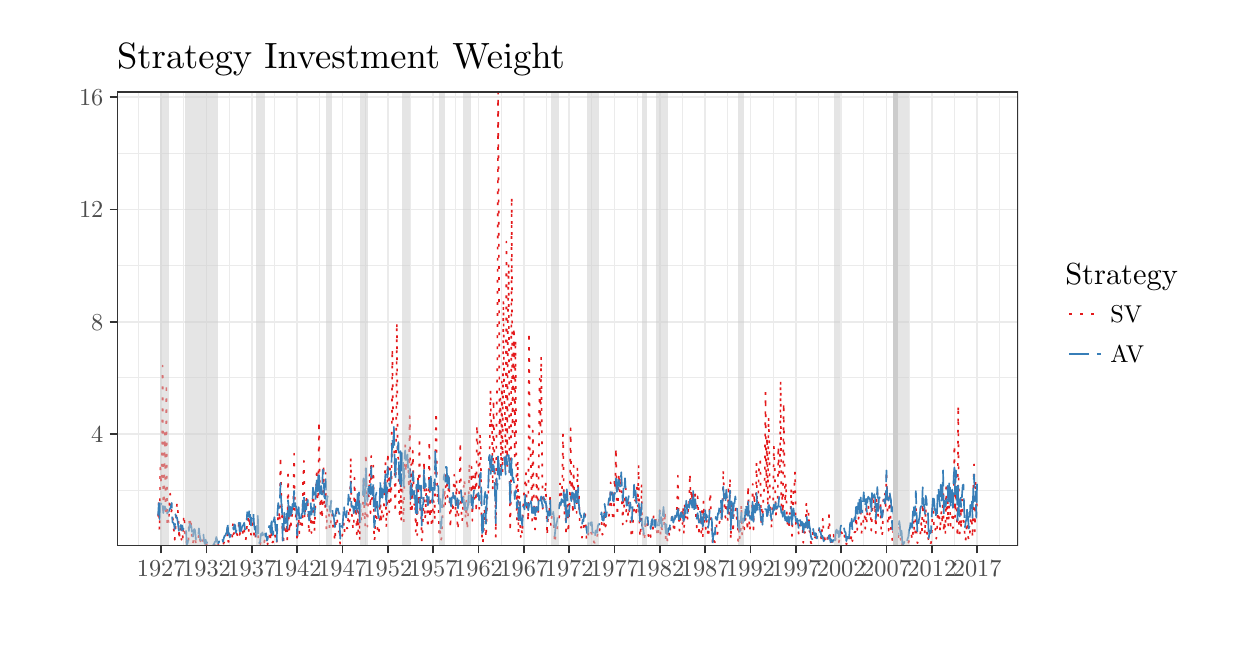
\begin{tikzpicture}[x=1pt,y=1pt]
\definecolor{fillColor}{RGB}{255,255,255}
\path[use as bounding box,fill=fillColor,fill opacity=0.00] (0,0) rectangle (426.79,216.81);
\begin{scope}
\path[clip] (  0.00,  0.00) rectangle (426.79,216.81);
\definecolor{drawColor}{RGB}{255,255,255}
\definecolor{fillColor}{RGB}{255,255,255}

\path[draw=drawColor,line width= 0.6pt,line join=round,line cap=round,fill=fillColor] (  0.00,  0.00) rectangle (426.79,216.81);
\end{scope}
\begin{scope}
\path[clip] ( 32.32, 29.59) rectangle (357.87,193.67);
\definecolor{fillColor}{RGB}{255,255,255}

\path[fill=fillColor] ( 32.32, 29.59) rectangle (357.87,193.67);
\definecolor{drawColor}{gray}{0.92}

\path[draw=drawColor,line width= 0.3pt,line join=round] ( 32.32, 49.71) --
	(357.87, 49.71);

\path[draw=drawColor,line width= 0.3pt,line join=round] ( 32.32, 90.28) --
	(357.87, 90.28);

\path[draw=drawColor,line width= 0.3pt,line join=round] ( 32.32,130.86) --
	(357.87,130.86);

\path[draw=drawColor,line width= 0.3pt,line join=round] ( 32.32,171.43) --
	(357.87,171.43);

\path[draw=drawColor,line width= 0.3pt,line join=round] ( 40.06, 29.59) --
	( 40.06,193.67);

\path[draw=drawColor,line width= 0.3pt,line join=round] ( 56.44, 29.59) --
	( 56.44,193.67);

\path[draw=drawColor,line width= 0.3pt,line join=round] ( 72.82, 29.59) --
	( 72.82,193.67);

\path[draw=drawColor,line width= 0.3pt,line join=round] ( 89.21, 29.59) --
	( 89.21,193.67);

\path[draw=drawColor,line width= 0.3pt,line join=round] (105.58, 29.59) --
	(105.58,193.67);

\path[draw=drawColor,line width= 0.3pt,line join=round] (121.96, 29.59) --
	(121.96,193.67);

\path[draw=drawColor,line width= 0.3pt,line join=round] (138.35, 29.59) --
	(138.35,193.67);

\path[draw=drawColor,line width= 0.3pt,line join=round] (154.73, 29.59) --
	(154.73,193.67);

\path[draw=drawColor,line width= 0.3pt,line join=round] (171.11, 29.59) --
	(171.11,193.67);

\path[draw=drawColor,line width= 0.3pt,line join=round] (187.49, 29.59) --
	(187.49,193.67);

\path[draw=drawColor,line width= 0.3pt,line join=round] (203.87, 29.59) --
	(203.87,193.67);

\path[draw=drawColor,line width= 0.3pt,line join=round] (220.25, 29.59) --
	(220.25,193.67);

\path[draw=drawColor,line width= 0.3pt,line join=round] (236.63, 29.59) --
	(236.63,193.67);

\path[draw=drawColor,line width= 0.3pt,line join=round] (253.01, 29.59) --
	(253.01,193.67);

\path[draw=drawColor,line width= 0.3pt,line join=round] (269.39, 29.59) --
	(269.39,193.67);

\path[draw=drawColor,line width= 0.3pt,line join=round] (285.77, 29.59) --
	(285.77,193.67);

\path[draw=drawColor,line width= 0.3pt,line join=round] (302.15, 29.59) --
	(302.15,193.67);

\path[draw=drawColor,line width= 0.3pt,line join=round] (318.53, 29.59) --
	(318.53,193.67);

\path[draw=drawColor,line width= 0.3pt,line join=round] (334.91, 29.59) --
	(334.91,193.67);

\path[draw=drawColor,line width= 0.3pt,line join=round] (351.30, 29.59) --
	(351.30,193.67);

\path[draw=drawColor,line width= 0.6pt,line join=round] ( 32.32, 69.99) --
	(357.87, 69.99);

\path[draw=drawColor,line width= 0.6pt,line join=round] ( 32.32,110.57) --
	(357.87,110.57);

\path[draw=drawColor,line width= 0.6pt,line join=round] ( 32.32,151.14) --
	(357.87,151.14);

\path[draw=drawColor,line width= 0.6pt,line join=round] ( 32.32,191.72) --
	(357.87,191.72);

\path[draw=drawColor,line width= 0.6pt,line join=round] ( 48.25, 29.59) --
	( 48.25,193.67);

\path[draw=drawColor,line width= 0.6pt,line join=round] ( 64.63, 29.59) --
	( 64.63,193.67);

\path[draw=drawColor,line width= 0.6pt,line join=round] ( 81.02, 29.59) --
	( 81.02,193.67);

\path[draw=drawColor,line width= 0.6pt,line join=round] ( 97.40, 29.59) --
	( 97.40,193.67);

\path[draw=drawColor,line width= 0.6pt,line join=round] (113.77, 29.59) --
	(113.77,193.67);

\path[draw=drawColor,line width= 0.6pt,line join=round] (130.15, 29.59) --
	(130.15,193.67);

\path[draw=drawColor,line width= 0.6pt,line join=round] (146.54, 29.59) --
	(146.54,193.67);

\path[draw=drawColor,line width= 0.6pt,line join=round] (162.92, 29.59) --
	(162.92,193.67);

\path[draw=drawColor,line width= 0.6pt,line join=round] (179.30, 29.59) --
	(179.30,193.67);

\path[draw=drawColor,line width= 0.6pt,line join=round] (195.68, 29.59) --
	(195.68,193.67);

\path[draw=drawColor,line width= 0.6pt,line join=round] (212.06, 29.59) --
	(212.06,193.67);

\path[draw=drawColor,line width= 0.6pt,line join=round] (228.44, 29.59) --
	(228.44,193.67);

\path[draw=drawColor,line width= 0.6pt,line join=round] (244.82, 29.59) --
	(244.82,193.67);

\path[draw=drawColor,line width= 0.6pt,line join=round] (261.20, 29.59) --
	(261.20,193.67);

\path[draw=drawColor,line width= 0.6pt,line join=round] (277.59, 29.59) --
	(277.59,193.67);

\path[draw=drawColor,line width= 0.6pt,line join=round] (293.96, 29.59) --
	(293.96,193.67);

\path[draw=drawColor,line width= 0.6pt,line join=round] (310.34, 29.59) --
	(310.34,193.67);

\path[draw=drawColor,line width= 0.6pt,line join=round] (326.72, 29.59) --
	(326.72,193.67);

\path[draw=drawColor,line width= 0.6pt,line join=round] (343.11, 29.59) --
	(343.11,193.67);
\definecolor{drawColor}{RGB}{228,26,28}

\path[draw=drawColor,line width= 0.6pt,dash pattern=on 1pt off 3pt ,line join=round] ( 47.12, 40.23) --
	( 47.40, 46.35) --
	( 47.67, 35.12) --
	( 47.95, 57.83) --
	( 48.22, 52.69) --
	( 48.49, 52.09) --
	( 48.77, 94.67) --
	( 49.02, 40.74) --
	( 49.30, 45.84) --
	( 49.57, 70.42) --
	( 49.85, 42.05) --
	( 50.12, 88.22) --
	( 50.40, 37.82) --
	( 50.67, 39.86) --
	( 50.94, 37.55) --
	( 51.22, 46.52) --
	( 51.49, 48.46) --
	( 51.77, 41.28) --
	( 52.05, 42.50) --
	( 52.31, 42.67) --
	( 52.58, 37.08) --
	( 52.85, 35.05) --
	( 53.13, 31.76) --
	( 53.40, 35.53) --
	( 53.68, 40.23) --
	( 53.96, 45.08) --
	( 54.23, 42.93) --
	( 54.50, 38.21) --
	( 54.77, 31.74) --
	( 55.05, 36.58) --
	( 55.33, 32.94) --
	( 55.58, 31.76) --
	( 55.86, 34.32) --
	( 56.13, 32.02) --
	( 56.40, 40.73) --
	( 56.67, 39.40) --
	( 56.95, 32.87) --
	( 57.23, 33.11) --
	( 57.50, 29.59) --
	( 57.78, 29.70) --
	( 58.05, 30.51) --
	( 58.32, 39.02) --
	( 58.60, 36.07) --
	( 58.85, 39.72) --
	( 59.13, 35.96) --
	( 59.40, 31.66) --
	( 59.68, 30.25) --
	( 59.95, 31.86) --
	( 60.23, 32.06) --
	( 60.50, 32.98) --
	( 60.77, 30.37) --
	( 61.05, 31.01) --
	( 61.32, 30.79) --
	( 61.60, 31.54) --
	( 61.88, 34.29) --
	( 62.13, 32.48) --
	( 62.41, 31.17) --
	( 62.67, 31.45) --
	( 62.95, 29.98) --
	( 63.22, 31.16) --
	( 63.50, 31.93) --
	( 63.78, 30.06) --
	( 64.05, 29.70) --
	( 64.32, 30.46) --
	( 64.59, 29.98) --
	( 64.87, 30.09) --
	( 65.15, 29.87) --
	( 65.41, 30.43) --
	( 65.69, 30.20) --
	( 65.96, 30.09) --
	( 66.24, 29.84) --
	( 66.50, 30.22) --
	( 66.78, 29.79) --
	( 67.06, 29.69) --
	( 67.33, 29.76) --
	( 67.61, 29.94) --
	( 67.88, 30.72) --
	( 68.15, 31.58) --
	( 68.43, 30.36) --
	( 68.68, 29.71) --
	( 68.96, 29.89) --
	( 69.23, 30.39) --
	( 69.51, 29.94) --
	( 69.78, 29.72) --
	( 70.06, 30.37) --
	( 70.33, 30.24) --
	( 70.60, 29.85) --
	( 70.88, 30.67) --
	( 71.15, 31.26) --
	( 71.43, 31.20) --
	( 71.71, 31.40) --
	( 71.96, 31.24) --
	( 72.24, 34.34) --
	( 72.51, 30.97) --
	( 72.78, 31.14) --
	( 73.05, 30.50) --
	( 73.33, 31.24) --
	( 73.61, 31.94) --
	( 73.88, 32.54) --
	( 74.16, 37.40) --
	( 74.42, 33.82) --
	( 74.70, 34.47) --
	( 74.98, 33.57) --
	( 75.23, 32.81) --
	( 75.51, 34.06) --
	( 75.78, 33.40) --
	( 76.06, 34.06) --
	( 76.33, 39.03) --
	( 76.60, 33.50) --
	( 76.88, 35.02) --
	( 77.15, 33.41) --
	( 77.43, 33.52) --
	( 77.70, 34.21) --
	( 77.98, 36.70) --
	( 78.25, 35.38) --
	( 78.51, 32.01) --
	( 78.79, 31.64) --
	( 79.06, 33.60) --
	( 79.34, 38.68) --
	( 79.61, 39.63) --
	( 79.89, 34.88) --
	( 80.17, 40.16) --
	( 80.43, 36.00) --
	( 80.71, 33.54) --
	( 80.98, 36.66) --
	( 81.26, 37.95) --
	( 81.54, 39.56) --
	( 81.79, 33.77) --
	( 82.07, 31.49) --
	( 82.34, 33.07) --
	( 82.61, 33.60) --
	( 82.88, 35.11) --
	( 83.16, 36.93) --
	( 83.44, 30.14) --
	( 83.71, 29.77) --
	( 83.99, 30.02) --
	( 84.26, 31.27) --
	( 84.53, 30.81) --
	( 84.81, 31.13) --
	( 85.06, 30.44) --
	( 85.34, 30.13) --
	( 85.61, 31.54) --
	( 85.89, 30.74) --
	( 86.16, 31.38) --
	( 86.43, 31.69) --
	( 86.71, 30.12) --
	( 86.98, 33.02) --
	( 87.26, 32.49) --
	( 87.53, 34.95) --
	( 87.81, 31.23) --
	( 88.09, 34.03) --
	( 88.34, 30.89) --
	( 88.61, 30.78) --
	( 88.88, 33.84) --
	( 89.16, 33.74) --
	( 89.43, 33.22) --
	( 89.71, 31.29) --
	( 89.99, 30.24) --
	( 90.26, 36.37) --
	( 90.53, 41.47) --
	( 90.80, 42.03) --
	( 91.08, 38.20) --
	( 91.36, 61.86) --
	( 91.62, 47.39) --
	( 91.90, 41.18) --
	( 92.17, 30.02) --
	( 92.44, 30.74) --
	( 92.71, 41.72) --
	( 92.99, 33.39) --
	( 93.27, 33.56) --
	( 93.54, 39.60) --
	( 93.82, 31.64) --
	( 94.09, 55.39) --
	( 94.36, 38.33) --
	( 94.64, 34.21) --
	( 94.89, 41.08) --
	( 95.17, 37.03) --
	( 95.44, 39.96) --
	( 95.72, 42.14) --
	( 95.99, 41.36) --
	( 96.27, 62.88) --
	( 96.54, 42.73) --
	( 96.81, 39.57) --
	( 97.09, 42.57) --
	( 97.36, 31.10) --
	( 97.64, 35.24) --
	( 97.92, 39.93) --
	( 98.17, 34.13) --
	( 98.45, 34.25) --
	( 98.71, 39.41) --
	( 98.99, 38.75) --
	( 99.26, 36.72) --
	( 99.54, 54.23) --
	( 99.82, 60.29) --
	(100.09, 39.40) --
	(100.36, 43.76) --
	(100.63, 45.76) --
	(100.91, 47.40) --
	(101.19, 45.63) --
	(101.44, 38.05) --
	(101.72, 33.86) --
	(101.99, 39.98) --
	(102.27, 40.71) --
	(102.54, 34.21) --
	(102.81, 36.66) --
	(103.09, 50.06) --
	(103.36, 45.25) --
	(103.64, 34.80) --
	(103.91, 42.70) --
	(104.19, 49.28) --
	(104.46, 57.44) --
	(104.72, 47.13) --
	(105.00, 45.79) --
	(105.27, 74.55) --
	(105.55, 49.70) --
	(105.82, 41.10) --
	(106.10, 51.48) --
	(106.37, 39.29) --
	(106.64, 49.20) --
	(106.92, 59.10) --
	(107.19, 44.28) --
	(107.47, 42.60) --
	(107.75, 55.98) --
	(108.00, 35.28) --
	(108.28, 42.88) --
	(108.54, 43.48) --
	(108.82, 42.70) --
	(109.09, 35.85) --
	(109.37, 35.46) --
	(109.65, 39.49) --
	(109.92, 41.44) --
	(110.20, 38.01) --
	(110.46, 35.64) --
	(110.74, 34.15) --
	(111.02, 31.19) --
	(111.27, 36.48) --
	(111.55, 42.05) --
	(111.82, 38.99) --
	(112.10, 36.48) --
	(112.37, 34.93) --
	(112.64, 34.54) --
	(112.92, 30.07) --
	(113.19, 31.19) --
	(113.47, 32.27) --
	(113.74, 33.69) --
	(114.02, 35.04) --
	(114.29, 38.25) --
	(114.55, 34.07) --
	(114.82, 34.33) --
	(115.09, 34.04) --
	(115.37, 36.16) --
	(115.64, 35.61) --
	(115.92, 42.17) --
	(116.20, 37.93) --
	(116.46, 41.27) --
	(116.74, 61.55) --
	(117.01, 41.45) --
	(117.29, 39.94) --
	(117.57, 35.59) --
	(117.83, 35.79) --
	(118.11, 54.19) --
	(118.38, 40.72) --
	(118.65, 42.41) --
	(118.92, 33.71) --
	(119.20, 42.49) --
	(119.48, 34.22) --
	(119.75, 46.93) --
	(120.03, 31.32) --
	(120.29, 42.84) --
	(120.57, 38.20) --
	(120.85, 39.06) --
	(121.10, 40.66) --
	(121.38, 54.36) --
	(121.65, 42.78) --
	(121.93, 36.48) --
	(122.20, 62.91) --
	(122.47, 42.34) --
	(122.75, 36.49) --
	(123.02, 47.94) --
	(123.30, 47.41) --
	(123.57, 56.02) --
	(123.85, 41.34) --
	(124.12, 62.05) --
	(124.38, 46.47) --
	(124.65, 47.50) --
	(124.92, 58.53) --
	(125.20, 31.33) --
	(125.47, 32.68) --
	(125.75, 45.98) --
	(126.03, 40.75) --
	(126.30, 37.15) --
	(126.57, 33.58) --
	(126.84, 33.69) --
	(127.12, 36.95) --
	(127.40, 49.57) --
	(127.65, 37.65) --
	(127.93, 42.59) --
	(128.20, 39.17) --
	(128.48, 39.56) --
	(128.74, 44.23) --
	(129.02, 54.25) --
	(129.30, 59.78) --
	(129.57, 36.09) --
	(129.85, 41.76) --
	(130.12, 63.28) --
	(130.39, 55.50) --
	(130.67, 41.69) --
	(130.93, 57.56) --
	(131.21, 45.79) --
	(131.48, 52.93) --
	(131.76,100.84) --
	(132.03, 74.98) --
	(132.31, 73.05) --
	(132.58, 56.56) --
	(132.85, 41.58) --
	(133.13, 65.21) --
	(133.40,110.41) --
	(133.68, 61.65) --
	(133.96, 61.31) --
	(134.21, 44.85) --
	(134.48, 39.48) --
	(134.75, 52.51) --
	(135.03, 38.50) --
	(135.30, 51.50) --
	(135.58, 47.29) --
	(135.86, 38.02) --
	(136.13, 53.31) --
	(136.40, 66.16) --
	(136.67, 56.12) --
	(136.95, 58.48) --
	(137.23, 59.63) --
	(137.48, 61.49) --
	(137.76, 50.21) --
	(138.03, 76.47) --
	(138.31, 41.99) --
	(138.57, 59.04) --
	(138.85, 41.28) --
	(139.13, 63.93) --
	(139.40, 53.84) --
	(139.68, 44.30) --
	(139.95, 45.59) --
	(140.23, 34.72) --
	(140.50, 51.84) --
	(140.75, 33.41) --
	(141.03, 55.55) --
	(141.30, 44.09) --
	(141.58, 68.74) --
	(141.85, 41.85) --
	(142.13, 42.28) --
	(142.40, 31.23) --
	(142.67, 34.57) --
	(142.95, 42.73) --
	(143.22, 60.22) --
	(143.50, 38.96) --
	(143.78, 41.00) --
	(144.04, 50.99) --
	(144.32, 42.52) --
	(144.58, 35.86) --
	(144.86, 40.57) --
	(145.13, 67.58) --
	(145.41, 39.56) --
	(145.69, 45.90) --
	(145.96, 36.76) --
	(146.23, 36.27) --
	(146.50, 46.07) --
	(146.78, 45.26) --
	(147.06, 38.81) --
	(147.31, 61.75) --
	(147.59, 77.84) --
	(147.86, 54.92) --
	(148.14, 46.64) --
	(148.41, 47.73) --
	(148.68, 34.36) --
	(148.96, 36.61) --
	(149.23, 31.33) --
	(149.51, 32.21) --
	(149.78, 37.62) --
	(150.06, 43.32) --
	(150.33, 43.79) --
	(150.59, 50.40) --
	(150.86, 43.85) --
	(151.13, 55.18) --
	(151.41, 54.28) --
	(151.68, 47.32) --
	(151.96, 46.77) --
	(152.24, 55.73) --
	(152.50, 42.84) --
	(152.78, 35.84) --
	(153.05, 47.05) --
	(153.33, 46.46) --
	(153.61, 41.72) --
	(153.86, 49.20) --
	(154.14, 55.29) --
	(154.41, 52.79) --
	(154.68, 39.91) --
	(154.95, 53.22) --
	(155.23, 38.55) --
	(155.51, 35.31) --
	(155.78, 45.60) --
	(156.06, 50.92) --
	(156.33, 67.07) --
	(156.60, 44.83) --
	(156.88, 38.25) --
	(157.14, 39.51) --
	(157.42, 45.76) --
	(157.69, 53.74) --
	(157.97, 51.62) --
	(158.24, 39.22) --
	(158.51, 45.92) --
	(158.79, 35.30) --
	(159.06, 38.34) --
	(159.34, 46.62) --
	(159.61, 59.55) --
	(159.89, 48.11) --
	(160.16, 49.51) --
	(160.42, 58.12) --
	(160.69, 38.62) --
	(160.96, 54.74) --
	(161.24, 48.95) --
	(161.51, 46.54) --
	(161.79, 56.89) --
	(162.07, 41.60) --
	(162.34, 73.27) --
	(162.61, 65.85) --
	(162.88, 61.66) --
	(163.16, 42.90) --
	(163.44, 70.10) --
	(163.69, 64.91) --
	(163.97, 40.67) --
	(164.24, 30.33) --
	(164.51, 31.02) --
	(164.78, 35.27) --
	(165.06, 42.75) --
	(165.34, 39.16) --
	(165.61, 32.44) --
	(165.89, 41.85) --
	(166.16, 47.79) --
	(166.43, 46.92) --
	(166.71, 58.93) --
	(166.96, 65.79) --
	(167.24, 85.85) --
	(167.51, 71.92) --
	(167.79, 73.86) --
	(168.06, 49.70) --
	(168.34, 82.36) --
	(168.61, 61.68) --
	(168.88, 54.56) --
	(169.16, 32.53) --
	(169.43, 74.21) --
	(169.71, 96.23) --
	(169.99,193.67) --
	(170.25,141.45) --
	(170.52, 68.56) --
	(170.79, 82.79) --
	(171.07, 55.88) --
	(171.34, 88.94) --
	(171.62, 56.06) --
	(171.90,118.36) --
	(172.17, 83.73) --
	(172.44, 77.35) --
	(172.71, 58.46) --
	(172.99,139.51) --
	(173.27, 57.07) --
	(173.52,111.22) --
	(173.80,131.56) --
	(174.07, 61.86) --
	(174.35, 34.72) --
	(174.61, 49.02) --
	(174.89,155.71) --
	(175.17, 70.66) --
	(175.44, 92.87) --
	(175.72,108.55) --
	(175.99, 61.82) --
	(176.26,104.10) --
	(176.54, 61.04) --
	(176.79, 39.05) --
	(177.07, 60.42) --
	(177.34, 34.31) --
	(177.62, 47.81) --
	(177.89, 39.44) --
	(178.17, 32.72) --
	(178.44, 35.77) --
	(178.71, 33.49) --
	(178.99, 42.25) --
	(179.26, 47.04) --
	(179.54, 51.21) --
	(179.82, 52.80) --
	(180.07, 55.93) --
	(180.35, 42.73) --
	(180.62, 42.26) --
	(180.89, 38.30) --
	(181.16,106.74) --
	(181.44, 63.23) --
	(181.72, 64.05) --
	(181.99, 54.43) --
	(182.27, 38.62) --
	(182.53, 71.25) --
	(182.81, 50.13) --
	(183.09, 40.38) --
	(183.35, 35.45) --
	(183.63, 37.57) --
	(183.90, 57.11) --
	(184.18, 46.31) --
	(184.45, 40.50) --
	(184.72, 62.51) --
	(185.00, 89.98) --
	(185.27, 71.54) --
	(185.55, 98.01) --
	(185.82, 67.23) --
	(186.10, 42.94) --
	(186.37, 46.72) --
	(186.62, 46.60) --
	(186.90, 46.26) --
	(187.17, 52.84) --
	(187.45, 43.23) --
	(187.72, 33.29) --
	(188.00, 39.29) --
	(188.28, 40.23) --
	(188.54, 42.20) --
	(188.82, 48.04) --
	(189.09, 36.62) --
	(189.37, 40.14) --
	(189.65, 39.79) --
	(189.90, 38.68) --
	(190.18, 36.07) --
	(190.45, 30.48) --
	(190.72, 32.86) --
	(190.99, 34.59) --
	(191.27, 34.68) --
	(191.55, 38.03) --
	(191.82, 38.78) --
	(192.10, 40.31) --
	(192.37, 52.11) --
	(192.64, 50.77) --
	(192.92, 47.45) --
	(193.17, 51.84) --
	(193.45, 70.09) --
	(193.72, 49.36) --
	(194.00, 39.46) --
	(194.27, 48.24) --
	(194.54, 33.16) --
	(194.82, 47.67) --
	(195.09, 44.85) --
	(195.37, 34.31) --
	(195.64, 41.00) --
	(195.92, 47.96) --
	(196.20, 72.08) --
	(196.46, 45.83) --
	(196.73, 53.72) --
	(197.00, 41.12) --
	(197.28, 58.56) --
	(197.55, 45.94) --
	(197.83, 47.88) --
	(198.11, 49.58) --
	(198.37, 41.43) --
	(198.65, 58.13) --
	(198.92, 49.71) --
	(199.20, 47.52) --
	(199.48, 37.91) --
	(199.73, 35.85) --
	(200.01, 36.46) --
	(200.28, 32.49) --
	(200.55, 34.23) --
	(200.82, 35.22) --
	(201.10, 38.96) --
	(201.38, 42.61) --
	(201.65, 36.96) --
	(201.93, 32.05) --
	(202.20, 31.35) --
	(202.47, 32.62) --
	(202.75, 35.27) --
	(203.00, 35.90) --
	(203.28, 35.48) --
	(203.55, 34.60) --
	(203.83, 33.77) --
	(204.10, 31.51) --
	(204.38, 31.85) --
	(204.65, 30.86) --
	(204.92, 30.66) --
	(205.20, 32.46) --
	(205.47, 32.16) --
	(205.75, 32.57) --
	(206.03, 34.83) --
	(206.28, 33.85) --
	(206.56, 34.67) --
	(206.82, 35.98) --
	(207.10, 38.05) --
	(207.37, 38.42) --
	(207.65, 33.58) --
	(207.93, 34.04) --
	(208.20, 34.92) --
	(208.47, 42.77) --
	(208.74, 36.50) --
	(209.02, 37.21) --
	(209.30, 37.76) --
	(209.56, 38.66) --
	(209.84, 39.41) --
	(210.11, 40.88) --
	(210.39, 42.27) --
	(210.65, 52.53) --
	(210.93, 44.29) --
	(211.21, 43.25) --
	(211.48, 38.49) --
	(211.76, 39.22) --
	(212.03, 54.00) --
	(212.30, 49.52) --
	(212.58, 64.94) --
	(212.83, 46.87) --
	(213.11, 40.38) --
	(213.38, 48.65) --
	(213.66, 55.89) --
	(213.93, 48.85) --
	(214.21, 52.31) --
	(214.48, 54.65) --
	(214.75, 45.44) --
	(215.03, 37.25) --
	(215.30, 46.65) --
	(215.58, 43.18) --
	(215.86, 48.00) --
	(216.11, 50.35) --
	(216.39, 38.36) --
	(216.65, 41.34) --
	(216.93, 40.70) --
	(217.20, 45.64) --
	(217.48, 40.89) --
	(217.76, 39.59) --
	(218.03, 34.71) --
	(218.31, 32.37) --
	(218.57, 35.36) --
	(218.85, 40.34) --
	(219.13, 42.77) --
	(219.38, 46.02) --
	(219.66, 45.97) --
	(219.93, 40.10) --
	(220.21, 51.14) --
	(220.48, 43.83) --
	(220.75, 58.93) --
	(221.03, 37.64) --
	(221.30, 32.67) --
	(221.58, 36.38) --
	(221.85, 52.15) --
	(222.13, 35.10) --
	(222.40, 35.38) --
	(222.66, 31.40) --
	(222.94, 33.02) --
	(223.21, 37.28) --
	(223.49, 37.79) --
	(223.76, 39.04) --
	(224.04, 35.15) --
	(224.31, 33.05) --
	(224.58, 33.87) --
	(224.86, 34.96) --
	(225.13, 32.73) --
	(225.41, 35.36) --
	(225.69, 35.60) --
	(225.94, 35.73) --
	(226.22, 41.21) --
	(226.49, 40.90) --
	(226.76, 39.43) --
	(227.03, 39.11) --
	(227.31, 35.26) --
	(227.59, 32.72) --
	(227.86, 34.65) --
	(228.14, 37.16) --
	(228.40, 42.45) --
	(228.68, 33.46) --
	(228.96, 36.33) --
	(229.21, 35.48) --
	(229.49, 39.76) --
	(229.76, 42.29) --
	(230.04, 36.61) --
	(230.31, 42.10) --
	(230.58, 31.50) --
	(230.86, 35.05) --
	(231.13, 31.51) --
	(231.41, 31.59) --
	(231.68, 34.41) --
	(231.96, 32.75) --
	(232.23, 35.98) --
	(232.49, 38.12) --
	(232.76, 40.01) --
	(233.03, 38.51) --
	(233.31, 37.08) --
	(233.58, 34.33) --
	(233.86, 38.12) --
	(234.14, 40.46) --
	(234.41, 39.93) --
	(234.68, 44.49) --
	(234.95, 54.95) --
	(235.23, 42.60) --
	(235.51, 35.03) --
	(235.77, 38.51) --
	(236.05, 41.85) --
	(236.32, 42.32) --
	(236.59, 37.45) --
	(236.86, 43.99) --
	(237.14, 33.62) --
	(237.42, 44.20) --
	(237.69, 39.81) --
	(237.97, 41.69) --
	(238.24, 40.71) --
	(238.51, 38.96) --
	(238.79, 45.34) --
	(239.04, 44.82) --
	(239.32, 55.76) --
	(239.59, 45.40) --
	(239.87, 49.97) --
	(240.14, 45.33) --
	(240.42, 49.57) --
	(240.69, 43.93) --
	(240.96, 45.24) --
	(241.24, 48.19) --
	(241.51, 40.29) --
	(241.79, 36.20) --
	(242.07, 47.46) --
	(242.32, 42.31) --
	(242.59, 34.68) --
	(242.86, 40.43) --
	(243.14, 38.93) --
	(243.41, 34.25) --
	(243.69, 42.75) --
	(243.97, 32.47) --
	(244.24, 45.88) --
	(244.51, 37.33) --
	(244.78, 40.05) --
	(245.06, 35.64) --
	(245.34, 38.93) --
	(245.59, 36.15) --
	(245.87, 32.49) --
	(246.14, 34.88) --
	(246.42, 45.78) --
	(246.68, 48.88) --
	(246.96, 36.93) --
	(247.24, 34.96) --
	(247.51, 29.60) --
	(247.79, 31.26) --
	(248.06, 31.38) --
	(248.34, 30.87) --
	(248.61, 37.38) --
	(248.87, 37.57) --
	(249.15, 33.43) --
	(249.42, 35.04) --
	(249.70, 36.07) --
	(249.97, 37.98) --
	(250.25, 39.12) --
	(250.52, 42.76) --
	(250.79, 38.94) --
	(251.07, 39.14) --
	(251.34, 57.10) --
	(251.62, 48.29) --
	(251.90, 41.57) --
	(252.15, 39.71) --
	(252.43, 49.26) --
	(252.69, 44.27) --
	(252.97, 38.44) --
	(253.24, 51.55) --
	(253.52, 40.38) --
	(253.80, 54.19) --
	(254.07, 31.75) --
	(254.34, 45.31) --
	(254.61, 42.44) --
	(254.89, 34.30) --
	(255.17, 42.41) --
	(255.42, 42.92) --
	(255.70, 42.07) --
	(255.97, 43.11) --
	(256.25, 39.31) --
	(256.52, 38.82) --
	(256.79, 31.29) --
	(257.07, 35.75) --
	(257.34, 32.04) --
	(257.62, 34.84) --
	(257.89, 44.70) --
	(258.17, 33.11) --
	(258.44, 34.80) --
	(258.70, 38.01) --
	(258.97, 35.50) --
	(259.24, 37.32) --
	(259.52, 41.56) --
	(259.79, 42.15) --
	(260.07, 34.99) --
	(260.35, 51.29) --
	(260.61, 39.54) --
	(260.89, 34.93) --
	(261.16, 36.99) --
	(261.44, 41.21) --
	(261.72, 41.47) --
	(261.98, 51.93) --
	(262.26, 35.48) --
	(262.53, 48.45) --
	(262.80, 43.24) --
	(263.07, 43.26) --
	(263.35, 59.65) --
	(263.63, 42.23) --
	(263.90, 42.09) --
	(264.18, 56.06) --
	(264.44, 60.09) --
	(264.72, 60.35) --
	(265.00, 37.12) --
	(265.25, 42.99) --
	(265.53, 40.63) --
	(265.80, 45.69) --
	(266.08, 49.51) --
	(266.35, 54.70) --
	(266.62, 85.12) --
	(266.90, 49.99) --
	(267.17, 68.95) --
	(267.45, 43.77) --
	(267.72, 76.12) --
	(268.00, 65.10) --
	(268.27, 39.99) --
	(268.53, 40.75) --
	(268.80, 35.86) --
	(269.07, 43.60) --
	(269.35, 43.46) --
	(269.62, 65.79) --
	(269.90, 58.63) --
	(270.18, 45.81) --
	(270.45, 40.15) --
	(270.72, 44.06) --
	(270.99, 44.70) --
	(271.27, 65.65) --
	(271.55, 55.28) --
	(271.80, 56.14) --
	(272.08, 89.34) --
	(272.35, 43.99) --
	(272.62, 47.20) --
	(272.89, 41.32) --
	(273.17, 81.28) --
	(273.45, 59.46) --
	(273.72, 45.08) --
	(274.00, 52.44) --
	(274.27, 41.42) --
	(274.54, 37.52) --
	(274.82, 40.49) --
	(275.08, 36.37) --
	(275.36, 41.43) --
	(275.63, 40.48) --
	(275.91, 50.37) --
	(276.18, 33.10) --
	(276.45, 39.72) --
	(276.73, 50.85) --
	(277.00, 50.38) --
	(277.28, 56.45) --
	(277.55, 37.44) --
	(277.83, 39.99) --
	(278.11, 37.86) --
	(278.36, 35.79) --
	(278.63, 33.67) --
	(278.90, 36.14) --
	(279.18, 37.41) --
	(279.45, 37.08) --
	(279.73, 35.36) --
	(280.01, 35.75) --
	(280.28, 30.66) --
	(280.55, 33.66) --
	(280.82, 34.61) --
	(281.10, 33.64) --
	(281.38, 45.32) --
	(281.63, 41.03) --
	(281.91, 35.56) --
	(282.18, 41.80) --
	(282.46, 34.87) --
	(282.72, 34.60) --
	(283.00, 30.62) --
	(283.28, 30.53) --
	(283.55, 31.08) --
	(283.83, 35.15) --
	(284.10, 33.13) --
	(284.38, 32.82) --
	(284.65, 32.46) --
	(284.90, 32.94) --
	(285.18, 33.34) --
	(285.45, 32.99) --
	(285.73, 33.79) --
	(286.00, 35.63) --
	(286.28, 33.15) --
	(286.55, 33.41) --
	(286.82, 31.78) --
	(287.10, 36.66) --
	(287.37, 39.69) --
	(287.65, 31.12) --
	(287.93, 32.97) --
	(288.19, 30.97) --
	(288.47, 30.26) --
	(288.73, 30.84) --
	(289.01, 32.55) --
	(289.28, 32.97) --
	(289.56, 40.70) --
	(289.84, 34.62) --
	(290.11, 30.75) --
	(290.38, 31.74) --
	(290.65, 30.73) --
	(290.93, 30.96) --
	(291.21, 33.59) --
	(291.46, 30.78) --
	(291.74, 30.62) --
	(292.01, 32.89) --
	(292.29, 35.39) --
	(292.56, 32.95) --
	(292.83, 34.67) --
	(293.11, 30.81) --
	(293.38, 32.25) --
	(293.66, 34.66) --
	(293.93, 34.49) --
	(294.21, 34.23) --
	(294.48, 33.31) --
	(294.73, 34.58) --
	(295.01, 34.17) --
	(295.28, 32.08) --
	(295.56, 32.58) --
	(295.83, 30.13) --
	(296.11, 30.57) --
	(296.39, 31.00) --
	(296.65, 30.33) --
	(296.93, 31.74) --
	(297.20, 33.57) --
	(297.48, 31.56) --
	(297.76, 33.85) --
	(298.01, 31.25) --
	(298.29, 33.43) --
	(298.56, 34.67) --
	(298.83, 34.40) --
	(299.10, 34.58) --
	(299.38, 40.09) --
	(299.66, 34.71) --
	(299.93, 37.12) --
	(300.21, 39.51) --
	(300.48, 40.78) --
	(300.75, 41.30) --
	(301.03, 42.44) --
	(301.29, 33.98) --
	(301.57, 36.58) --
	(301.84, 37.11) --
	(302.12, 40.84) --
	(302.39, 41.17) --
	(302.66, 35.72) --
	(302.94, 43.03) --
	(303.21, 37.91) --
	(303.49, 43.48) --
	(303.76, 44.30) --
	(304.04, 40.29) --
	(304.31, 41.26) --
	(304.57, 42.20) --
	(304.84, 35.05) --
	(305.11, 40.71) --
	(305.39, 48.16) --
	(305.66, 45.77) --
	(305.94, 42.57) --
	(306.22, 44.92) --
	(306.48, 34.14) --
	(306.76, 46.92) --
	(307.03, 49.25) --
	(307.31, 39.93) --
	(307.59, 44.54) --
	(307.84, 45.38) --
	(308.12, 45.55) --
	(308.39, 35.84) --
	(308.66, 33.06) --
	(308.93, 34.76) --
	(309.21, 47.00) --
	(309.49, 46.26) --
	(309.76, 48.43) --
	(310.04, 43.93) --
	(310.31, 55.01) --
	(310.58, 47.97) --
	(310.86, 35.92) --
	(311.11, 35.04) --
	(311.39, 47.68) --
	(311.66, 42.46) --
	(311.94, 35.99) --
	(312.21, 33.63) --
	(312.49, 31.35) --
	(312.76, 34.79) --
	(313.03, 34.73) --
	(313.31, 31.18) --
	(313.58, 33.29) --
	(313.86, 31.63) --
	(314.14, 32.37) --
	(314.40, 30.91) --
	(314.67, 33.13) --
	(314.94, 36.45) --
	(315.22, 33.05) --
	(315.49, 31.71) --
	(315.77, 32.70) --
	(316.05, 29.85) --
	(316.32, 29.59) --
	(316.59, 29.67) --
	(316.86, 29.88) --
	(317.14, 30.17) --
	(317.42, 30.47) --
	(317.67, 29.88) --
	(317.95, 30.60) --
	(318.22, 30.77) --
	(318.50, 31.76) --
	(318.76, 31.95) --
	(319.04, 33.21) --
	(319.32, 33.90) --
	(319.59, 31.56) --
	(319.87, 33.95) --
	(320.14, 38.99) --
	(320.41, 34.29) --
	(320.69, 33.27) --
	(320.94, 44.58) --
	(321.22, 34.36) --
	(321.49, 30.54) --
	(321.77, 31.04) --
	(322.04, 32.29) --
	(322.32, 32.81) --
	(322.59, 34.19) --
	(322.86, 37.83) --
	(323.14, 34.42) --
	(323.41, 45.04) --
	(323.69, 39.35) --
	(323.97, 37.74) --
	(324.22, 33.63) --
	(324.50, 43.36) --
	(324.76, 37.57) --
	(325.04, 33.32) --
	(325.31, 34.32) --
	(325.59, 29.89) --
	(325.87, 30.80) --
	(326.14, 30.63) --
	(326.42, 30.59) --
	(326.68, 32.50) --
	(326.96, 44.17) --
	(327.24, 43.57) --
	(327.50, 36.54) --
	(327.78, 34.69) --
	(328.05, 35.79) --
	(328.33, 32.11) --
	(328.59, 35.42) --
	(328.87, 42.13) --
	(329.15, 38.68) --
	(329.42, 40.53) --
	(329.70, 34.64) --
	(329.97, 40.47) --
	(330.25, 42.25) --
	(330.52, 37.40) --
	(330.77, 53.89) --
	(331.05, 34.51) --
	(331.32, 38.86) --
	(331.60, 33.59) --
	(331.87, 50.78) --
	(332.15, 39.26) --
	(332.42, 46.32) --
	(332.69, 36.41) --
	(332.97, 44.40) --
	(333.24, 43.65) --
	(333.52, 36.83) --
	(333.80, 37.59) --
	(334.05, 40.18) --
	(334.33, 35.93) --
	(334.60, 46.93) --
	(334.87, 66.06) --
	(335.14, 39.75) --
	(335.42, 50.86) --
	(335.70, 42.65) --
	(335.97, 32.76) --
	(336.25, 80.37) --
	(336.52, 34.17) --
	(336.79, 34.04) --
	(337.07, 43.59) --
	(337.32, 35.65) --
	(337.60, 46.33) --
	(337.87, 41.82) --
	(338.15, 38.67) --
	(338.42, 37.91) --
	(338.69, 31.30) --
	(338.97, 31.90) --
	(339.24, 35.99) --
	(339.52, 38.28) --
	(339.79, 33.05) --
	(340.07, 31.59) --
	(340.35, 32.68) --
	(340.61, 36.66) --
	(340.88, 40.18) --
	(341.15, 38.83) --
	(341.43, 32.42) --
	(341.70, 49.51) --
	(341.98, 59.00) --
	(342.26, 34.77) --
	(342.52, 53.33) --
	(342.80, 40.24) --
	(343.07, 46.96);
\definecolor{drawColor}{RGB}{55,126,184}

\path[draw=drawColor,line width= 0.6pt,dash pattern=on 7pt off 3pt ,line join=round] ( 47.12, 40.53) --
	( 47.40, 45.03) --
	( 47.67, 39.24) --
	( 47.95, 44.93) --
	( 48.22, 44.57) --
	( 48.49, 46.12) --
	( 48.77, 45.20) --
	( 49.02, 41.41) --
	( 49.30, 43.64) --
	( 49.57, 43.82) --
	( 49.85, 42.74) --
	( 50.12, 43.96) --
	( 50.40, 41.20) --
	( 50.67, 41.86) --
	( 50.94, 41.82) --
	( 51.22, 42.84) --
	( 51.49, 42.91) --
	( 51.77, 44.01) --
	( 52.05, 45.08) --
	( 52.31, 38.11) --
	( 52.58, 37.99) --
	( 52.85, 37.55) --
	( 53.13, 35.55) --
	( 53.40, 40.98) --
	( 53.68, 39.69) --
	( 53.96, 39.83) --
	( 54.23, 38.29) --
	( 54.50, 35.99) --
	( 54.77, 34.06) --
	( 55.05, 35.82) --
	( 55.33, 37.13) --
	( 55.58, 35.14) --
	( 55.86, 36.90) --
	( 56.13, 35.34) --
	( 56.40, 36.46) --
	( 56.67, 36.54) --
	( 56.95, 34.91) --
	( 57.23, 35.33) --
	( 57.50, 30.02) --
	( 57.78, 30.43) --
	( 58.05, 32.07) --
	( 58.32, 35.91) --
	( 58.60, 37.53) --
	( 58.85, 36.31) --
	( 59.13, 36.82) --
	( 59.40, 33.98) --
	( 59.68, 32.12) --
	( 59.95, 35.03) --
	( 60.23, 35.63) --
	( 60.50, 35.09) --
	( 60.77, 31.90) --
	( 61.05, 32.83) --
	( 61.32, 32.21) --
	( 61.60, 32.62) --
	( 61.88, 35.87) --
	( 62.13, 33.53) --
	( 62.41, 31.94) --
	( 62.67, 31.66) --
	( 62.95, 31.01) --
	( 63.22, 33.45) --
	( 63.50, 33.65) --
	( 63.78, 31.03) --
	( 64.05, 30.26) --
	( 64.32, 31.81) --
	( 64.59, 30.52) --
	( 64.87, 30.83) --
	( 65.15, 30.78) --
	( 65.41, 31.04) --
	( 65.69, 30.72) --
	( 65.96, 30.65) --
	( 66.24, 30.23) --
	( 66.50, 29.76) --
	( 66.78, 30.24) --
	( 67.06, 29.93) --
	( 67.33, 30.17) --
	( 67.61, 31.02) --
	( 67.88, 31.00) --
	( 68.15, 32.75) --
	( 68.43, 31.79) --
	( 68.68, 30.40) --
	( 68.96, 30.64) --
	( 69.23, 31.17) --
	( 69.51, 30.95) --
	( 69.78, 30.51) --
	( 70.06, 32.31) --
	( 70.33, 32.04) --
	( 70.60, 30.97) --
	( 70.88, 32.43) --
	( 71.15, 33.24) --
	( 71.43, 33.22) --
	( 71.71, 34.06) --
	( 71.96, 34.50) --
	( 72.24, 38.28) --
	( 72.51, 33.55) --
	( 72.78, 34.14) --
	( 73.05, 32.62) --
	( 73.33, 33.56) --
	( 73.61, 34.56) --
	( 73.88, 34.52) --
	( 74.16, 36.35) --
	( 74.42, 35.42) --
	( 74.70, 37.32) --
	( 74.98, 36.93) --
	( 75.23, 34.30) --
	( 75.51, 35.52) --
	( 75.78, 35.14) --
	( 76.06, 36.50) --
	( 76.33, 37.93) --
	( 76.60, 34.75) --
	( 76.88, 38.30) --
	( 77.15, 34.88) --
	( 77.43, 36.32) --
	( 77.70, 36.97) --
	( 77.98, 36.98) --
	( 78.25, 37.92) --
	( 78.51, 35.54) --
	( 78.79, 35.58) --
	( 79.06, 37.69) --
	( 79.34, 41.75) --
	( 79.61, 40.65) --
	( 79.89, 40.05) --
	( 80.17, 43.17) --
	( 80.43, 39.95) --
	( 80.71, 36.90) --
	( 80.98, 39.71) --
	( 81.26, 39.63) --
	( 81.54, 41.67) --
	( 81.79, 37.32) --
	( 82.07, 35.40) --
	( 82.34, 37.74) --
	( 82.61, 32.89) --
	( 82.88, 36.61) --
	( 83.16, 40.43) --
	( 83.44, 31.89) --
	( 83.71, 30.54) --
	( 83.99, 31.02) --
	( 84.26, 33.89) --
	( 84.53, 33.26) --
	( 84.81, 34.45) --
	( 85.06, 32.64) --
	( 85.34, 31.84) --
	( 85.61, 33.95) --
	( 85.89, 33.06) --
	( 86.16, 34.16) --
	( 86.43, 31.45) --
	( 86.71, 31.85) --
	( 86.98, 35.21) --
	( 87.26, 36.77) --
	( 87.53, 36.38) --
	( 87.81, 34.31) --
	( 88.09, 39.86) --
	( 88.34, 34.62) --
	( 88.61, 33.41) --
	( 88.88, 38.37) --
	( 89.16, 39.92) --
	( 89.43, 37.67) --
	( 89.71, 34.93) --
	( 89.99, 31.13) --
	( 90.26, 41.39) --
	( 90.53, 45.03) --
	( 90.80, 43.22) --
	( 91.08, 44.43) --
	( 91.36, 52.25) --
	( 91.62, 45.66) --
	( 91.90, 42.65) --
	( 92.17, 31.42) --
	( 92.44, 32.97) --
	( 92.71, 41.56) --
	( 92.99, 37.79) --
	( 93.27, 37.93) --
	( 93.54, 41.18) --
	( 93.82, 35.27) --
	( 94.09, 46.03) --
	( 94.36, 42.40) --
	( 94.64, 40.10) --
	( 94.89, 43.67) --
	( 95.17, 40.81) --
	( 95.44, 41.83) --
	( 95.72, 44.70) --
	( 95.99, 42.61) --
	( 96.27, 49.43) --
	( 96.54, 46.03) --
	( 96.81, 43.62) --
	( 97.09, 43.79) --
	( 97.36, 33.38) --
	( 97.64, 37.53) --
	( 97.92, 43.55) --
	( 98.17, 38.13) --
	( 98.45, 37.80) --
	( 98.71, 39.46) --
	( 98.99, 40.95) --
	( 99.26, 41.31) --
	( 99.54, 47.67) --
	( 99.82, 48.16) --
	(100.09, 40.96) --
	(100.36, 44.86) --
	(100.63, 42.69) --
	(100.91, 45.39) --
	(101.19, 46.19) --
	(101.44, 41.40) --
	(101.72, 38.68) --
	(101.99, 41.10) --
	(102.27, 45.20) --
	(102.54, 40.83) --
	(102.81, 42.87) --
	(103.09, 50.61) --
	(103.36, 49.24) --
	(103.64, 40.54) --
	(103.91, 44.02) --
	(104.19, 50.66) --
	(104.46, 53.23) --
	(104.72, 49.31) --
	(105.00, 54.48) --
	(105.27, 56.73) --
	(105.55, 46.72) --
	(105.82, 47.02) --
	(106.10, 51.22) --
	(106.37, 48.06) --
	(106.64, 57.10) --
	(106.92, 56.56) --
	(107.19, 47.27) --
	(107.47, 46.62) --
	(107.75, 53.70) --
	(108.00, 43.84) --
	(108.28, 47.56) --
	(108.54, 47.06) --
	(108.82, 45.07) --
	(109.09, 43.41) --
	(109.37, 41.82) --
	(109.65, 45.93) --
	(109.92, 44.41) --
	(110.20, 41.39) --
	(110.46, 40.56) --
	(110.74, 39.00) --
	(111.02, 36.31) --
	(111.27, 41.31) --
	(111.55, 43.10) --
	(111.82, 42.43) --
	(112.10, 43.09) --
	(112.37, 41.45) --
	(112.64, 41.41) --
	(112.92, 32.11) --
	(113.19, 34.74) --
	(113.47, 36.78) --
	(113.74, 36.11) --
	(114.02, 40.14) --
	(114.29, 44.33) --
	(114.55, 40.80) --
	(114.82, 40.93) --
	(115.09, 39.78) --
	(115.37, 42.43) --
	(115.64, 41.85) --
	(115.92, 48.09) --
	(116.20, 45.81) --
	(116.46, 46.29) --
	(116.74, 52.61) --
	(117.01, 43.62) --
	(117.29, 43.95) --
	(117.57, 43.92) --
	(117.83, 41.37) --
	(118.11, 44.99) --
	(118.38, 43.05) --
	(118.65, 45.30) --
	(118.92, 41.30) --
	(119.20, 48.33) --
	(119.48, 42.67) --
	(119.75, 48.93) --
	(120.03, 36.55) --
	(120.29, 45.21) --
	(120.57, 46.25) --
	(120.85, 46.79) --
	(121.10, 47.07) --
	(121.38, 53.95) --
	(121.65, 52.12) --
	(121.93, 44.36) --
	(122.20, 58.19) --
	(122.47, 50.35) --
	(122.75, 45.68) --
	(123.02, 52.30) --
	(123.30, 51.22) --
	(123.57, 49.16) --
	(123.85, 48.17) --
	(124.12, 58.08) --
	(124.38, 50.34) --
	(124.65, 47.90) --
	(124.92, 52.66) --
	(125.20, 36.25) --
	(125.47, 37.95) --
	(125.75, 47.66) --
	(126.03, 48.81) --
	(126.30, 44.65) --
	(126.57, 41.18) --
	(126.84, 39.64) --
	(127.12, 42.78) --
	(127.40, 52.99) --
	(127.65, 47.06) --
	(127.93, 51.11) --
	(128.20, 46.92) --
	(128.48, 50.51) --
	(128.74, 48.22) --
	(129.02, 52.11) --
	(129.30, 55.62) --
	(129.57, 43.33) --
	(129.85, 50.31) --
	(130.12, 58.14) --
	(130.39, 52.88) --
	(130.67, 52.05) --
	(130.93, 51.01) --
	(131.21, 53.72) --
	(131.48, 59.97) --
	(131.76, 68.70) --
	(132.03, 65.06) --
	(132.31, 72.56) --
	(132.58, 61.84) --
	(132.85, 53.49) --
	(133.13, 60.62) --
	(133.40, 61.77) --
	(133.68, 64.54) --
	(133.96, 67.05) --
	(134.21, 55.04) --
	(134.48, 50.89) --
	(134.75, 63.78) --
	(135.03, 51.12) --
	(135.30, 63.12) --
	(135.58, 62.00) --
	(135.86, 50.34) --
	(136.13, 59.94) --
	(136.40, 64.08) --
	(136.67, 58.95) --
	(136.95, 60.36) --
	(137.23, 62.56) --
	(137.48, 56.82) --
	(137.76, 54.28) --
	(138.03, 57.51) --
	(138.31, 46.35) --
	(138.57, 52.19) --
	(138.85, 47.92) --
	(139.13, 56.34) --
	(139.40, 54.28) --
	(139.68, 46.67) --
	(139.95, 47.76) --
	(140.23, 41.41) --
	(140.50, 51.65) --
	(140.75, 41.19) --
	(141.03, 53.14) --
	(141.30, 51.03) --
	(141.58, 51.24) --
	(141.85, 43.08) --
	(142.13, 51.41) --
	(142.40, 36.92) --
	(142.67, 44.32) --
	(142.95, 44.62) --
	(143.22, 57.37) --
	(143.50, 50.46) --
	(143.78, 52.11) --
	(144.04, 49.44) --
	(144.32, 47.08) --
	(144.58, 44.20) --
	(144.86, 44.86) --
	(145.13, 53.36) --
	(145.41, 49.62) --
	(145.69, 54.64) --
	(145.96, 46.70) --
	(146.23, 45.07) --
	(146.50, 51.36) --
	(146.78, 53.16) --
	(147.06, 49.72) --
	(147.31, 64.05) --
	(147.59, 55.93) --
	(147.86, 51.39) --
	(148.14, 51.36) --
	(148.41, 50.92) --
	(148.68, 43.13) --
	(148.96, 46.60) --
	(149.23, 35.91) --
	(149.51, 37.56) --
	(149.78, 45.56) --
	(150.06, 46.98) --
	(150.33, 54.33) --
	(150.59, 55.49) --
	(150.86, 52.69) --
	(151.13, 58.09) --
	(151.41, 58.01) --
	(151.68, 50.70) --
	(151.96, 54.81) --
	(152.24, 53.87) --
	(152.50, 46.49) --
	(152.78, 45.18) --
	(153.05, 43.77) --
	(153.33, 48.43) --
	(153.61, 49.63) --
	(153.86, 47.03) --
	(154.14, 46.73) --
	(154.41, 47.60) --
	(154.68, 44.21) --
	(154.95, 46.12) --
	(155.23, 47.25) --
	(155.51, 43.12) --
	(155.78, 46.24) --
	(156.06, 47.20) --
	(156.33, 48.60) --
	(156.60, 49.66) --
	(156.88, 45.62) --
	(157.14, 45.21) --
	(157.42, 48.35) --
	(157.69, 44.34) --
	(157.97, 42.49) --
	(158.24, 45.17) --
	(158.51, 46.02) --
	(158.79, 42.54) --
	(159.06, 43.60) --
	(159.34, 47.94) --
	(159.61, 45.68) --
	(159.89, 44.82) --
	(160.16, 48.00) --
	(160.42, 44.87) --
	(160.69, 41.94) --
	(160.96, 45.99) --
	(161.24, 49.45) --
	(161.51, 49.97) --
	(161.79, 48.22) --
	(162.07, 48.27) --
	(162.34, 48.71) --
	(162.61, 47.52) --
	(162.88, 48.72) --
	(163.16, 45.98) --
	(163.44, 55.19) --
	(163.69, 55.97) --
	(163.97, 47.43) --
	(164.24, 32.67) --
	(164.51, 34.72) --
	(164.78, 41.30) --
	(165.06, 47.28) --
	(165.34, 49.08) --
	(165.61, 37.50) --
	(165.89, 45.52) --
	(166.16, 50.98) --
	(166.43, 50.57) --
	(166.71, 61.62) --
	(166.96, 62.44) --
	(167.24, 54.99) --
	(167.51, 57.60) --
	(167.79, 62.07) --
	(168.06, 56.90) --
	(168.34, 58.76) --
	(168.61, 56.29) --
	(168.88, 48.25) --
	(169.16, 37.74) --
	(169.43, 53.96) --
	(169.71, 50.10) --
	(169.99, 62.82) --
	(170.25, 58.61) --
	(170.52, 52.85) --
	(170.79, 56.75) --
	(171.07, 55.14) --
	(171.34, 59.54) --
	(171.62, 59.44) --
	(171.90, 60.32) --
	(172.17, 61.58) --
	(172.44, 59.79) --
	(172.71, 55.28) --
	(172.99, 62.31) --
	(173.27, 58.91) --
	(173.52, 61.25) --
	(173.80, 62.39) --
	(174.07, 59.87) --
	(174.35, 43.88) --
	(174.61, 55.18) --
	(174.89, 61.18) --
	(175.17, 53.39) --
	(175.44, 54.23) --
	(175.72, 52.44) --
	(175.99, 46.50) --
	(176.26, 49.62) --
	(176.54, 49.32) --
	(176.79, 43.19) --
	(177.07, 46.05) --
	(177.34, 39.04) --
	(177.62, 45.12) --
	(177.89, 46.16) --
	(178.17, 37.21) --
	(178.44, 39.49) --
	(178.71, 36.89) --
	(178.99, 43.59) --
	(179.26, 43.76) --
	(179.54, 42.74) --
	(179.82, 48.01) --
	(180.07, 44.20) --
	(180.35, 45.11) --
	(180.62, 44.23) --
	(180.89, 42.40) --
	(181.16, 44.09) --
	(181.44, 47.02) --
	(181.72, 46.11) --
	(181.99, 44.61) --
	(182.27, 41.36) --
	(182.53, 44.89) --
	(182.81, 41.43) --
	(183.09, 43.60) --
	(183.35, 41.20) --
	(183.63, 39.50) --
	(183.90, 43.61) --
	(184.18, 42.57) --
	(184.45, 42.42) --
	(184.72, 47.59) --
	(185.00, 46.40) --
	(185.27, 45.91) --
	(185.55, 47.42) --
	(185.82, 45.12) --
	(186.10, 43.48) --
	(186.37, 47.51) --
	(186.62, 45.88) --
	(186.90, 45.11) --
	(187.17, 45.62) --
	(187.45, 43.72) --
	(187.72, 38.37) --
	(188.00, 41.95) --
	(188.28, 42.08) --
	(188.54, 40.42) --
	(188.82, 46.03) --
	(189.09, 40.34) --
	(189.37, 39.87) --
	(189.65, 39.15) --
	(189.90, 41.91) --
	(190.18, 39.70) --
	(190.45, 33.08) --
	(190.72, 36.14) --
	(190.99, 37.11) --
	(191.27, 38.38) --
	(191.55, 40.13) --
	(191.82, 41.70) --
	(192.10, 44.35) --
	(192.37, 45.22) --
	(192.64, 44.27) --
	(192.92, 46.44) --
	(193.17, 46.03) --
	(193.45, 44.93) --
	(193.72, 48.92) --
	(194.00, 43.93) --
	(194.27, 48.18) --
	(194.54, 38.01) --
	(194.82, 50.01) --
	(195.09, 45.87) --
	(195.37, 40.01) --
	(195.64, 41.60) --
	(195.92, 45.85) --
	(196.20, 47.30) --
	(196.46, 45.75) --
	(196.73, 48.93) --
	(197.00, 45.58) --
	(197.28, 48.63) --
	(197.55, 45.15) --
	(197.83, 42.51) --
	(198.11, 49.42) --
	(198.37, 44.37) --
	(198.65, 44.87) --
	(198.92, 50.70) --
	(199.20, 44.28) --
	(199.48, 41.58) --
	(199.73, 40.72) --
	(200.01, 40.43) --
	(200.28, 36.99) --
	(200.55, 39.06) --
	(200.82, 38.41) --
	(201.10, 41.36) --
	(201.38, 40.01) --
	(201.65, 38.40) --
	(201.93, 35.43) --
	(202.20, 33.95) --
	(202.47, 34.73) --
	(202.75, 38.98) --
	(203.00, 39.47) --
	(203.28, 39.46) --
	(203.55, 36.91) --
	(203.83, 38.14) --
	(204.10, 34.38) --
	(204.38, 34.40) --
	(204.65, 33.19) --
	(204.92, 32.19) --
	(205.20, 35.02) --
	(205.47, 35.15) --
	(205.75, 34.27) --
	(206.03, 36.70) --
	(206.28, 37.40) --
	(206.56, 37.26) --
	(206.82, 38.40) --
	(207.10, 40.45) --
	(207.37, 41.68) --
	(207.65, 38.93) --
	(207.93, 38.69) --
	(208.20, 38.86) --
	(208.47, 44.75) --
	(208.74, 42.80) --
	(209.02, 40.05) --
	(209.30, 41.95) --
	(209.56, 41.60) --
	(209.84, 45.13) --
	(210.11, 46.82) --
	(210.39, 45.91) --
	(210.65, 50.44) --
	(210.93, 49.31) --
	(211.21, 49.48) --
	(211.48, 46.03) --
	(211.76, 45.60) --
	(212.03, 48.14) --
	(212.30, 48.81) --
	(212.58, 53.88) --
	(212.83, 49.95) --
	(213.11, 47.75) --
	(213.38, 53.51) --
	(213.66, 53.15) --
	(213.93, 51.20) --
	(214.21, 51.03) --
	(214.48, 56.20) --
	(214.75, 50.01) --
	(215.03, 45.80) --
	(215.30, 50.66) --
	(215.58, 49.26) --
	(215.86, 54.01) --
	(216.11, 48.84) --
	(216.39, 44.11) --
	(216.65, 44.24) --
	(216.93, 46.23) --
	(217.20, 47.55) --
	(217.48, 42.40) --
	(217.76, 45.22) --
	(218.03, 41.12) --
	(218.31, 38.48) --
	(218.57, 43.54) --
	(218.85, 45.02) --
	(219.13, 51.68) --
	(219.38, 47.08) --
	(219.66, 49.50) --
	(219.93, 45.03) --
	(220.21, 46.01) --
	(220.48, 45.98) --
	(220.75, 46.71) --
	(221.03, 41.52) --
	(221.30, 37.73) --
	(221.58, 40.95) --
	(221.85, 44.95) --
	(222.13, 35.64) --
	(222.40, 36.05) --
	(222.66, 33.77) --
	(222.94, 36.07) --
	(223.21, 38.91) --
	(223.49, 40.01) --
	(223.76, 39.63) --
	(224.04, 39.91) --
	(224.31, 36.23) --
	(224.58, 36.13) --
	(224.86, 37.36) --
	(225.13, 35.67) --
	(225.41, 38.31) --
	(225.69, 39.26) --
	(225.94, 36.35) --
	(226.22, 37.96) --
	(226.49, 38.91) --
	(226.76, 36.32) --
	(227.03, 38.56) --
	(227.31, 38.08) --
	(227.59, 35.44) --
	(227.86, 35.25) --
	(228.14, 36.78) --
	(228.40, 42.33) --
	(228.68, 37.73) --
	(228.96, 39.93) --
	(229.21, 36.34) --
	(229.49, 40.04) --
	(229.76, 43.64) --
	(230.04, 38.32) --
	(230.31, 38.68) --
	(230.58, 34.17) --
	(230.86, 38.21) --
	(231.13, 33.69) --
	(231.41, 34.89) --
	(231.68, 36.01) --
	(231.96, 35.46) --
	(232.23, 38.83) --
	(232.49, 38.01) --
	(232.76, 39.97) --
	(233.03, 40.09) --
	(233.31, 37.94) --
	(233.58, 39.09) --
	(233.86, 39.20) --
	(234.14, 41.59) --
	(234.41, 39.62) --
	(234.68, 41.69) --
	(234.95, 42.85) --
	(235.23, 40.46) --
	(235.51, 37.82) --
	(235.77, 39.63) --
	(236.05, 41.56) --
	(236.32, 41.45) --
	(236.59, 39.64) --
	(236.86, 40.44) --
	(237.14, 37.07) --
	(237.42, 43.40) --
	(237.69, 40.83) --
	(237.97, 45.88) --
	(238.24, 43.06) --
	(238.51, 40.80) --
	(238.79, 44.47) --
	(239.04, 43.32) --
	(239.32, 46.28) --
	(239.59, 43.45) --
	(239.87, 45.99) --
	(240.14, 43.36) --
	(240.42, 49.84) --
	(240.69, 46.03) --
	(240.96, 41.27) --
	(241.24, 46.42) --
	(241.51, 41.26) --
	(241.79, 39.36) --
	(242.07, 41.37) --
	(242.32, 39.84) --
	(242.59, 37.89) --
	(242.86, 41.82) --
	(243.14, 41.77) --
	(243.41, 37.61) --
	(243.69, 40.63) --
	(243.97, 36.44) --
	(244.24, 41.07) --
	(244.51, 41.12) --
	(244.78, 43.56) --
	(245.06, 38.79) --
	(245.34, 40.77) --
	(245.59, 39.44) --
	(245.87, 36.08) --
	(246.14, 37.78) --
	(246.42, 42.46) --
	(246.68, 42.29) --
	(246.96, 40.29) --
	(247.24, 38.59) --
	(247.51, 30.13) --
	(247.79, 34.09) --
	(248.06, 34.05) --
	(248.34, 33.61) --
	(248.61, 40.02) --
	(248.87, 39.05) --
	(249.15, 38.92) --
	(249.42, 41.36) --
	(249.70, 41.16) --
	(249.97, 44.02) --
	(250.25, 45.57) --
	(250.52, 46.16) --
	(250.79, 37.84) --
	(251.07, 46.11) --
	(251.34, 50.93) --
	(251.62, 46.65) --
	(251.90, 47.90) --
	(252.15, 45.34) --
	(252.43, 49.86) --
	(252.69, 46.84) --
	(252.97, 41.26) --
	(253.24, 45.59) --
	(253.52, 42.85) --
	(253.80, 49.52) --
	(254.07, 35.39) --
	(254.34, 45.57) --
	(254.61, 44.60) --
	(254.89, 39.20) --
	(255.17, 45.02) --
	(255.42, 44.96) --
	(255.70, 47.44) --
	(255.97, 45.13) --
	(256.25, 44.05) --
	(256.52, 40.98) --
	(256.79, 34.43) --
	(257.07, 38.57) --
	(257.34, 34.69) --
	(257.62, 38.37) --
	(257.89, 41.68) --
	(258.17, 36.64) --
	(258.44, 37.50) --
	(258.70, 39.51) --
	(258.97, 38.68) --
	(259.24, 40.75) --
	(259.52, 44.95) --
	(259.79, 42.72) --
	(260.07, 40.46) --
	(260.35, 46.38) --
	(260.61, 40.42) --
	(260.89, 40.41) --
	(261.16, 38.83) --
	(261.44, 37.43) --
	(261.72, 41.10) --
	(261.98, 46.00) --
	(262.26, 38.28) --
	(262.53, 44.13) --
	(262.80, 41.52) --
	(263.07, 42.31) --
	(263.35, 48.65) --
	(263.63, 44.05) --
	(263.90, 41.69) --
	(264.18, 44.69) --
	(264.44, 44.24) --
	(264.72, 41.88) --
	(265.00, 38.75) --
	(265.25, 40.99) --
	(265.53, 37.16) --
	(265.80, 42.38) --
	(266.08, 41.61) --
	(266.35, 42.77) --
	(266.62, 42.82) --
	(266.90, 42.79) --
	(267.17, 40.29) --
	(267.45, 40.81) --
	(267.72, 45.82) --
	(268.00, 42.52) --
	(268.27, 43.11) --
	(268.53, 40.71) --
	(268.80, 38.37) --
	(269.07, 39.90) --
	(269.35, 42.17) --
	(269.62, 44.46) --
	(269.90, 42.52) --
	(270.18, 46.11) --
	(270.45, 43.02) --
	(270.72, 43.22) --
	(270.99, 43.51) --
	(271.27, 44.24) --
	(271.55, 47.24) --
	(271.80, 43.73) --
	(272.08, 43.76) --
	(272.35, 41.50) --
	(272.62, 41.74) --
	(272.89, 40.02) --
	(273.17, 43.71) --
	(273.45, 42.88) --
	(273.72, 38.74) --
	(274.00, 40.03) --
	(274.27, 39.71) --
	(274.54, 36.63) --
	(274.82, 40.26) --
	(275.08, 37.85) --
	(275.36, 39.49) --
	(275.63, 41.25) --
	(275.91, 43.61) --
	(276.18, 36.47) --
	(276.45, 41.35) --
	(276.73, 43.06) --
	(277.00, 40.48) --
	(277.28, 42.01) --
	(277.55, 38.83) --
	(277.83, 38.18) --
	(278.11, 39.34) --
	(278.36, 37.51) --
	(278.63, 35.64) --
	(278.90, 38.76) --
	(279.18, 38.88) --
	(279.45, 36.91) --
	(279.73, 38.22) --
	(280.01, 37.99) --
	(280.28, 33.26) --
	(280.55, 37.59) --
	(280.82, 36.40) --
	(281.10, 36.23) --
	(281.38, 40.82) --
	(281.63, 38.71) --
	(281.91, 35.92) --
	(282.18, 39.97) --
	(282.46, 36.93) --
	(282.72, 35.69) --
	(283.00, 33.07) --
	(283.28, 32.18) --
	(283.55, 31.96) --
	(283.83, 35.73) --
	(284.10, 34.12) --
	(284.38, 33.24) --
	(284.65, 34.13) --
	(284.90, 34.01) --
	(285.18, 32.21) --
	(285.45, 33.94) --
	(285.73, 34.00) --
	(286.00, 36.03) --
	(286.28, 34.53) --
	(286.55, 34.58) --
	(286.82, 32.75) --
	(287.10, 33.24) --
	(287.37, 32.43) --
	(287.65, 31.23) --
	(287.93, 31.85) --
	(288.19, 30.98) --
	(288.47, 30.71) --
	(288.73, 31.67) --
	(289.01, 31.95) --
	(289.28, 32.17) --
	(289.56, 33.36) --
	(289.84, 32.77) --
	(290.11, 30.88) --
	(290.38, 31.91) --
	(290.65, 31.26) --
	(290.93, 30.97) --
	(291.21, 33.38) --
	(291.46, 31.76) --
	(291.74, 31.52) --
	(292.01, 34.72) --
	(292.29, 35.47) --
	(292.56, 34.16) --
	(292.83, 36.65) --
	(293.11, 32.70) --
	(293.38, 33.20) --
	(293.66, 36.12) --
	(293.93, 36.90) --
	(294.21, 35.94) --
	(294.48, 36.06) --
	(294.73, 37.03) --
	(295.01, 35.89) --
	(295.28, 34.54) --
	(295.56, 34.47) --
	(295.83, 31.25) --
	(296.11, 32.86) --
	(296.39, 33.69) --
	(296.65, 31.67) --
	(296.93, 34.07) --
	(297.20, 37.89) --
	(297.48, 35.11) --
	(297.76, 39.36) --
	(298.01, 35.26) --
	(298.29, 37.73) --
	(298.56, 38.80) --
	(298.83, 39.86) --
	(299.10, 39.17) --
	(299.38, 45.31) --
	(299.66, 41.52) --
	(299.93, 41.15) --
	(300.21, 46.41) --
	(300.48, 47.33) --
	(300.75, 41.37) --
	(301.03, 47.02) --
	(301.29, 42.42) --
	(301.57, 41.64) --
	(301.84, 45.45) --
	(302.12, 48.93) --
	(302.39, 43.41) --
	(302.66, 44.56) --
	(302.94, 46.54) --
	(303.21, 41.85) --
	(303.49, 46.32) --
	(303.76, 47.34) --
	(304.04, 46.60) --
	(304.31, 46.84) --
	(304.57, 44.82) --
	(304.84, 41.14) --
	(305.11, 48.65) --
	(305.39, 49.90) --
	(305.66, 47.14) --
	(305.94, 48.26) --
	(306.22, 46.72) --
	(306.48, 39.18) --
	(306.76, 44.99) --
	(307.03, 50.84) --
	(307.31, 42.11) --
	(307.59, 46.49) --
	(307.84, 47.12) --
	(308.12, 45.25) --
	(308.39, 41.16) --
	(308.66, 39.76) --
	(308.93, 40.51) --
	(309.21, 45.70) --
	(309.49, 46.32) --
	(309.76, 44.82) --
	(310.04, 47.07) --
	(310.31, 56.83) --
	(310.58, 46.35) --
	(310.86, 46.43) --
	(311.11, 45.92) --
	(311.39, 49.51) --
	(311.66, 47.51) --
	(311.94, 46.19) --
	(312.21, 40.04) --
	(312.49, 35.34) --
	(312.76, 43.70) --
	(313.03, 38.20) --
	(313.31, 34.15) --
	(313.58, 39.27) --
	(313.86, 33.84) --
	(314.14, 35.87) --
	(314.40, 33.48) --
	(314.67, 35.55) --
	(314.94, 38.54) --
	(315.22, 36.52) --
	(315.49, 32.19) --
	(315.77, 35.00) --
	(316.05, 30.76) --
	(316.32, 30.05) --
	(316.59, 30.42) --
	(316.86, 31.14) --
	(317.14, 31.46) --
	(317.42, 32.28) --
	(317.67, 30.94) --
	(317.95, 32.05) --
	(318.22, 32.81) --
	(318.50, 35.58) --
	(318.76, 35.58) --
	(319.04, 38.00) --
	(319.32, 38.90) --
	(319.59, 36.08) --
	(319.87, 41.34) --
	(320.14, 44.52) --
	(320.41, 40.46) --
	(320.69, 41.12) --
	(320.94, 49.36) --
	(321.22, 40.88) --
	(321.49, 34.59) --
	(321.77, 36.07) --
	(322.04, 38.90) --
	(322.32, 40.12) --
	(322.59, 43.40) --
	(322.86, 43.95) --
	(323.14, 42.50) --
	(323.41, 50.75) --
	(323.69, 44.03) --
	(323.97, 44.37) --
	(324.22, 41.08) --
	(324.50, 47.68) --
	(324.76, 46.46) --
	(325.04, 42.01) --
	(325.31, 42.19) --
	(325.59, 31.88) --
	(325.87, 35.11) --
	(326.14, 34.03) --
	(326.42, 34.69) --
	(326.68, 40.50) --
	(326.96, 44.32) --
	(327.24, 48.28) --
	(327.50, 46.45) --
	(327.78, 42.48) --
	(328.05, 42.80) --
	(328.33, 39.31) --
	(328.59, 41.47) --
	(328.87, 50.59) --
	(329.15, 49.85) --
	(329.42, 46.37) --
	(329.70, 43.66) --
	(329.97, 51.66) --
	(330.25, 45.88) --
	(330.52, 47.95) --
	(330.77, 56.86) --
	(331.05, 41.07) --
	(331.32, 45.85) --
	(331.60, 43.70) --
	(331.87, 44.83) --
	(332.15, 47.90) --
	(332.42, 51.28) --
	(332.69, 44.14) --
	(332.97, 51.87) --
	(333.24, 53.09) --
	(333.52, 43.00) --
	(333.80, 46.97) --
	(334.05, 49.92) --
	(334.33, 43.30) --
	(334.60, 54.24) --
	(334.87, 57.89) --
	(335.14, 48.18) --
	(335.42, 56.80) --
	(335.70, 53.67) --
	(335.97, 38.69) --
	(336.25, 51.43) --
	(336.52, 41.97) --
	(336.79, 40.16) --
	(337.07, 46.97) --
	(337.32, 43.56) --
	(337.60, 47.49) --
	(337.87, 51.50) --
	(338.15, 51.66) --
	(338.42, 42.13) --
	(338.69, 36.29) --
	(338.97, 38.34) --
	(339.24, 39.27) --
	(339.52, 43.80) --
	(339.79, 39.74) --
	(340.07, 35.81) --
	(340.35, 36.81) --
	(340.61, 44.36) --
	(340.88, 43.21) --
	(341.15, 46.64) --
	(341.43, 39.67) --
	(341.70, 51.04) --
	(341.98, 55.43) --
	(342.26, 45.67) --
	(342.52, 49.22) --
	(342.80, 39.73) --
	(343.07, 52.77);
\definecolor{fillColor}{RGB}{204,204,204}

\path[fill=fillColor,fill opacity=0.50] ( 47.70,193.67) rectangle ( 51.24, 29.59);

\path[fill=fillColor,fill opacity=0.50] ( 56.99,193.67) rectangle ( 68.71, 29.59);

\path[fill=fillColor,fill opacity=0.50] ( 82.37,193.67) rectangle ( 85.91, 29.59);

\path[fill=fillColor,fill opacity=0.50] (107.76,193.67) rectangle (109.94, 29.59);

\path[fill=fillColor,fill opacity=0.50] (120.05,193.67) rectangle (123.05, 29.59);

\path[fill=fillColor,fill opacity=0.50] (135.34,193.67) rectangle (138.05, 29.59);

\path[fill=fillColor,fill opacity=0.50] (148.72,193.67) rectangle (150.88, 29.59);

\path[fill=fillColor,fill opacity=0.50] (157.45,193.67) rectangle (160.16, 29.59);

\path[fill=fillColor,fill opacity=0.50] (189.13,193.67) rectangle (192.11, 29.59);

\path[fill=fillColor,fill opacity=0.50] (201.95,193.67) rectangle (206.30, 29.59);

\path[fill=fillColor,fill opacity=0.50] (222.16,193.67) rectangle (223.79, 29.59);

\path[fill=fillColor,fill opacity=0.50] (227.07,193.67) rectangle (231.43, 29.59);

\path[fill=fillColor,fill opacity=0.50] (256.55,193.67) rectangle (258.72, 29.59);

\path[fill=fillColor,fill opacity=0.50] (291.50,193.67) rectangle (293.68, 29.59);

\path[fill=fillColor,fill opacity=0.50] (313.62,193.67) rectangle (318.51, 29.59);
\definecolor{drawColor}{gray}{0.80}

\path[draw=drawColor,line width= 1.7pt,line join=round] (313.62, 29.59) -- (313.62,193.67);
\definecolor{drawColor}{gray}{0.20}

\path[draw=drawColor,line width= 0.6pt,line join=round,line cap=round] ( 32.32, 29.59) rectangle (357.87,193.67);
\end{scope}
\begin{scope}
\path[clip] (  0.00,  0.00) rectangle (426.79,216.81);
\definecolor{drawColor}{gray}{0.30}

\node[text=drawColor,anchor=base east,inner sep=0pt, outer sep=0pt, scale=  0.88] at ( 27.37, 66.96) {4};

\node[text=drawColor,anchor=base east,inner sep=0pt, outer sep=0pt, scale=  0.88] at ( 27.37,107.54) {8};

\node[text=drawColor,anchor=base east,inner sep=0pt, outer sep=0pt, scale=  0.88] at ( 27.37,148.11) {12};

\node[text=drawColor,anchor=base east,inner sep=0pt, outer sep=0pt, scale=  0.88] at ( 27.37,188.69) {16};
\end{scope}
\begin{scope}
\path[clip] (  0.00,  0.00) rectangle (426.79,216.81);
\definecolor{drawColor}{gray}{0.20}

\path[draw=drawColor,line width= 0.6pt,line join=round] ( 29.57, 69.99) --
	( 32.32, 69.99);

\path[draw=drawColor,line width= 0.6pt,line join=round] ( 29.57,110.57) --
	( 32.32,110.57);

\path[draw=drawColor,line width= 0.6pt,line join=round] ( 29.57,151.14) --
	( 32.32,151.14);

\path[draw=drawColor,line width= 0.6pt,line join=round] ( 29.57,191.72) --
	( 32.32,191.72);
\end{scope}
\begin{scope}
\path[clip] (  0.00,  0.00) rectangle (426.79,216.81);
\definecolor{drawColor}{gray}{0.20}

\path[draw=drawColor,line width= 0.6pt,line join=round] ( 48.25, 26.84) --
	( 48.25, 29.59);

\path[draw=drawColor,line width= 0.6pt,line join=round] ( 64.63, 26.84) --
	( 64.63, 29.59);

\path[draw=drawColor,line width= 0.6pt,line join=round] ( 81.02, 26.84) --
	( 81.02, 29.59);

\path[draw=drawColor,line width= 0.6pt,line join=round] ( 97.40, 26.84) --
	( 97.40, 29.59);

\path[draw=drawColor,line width= 0.6pt,line join=round] (113.77, 26.84) --
	(113.77, 29.59);

\path[draw=drawColor,line width= 0.6pt,line join=round] (130.15, 26.84) --
	(130.15, 29.59);

\path[draw=drawColor,line width= 0.6pt,line join=round] (146.54, 26.84) --
	(146.54, 29.59);

\path[draw=drawColor,line width= 0.6pt,line join=round] (162.92, 26.84) --
	(162.92, 29.59);

\path[draw=drawColor,line width= 0.6pt,line join=round] (179.30, 26.84) --
	(179.30, 29.59);

\path[draw=drawColor,line width= 0.6pt,line join=round] (195.68, 26.84) --
	(195.68, 29.59);

\path[draw=drawColor,line width= 0.6pt,line join=round] (212.06, 26.84) --
	(212.06, 29.59);

\path[draw=drawColor,line width= 0.6pt,line join=round] (228.44, 26.84) --
	(228.44, 29.59);

\path[draw=drawColor,line width= 0.6pt,line join=round] (244.82, 26.84) --
	(244.82, 29.59);

\path[draw=drawColor,line width= 0.6pt,line join=round] (261.20, 26.84) --
	(261.20, 29.59);

\path[draw=drawColor,line width= 0.6pt,line join=round] (277.59, 26.84) --
	(277.59, 29.59);

\path[draw=drawColor,line width= 0.6pt,line join=round] (293.96, 26.84) --
	(293.96, 29.59);

\path[draw=drawColor,line width= 0.6pt,line join=round] (310.34, 26.84) --
	(310.34, 29.59);

\path[draw=drawColor,line width= 0.6pt,line join=round] (326.72, 26.84) --
	(326.72, 29.59);

\path[draw=drawColor,line width= 0.6pt,line join=round] (343.11, 26.84) --
	(343.11, 29.59);
\end{scope}
\begin{scope}
\path[clip] (  0.00,  0.00) rectangle (426.79,216.81);
\definecolor{drawColor}{gray}{0.30}

\node[text=drawColor,anchor=base,inner sep=0pt, outer sep=0pt, scale=  0.88] at ( 48.25, 18.58) {1927};

\node[text=drawColor,anchor=base,inner sep=0pt, outer sep=0pt, scale=  0.88] at ( 64.63, 18.58) {1932};

\node[text=drawColor,anchor=base,inner sep=0pt, outer sep=0pt, scale=  0.88] at ( 81.02, 18.58) {1937};

\node[text=drawColor,anchor=base,inner sep=0pt, outer sep=0pt, scale=  0.88] at ( 97.40, 18.58) {1942};

\node[text=drawColor,anchor=base,inner sep=0pt, outer sep=0pt, scale=  0.88] at (113.77, 18.58) {1947};

\node[text=drawColor,anchor=base,inner sep=0pt, outer sep=0pt, scale=  0.88] at (130.15, 18.58) {1952};

\node[text=drawColor,anchor=base,inner sep=0pt, outer sep=0pt, scale=  0.88] at (146.54, 18.58) {1957};

\node[text=drawColor,anchor=base,inner sep=0pt, outer sep=0pt, scale=  0.88] at (162.92, 18.58) {1962};

\node[text=drawColor,anchor=base,inner sep=0pt, outer sep=0pt, scale=  0.88] at (179.30, 18.58) {1967};

\node[text=drawColor,anchor=base,inner sep=0pt, outer sep=0pt, scale=  0.88] at (195.68, 18.58) {1972};

\node[text=drawColor,anchor=base,inner sep=0pt, outer sep=0pt, scale=  0.88] at (212.06, 18.58) {1977};

\node[text=drawColor,anchor=base,inner sep=0pt, outer sep=0pt, scale=  0.88] at (228.44, 18.58) {1982};

\node[text=drawColor,anchor=base,inner sep=0pt, outer sep=0pt, scale=  0.88] at (244.82, 18.58) {1987};

\node[text=drawColor,anchor=base,inner sep=0pt, outer sep=0pt, scale=  0.88] at (261.20, 18.58) {1992};

\node[text=drawColor,anchor=base,inner sep=0pt, outer sep=0pt, scale=  0.88] at (277.59, 18.58) {1997};

\node[text=drawColor,anchor=base,inner sep=0pt, outer sep=0pt, scale=  0.88] at (293.96, 18.58) {2002};

\node[text=drawColor,anchor=base,inner sep=0pt, outer sep=0pt, scale=  0.88] at (310.34, 18.58) {2007};

\node[text=drawColor,anchor=base,inner sep=0pt, outer sep=0pt, scale=  0.88] at (326.72, 18.58) {2012};

\node[text=drawColor,anchor=base,inner sep=0pt, outer sep=0pt, scale=  0.88] at (343.11, 18.58) {2017};
\end{scope}
\begin{scope}
\path[clip] (  0.00,  0.00) rectangle (426.79,216.81);
\definecolor{fillColor}{RGB}{255,255,255}

\path[fill=fillColor] (369.25, 85.89) rectangle (421.29,137.37);
\end{scope}
\begin{scope}
\path[clip] (  0.00,  0.00) rectangle (426.79,216.81);
\definecolor{drawColor}{RGB}{0,0,0}

\node[text=drawColor,anchor=base west,inner sep=0pt, outer sep=0pt, scale=  1.10] at (374.94,124.10) {Strategy};
\end{scope}
\begin{scope}
\path[clip] (  0.00,  0.00) rectangle (426.79,216.81);
\definecolor{fillColor}{RGB}{255,255,255}

\path[fill=fillColor] (374.94,106.04) rectangle (389.39,120.49);
\end{scope}
\begin{scope}
\path[clip] (  0.00,  0.00) rectangle (426.79,216.81);
\definecolor{drawColor}{RGB}{228,26,28}

\path[draw=drawColor,line width= 0.6pt,dash pattern=on 1pt off 3pt ,line join=round] (376.39,113.26) -- (387.95,113.26);
\end{scope}
\begin{scope}
\path[clip] (  0.00,  0.00) rectangle (426.79,216.81);
\definecolor{fillColor}{RGB}{255,255,255}

\path[fill=fillColor] (374.94, 91.58) rectangle (389.39,106.04);
\end{scope}
\begin{scope}
\path[clip] (  0.00,  0.00) rectangle (426.79,216.81);
\definecolor{drawColor}{RGB}{55,126,184}

\path[draw=drawColor,line width= 0.6pt,dash pattern=on 7pt off 3pt ,line join=round] (376.39, 98.81) -- (387.95, 98.81);
\end{scope}
\begin{scope}
\path[clip] (  0.00,  0.00) rectangle (426.79,216.81);
\definecolor{drawColor}{RGB}{0,0,0}

\node[text=drawColor,anchor=base west,inner sep=0pt, outer sep=0pt, scale=  0.88] at (391.20,110.23) {SV};
\end{scope}
\begin{scope}
\path[clip] (  0.00,  0.00) rectangle (426.79,216.81);
\definecolor{drawColor}{RGB}{0,0,0}

\node[text=drawColor,anchor=base west,inner sep=0pt, outer sep=0pt, scale=  0.88] at (391.20, 95.78) {AV};
\end{scope}
\begin{scope}
\path[clip] (  0.00,  0.00) rectangle (426.79,216.81);
\definecolor{drawColor}{RGB}{0,0,0}

\node[text=drawColor,anchor=base west,inner sep=0pt, outer sep=0pt, scale=  1.32] at ( 32.32,202.22) {Strategy Investment Weight};
\end{scope}
\end{tikzpicture}

	\end{adjustbox}
	\begin{adjustbox}{width=\textwidth}
		
% Table created by stargazer v.5.2 by Marek Hlavac, Harvard University. E-mail: hlavac at fas.harvard.edu
% Date and time: Fri, Mar 30, 2018 - 05:23:05  IST
\begin{table}[!htbp] \centering 
  \caption{} 
  \label{} 
\begin{tabular}{@{\extracolsep{5pt}}lccccc} 
\\[-1.8ex]\hline 
\hline \\[-1.8ex] 
Statistic & \multicolumn{1}{c}{N} & \multicolumn{1}{c}{Mean} & \multicolumn{1}{c}{St. Dev.} & \multicolumn{1}{c}{Min} & \multicolumn{1}{c}{Max} \\ 
\hline \\[-1.8ex] 
vol\_mang & 1,085 & 1.290 & 1.412 & 0.017 & 16.193 \\ 
av\_mang & 1,085 & 1.301 & 0.710 & 0.033 & 4.253 \\ 
\hline \\[-1.8ex] 
\end{tabular} 
\end{table} 

	\end{adjustbox}
\end{frame}

\begin{frame}{Performance Measures}
	\begin{itemize}[<+->]
		\item RET = annualized average log excess return
		\item Sharpe = $\frac{\mathbb{E}[R_{x}]}{\sigma(R_{x})}$, dollar of returns for dollar of variance
		\item Sortino = $\frac{\mathbb{E}[R_{x} - 0]}{\sqrt  {\int _{{-\infty }}^{0}(0-R_{x})^{2}f(R_{x})\,dR}}$, return for downside
		\item Kappa(n) = $\frac{\mathbb{E}[R_{x} - 0]}{\sqrt[\leftroot{-2}\uproot{2}n]{LPM_{n}}}$, where LPM is lower partial moment Kappa[2] = Sortino
		\item UpsidePotential = $\frac {\mathbb {E} [(R_{x}-0)_{+}]}{\sqrt {\mathbb {E} [(R_{x}-0)_{-}^{2}]}}$, dollar of average gain for downside risk
		\item Rachev = $\frac {ET{L_{\alpha }}\left({{r_{f}}-x'r}\right)}{ET{L_{\beta }}\left({x'r-{r_{f}}}\right)}$ where $ET{L_{\alpha }}={\frac {1}{\alpha }}\int _{0}^{\alpha }{Va{R_{q}}\left(X\right)dq}$, dollar of possible extreme gain for dollar of possible extreme loss
	\end{itemize}
\end{frame}

\begin{frame}{Performance}
	\begin{adjustbox}{width=\textwidth}
		
% Table created by stargazer v.5.2 by Marek Hlavac, Harvard University. E-mail: hlavac at fas.harvard.edu
% Date and time: Mon, Mar 26, 2018 - 03:17:11  IST
\begin{tabular}{@{\extracolsep{5pt}} cccccccc} 
\\[-1.8ex]\hline 
\hline \\[-1.8ex] 
 & Strategy & RET & Sharpe & Sortino & Kappa & UpsidePotential & Rachev \\ 
\hline \\[-1.8ex] 
1 & BH & 6.047 & 0.327 & 0.458 & 0.084 & 0.579 & 0.841 \\ 
2 & SV & 8.947 & 0.483 & 0.758 & 0.138 & 0.651 & 1.156*** \\ 
3 & AV & 9.966 & 0.538*** & 0.807*** & 0.155*** & 0.704*** & 0.972 \\ 
\hline \\[-1.8ex] 
\end{tabular} 

	\end{adjustbox}
\end{frame}

\begin{frame}{Drawdowns}
	\begin{adjustbox}{width=\textwidth}
		% Created by tikzDevice version 0.10.1 on 2018-03-27 17:03:40
% !TEX encoding = UTF-8 Unicode
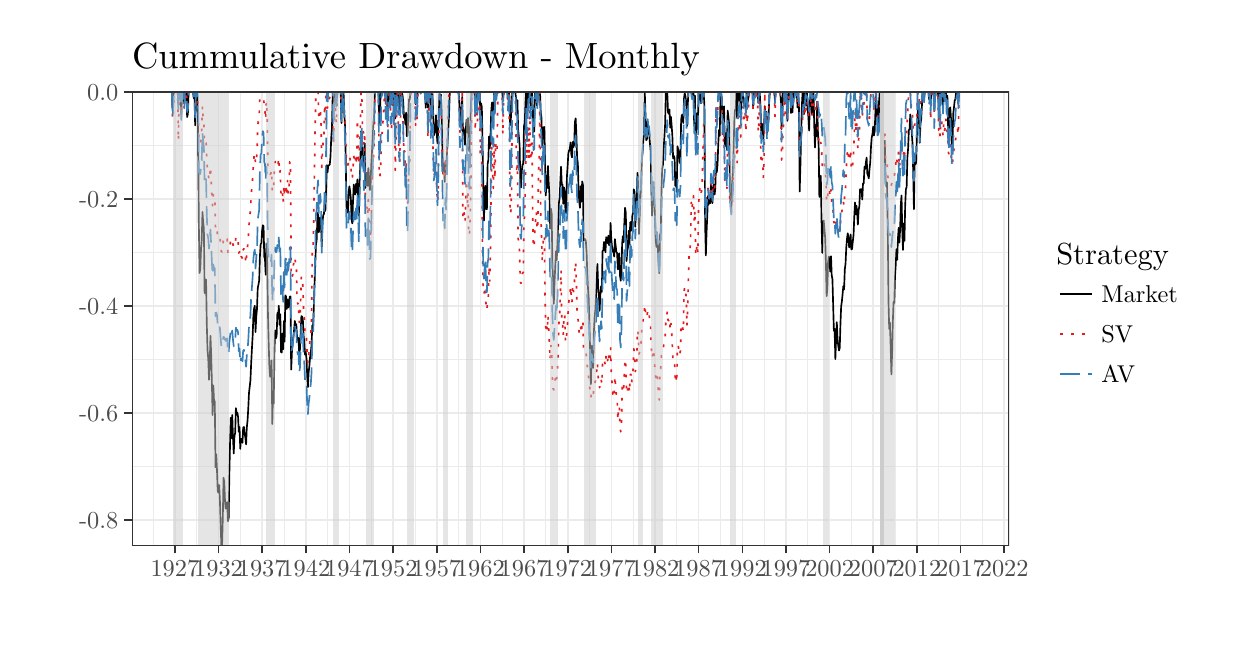
\begin{tikzpicture}[x=1pt,y=1pt]
\definecolor{fillColor}{RGB}{255,255,255}
\path[use as bounding box,fill=fillColor,fill opacity=0.00] (0,0) rectangle (426.79,216.81);
\begin{scope}
\path[clip] (  0.00,  0.00) rectangle (426.79,216.81);
\definecolor{drawColor}{RGB}{255,255,255}
\definecolor{fillColor}{RGB}{255,255,255}

\path[draw=drawColor,line width= 0.6pt,line join=round,line cap=round,fill=fillColor] (  0.00,  0.00) rectangle (426.79,216.81);
\end{scope}
\begin{scope}
\path[clip] ( 37.70, 29.59) rectangle (354.63,193.67);
\definecolor{fillColor}{RGB}{255,255,255}

\path[fill=fillColor] ( 37.70, 29.59) rectangle (354.63,193.67);
\definecolor{drawColor}{gray}{0.92}

\path[draw=drawColor,line width= 0.3pt,line join=round] ( 37.70, 58.23) --
	(354.63, 58.23);

\path[draw=drawColor,line width= 0.3pt,line join=round] ( 37.70, 96.93) --
	(354.63, 96.93);

\path[draw=drawColor,line width= 0.3pt,line join=round] ( 37.70,135.63) --
	(354.63,135.63);

\path[draw=drawColor,line width= 0.3pt,line join=round] ( 37.70,174.33) --
	(354.63,174.33);

\path[draw=drawColor,line width= 0.3pt,line join=round] ( 45.31, 29.59) --
	( 45.31,193.67);

\path[draw=drawColor,line width= 0.3pt,line join=round] ( 61.08, 29.59) --
	( 61.08,193.67);

\path[draw=drawColor,line width= 0.3pt,line join=round] ( 76.85, 29.59) --
	( 76.85,193.67);

\path[draw=drawColor,line width= 0.3pt,line join=round] ( 92.63, 29.59) --
	( 92.63,193.67);

\path[draw=drawColor,line width= 0.3pt,line join=round] (108.40, 29.59) --
	(108.40,193.67);

\path[draw=drawColor,line width= 0.3pt,line join=round] (124.17, 29.59) --
	(124.17,193.67);

\path[draw=drawColor,line width= 0.3pt,line join=round] (139.94, 29.59) --
	(139.94,193.67);

\path[draw=drawColor,line width= 0.3pt,line join=round] (155.72, 29.59) --
	(155.72,193.67);

\path[draw=drawColor,line width= 0.3pt,line join=round] (171.49, 29.59) --
	(171.49,193.67);

\path[draw=drawColor,line width= 0.3pt,line join=round] (187.26, 29.59) --
	(187.26,193.67);

\path[draw=drawColor,line width= 0.3pt,line join=round] (203.03, 29.59) --
	(203.03,193.67);

\path[draw=drawColor,line width= 0.3pt,line join=round] (218.81, 29.59) --
	(218.81,193.67);

\path[draw=drawColor,line width= 0.3pt,line join=round] (234.58, 29.59) --
	(234.58,193.67);

\path[draw=drawColor,line width= 0.3pt,line join=round] (250.35, 29.59) --
	(250.35,193.67);

\path[draw=drawColor,line width= 0.3pt,line join=round] (266.12, 29.59) --
	(266.12,193.67);

\path[draw=drawColor,line width= 0.3pt,line join=round] (281.90, 29.59) --
	(281.90,193.67);

\path[draw=drawColor,line width= 0.3pt,line join=round] (297.67, 29.59) --
	(297.67,193.67);

\path[draw=drawColor,line width= 0.3pt,line join=round] (313.44, 29.59) --
	(313.44,193.67);

\path[draw=drawColor,line width= 0.3pt,line join=round] (329.22, 29.59) --
	(329.22,193.67);

\path[draw=drawColor,line width= 0.3pt,line join=round] (344.99, 29.59) --
	(344.99,193.67);

\path[draw=drawColor,line width= 0.6pt,line join=round] ( 37.70, 38.88) --
	(354.63, 38.88);

\path[draw=drawColor,line width= 0.6pt,line join=round] ( 37.70, 77.58) --
	(354.63, 77.58);

\path[draw=drawColor,line width= 0.6pt,line join=round] ( 37.70,116.28) --
	(354.63,116.28);

\path[draw=drawColor,line width= 0.6pt,line join=round] ( 37.70,154.98) --
	(354.63,154.98);

\path[draw=drawColor,line width= 0.6pt,line join=round] ( 37.70,193.67) --
	(354.63,193.67);

\path[draw=drawColor,line width= 0.6pt,line join=round] ( 53.19, 29.59) --
	( 53.19,193.67);

\path[draw=drawColor,line width= 0.6pt,line join=round] ( 68.96, 29.59) --
	( 68.96,193.67);

\path[draw=drawColor,line width= 0.6pt,line join=round] ( 84.74, 29.59) --
	( 84.74,193.67);

\path[draw=drawColor,line width= 0.6pt,line join=round] (100.51, 29.59) --
	(100.51,193.67);

\path[draw=drawColor,line width= 0.6pt,line join=round] (116.28, 29.59) --
	(116.28,193.67);

\path[draw=drawColor,line width= 0.6pt,line join=round] (132.05, 29.59) --
	(132.05,193.67);

\path[draw=drawColor,line width= 0.6pt,line join=round] (147.83, 29.59) --
	(147.83,193.67);

\path[draw=drawColor,line width= 0.6pt,line join=round] (163.60, 29.59) --
	(163.60,193.67);

\path[draw=drawColor,line width= 0.6pt,line join=round] (179.37, 29.59) --
	(179.37,193.67);

\path[draw=drawColor,line width= 0.6pt,line join=round] (195.15, 29.59) --
	(195.15,193.67);

\path[draw=drawColor,line width= 0.6pt,line join=round] (210.92, 29.59) --
	(210.92,193.67);

\path[draw=drawColor,line width= 0.6pt,line join=round] (226.69, 29.59) --
	(226.69,193.67);

\path[draw=drawColor,line width= 0.6pt,line join=round] (242.46, 29.59) --
	(242.46,193.67);

\path[draw=drawColor,line width= 0.6pt,line join=round] (258.24, 29.59) --
	(258.24,193.67);

\path[draw=drawColor,line width= 0.6pt,line join=round] (274.01, 29.59) --
	(274.01,193.67);

\path[draw=drawColor,line width= 0.6pt,line join=round] (289.78, 29.59) --
	(289.78,193.67);

\path[draw=drawColor,line width= 0.6pt,line join=round] (305.56, 29.59) --
	(305.56,193.67);

\path[draw=drawColor,line width= 0.6pt,line join=round] (321.33, 29.59) --
	(321.33,193.67);

\path[draw=drawColor,line width= 0.6pt,line join=round] (337.10, 29.59) --
	(337.10,193.67);

\path[draw=drawColor,line width= 0.6pt,line join=round] (352.87, 29.59) --
	(352.87,193.67);
\definecolor{drawColor}{RGB}{0,0,0}

\path[draw=drawColor,line width= 0.6pt,line join=round] ( 52.11,193.67) --
	( 52.37,187.60) --
	( 52.63,192.50) --
	( 52.90,193.67) --
	( 53.16,193.54) --
	( 53.43,193.67) --
	( 53.70,193.67) --
	( 53.94,193.67) --
	( 54.20,193.67) --
	( 54.46,189.12) --
	( 54.73,193.67) --
	( 54.99,193.67) --
	( 55.26,193.67) --
	( 55.53,185.27) --
	( 55.79,193.67) --
	( 56.05,193.67) --
	( 56.31,192.62) --
	( 56.58,189.42) --
	( 56.85,193.67) --
	( 57.10,193.67) --
	( 57.37,193.67) --
	( 57.62,184.51) --
	( 57.89,185.65) --
	( 58.15,193.67) --
	( 58.42,193.67) --
	( 58.69,193.67) --
	( 58.95,193.67) --
	( 59.21,193.67) --
	( 59.47,193.67) --
	( 59.74,193.47) --
	( 60.01,191.31) --
	( 60.25,193.67) --
	( 60.52,181.46) --
	( 60.78,193.67) --
	( 61.05,193.67) --
	( 61.30,193.67) --
	( 61.57,183.31) --
	( 61.84,146.70) --
	( 62.10,128.11) --
	( 62.37,129.62) --
	( 62.63,136.67) --
	( 62.89,140.01) --
	( 63.16,150.23) --
	( 63.40,146.71) --
	( 63.67,144.16) --
	( 63.93,120.87) --
	( 64.20,125.61) --
	( 64.46,125.73) --
	( 64.72,109.84) --
	( 64.99,100.26) --
	( 65.25, 97.23) --
	( 65.52, 89.61) --
	( 65.78, 95.19) --
	( 66.05,105.46) --
	( 66.31, 98.70) --
	( 66.56, 88.79) --
	( 66.82, 76.83) --
	( 67.08, 87.52) --
	( 67.35, 81.64) --
	( 67.61, 81.83) --
	( 67.88, 57.97) --
	( 68.14, 62.67) --
	( 68.40, 57.12) --
	( 68.67, 49.39) --
	( 68.93, 48.79) --
	( 69.20, 51.53) --
	( 69.47, 45.75) --
	( 69.72, 37.49) --
	( 69.98, 29.75) --
	( 70.24, 29.59) --
	( 70.51, 39.58) --
	( 70.77, 54.20) --
	( 71.04, 52.64) --
	( 71.31, 45.67) --
	( 71.56, 43.01) --
	( 71.83, 44.94) --
	( 72.09, 45.37) --
	( 72.36, 38.44) --
	( 72.63, 39.70) --
	( 72.87, 55.30) --
	( 73.14, 67.02) --
	( 73.40, 75.86) --
	( 73.66, 68.54) --
	( 73.92, 76.82) --
	( 74.19, 68.69) --
	( 74.46, 62.94) --
	( 74.72, 69.20) --
	( 74.98, 70.43) --
	( 75.24, 79.32) --
	( 75.51, 77.38) --
	( 75.78, 77.68) --
	( 76.02, 76.25) --
	( 76.29, 70.73) --
	( 76.55, 72.51) --
	( 76.82, 64.60) --
	( 77.07, 68.27) --
	( 77.34, 68.10) --
	( 77.61, 66.81) --
	( 77.87, 72.27) --
	( 78.14, 72.52) --
	( 78.40, 70.09) --
	( 78.66, 68.73) --
	( 78.93, 66.25) --
	( 79.17, 72.21) --
	( 79.44, 74.70) --
	( 79.70, 79.00) --
	( 79.97, 84.83) --
	( 80.23, 87.09) --
	( 80.49, 89.35) --
	( 80.76, 95.53) --
	( 81.02,100.56) --
	( 81.29,105.26) --
	( 81.55,112.55) --
	( 81.82,115.39) --
	( 82.08,116.33) --
	( 82.33,106.85) --
	( 82.60,112.38) --
	( 82.86,115.13) --
	( 83.13,122.68) --
	( 83.39,123.99) --
	( 83.66,125.45) --
	( 83.92,134.19) --
	( 84.18,138.58) --
	( 84.45,138.94) --
	( 84.71,143.54) --
	( 84.98,145.42) --
	( 85.24,145.01) --
	( 85.49,134.06) --
	( 85.75,133.10) --
	( 86.01,127.51) --
	( 86.28,138.85) --
	( 86.54,132.11) --
	( 86.81,114.05) --
	( 87.08,103.12) --
	( 87.33, 94.53) --
	( 87.60, 90.67) --
	( 87.86, 91.26) --
	( 88.13, 96.55) --
	( 88.40, 73.57) --
	( 88.64, 84.28) --
	( 88.91, 81.01) --
	( 89.17,100.23) --
	( 89.43,107.44) --
	( 89.69,104.53) --
	( 89.96,105.47) --
	( 90.23,113.78) --
	( 90.49,111.69) --
	( 90.75,116.35) --
	( 91.01,109.40) --
	( 91.28,113.25) --
	( 91.55, 99.61) --
	( 91.79, 99.41) --
	( 92.06,106.27) --
	( 92.32,100.58) --
	( 92.59,110.83) --
	( 92.84,103.38) --
	( 93.11,120.08) --
	( 93.38,119.59) --
	( 93.64,115.14) --
	( 93.91,118.55) --
	( 94.17,115.69) --
	( 94.43,117.39) --
	( 94.70,119.58) --
	( 94.95,119.68) --
	( 95.22, 93.25) --
	( 95.48, 99.48) --
	( 95.75,102.67) --
	( 96.01,105.16) --
	( 96.27,107.57) --
	( 96.54,110.82) --
	( 96.80,108.97) --
	( 97.07,109.68) --
	( 97.33,105.17) --
	( 97.60,103.72) --
	( 97.86,104.72) --
	( 98.10, 99.08) --
	( 98.37,100.37) --
	( 98.63,106.24) --
	( 98.90,112.56) --
	( 99.16,112.43) --
	( 99.43,111.54) --
	( 99.69,105.63) --
	( 99.95,103.49) --
	(100.22, 98.66) --
	(100.48, 99.55) --
	(100.75, 97.19) --
	(101.02, 90.85) --
	(101.26, 86.89) --
	(101.52, 92.10) --
	(101.78, 94.46) --
	(102.05, 97.76) --
	(102.31, 99.53) --
	(102.58,102.19) --
	(102.85,109.21) --
	(103.11,109.30) --
	(103.37,114.87) --
	(103.63,123.25) --
	(103.90,130.65) --
	(104.17,138.67) --
	(104.41,139.64) --
	(104.68,147.57) --
	(104.94,150.08) --
	(105.20,142.88) --
	(105.46,144.75) --
	(105.73,148.19) --
	(106.00,146.43) --
	(106.26,137.63) --
	(106.53,146.42) --
	(106.78,149.01) --
	(107.05,149.48) --
	(107.32,153.13) --
	(107.57,150.56) --
	(107.84,158.19) --
	(108.10,167.12) --
	(108.36,164.53) --
	(108.62,167.05) --
	(108.89,167.07) --
	(109.16,167.37) --
	(109.42,170.13) --
	(109.69,177.05) --
	(109.95,180.58) --
	(110.21,192.17) --
	(110.48,184.59) --
	(110.72,193.67) --
	(110.99,193.67) --
	(111.25,193.67) --
	(111.52,189.35) --
	(111.78,193.67) --
	(112.04,193.67) --
	(112.31,193.67) --
	(112.57,193.67) --
	(112.84,193.67) --
	(113.10,193.67) --
	(113.37,182.35) --
	(113.63,192.84) --
	(113.87,193.67) --
	(114.14,193.67) --
	(114.40,186.14) --
	(114.67,181.19) --
	(114.93,169.47) --
	(115.20,152.15) --
	(115.46,149.96) --
	(115.72,150.02) --
	(115.99,157.48) --
	(116.25,159.49) --
	(116.52,157.68) --
	(116.79,154.99) --
	(117.03,147.56) --
	(117.30,146.10) --
	(117.55,153.82) --
	(117.82,160.12) --
	(118.08,157.30) --
	(118.35,156.52) --
	(118.62,160.35) --
	(118.88,157.26) --
	(119.14,161.98) --
	(119.40,155.76) --
	(119.67,148.88) --
	(119.94,161.06) --
	(120.19,167.07) --
	(120.46,179.32) --
	(120.72,179.12) --
	(120.98,169.99) --
	(121.24,170.47) --
	(121.51,165.26) --
	(121.78,175.06) --
	(122.04,158.90) --
	(122.30,164.00) --
	(122.56,164.44) --
	(122.83,159.64) --
	(123.10,166.09) --
	(123.34,162.97) --
	(123.61,158.17) --
	(123.87,158.37) --
	(124.14,167.12) --
	(124.39,171.45) --
	(124.66,176.78) --
	(124.93,182.23) --
	(125.19,185.44) --
	(125.46,193.67) --
	(125.72,193.67) --
	(125.98,193.67) --
	(126.25,193.67) --
	(126.49,193.67) --
	(126.76,193.67) --
	(127.02,182.28) --
	(127.29,185.04) --
	(127.55,193.67) --
	(127.81,193.67) --
	(128.08,193.25) --
	(128.34,193.67) --
	(128.61,193.67) --
	(128.87,193.67) --
	(129.14,193.67) --
	(129.40,189.34) --
	(129.65,193.67) --
	(129.91,189.12) --
	(130.17,184.06) --
	(130.44,193.67) --
	(130.70,193.67) --
	(130.97,193.67) --
	(131.23,189.05) --
	(131.49,189.99) --
	(131.76,193.67) --
	(132.02,193.67) --
	(132.29,188.58) --
	(132.56,193.67) --
	(132.81,183.94) --
	(133.07,189.77) --
	(133.33,193.67) --
	(133.60,193.67) --
	(133.86,192.08) --
	(134.13,188.13) --
	(134.40,186.85) --
	(134.65,193.67) --
	(134.92,193.67) --
	(135.18,193.16) --
	(135.45,192.50) --
	(135.72,189.73) --
	(135.96,184.22) --
	(136.23,185.16) --
	(136.49,181.84) --
	(136.75,186.09) --
	(137.01,177.58) --
	(137.28,177.84) --
	(137.55,185.97) --
	(137.81,190.96) --
	(138.07,190.84) --
	(138.33,193.67) --
	(138.60,193.67) --
	(138.87,193.67) --
	(139.11,193.67) --
	(139.38,193.67) --
	(139.64,193.67) --
	(139.91,193.67) --
	(140.16,189.16) --
	(140.43,193.67) --
	(140.70,190.44) --
	(140.96,193.67) --
	(141.23,193.67) --
	(141.49,193.67) --
	(141.75,193.67) --
	(142.02,193.33) --
	(142.26,193.67) --
	(142.53,193.67) --
	(142.79,193.67) --
	(143.06,193.67) --
	(143.32,193.67) --
	(143.58,193.09) --
	(143.85,187.83) --
	(144.11,193.67) --
	(144.38,193.67) --
	(144.64,187.91) --
	(144.91,193.67) --
	(145.17,193.67) --
	(145.42,193.67) --
	(145.69,183.86) --
	(145.95,190.34) --
	(146.22,193.67) --
	(146.48,187.53) --
	(146.75,177.85) --
	(147.01,178.84) --
	(147.27,179.35) --
	(147.54,185.15) --
	(147.80,178.85) --
	(148.07,175.09) --
	(148.33,178.83) --
	(148.58,186.45) --
	(148.84,192.84) --
	(149.10,191.39) --
	(149.37,192.60) --
	(149.63,182.53) --
	(149.90,171.51) --
	(150.17,164.04) --
	(150.42,167.80) --
	(150.69,161.07) --
	(150.95,168.57) --
	(151.22,165.78) --
	(151.49,170.88) --
	(151.73,175.93) --
	(152.00,180.09) --
	(152.26,185.25) --
	(152.52,193.33) --
	(152.78,193.67) --
	(153.05,193.67) --
	(153.32,193.67) --
	(153.58,193.67) --
	(153.85,193.67) --
	(154.10,193.67) --
	(154.37,193.67) --
	(154.64,193.67) --
	(154.88,193.67) --
	(155.15,193.67) --
	(155.41,193.42) --
	(155.68,193.67) --
	(155.94,190.79) --
	(156.20,181.76) --
	(156.47,184.27) --
	(156.73,187.11) --
	(157.00,191.78) --
	(157.26,178.62) --
	(157.52,180.58) --
	(157.79,177.68) --
	(158.04,174.47) --
	(158.31,179.78) --
	(158.57,183.53) --
	(158.84,178.89) --
	(159.10,184.20) --
	(159.36,173.18) --
	(159.63,172.07) --
	(159.89,180.14) --
	(160.16,188.46) --
	(160.42,193.67) --
	(160.69,193.67) --
	(160.95,193.67) --
	(161.19,193.67) --
	(161.46,193.67) --
	(161.72,187.84) --
	(161.99,193.12) --
	(162.25,193.67) --
	(162.52,189.47) --
	(162.78,193.67) --
	(163.04,193.67) --
	(163.31,193.45) --
	(163.57,186.18) --
	(163.84,189.45) --
	(164.11,188.11) --
	(164.35,175.84) --
	(164.61,160.65) --
	(164.87,147.07) --
	(165.14,156.31) --
	(165.40,159.65) --
	(165.67,151.24) --
	(165.94,151.22) --
	(166.20,167.51) --
	(166.46,169.07) --
	(166.72,177.47) --
	(166.99,173.19) --
	(167.26,178.44) --
	(167.50,186.46) --
	(167.77,189.76) --
	(168.03,185.88) --
	(168.29,185.12) --
	(168.55,193.67) --
	(168.82,190.86) --
	(169.09,193.67) --
	(169.35,192.08) --
	(169.62,193.67) --
	(169.87,193.67) --
	(170.14,193.67) --
	(170.41,193.67) --
	(170.66,193.67) --
	(170.93,193.67) --
	(171.19,193.67) --
	(171.46,193.67) --
	(171.71,190.92) --
	(171.98,193.67) --
	(172.25,193.67) --
	(172.51,193.67) --
	(172.78,193.67) --
	(173.04,193.67) --
	(173.30,193.67) --
	(173.57,191.26) --
	(173.81,193.67) --
	(174.08,192.14) --
	(174.34,181.62) --
	(174.61,184.09) --
	(174.87,189.11) --
	(175.13,193.67) --
	(175.40,193.67) --
	(175.66,193.67) --
	(175.93,193.67) --
	(176.19,193.67) --
	(176.46,191.38) --
	(176.72,186.67) --
	(176.97,190.63) --
	(177.23,179.94) --
	(177.49,177.49) --
	(177.76,174.49) --
	(178.02,160.74) --
	(178.29,159.06) --
	(178.55,165.11) --
	(178.81,167.33) --
	(179.08,167.61) --
	(179.34,181.21) --
	(179.61,182.46) --
	(179.88,189.56) --
	(180.12,193.67) --
	(180.39,185.35) --
	(180.64,189.72) --
	(180.91,193.67) --
	(181.17,191.94) --
	(181.44,193.67) --
	(181.71,187.79) --
	(181.97,188.66) --
	(182.23,193.67) --
	(182.49,185.98) --
	(182.76,179.14) --
	(183.03,179.34) --
	(183.28,193.67) --
	(183.55,193.67) --
	(183.81,193.67) --
	(184.07,188.57) --
	(184.33,191.14) --
	(184.60,193.67) --
	(184.87,193.67) --
	(185.13,193.67) --
	(185.39,186.30) --
	(185.65,184.28) --
	(185.92,173.66) --
	(186.19,178.01) --
	(186.43,180.83) --
	(186.70,180.91) --
	(186.96,167.84) --
	(187.23,156.16) --
	(187.48,163.36) --
	(187.75,158.84) --
	(188.02,166.83) --
	(188.28,160.48) --
	(188.55,156.38) --
	(188.81,144.19) --
	(189.07,151.39) --
	(189.34,149.78) --
	(189.58,133.20) --
	(189.85,123.93) --
	(190.11,117.03) --
	(190.38,125.03) --
	(190.64,130.53) --
	(190.90,136.01) --
	(191.17,132.84) --
	(191.43,138.78) --
	(191.70,146.53) --
	(191.96,153.43) --
	(192.23,155.37) --
	(192.49,161.71) --
	(192.74,166.55) --
	(193.00,160.01) --
	(193.26,160.06) --
	(193.53,153.18) --
	(193.79,159.09) --
	(194.06,157.66) --
	(194.32,150.55) --
	(194.58,149.81) --
	(194.85,162.86) --
	(195.11,166.86) --
	(195.38,171.45) --
	(195.65,172.45) --
	(195.90,172.96) --
	(196.16,175.32) --
	(196.42,171.16) --
	(196.69,169.93) --
	(196.95,175.52) --
	(197.22,173.64) --
	(197.49,174.64) --
	(197.74,182.70) --
	(198.01,184.02) --
	(198.27,178.31) --
	(198.54,169.78) --
	(198.81,167.71) --
	(199.05,158.39) --
	(199.32,153.81) --
	(199.58,151.69) --
	(199.84,159.51) --
	(200.10,154.00) --
	(200.37,161.26) --
	(200.64,160.08) --
	(200.90,139.83) --
	(201.16,140.51) --
	(201.42,140.35) --
	(201.69,139.78) --
	(201.96,135.67) --
	(202.20,128.69) --
	(202.47,122.61) --
	(202.73,118.91) --
	(203.00,109.68) --
	(203.25, 99.47) --
	(203.52, 87.96) --
	(203.79,101.89) --
	(204.05, 96.93) --
	(204.32, 93.84) --
	(204.58,106.53) --
	(204.84,111.96) --
	(205.11,114.67) --
	(205.35,119.48) --
	(205.62,125.54) --
	(205.88,131.42) --
	(206.15,122.95) --
	(206.41,119.57) --
	(206.67,114.48) --
	(206.94,120.29) --
	(207.20,123.39) --
	(207.47,121.36) --
	(207.73,136.07) --
	(208.00,136.41) --
	(208.26,139.40) --
	(208.51,137.49) --
	(208.78,135.66) --
	(209.04,141.10) --
	(209.31,139.71) --
	(209.57,138.92) --
	(209.84,141.65) --
	(210.10,138.19) --
	(210.36,138.32) --
	(210.63,146.23) --
	(210.89,140.36) --
	(211.16,137.60) --
	(211.43,135.84) --
	(211.67,136.04) --
	(211.93,134.07) --
	(212.19,140.41) --
	(212.46,138.10) --
	(212.72,135.72) --
	(212.99,135.37) --
	(213.26,129.49) --
	(213.52,134.78) --
	(213.78,135.23) --
	(214.04,127.14) --
	(214.31,125.35) --
	(214.58,128.97) --
	(214.82,139.01) --
	(215.09,141.48) --
	(215.35,139.21) --
	(215.61,146.36) --
	(215.87,151.73) --
	(216.14,149.85) --
	(216.41,132.49) --
	(216.67,136.12) --
	(216.94,137.59) --
	(217.19,143.39) --
	(217.46,138.48) --
	(217.73,146.43) --
	(217.97,146.60) --
	(218.24,143.46) --
	(218.50,148.98) --
	(218.77,149.98) --
	(219.03,158.40) --
	(219.29,157.41) --
	(219.56,144.87) --
	(219.82,152.81) --
	(220.09,155.76) --
	(220.35,164.34) --
	(220.61,162.96) --
	(220.88,142.26) --
	(221.13,148.37) --
	(221.40,155.39) --
	(221.66,159.24) --
	(221.93,168.92) --
	(222.19,171.85) --
	(222.45,175.98) --
	(222.72,178.37) --
	(222.98,193.67) --
	(223.25,185.26) --
	(223.51,176.15) --
	(223.78,176.57) --
	(224.04,182.82) --
	(224.28,178.85) --
	(224.55,179.10) --
	(224.81,175.38) --
	(225.08,172.85) --
	(225.34,160.97) --
	(225.61,148.87) --
	(225.87,155.82) --
	(226.13,160.96) --
	(226.40,154.58) --
	(226.66,148.94) --
	(226.93,140.12) --
	(227.20,137.60) --
	(227.44,142.24) --
	(227.71,136.90) --
	(227.96,132.14) --
	(228.23,128.07) --
	(228.49,141.93) --
	(228.76,142.81) --
	(229.03,158.53) --
	(229.29,165.90) --
	(229.55,167.32) --
	(229.81,173.23) --
	(230.08,177.27) --
	(230.35,182.16) --
	(230.59,193.67) --
	(230.86,193.67) --
	(231.12,193.67) --
	(231.38,186.28) --
	(231.64,185.68) --
	(231.91,187.28) --
	(232.18,180.65) --
	(232.44,184.59) --
	(232.71,181.28) --
	(232.96,177.68) --
	(233.23,169.51) --
	(233.50,170.48) --
	(233.75,169.71) --
	(234.02,159.67) --
	(234.28,162.09) --
	(234.55,157.52) --
	(234.80,173.95) --
	(235.07,172.61) --
	(235.34,171.18) --
	(235.60,167.91) --
	(235.87,170.17) --
	(236.13,183.41) --
	(236.39,185.32) --
	(236.66,183.80) --
	(236.90,182.34) --
	(237.17,191.32) --
	(237.43,193.20) --
	(237.70,191.88) --
	(237.96,189.92) --
	(238.22,181.24) --
	(238.49,188.25) --
	(238.75,193.67) --
	(239.02,193.67) --
	(239.28,193.67) --
	(239.55,193.67) --
	(239.81,193.67) --
	(240.06,191.13) --
	(240.32,193.67) --
	(240.58,193.67) --
	(240.85,181.24) --
	(241.11,192.22) --
	(241.38,176.13) --
	(241.64,183.96) --
	(241.90,185.90) --
	(242.17,180.17) --
	(242.43,193.67) --
	(242.70,193.67) --
	(242.97,193.67) --
	(243.21,189.57) --
	(243.48,189.65) --
	(243.73,193.67) --
	(244.00,193.67) --
	(244.26,193.67) --
	(244.53,188.79) --
	(244.80,145.60) --
	(245.06,134.49) --
	(245.32,143.07) --
	(245.58,148.97) --
	(245.85,156.05) --
	(246.12,153.02) --
	(246.37,153.99) --
	(246.64,153.39) --
	(246.90,160.53) --
	(247.16,158.56) --
	(247.42,153.37) --
	(247.69,158.26) --
	(247.96,160.11) --
	(248.22,156.52) --
	(248.48,158.84) --
	(248.74,168.37) --
	(249.01,164.57) --
	(249.28,167.18) --
	(249.52,174.17) --
	(249.79,179.81) --
	(250.05,177.75) --
	(250.32,189.94) --
	(250.57,192.78) --
	(250.84,191.15) --
	(251.11,184.20) --
	(251.37,186.27) --
	(251.64,188.39) --
	(251.90,174.00) --
	(252.16,175.52) --
	(252.43,178.73) --
	(252.67,172.70) --
	(252.94,186.85) --
	(253.20,184.79) --
	(253.47,181.82) --
	(253.73,164.09) --
	(253.99,154.22) --
	(254.26,151.30) --
	(254.52,160.27) --
	(254.79,163.88) --
	(255.05,170.94) --
	(255.32,182.80) --
	(255.58,187.11) --
	(255.83,186.83) --
	(256.09,193.58) --
	(256.35,184.09) --
	(256.62,191.80) --
	(256.88,193.67) --
	(257.15,190.62) --
	(257.41,193.12) --
	(257.67,185.08) --
	(257.94,193.67) --
	(258.20,192.70) --
	(258.47,193.67) --
	(258.74,188.45) --
	(258.99,190.44) --
	(259.25,191.02) --
	(259.51,186.74) --
	(259.78,193.65) --
	(260.04,189.01) --
	(260.31,190.77) --
	(260.58,192.37) --
	(260.83,193.67) --
	(261.10,193.67) --
	(261.36,193.67) --
	(261.63,193.67) --
	(261.90,193.67) --
	(262.14,188.35) --
	(262.41,193.43) --
	(262.67,193.67) --
	(262.93,193.10) --
	(263.19,193.67) --
	(263.46,193.34) --
	(263.73,193.67) --
	(263.99,189.78) --
	(264.26,193.05) --
	(264.51,193.67) --
	(264.78,188.55) --
	(265.05,179.48) --
	(265.29,180.80) --
	(265.56,182.00) --
	(265.82,176.45) --
	(266.09,181.29) --
	(266.35,188.42) --
	(266.61,184.45) --
	(266.88,186.43) --
	(267.14,178.84) --
	(267.41,180.41) --
	(267.67,183.41) --
	(267.93,189.83) --
	(268.20,193.67) --
	(268.44,193.67) --
	(268.71,193.67) --
	(268.97,193.67) --
	(269.24,193.67) --
	(269.50,193.67) --
	(269.77,193.67) --
	(270.03,190.59) --
	(270.29,193.67) --
	(270.56,193.67) --
	(270.82,193.67) --
	(271.09,193.67) --
	(271.35,193.67) --
	(271.60,193.67) --
	(271.87,193.67) --
	(272.13,191.19) --
	(272.40,180.16) --
	(272.66,185.25) --
	(272.93,193.67) --
	(273.19,193.67) --
	(273.45,193.67) --
	(273.72,190.67) --
	(273.98,193.67) --
	(274.25,192.57) --
	(274.52,183.12) --
	(274.76,190.13) --
	(275.02,193.67) --
	(275.28,193.67) --
	(275.55,193.67) --
	(275.81,185.97) --
	(276.08,193.67) --
	(276.35,186.25) --
	(276.61,191.07) --
	(276.87,193.65) --
	(277.13,193.67) --
	(277.40,193.67) --
	(277.67,193.67) --
	(277.91,193.67) --
	(278.18,187.96) --
	(278.44,193.13) --
	(278.70,187.87) --
	(278.96,157.60) --
	(279.23,166.98) --
	(279.50,178.62) --
	(279.76,188.82) --
	(280.03,193.67) --
	(280.28,193.67) --
	(280.55,185.60) --
	(280.82,191.96) --
	(281.06,193.67) --
	(281.33,188.86) --
	(281.59,193.67) --
	(281.86,187.10) --
	(282.12,184.49) --
	(282.38,179.60) --
	(282.65,190.01) --
	(282.91,193.67) --
	(283.18,193.67) --
	(283.44,185.34) --
	(283.70,190.39) --
	(283.97,193.67) --
	(284.22,181.38) --
	(284.49,173.52) --
	(284.75,181.63) --
	(285.02,177.53) --
	(285.28,190.07) --
	(285.54,179.50) --
	(285.81,174.24) --
	(286.07,155.63) --
	(286.34,157.92) --
	(286.60,163.33) --
	(286.87,146.43) --
	(287.13,135.41) --
	(287.38,146.19) --
	(287.64,147.10) --
	(287.90,143.96) --
	(288.17,140.88) --
	(288.43,132.21) --
	(288.70,119.77) --
	(288.96,122.72) --
	(289.22,132.00) --
	(289.49,134.06) --
	(289.75,131.70) --
	(290.02,128.65) --
	(290.29,134.21) --
	(290.53,127.39) --
	(290.80,125.89) --
	(291.05,116.88) --
	(291.32,107.26) --
	(291.58,107.98) --
	(291.85, 97.06) --
	(292.12,104.17) --
	(292.38,110.39) --
	(292.64,104.37) --
	(292.90,101.81) --
	(293.17,100.14) --
	(293.44,101.07) --
	(293.68,109.32) --
	(293.95,116.13) --
	(294.21,117.91) --
	(294.47,120.52) --
	(294.73,123.40) --
	(295.00,122.19) --
	(295.27,129.46) --
	(295.53,131.50) --
	(295.80,137.38) --
	(296.05,140.44) --
	(296.32,142.50) --
	(296.59,140.88) --
	(296.84,137.39) --
	(297.11,139.19) --
	(297.37,142.08) --
	(297.64,136.66) --
	(297.89,136.92) --
	(298.16,139.59) --
	(298.43,141.91) --
	(298.69,148.58) --
	(298.96,153.63) --
	(299.22,149.33) --
	(299.48,152.47) --
	(299.75,149.65) --
	(299.99,145.66) --
	(300.26,150.86) --
	(300.52,152.28) --
	(300.79,158.49) --
	(301.05,157.19) --
	(301.31,158.47) --
	(301.58,154.70) --
	(301.84,160.47) --
	(302.11,160.59) --
	(302.37,166.50) --
	(302.64,165.70) --
	(302.90,168.26) --
	(303.15,169.87) --
	(303.41,163.99) --
	(303.67,163.34) --
	(303.94,162.34) --
	(304.20,165.74) --
	(304.47,168.28) --
	(304.73,173.79) --
	(304.99,177.18) --
	(305.26,178.37) --
	(305.52,181.07) --
	(305.79,177.83) --
	(306.06,179.34) --
	(306.30,185.77) --
	(306.57,192.17) --
	(306.82,188.51) --
	(307.09,181.78) --
	(307.35,183.16) --
	(307.62,189.88) --
	(307.89,193.67) --
	(308.15,183.54) --
	(308.41,182.15) --
	(308.67,170.26) --
	(308.94,166.13) --
	(309.21,164.06) --
	(309.46,172.21) --
	(309.73,176.01) --
	(309.99,161.93) --
	(310.25,159.49) --
	(310.51,160.90) --
	(310.78,144.93) --
	(311.05,118.05) --
	(311.31,107.92) --
	(311.57,110.21) --
	(311.83,101.68) --
	(312.10, 91.50) --
	(312.37, 99.42) --
	(312.61,110.26) --
	(312.88,117.70) --
	(313.14,117.33) --
	(313.41,126.90) --
	(313.66,130.87) --
	(313.93,136.77) --
	(314.20,132.93) --
	(314.46,140.50) --
	(314.73,144.48) --
	(314.99,139.13) --
	(315.25,143.95) --
	(315.52,153.09) --
	(315.76,156.16) --
	(316.03,143.80) --
	(316.29,136.50) --
	(316.56,146.07) --
	(316.82,139.81) --
	(317.08,152.57) --
	(317.35,158.43) --
	(317.61,159.22) --
	(317.88,169.88) --
	(318.14,173.12) --
	(318.41,179.70) --
	(318.67,180.29) --
	(318.92,185.43) --
	(319.18,182.65) --
	(319.44,179.29) --
	(319.71,175.27) --
	(319.97,165.21) --
	(320.24,151.20) --
	(320.51,168.40) --
	(320.76,167.35) --
	(321.03,167.97) --
	(321.29,177.04) --
	(321.56,184.32) --
	(321.83,188.74) --
	(322.08,187.46) --
	(322.34,175.19) --
	(322.60,181.87) --
	(322.87,183.71) --
	(323.13,188.53) --
	(323.40,193.53) --
	(323.67,190.79) --
	(323.93,191.95) --
	(324.19,193.67) --
	(324.45,193.67) --
	(324.72,193.67) --
	(324.99,193.67) --
	(325.23,193.67) --
	(325.50,193.67) --
	(325.76,190.76) --
	(326.02,193.67) --
	(326.28,188.70) --
	(326.55,193.67) --
	(326.82,193.67) --
	(327.08,193.67) --
	(327.35,193.67) --
	(327.60,187.88) --
	(327.87,193.67) --
	(328.14,193.67) --
	(328.38,193.67) --
	(328.65,193.67) --
	(328.91,193.67) --
	(329.18,189.70) --
	(329.44,193.67) --
	(329.70,188.81) --
	(329.97,192.81) --
	(330.23,193.67) --
	(330.50,192.98) --
	(330.76,187.74) --
	(331.02,193.67) --
	(331.29,191.65) --
	(331.53,193.33) --
	(331.80,193.67) --
	(332.06,189.95) --
	(332.33,192.24) --
	(332.59,180.72) --
	(332.86,174.63) --
	(333.12,187.53) --
	(333.38,187.99) --
	(333.65,183.81) --
	(333.91,173.34) --
	(334.18,173.44) --
	(334.44,185.63) --
	(334.69,187.78) --
	(334.96,190.42) --
	(335.22,191.00) --
	(335.49,193.67) --
	(335.75,193.67) --
	(336.02,193.67) --
	(336.28,189.46) --
	(336.54,193.67) --
	(336.81,193.67) --
	(337.07,193.67) --
	(337.34,193.67) --
	(337.61,193.67) --
	(337.85,193.67) --
	(338.12,193.67) --
	(338.37,193.67) --
	(338.64,193.67) --
	(338.90,193.67) --
	(339.17,193.67) --
	(339.44,193.67) --
	(339.70,193.67) --
	(339.96,193.67) --
	(340.22,193.67);
\definecolor{drawColor}{RGB}{228,26,28}

\path[draw=drawColor,line width= 0.6pt,dash pattern=on 1pt off 3pt ,line join=round] ( 52.11,193.67) --
	( 52.37,183.67) --
	( 52.63,186.35) --
	( 52.90,193.67) --
	( 53.16,193.37) --
	( 53.43,193.67) --
	( 53.70,193.67) --
	( 53.94,193.67) --
	( 54.20,193.67) --
	( 54.46,175.98) --
	( 54.73,191.84) --
	( 54.99,193.67) --
	( 55.26,193.67) --
	( 55.53,185.05) --
	( 55.79,193.67) --
	( 56.05,193.67) --
	( 56.31,191.71) --
	( 56.58,188.01) --
	( 56.85,193.67) --
	( 57.10,193.67) --
	( 57.37,193.67) --
	( 57.62,188.55) --
	( 57.89,188.82) --
	( 58.15,193.67) --
	( 58.42,193.67) --
	( 58.69,193.67) --
	( 58.95,193.67) --
	( 59.21,193.67) --
	( 59.47,193.67) --
	( 59.74,193.53) --
	( 60.01,192.78) --
	( 60.25,193.38) --
	( 60.52,187.41) --
	( 60.78,191.92) --
	( 61.05,193.67) --
	( 61.30,193.67) --
	( 61.57,190.10) --
	( 61.84,175.35) --
	( 62.10,174.96) --
	( 62.37,175.02) --
	( 62.63,176.01) --
	( 62.89,180.06) --
	( 63.16,188.55) --
	( 63.40,184.08) --
	( 63.67,182.01) --
	( 63.93,175.07) --
	( 64.20,175.63) --
	( 64.46,175.67) --
	( 64.72,169.60) --
	( 64.99,164.27) --
	( 65.25,163.80) --
	( 65.52,161.72) --
	( 65.78,163.05) --
	( 66.05,166.58) --
	( 66.31,161.37) --
	( 66.56,156.32) --
	( 66.82,152.47) --
	( 67.08,156.50) --
	( 67.35,155.90) --
	( 67.61,155.96) --
	( 67.88,143.21) --
	( 68.14,143.91) --
	( 68.40,143.54) --
	( 68.67,141.42) --
	( 68.93,141.33) --
	( 69.20,141.84) --
	( 69.47,141.08) --
	( 69.72,138.31) --
	( 69.98,135.88) --
	( 70.24,135.83) --
	( 70.51,137.47) --
	( 70.77,140.95) --
	( 71.04,140.79) --
	( 71.31,140.25) --
	( 71.56,139.97) --
	( 71.83,140.28) --
	( 72.09,140.45) --
	( 72.36,135.58) --
	( 72.63,135.99) --
	( 72.87,137.28) --
	( 73.14,138.51) --
	( 73.40,140.15) --
	( 73.66,139.42) --
	( 73.92,139.89) --
	( 74.19,138.43) --
	( 74.46,137.46) --
	( 74.72,138.02) --
	( 74.98,138.32) --
	( 75.24,141.32) --
	( 75.51,140.71) --
	( 75.78,140.82) --
	( 76.02,140.35) --
	( 76.29,135.35) --
	( 76.55,135.87) --
	( 76.82,133.24) --
	( 77.07,134.02) --
	( 77.34,133.96) --
	( 77.61,133.32) --
	( 77.87,136.58) --
	( 78.14,136.95) --
	( 78.40,134.95) --
	( 78.66,133.63) --
	( 78.93,131.64) --
	( 79.17,135.48) --
	( 79.44,137.59) --
	( 79.70,140.63) --
	( 79.97,145.29) --
	( 80.23,148.94) --
	( 80.49,150.48) --
	( 80.76,156.13) --
	( 81.02,159.31) --
	( 81.29,162.27) --
	( 81.55,167.46) --
	( 81.82,170.48) --
	( 82.08,171.29) --
	( 82.33,167.63) --
	( 82.60,169.48) --
	( 82.86,171.17) --
	( 83.13,181.37) --
	( 83.39,183.30) --
	( 83.66,184.46) --
	( 83.92,193.67) --
	( 84.18,193.67) --
	( 84.45,193.67) --
	( 84.71,193.67) --
	( 84.98,193.67) --
	( 85.24,193.13) --
	( 85.49,186.76) --
	( 85.75,186.48) --
	( 86.01,183.63) --
	( 86.28,190.18) --
	( 86.54,184.95) --
	( 86.81,165.93) --
	( 87.08,164.75) --
	( 87.33,164.26) --
	( 87.60,163.86) --
	( 87.86,164.05) --
	( 88.13,165.32) --
	( 88.40,157.93) --
	( 88.64,160.10) --
	( 88.91,159.66) --
	( 89.17,166.92) --
	( 89.43,168.44) --
	( 89.69,167.55) --
	( 89.96,167.88) --
	( 90.23,168.77) --
	( 90.49,167.66) --
	( 90.75,169.75) --
	( 91.01,164.16) --
	( 91.28,165.17) --
	( 91.55,155.82) --
	( 91.79,155.78) --
	( 92.06,157.18) --
	( 92.32,153.46) --
	( 92.59,159.93) --
	( 92.84,155.82) --
	( 93.11,160.18) --
	( 93.38,160.13) --
	( 93.64,156.04) --
	( 93.91,161.53) --
	( 94.17,156.70) --
	( 94.43,158.69) --
	( 94.70,168.31) --
	( 94.95,168.55) --
	( 95.22,126.33) --
	( 95.48,126.81) --
	( 95.75,127.34) --
	( 96.01,131.08) --
	( 96.27,132.25) --
	( 96.54,133.86) --
	( 96.80,131.62) --
	( 97.07,131.81) --
	( 97.33,118.40) --
	( 97.60,116.97) --
	( 97.86,117.50) --
	( 98.10,110.28) --
	( 98.37,111.35) --
	( 98.63,118.10) --
	( 98.90,126.94) --
	( 99.16,126.77) --
	( 99.43,123.51) --
	( 99.69,115.03) --
	( 99.95,112.69) --
	(100.22,105.95) --
	(100.48,106.11) --
	(100.75,104.66) --
	(101.02, 97.62) --
	(101.26, 95.62) --
	(101.52, 98.30) --
	(101.78,100.78) --
	(102.05,104.00) --
	(102.31,105.35) --
	(102.58,112.35) --
	(102.85,137.41) --
	(103.11,137.53) --
	(103.37,147.50) --
	(103.63,165.15) --
	(103.90,183.09) --
	(104.17,193.67) --
	(104.41,193.67) --
	(104.68,193.67) --
	(104.94,193.67) --
	(105.20,183.39) --
	(105.46,184.52) --
	(105.73,187.62) --
	(106.00,183.14) --
	(106.26,166.31) --
	(106.53,171.84) --
	(106.78,175.82) --
	(107.05,176.90) --
	(107.32,189.06) --
	(107.57,183.58) --
	(107.84,193.67) --
	(108.10,193.67) --
	(108.36,187.75) --
	(108.62,191.04) --
	(108.89,191.11) --
	(109.16,191.44) --
	(109.42,193.67) --
	(109.69,193.67) --
	(109.95,193.67) --
	(110.21,193.67) --
	(110.48,174.37) --
	(110.72,182.07) --
	(110.99,186.41) --
	(111.25,187.54) --
	(111.52,182.09) --
	(111.78,189.10) --
	(112.04,193.67) --
	(112.31,193.67) --
	(112.57,193.67) --
	(112.84,193.67) --
	(113.10,193.67) --
	(113.37,188.33) --
	(113.63,190.18) --
	(113.87,193.67) --
	(114.14,193.67) --
	(114.40,186.57) --
	(114.67,183.12) --
	(114.93,176.62) --
	(115.20,167.29) --
	(115.46,167.13) --
	(115.72,167.14) --
	(115.99,169.43) --
	(116.25,170.33) --
	(116.52,169.26) --
	(116.79,166.75) --
	(117.03,163.05) --
	(117.30,162.27) --
	(117.55,166.11) --
	(117.82,170.58) --
	(118.08,168.75) --
	(118.35,167.70) --
	(118.62,171.13) --
	(118.88,167.28) --
	(119.14,183.68) --
	(119.40,175.36) --
	(119.67,167.37) --
	(119.94,175.53) --
	(120.19,179.60) --
	(120.46,193.67) --
	(120.72,193.44) --
	(120.98,180.94) --
	(121.24,181.16) --
	(121.51,174.08) --
	(121.78,178.88) --
	(122.04,151.42) --
	(122.30,152.31) --
	(122.56,152.85) --
	(122.83,148.99) --
	(123.10,154.69) --
	(123.34,151.48) --
	(123.61,140.79) --
	(123.87,141.03) --
	(124.14,146.39) --
	(124.39,159.21) --
	(124.66,165.53) --
	(124.93,169.06) --
	(125.19,174.52) --
	(125.46,190.64) --
	(125.72,193.67) --
	(125.98,193.67) --
	(126.25,193.67) --
	(126.49,193.67) --
	(126.76,193.67) --
	(127.02,162.86) --
	(127.29,163.32) --
	(127.55,165.88) --
	(127.81,179.01) --
	(128.08,178.58) --
	(128.34,182.36) --
	(128.61,186.52) --
	(128.87,190.94) --
	(129.14,192.77) --
	(129.40,184.33) --
	(129.65,191.59) --
	(129.91,185.78) --
	(130.17,181.01) --
	(130.44,193.67) --
	(130.70,193.67) --
	(130.97,193.67) --
	(131.23,180.21) --
	(131.49,180.79) --
	(131.76,188.18) --
	(132.02,193.67) --
	(132.29,180.90) --
	(132.56,190.59) --
	(132.81,165.28) --
	(133.07,173.79) --
	(133.33,189.54) --
	(133.60,193.67) --
	(133.86,186.66) --
	(134.13,170.73) --
	(134.40,167.65) --
	(134.65,179.25) --
	(134.92,193.67) --
	(135.18,189.65) --
	(135.45,187.60) --
	(135.72,179.26) --
	(135.96,171.42) --
	(136.23,172.29) --
	(136.49,165.36) --
	(136.75,168.80) --
	(137.01,152.50) --
	(137.28,152.91) --
	(137.55,158.79) --
	(137.81,168.97) --
	(138.07,168.59) --
	(138.33,192.49) --
	(138.60,193.67) --
	(138.87,193.67) --
	(139.11,193.67) --
	(139.38,193.67) --
	(139.64,193.67) --
	(139.91,193.67) --
	(140.16,180.82) --
	(140.43,193.67) --
	(140.70,182.93) --
	(140.96,193.67) --
	(141.23,193.67) --
	(141.49,193.67) --
	(141.75,193.67) --
	(142.02,192.91) --
	(142.26,193.67) --
	(142.53,193.67) --
	(142.79,193.67) --
	(143.06,193.67) --
	(143.32,193.67) --
	(143.58,192.94) --
	(143.85,191.99) --
	(144.11,193.67) --
	(144.38,193.67) --
	(144.64,176.77) --
	(144.91,183.01) --
	(145.17,193.67) --
	(145.42,193.67) --
	(145.69,181.13) --
	(145.95,185.14) --
	(146.22,193.67) --
	(146.48,171.63) --
	(146.75,162.79) --
	(147.01,164.26) --
	(147.27,164.60) --
	(147.54,168.17) --
	(147.80,158.92) --
	(148.07,153.74) --
	(148.33,156.77) --
	(148.58,178.99) --
	(148.84,193.67) --
	(149.10,190.04) --
	(149.37,192.08) --
	(149.63,174.39) --
	(149.90,169.19) --
	(150.17,163.95) --
	(150.42,164.65) --
	(150.69,162.81) --
	(150.95,168.90) --
	(151.22,165.08) --
	(151.49,172.30) --
	(151.73,182.97) --
	(152.00,189.14) --
	(152.26,193.67) --
	(152.52,193.67) --
	(152.78,193.67) --
	(153.05,193.67) --
	(153.32,193.67) --
	(153.58,193.67) --
	(153.85,193.67) --
	(154.10,193.67) --
	(154.37,193.67) --
	(154.64,193.67) --
	(154.88,193.67) --
	(155.15,193.67) --
	(155.41,193.09) --
	(155.68,193.67) --
	(155.94,187.00) --
	(156.20,179.04) --
	(156.47,180.46) --
	(156.73,184.90) --
	(157.00,193.67) --
	(157.26,148.91) --
	(157.52,151.39) --
	(157.79,149.28) --
	(158.04,146.60) --
	(158.31,153.84) --
	(158.57,161.62) --
	(158.84,152.83) --
	(159.10,157.20) --
	(159.36,142.24) --
	(159.63,141.71) --
	(159.89,147.52) --
	(160.16,159.21) --
	(160.42,190.51) --
	(160.69,193.67) --
	(160.95,193.67) --
	(161.19,193.67) --
	(161.46,193.67) --
	(161.72,179.49) --
	(161.99,189.28) --
	(162.25,193.67) --
	(162.52,182.52) --
	(162.78,188.19) --
	(163.04,193.67) --
	(163.31,192.86) --
	(163.57,170.84) --
	(163.84,174.82) --
	(164.11,169.94) --
	(164.35,134.32) --
	(164.61,121.56) --
	(164.87,120.60) --
	(165.14,121.77) --
	(165.40,123.25) --
	(165.67,114.83) --
	(165.94,114.81) --
	(166.20,118.36) --
	(166.46,119.71) --
	(166.72,130.65) --
	(166.99,125.27) --
	(167.26,136.60) --
	(167.50,159.85) --
	(167.77,176.17) --
	(168.03,161.61) --
	(168.29,158.73) --
	(168.55,175.00) --
	(168.82,162.16) --
	(169.09,175.43) --
	(169.35,171.89) --
	(169.62,172.87) --
	(169.87,191.06) --
	(170.14,193.67) --
	(170.41,193.67) --
	(170.66,193.67) --
	(170.93,193.67) --
	(171.19,193.67) --
	(171.46,193.67) --
	(171.71,178.13) --
	(171.98,191.17) --
	(172.25,193.67) --
	(172.51,193.67) --
	(172.78,193.67) --
	(173.04,193.67) --
	(173.30,193.67) --
	(173.57,187.18) --
	(173.81,193.67) --
	(174.08,178.83) --
	(174.34,149.46) --
	(174.61,150.52) --
	(174.87,158.52) --
	(175.13,193.67) --
	(175.40,193.67) --
	(175.66,193.63) --
	(175.93,193.67) --
	(176.19,193.67) --
	(176.46,177.43) --
	(176.72,164.21) --
	(176.97,167.51) --
	(177.23,140.52) --
	(177.49,139.59) --
	(177.76,135.36) --
	(178.02,124.86) --
	(178.29,124.43) --
	(178.55,127.36) --
	(178.81,128.05) --
	(179.08,128.32) --
	(179.34,146.87) --
	(179.61,149.05) --
	(179.88,162.69) --
	(180.12,179.21) --
	(180.39,169.21) --
	(180.64,174.26) --
	(180.91,181.19) --
	(181.17,169.23) --
	(181.44,187.32) --
	(181.71,168.64) --
	(181.97,170.59) --
	(182.23,175.16) --
	(182.49,148.27) --
	(182.76,137.39) --
	(183.03,137.55) --
	(183.28,144.74) --
	(183.55,147.41) --
	(183.81,150.31) --
	(184.07,143.79) --
	(184.33,145.93) --
	(184.60,165.48) --
	(184.87,170.27) --
	(185.13,193.67) --
	(185.39,149.11) --
	(185.65,143.18) --
	(185.92,132.33) --
	(186.19,138.01) --
	(186.43,141.72) --
	(186.70,141.82) --
	(186.96,119.36) --
	(187.23,108.24) --
	(187.48,110.11) --
	(187.75,107.16) --
	(188.02,112.89) --
	(188.28,107.52) --
	(188.55,102.56) --
	(188.81, 96.84) --
	(189.07,101.94) --
	(189.34,100.83) --
	(189.58, 90.63) --
	(189.85, 86.46) --
	(190.11, 85.95) --
	(190.38, 87.89) --
	(190.64, 89.83) --
	(190.90, 91.76) --
	(191.17, 89.95) --
	(191.43, 93.64) --
	(191.70, 99.24) --
	(191.96,109.97) --
	(192.23,112.90) --
	(192.49,121.18) --
	(192.74,129.31) --
	(193.00,110.20) --
	(193.26,110.26) --
	(193.53,105.59) --
	(193.79,113.25) --
	(194.06,112.87) --
	(194.32,103.91) --
	(194.58,103.14) --
	(194.85,107.36) --
	(195.11,110.36) --
	(195.38,115.95) --
	(195.65,118.80) --
	(195.90,119.37) --
	(196.16,123.29) --
	(196.42,119.94) --
	(196.69,117.47) --
	(196.95,123.82) --
	(197.22,121.42) --
	(197.49,122.81) --
	(197.74,129.52) --
	(198.01,132.17) --
	(198.27,124.13) --
	(198.54,113.77) --
	(198.81,112.61) --
	(199.05,108.62) --
	(199.32,106.43) --
	(199.58,105.99) --
	(199.84,108.54) --
	(200.10,106.39) --
	(200.37,111.08) --
	(200.64,110.03) --
	(200.90, 99.54) --
	(201.16, 99.66) --
	(201.42, 99.64) --
	(201.69, 99.51) --
	(201.96, 97.82) --
	(202.20, 94.59) --
	(202.47, 91.91) --
	(202.73, 90.48) --
	(203.00, 87.41) --
	(203.25, 85.68) --
	(203.52, 83.20) --
	(203.79, 84.94) --
	(204.05, 84.43) --
	(204.32, 83.61) --
	(204.58, 86.52) --
	(204.84, 87.86) --
	(205.11, 88.99) --
	(205.35, 90.59) --
	(205.62, 92.94) --
	(205.88, 95.72) --
	(206.15, 90.47) --
	(206.41, 88.26) --
	(206.67, 86.71) --
	(206.94, 88.67) --
	(207.20, 89.90) --
	(207.47, 87.96) --
	(207.73, 95.25) --
	(208.00, 95.44) --
	(208.26, 97.15) --
	(208.51, 95.94) --
	(208.78, 94.69) --
	(209.04, 98.97) --
	(209.31, 97.74) --
	(209.57, 96.48) --
	(209.84, 99.27) --
	(210.10, 95.99) --
	(210.36, 96.07) --
	(210.63,101.35) --
	(210.89, 91.81) --
	(211.16, 88.28) --
	(211.43, 84.41) --
	(211.67, 84.62) --
	(211.93, 83.30) --
	(212.19, 90.90) --
	(212.46, 87.07) --
	(212.72, 84.23) --
	(212.99, 83.73) --
	(213.26, 75.01) --
	(213.52, 79.89) --
	(213.78, 80.10) --
	(214.04, 72.16) --
	(214.31, 70.79) --
	(214.58, 74.57) --
	(214.82, 86.97) --
	(215.09, 88.33) --
	(215.35, 86.68) --
	(215.61, 91.62) --
	(215.87, 97.03) --
	(216.14, 95.67) --
	(216.41, 84.61) --
	(216.67, 85.81) --
	(216.94, 86.07) --
	(217.19, 88.17) --
	(217.46, 84.94) --
	(217.73, 91.38) --
	(217.97, 91.56) --
	(218.24, 88.39) --
	(218.50, 91.96) --
	(218.77, 93.28) --
	(219.03,100.78) --
	(219.29, 98.97) --
	(219.56, 92.56) --
	(219.82, 94.15) --
	(220.09, 95.39) --
	(220.35,107.52) --
	(220.61,107.01) --
	(220.88, 98.83) --
	(221.13, 99.64) --
	(221.40,101.29) --
	(221.66,103.22) --
	(221.93,108.34) --
	(222.19,110.12) --
	(222.45,111.60) --
	(222.72,112.14) --
	(222.98,116.75) --
	(223.25,113.96) --
	(223.51,112.11) --
	(223.78,112.27) --
	(224.04,114.66) --
	(224.28,113.11) --
	(224.55,113.30) --
	(224.81,110.65) --
	(225.08,109.08) --
	(225.34,101.93) --
	(225.61, 97.47) --
	(225.87, 98.92) --
	(226.13,100.58) --
	(226.40, 97.54) --
	(226.66, 93.01) --
	(226.93, 90.78) --
	(227.20, 89.67) --
	(227.44, 91.46) --
	(227.71, 87.97) --
	(227.96, 84.12) --
	(228.23, 82.29) --
	(228.49, 93.51) --
	(228.76, 93.63) --
	(229.03, 99.20) --
	(229.29,100.13) --
	(229.55,100.31) --
	(229.81,102.03) --
	(230.08,102.80) --
	(230.35,104.62) --
	(230.59,110.63) --
	(230.86,111.42) --
	(231.12,114.45) --
	(231.38,111.14) --
	(231.64,110.97) --
	(231.91,111.78) --
	(232.18,107.50) --
	(232.44,109.92) --
	(232.71,107.02) --
	(232.96,101.77) --
	(233.23, 95.75) --
	(233.50, 96.06) --
	(233.75, 95.67) --
	(234.02, 88.81) --
	(234.28, 90.52) --
	(234.55, 88.50) --
	(234.80,102.00) --
	(235.07,101.67) --
	(235.34,100.45) --
	(235.60, 98.49) --
	(235.87,100.10) --
	(236.13,108.76) --
	(236.39,109.82) --
	(236.66,108.42) --
	(236.90,107.12) --
	(237.17,121.30) --
	(237.43,123.17) --
	(237.70,121.48) --
	(237.96,119.55) --
	(238.22,108.98) --
	(238.49,115.04) --
	(238.75,126.45) --
	(239.02,135.04) --
	(239.28,135.58) --
	(239.55,141.43) --
	(239.81,153.67) --
	(240.06,151.12) --
	(240.32,154.56) --
	(240.58,156.06) --
	(240.85,146.68) --
	(241.11,150.84) --
	(241.38,134.52) --
	(241.64,136.29) --
	(241.90,138.62) --
	(242.17,135.29) --
	(242.43,152.86) --
	(242.70,156.82) --
	(242.97,159.65) --
	(243.21,157.40) --
	(243.48,157.42) --
	(243.73,160.70) --
	(244.00,171.22) --
	(244.26,181.91) --
	(244.53,178.51) --
	(244.80,154.98) --
	(245.06,154.75) --
	(245.32,156.50) --
	(245.58,157.72) --
	(245.85,158.77) --
	(246.12,156.36) --
	(246.37,157.15) --
	(246.64,156.91) --
	(246.90,160.90) --
	(247.16,159.61) --
	(247.42,155.21) --
	(247.69,159.92) --
	(247.96,162.37) --
	(248.22,158.96) --
	(248.48,161.22) --
	(248.74,188.90) --
	(249.01,181.07) --
	(249.28,184.50) --
	(249.52,192.31) --
	(249.79,193.67) --
	(250.05,190.44) --
	(250.32,193.67) --
	(250.57,193.67) --
	(250.84,191.92) --
	(251.11,175.37) --
	(251.37,175.82) --
	(251.64,178.96) --
	(251.90,161.65) --
	(252.16,162.33) --
	(252.43,166.14) --
	(252.67,158.74) --
	(252.94,175.05) --
	(253.20,172.46) --
	(253.47,169.77) --
	(253.73,154.42) --
	(253.99,152.67) --
	(254.26,150.86) --
	(254.52,153.12) --
	(254.79,154.95) --
	(255.05,165.08) --
	(255.32,169.14) --
	(255.58,171.24) --
	(255.83,171.03) --
	(256.09,174.69) --
	(256.35,168.01) --
	(256.62,176.43) --
	(256.88,181.41) --
	(257.15,179.84) --
	(257.41,184.95) --
	(257.67,177.29) --
	(257.94,186.88) --
	(258.20,186.17) --
	(258.47,188.22) --
	(258.74,182.23) --
	(258.99,186.52) --
	(259.25,186.86) --
	(259.51,179.12) --
	(259.78,188.16) --
	(260.04,182.07) --
	(260.31,187.15) --
	(260.58,189.12) --
	(260.83,193.67) --
	(261.10,193.67) --
	(261.36,193.67) --
	(261.63,193.67) --
	(261.90,193.67) --
	(262.14,186.60) --
	(262.41,192.16) --
	(262.67,193.09) --
	(262.93,191.96) --
	(263.19,193.67) --
	(263.46,191.82) --
	(263.73,193.67) --
	(263.99,178.96) --
	(264.26,183.33) --
	(264.51,193.67) --
	(264.78,176.31) --
	(265.05,167.51) --
	(265.29,168.88) --
	(265.56,169.59) --
	(265.82,162.42) --
	(266.09,168.60) --
	(266.35,193.52) --
	(266.61,182.04) --
	(266.88,185.20) --
	(267.14,177.26) --
	(267.41,179.50) --
	(267.67,184.00) --
	(267.93,193.67) --
	(268.20,193.67) --
	(268.44,193.67) --
	(268.71,193.67) --
	(268.97,193.67) --
	(269.24,193.67) --
	(269.50,193.67) --
	(269.77,193.67) --
	(270.03,184.71) --
	(270.29,193.67) --
	(270.56,193.67) --
	(270.82,193.67) --
	(271.09,193.67) --
	(271.35,193.67) --
	(271.60,193.67) --
	(271.87,193.67) --
	(272.13,190.98) --
	(272.40,168.98) --
	(272.66,170.70) --
	(272.93,179.04) --
	(273.19,182.67) --
	(273.45,193.67) --
	(273.72,185.80) --
	(273.98,192.96) --
	(274.25,191.82) --
	(274.52,183.97) --
	(274.76,188.35) --
	(275.02,193.52) --
	(275.28,193.67) --
	(275.55,193.67) --
	(275.81,187.84) --
	(276.08,193.67) --
	(276.35,189.02) --
	(276.61,189.62) --
	(276.87,190.68) --
	(277.13,190.74) --
	(277.40,193.67) --
	(277.67,193.67) --
	(277.91,193.67) --
	(278.18,190.21) --
	(278.44,193.67) --
	(278.70,190.83) --
	(278.96,174.50) --
	(279.23,175.69) --
	(279.50,177.00) --
	(279.76,178.61) --
	(280.03,184.53) --
	(280.28,186.87) --
	(280.55,184.23) --
	(280.82,186.10) --
	(281.06,188.98) --
	(281.33,187.16) --
	(281.59,190.19) --
	(281.86,187.39) --
	(282.12,185.79) --
	(282.38,183.97) --
	(282.65,188.08) --
	(282.91,189.49) --
	(283.18,193.67) --
	(283.44,185.27) --
	(283.70,186.10) --
	(283.97,189.25) --
	(284.22,187.37) --
	(284.49,186.68) --
	(284.75,187.87) --
	(285.02,186.56) --
	(285.28,191.06) --
	(285.54,179.32) --
	(285.81,176.61) --
	(286.07,174.02) --
	(286.34,174.60) --
	(286.60,175.36) --
	(286.87,172.49) --
	(287.13,167.03) --
	(287.38,168.76) --
	(287.64,168.88) --
	(287.90,167.64) --
	(288.17,165.53) --
	(288.43,161.92) --
	(288.70,153.87) --
	(288.96,154.38) --
	(289.22,157.55) --
	(289.49,158.81) --
	(289.75,157.41) --
	(290.02,155.68) --
	(290.29,158.22) --
	(290.53,154.09) --
	(290.80,153.24) --
	(291.05,150.29) --
	(291.32,146.34) --
	(291.58,146.41) --
	(291.85,144.65) --
	(292.12,146.25) --
	(292.38,147.01) --
	(292.64,145.14) --
	(292.90,143.68) --
	(293.17,143.18) --
	(293.44,143.76) --
	(293.68,145.80) --
	(293.95,149.32) --
	(294.21,150.49) --
	(294.47,152.12) --
	(294.73,153.95) --
	(295.00,152.37) --
	(295.27,157.02) --
	(295.53,158.89) --
	(295.80,165.93) --
	(296.05,170.07) --
	(296.32,172.97) --
	(296.59,170.46) --
	(296.84,168.56) --
	(297.11,170.11) --
	(297.37,172.77) --
	(297.64,165.39) --
	(297.89,165.75) --
	(298.16,167.75) --
	(298.43,171.50) --
	(298.69,178.20) --
	(298.96,186.62) --
	(299.22,179.03) --
	(299.48,183.05) --
	(299.75,179.12) --
	(299.99,173.13) --
	(300.26,176.53) --
	(300.52,178.37) --
	(300.79,192.00) --
	(301.05,189.47) --
	(301.31,191.47) --
	(301.58,184.58) --
	(301.84,187.74) --
	(302.11,187.99) --
	(302.37,193.67) --
	(302.64,192.71) --
	(302.90,193.67) --
	(303.15,193.67) --
	(303.41,183.17) --
	(303.67,182.71) --
	(303.94,182.31) --
	(304.20,184.30) --
	(304.47,189.22) --
	(304.73,193.67) --
	(304.99,193.67) --
	(305.26,193.67) --
	(305.52,193.67) --
	(305.79,187.40) --
	(306.06,188.42) --
	(306.30,192.12) --
	(306.57,193.67) --
	(306.82,188.96) --
	(307.09,184.58) --
	(307.35,185.16) --
	(307.62,186.43) --
	(307.89,188.54) --
	(308.15,183.32) --
	(308.41,183.08) --
	(308.67,178.44) --
	(308.94,177.49) --
	(309.21,176.85) --
	(309.46,178.11) --
	(309.73,179.53) --
	(309.99,169.48) --
	(310.25,168.56) --
	(310.51,168.89) --
	(310.78,163.29) --
	(311.05,161.86) --
	(311.31,161.62) --
	(311.57,161.70) --
	(311.83,161.11) --
	(312.10,159.86) --
	(312.37,161.24) --
	(312.61,162.00) --
	(312.88,163.23) --
	(313.14,163.16) --
	(313.41,166.14) --
	(313.66,167.42) --
	(313.93,170.18) --
	(314.20,168.07) --
	(314.46,170.04) --
	(314.73,172.17) --
	(314.99,166.16) --
	(315.25,168.90) --
	(315.52,172.88) --
	(315.76,178.06) --
	(316.03,171.07) --
	(316.29,170.09) --
	(316.56,171.93) --
	(316.82,169.82) --
	(317.08,174.85) --
	(317.35,177.96) --
	(317.61,178.70) --
	(317.88,184.48) --
	(318.14,189.89) --
	(318.41,193.67) --
	(318.67,193.67) --
	(318.92,193.67) --
	(319.18,189.70) --
	(319.44,186.91) --
	(319.71,185.28) --
	(319.97,180.08) --
	(320.24,179.33) --
	(320.51,181.97) --
	(320.76,181.83) --
	(321.03,181.91) --
	(321.29,184.83) --
	(321.56,193.67) --
	(321.83,193.67) --
	(322.08,192.75) --
	(322.34,186.11) --
	(322.60,190.52) --
	(322.87,191.03) --
	(323.13,193.67) --
	(323.40,193.67) --
	(323.67,191.17) --
	(323.93,192.44) --
	(324.19,193.66) --
	(324.45,193.67) --
	(324.72,193.67) --
	(324.99,193.67) --
	(325.23,193.67) --
	(325.50,193.67) --
	(325.76,190.97) --
	(326.02,193.67) --
	(326.28,183.38) --
	(326.55,190.01) --
	(326.82,193.67) --
	(327.08,193.67) --
	(327.35,193.67) --
	(327.60,185.62) --
	(327.87,191.81) --
	(328.14,192.50) --
	(328.38,192.84) --
	(328.65,193.67) --
	(328.91,193.67) --
	(329.18,179.76) --
	(329.44,187.08) --
	(329.70,177.33) --
	(329.97,182.22) --
	(330.23,183.48) --
	(330.50,180.18) --
	(330.76,177.89) --
	(331.02,182.33) --
	(331.29,179.69) --
	(331.53,180.65) --
	(331.80,183.75) --
	(332.06,179.46) --
	(332.33,181.43) --
	(332.59,172.31) --
	(332.86,171.22) --
	(333.12,174.22) --
	(333.38,174.50) --
	(333.65,171.11) --
	(333.91,167.57) --
	(334.18,167.59) --
	(334.44,171.27) --
	(334.69,172.68) --
	(334.96,175.26) --
	(335.22,175.74) --
	(335.49,177.72) --
	(335.75,178.63) --
	(336.02,180.09) --
	(336.28,178.02) --
	(336.54,193.67) --
	(336.81,193.67) --
	(337.07,193.67) --
	(337.34,193.67) --
	(337.61,193.67) --
	(337.85,193.67) --
	(338.12,193.67) --
	(338.37,193.67) --
	(338.64,193.67) --
	(338.90,193.67) --
	(339.17,193.67) --
	(339.44,193.67) --
	(339.70,193.67) --
	(339.96,193.67) --
	(340.22,193.67);
\definecolor{drawColor}{RGB}{55,126,184}

\path[draw=drawColor,line width= 0.6pt,dash pattern=on 7pt off 3pt ,line join=round] ( 52.11,193.67) --
	( 52.37,184.41) --
	( 52.63,189.07) --
	( 52.90,193.67) --
	( 53.16,193.48) --
	( 53.43,193.67) --
	( 53.70,193.67) --
	( 53.94,193.67) --
	( 54.20,193.67) --
	( 54.46,187.25) --
	( 54.73,193.67) --
	( 54.99,193.67) --
	( 55.26,193.67) --
	( 55.53,183.43) --
	( 55.79,193.67) --
	( 56.05,193.67) --
	( 56.31,192.28) --
	( 56.58,187.71) --
	( 56.85,193.67) --
	( 57.10,193.67) --
	( 57.37,193.67) --
	( 57.62,186.31) --
	( 57.89,187.00) --
	( 58.15,193.67) --
	( 58.42,193.67) --
	( 58.69,193.67) --
	( 58.95,193.67) --
	( 59.21,193.67) --
	( 59.47,193.67) --
	( 59.74,193.55) --
	( 60.01,191.90) --
	( 60.25,193.36) --
	( 60.52,184.30) --
	( 60.78,193.67) --
	( 61.05,193.67) --
	( 61.30,193.67) --
	( 61.57,188.00) --
	( 61.84,165.15) --
	( 62.10,163.84) --
	( 62.37,164.03) --
	( 62.63,166.32) --
	( 62.89,168.91) --
	( 63.16,178.69) --
	( 63.40,175.84) --
	( 63.67,173.60) --
	( 63.93,160.38) --
	( 64.20,162.03) --
	( 64.46,162.11) --
	( 64.72,149.26) --
	( 64.99,141.84) --
	( 65.25,140.79) --
	( 65.52,136.97) --
	( 65.78,139.27) --
	( 66.05,143.84) --
	( 66.31,137.91) --
	( 66.56,132.13) --
	( 66.82,127.47) --
	( 67.08,131.19) --
	( 67.35,129.77) --
	( 67.61,129.89) --
	( 67.88,112.48) --
	( 68.14,113.88) --
	( 68.40,113.01) --
	( 68.67,109.19) --
	( 68.93,109.04) --
	( 69.20,109.88) --
	( 69.47,108.13) --
	( 69.72,104.73) --
	( 69.98,101.67) --
	( 70.24,101.60) --
	( 70.51,103.99) --
	( 70.77,105.09) --
	( 71.04,104.84) --
	( 71.31,104.09) --
	( 71.56,103.63) --
	( 71.83,104.35) --
	( 72.09,104.51) --
	( 72.36, 98.97) --
	( 72.63, 99.72) --
	( 72.87,102.99) --
	( 73.14,105.41) --
	( 73.40,107.69) --
	( 73.66,106.05) --
	( 73.92,107.36) --
	( 74.19,103.99) --
	( 74.46,101.67) --
	( 74.72,103.16) --
	( 74.98,103.69) --
	( 75.24,108.44) --
	( 75.51,107.44) --
	( 75.78,107.63) --
	( 76.02,106.63) --
	( 76.29, 99.87) --
	( 76.55,100.89) --
	( 76.82, 95.61) --
	( 77.07, 97.29) --
	( 77.34, 97.19) --
	( 77.61, 96.25) --
	( 77.87,100.13) --
	( 78.14,100.37) --
	( 78.40, 98.37) --
	( 78.66, 96.88) --
	( 78.93, 94.28) --
	( 79.17, 98.27) --
	( 79.44,100.28) --
	( 79.70,103.50) --
	( 79.97,108.77) --
	( 80.23,111.19) --
	( 80.49,112.70) --
	( 80.76,119.49) --
	( 81.02,122.83) --
	( 81.29,126.71) --
	( 81.55,133.17) --
	( 81.82,135.67) --
	( 82.08,136.59) --
	( 82.33,129.78) --
	( 82.60,133.81) --
	( 82.86,136.47) --
	( 83.13,147.41) --
	( 83.39,149.15) --
	( 83.66,150.99) --
	( 83.92,165.40) --
	( 84.18,171.02) --
	( 84.45,171.34) --
	( 84.71,177.09) --
	( 84.98,179.43) --
	( 85.24,178.81) --
	( 85.49,168.22) --
	( 85.75,167.51) --
	( 86.01,161.73) --
	( 86.28,166.51) --
	( 86.54,160.74) --
	( 86.81,137.06) --
	( 87.08,133.74) --
	( 87.33,132.47) --
	( 87.60,131.60) --
	( 87.86,131.98) --
	( 88.13,134.82) --
	( 88.40,117.82) --
	( 88.64,123.01) --
	( 88.91,121.85) --
	( 89.17,133.99) --
	( 89.43,137.37) --
	( 89.69,135.62) --
	( 89.96,135.87) --
	( 90.23,138.36) --
	( 90.49,136.90) --
	( 90.75,141.02) --
	( 91.01,135.19) --
	( 91.28,137.46) --
	( 91.55,120.47) --
	( 91.79,120.34) --
	( 92.06,123.54) --
	( 92.32,117.69) --
	( 92.59,130.12) --
	( 92.84,122.96) --
	( 93.11,133.37) --
	( 93.38,133.28) --
	( 93.64,127.46) --
	( 93.91,133.31) --
	( 94.17,128.95) --
	( 94.43,131.77) --
	( 94.70,137.35) --
	( 94.95,137.53) --
	( 95.22, 99.37) --
	( 95.48,100.64) --
	( 95.75,101.76) --
	( 96.01,104.72) --
	( 96.27,106.70) --
	( 96.54,109.39) --
	( 96.80,107.27) --
	( 97.07,107.68) --
	( 97.33,100.53) --
	( 97.60, 98.76) --
	( 97.86, 99.76) --
	( 98.10, 92.31) --
	( 98.37, 93.66) --
	( 98.63,100.40) --
	( 98.90,109.51) --
	( 99.16,109.35) --
	( 99.43,107.65) --
	( 99.69, 98.49) --
	( 99.95, 95.70) --
	(100.22, 89.46) --
	(100.48, 89.77) --
	(100.75, 88.07) --
	(101.02, 80.18) --
	(101.26, 77.18) --
	(101.52, 80.97) --
	(101.78, 83.02) --
	(102.05, 86.32) --
	(102.31, 88.16) --
	(102.58, 92.43) --
	(102.85,104.47) --
	(103.11,104.58) --
	(103.37,112.77) --
	(103.63,123.63) --
	(103.90,135.51) --
	(104.17,149.52) --
	(104.41,150.76) --
	(104.68,158.54) --
	(104.94,161.65) --
	(105.20,149.76) --
	(105.46,151.97) --
	(105.73,156.76) --
	(106.00,152.91) --
	(106.26,135.49) --
	(106.53,144.99) --
	(106.78,148.69) --
	(107.05,149.67) --
	(107.32,158.39) --
	(107.57,153.23) --
	(107.84,173.10) --
	(108.10,193.67) --
	(108.36,188.60) --
	(108.62,193.62) --
	(108.89,193.67) --
	(109.16,193.67) --
	(109.42,193.67) --
	(109.69,193.67) --
	(109.95,193.67) --
	(110.21,193.67) --
	(110.48,175.92) --
	(110.72,193.67) --
	(110.99,193.67) --
	(111.25,193.67) --
	(111.52,187.05) --
	(111.78,193.67) --
	(112.04,193.67) --
	(112.31,193.67) --
	(112.57,193.67) --
	(112.84,193.67) --
	(113.10,193.67) --
	(113.37,182.97) --
	(113.63,190.05) --
	(113.87,193.67) --
	(114.14,193.67) --
	(114.40,184.07) --
	(114.67,177.52) --
	(114.93,164.00) --
	(115.20,144.41) --
	(115.46,143.86) --
	(115.72,143.89) --
	(115.99,149.04) --
	(116.25,150.29) --
	(116.52,148.49) --
	(116.79,144.78) --
	(117.03,137.03) --
	(117.30,135.49) --
	(117.55,142.80) --
	(117.82,150.33) --
	(118.08,147.10) --
	(118.35,145.76) --
	(118.62,151.56) --
	(118.88,146.73) --
	(119.14,156.99) --
	(119.40,148.63) --
	(119.67,139.33) --
	(119.94,155.87) --
	(120.19,162.74) --
	(120.46,181.38) --
	(120.72,181.11) --
	(120.98,166.88) --
	(121.24,167.44) --
	(121.51,158.04) --
	(121.78,170.38) --
	(122.04,141.45) --
	(122.30,144.62) --
	(122.56,145.22) --
	(122.83,138.26) --
	(123.10,147.96) --
	(123.34,143.15) --
	(123.61,133.20) --
	(123.87,133.58) --
	(124.14,144.57) --
	(124.39,155.41) --
	(124.66,165.54) --
	(124.93,173.79) --
	(125.19,180.76) --
	(125.46,193.67) --
	(125.72,193.67) --
	(125.98,193.67) --
	(126.25,193.67) --
	(126.49,193.67) --
	(126.76,193.67) --
	(127.02,168.60) --
	(127.29,170.31) --
	(127.55,177.40) --
	(127.81,192.96) --
	(128.08,192.16) --
	(128.34,193.67) --
	(128.61,193.67) --
	(128.87,193.67) --
	(129.14,193.67) --
	(129.40,183.77) --
	(129.65,193.67) --
	(129.91,184.08) --
	(130.17,175.67) --
	(130.44,193.67) --
	(130.70,193.67) --
	(130.97,193.67) --
	(131.23,181.97) --
	(131.49,183.21) --
	(131.76,193.67) --
	(132.02,193.67) --
	(132.29,182.12) --
	(132.56,193.67) --
	(132.81,173.58) --
	(133.07,187.02) --
	(133.33,193.67) --
	(133.60,193.67) --
	(133.86,188.15) --
	(134.13,172.24) --
	(134.40,168.53) --
	(134.65,192.44) --
	(134.92,193.67) --
	(135.18,192.05) --
	(135.45,189.80) --
	(135.72,179.85) --
	(135.96,166.97) --
	(136.23,168.78) --
	(136.49,158.76) --
	(136.75,166.78) --
	(137.01,142.80) --
	(137.28,143.49) --
	(137.55,157.32) --
	(137.81,170.35) --
	(138.07,169.99) --
	(138.33,193.67) --
	(138.60,193.67) --
	(138.87,193.67) --
	(139.11,193.67) --
	(139.38,193.67) --
	(139.64,193.67) --
	(139.91,193.67) --
	(140.16,183.70) --
	(140.43,193.67) --
	(140.70,185.23) --
	(140.96,193.67) --
	(141.23,193.67) --
	(141.49,193.67) --
	(141.75,193.67) --
	(142.02,192.92) --
	(142.26,193.67) --
	(142.53,193.67) --
	(142.79,193.67) --
	(143.06,193.67) --
	(143.32,193.67) --
	(143.58,192.42) --
	(143.85,188.53) --
	(144.11,193.67) --
	(144.38,193.67) --
	(144.64,178.24) --
	(144.91,192.44) --
	(145.17,193.67) --
	(145.42,193.67) --
	(145.69,176.93) --
	(145.95,186.08) --
	(146.22,193.67) --
	(146.48,179.51) --
	(146.75,161.54) --
	(147.01,163.79) --
	(147.27,164.59) --
	(147.54,172.86) --
	(147.80,160.41) --
	(148.07,152.64) --
	(148.33,159.21) --
	(148.58,183.56) --
	(148.84,193.67) --
	(149.10,190.54) --
	(149.37,193.14) --
	(149.63,172.40) --
	(149.90,158.51) --
	(150.17,147.00) --
	(150.42,149.14) --
	(150.69,144.33) --
	(150.95,155.17) --
	(151.22,150.74) --
	(151.49,162.38) --
	(151.73,174.98) --
	(152.00,184.60) --
	(152.26,193.67) --
	(152.52,193.67) --
	(152.78,193.67) --
	(153.05,193.67) --
	(153.32,193.67) --
	(153.58,193.67) --
	(153.85,193.67) --
	(154.10,193.67) --
	(154.37,193.67) --
	(154.64,193.67) --
	(154.88,193.67) --
	(155.15,193.67) --
	(155.41,193.22) --
	(155.68,193.67) --
	(155.94,188.96) --
	(156.20,173.55) --
	(156.47,176.79) --
	(156.73,181.32) --
	(157.00,189.31) --
	(157.26,165.54) --
	(157.52,169.18) --
	(157.79,164.87) --
	(158.04,160.26) --
	(158.31,169.47) --
	(158.57,174.69) --
	(158.84,169.03) --
	(159.10,176.88) --
	(159.36,159.91) --
	(159.63,158.59) --
	(159.89,169.07) --
	(160.16,183.58) --
	(160.42,193.67) --
	(160.69,193.67) --
	(160.95,193.67) --
	(161.19,193.67) --
	(161.46,193.67) --
	(161.72,184.25) --
	(161.99,193.67) --
	(162.25,193.67) --
	(162.52,185.96) --
	(162.78,193.67) --
	(163.04,193.67) --
	(163.31,193.27) --
	(163.57,179.71) --
	(163.84,184.88) --
	(164.11,181.59) --
	(164.35,152.24) --
	(164.61,129.71) --
	(164.87,126.09) --
	(165.14,130.16) --
	(165.40,133.42) --
	(165.67,121.32) --
	(165.94,121.29) --
	(166.20,131.57) --
	(166.46,133.52) --
	(166.72,147.99) --
	(166.99,140.65) --
	(167.26,154.61) --
	(167.50,178.38) --
	(167.77,186.43) --
	(168.03,176.04) --
	(168.29,173.73) --
	(168.55,193.67) --
	(168.82,185.65) --
	(169.09,193.67) --
	(169.35,190.73) --
	(169.62,193.66) --
	(169.87,193.67) --
	(170.14,193.67) --
	(170.41,193.67) --
	(170.66,193.67) --
	(170.93,193.67) --
	(171.19,193.67) --
	(171.46,193.67) --
	(171.71,185.63) --
	(171.98,193.67) --
	(172.25,193.67) --
	(172.51,193.67) --
	(172.78,193.67) --
	(173.04,193.67) --
	(173.30,193.67) --
	(173.57,186.75) --
	(173.81,193.67) --
	(174.08,188.74) --
	(174.34,159.43) --
	(174.61,162.53) --
	(174.87,174.00) --
	(175.13,190.11) --
	(175.40,193.67) --
	(175.66,193.66) --
	(175.93,193.67) --
	(176.19,193.67) --
	(176.46,189.13) --
	(176.72,180.12) --
	(176.97,185.33) --
	(177.23,168.62) --
	(177.49,166.44) --
	(177.76,162.12) --
	(178.02,141.61) --
	(178.29,140.47) --
	(178.55,145.76) --
	(178.81,147.20) --
	(179.08,147.55) --
	(179.34,164.73) --
	(179.61,166.22) --
	(179.88,178.24) --
	(180.12,188.13) --
	(180.39,175.79) --
	(180.64,181.87) --
	(180.91,192.56) --
	(181.17,190.08) --
	(181.44,193.67) --
	(181.71,184.09) --
	(181.97,185.38) --
	(182.23,191.86) --
	(182.49,180.37) --
	(182.76,172.56) --
	(183.03,172.83) --
	(183.28,190.96) --
	(183.55,193.67) --
	(183.81,193.67) --
	(184.07,187.09) --
	(184.33,190.37) --
	(184.60,193.67) --
	(184.87,193.67) --
	(185.13,193.67) --
	(185.39,180.80) --
	(185.65,177.78) --
	(185.92,163.76) --
	(186.19,171.13) --
	(186.43,175.54) --
	(186.70,175.66) --
	(186.96,155.86) --
	(187.23,140.82) --
	(187.48,146.52) --
	(187.75,141.53) --
	(188.02,150.46) --
	(188.28,144.26) --
	(188.55,138.29) --
	(188.81,126.74) --
	(189.07,133.25) --
	(189.34,131.89) --
	(189.58,114.18) --
	(189.85,106.15) --
	(190.11,103.98) --
	(190.38,108.63) --
	(190.64,112.22) --
	(190.90,116.38) --
	(191.17,113.51) --
	(191.43,119.68) --
	(191.70,129.62) --
	(191.96,139.25) --
	(192.23,141.83) --
	(192.49,151.65) --
	(192.74,159.14) --
	(193.00,149.70) --
	(193.26,149.79) --
	(193.53,140.68) --
	(193.79,150.88) --
	(194.06,149.73) --
	(194.32,136.35) --
	(194.58,135.26) --
	(194.85,147.57) --
	(195.11,151.92) --
	(195.38,158.74) --
	(195.65,160.36) --
	(195.90,161.14) --
	(196.16,165.38) --
	(196.42,159.19) --
	(196.69,157.02) --
	(196.95,165.10) --
	(197.22,162.82) --
	(197.49,164.67) --
	(197.74,175.98) --
	(198.01,177.91) --
	(198.27,166.55) --
	(198.54,155.03) --
	(198.81,152.77) --
	(199.05,143.35) --
	(199.32,138.86) --
	(199.58,137.44) --
	(199.84,144.15) --
	(200.10,139.73) --
	(200.37,147.51) --
	(200.64,146.38) --
	(200.90,129.89) --
	(201.16,130.26) --
	(201.42,130.19) --
	(201.69,129.92) --
	(201.96,126.32) --
	(202.20,119.89) --
	(202.47,114.29) --
	(202.73,111.74) --
	(203.00,104.25) --
	(203.25, 99.39) --
	(203.52, 93.58) --
	(203.79, 98.83) --
	(204.05, 97.49) --
	(204.32, 95.77) --
	(204.58,102.87) --
	(204.84,105.35) --
	(205.11,107.17) --
	(205.35,110.68) --
	(205.62,114.99) --
	(205.88,119.74) --
	(206.15,111.39) --
	(206.41,107.70) --
	(206.67,103.41) --
	(206.94,108.19) --
	(207.20,110.77) --
	(207.47,108.03) --
	(207.73,125.59) --
	(208.00,125.92) --
	(208.26,129.34) --
	(208.51,127.22) --
	(208.78,124.61) --
	(209.04,133.29) --
	(209.31,131.17) --
	(209.57,129.63) --
	(209.84,134.66) --
	(210.10,128.24) --
	(210.36,128.44) --
	(210.63,140.34) --
	(210.89,130.14) --
	(211.16,125.30) --
	(211.43,121.48) --
	(211.67,121.83) --
	(211.93,118.66) --
	(212.19,132.41) --
	(212.46,127.38) --
	(212.72,122.72) --
	(212.99,122.04) --
	(213.26,108.56) --
	(213.52,117.75) --
	(213.78,118.38) --
	(214.04,104.06) --
	(214.31,101.21) --
	(214.58,108.44) --
	(214.82,125.14) --
	(215.09,128.37) --
	(215.35,125.38) --
	(215.61,136.21) --
	(215.87,145.26) --
	(216.14,142.96) --
	(216.41,118.06) --
	(216.67,121.78) --
	(216.94,122.96) --
	(217.19,130.22) --
	(217.46,123.43) --
	(217.73,139.48) --
	(217.97,139.78) --
	(218.24,133.91) --
	(218.50,141.91) --
	(218.77,143.47) --
	(219.03,156.83) --
	(219.29,155.17) --
	(219.56,140.56) --
	(219.82,146.83) --
	(220.09,150.06) --
	(220.35,162.88) --
	(220.61,162.04) --
	(220.88,148.28) --
	(221.13,150.98) --
	(221.40,155.62) --
	(221.66,159.22) --
	(221.93,169.33) --
	(222.19,172.28) --
	(222.45,176.56) --
	(222.72,178.16) --
	(222.98,189.36) --
	(223.25,182.89) --
	(223.51,177.30) --
	(223.78,177.67) --
	(224.04,183.76) --
	(224.28,181.03) --
	(224.55,181.25) --
	(224.81,177.72) --
	(225.08,175.98) --
	(225.34,165.05) --
	(225.61,154.41) --
	(225.87,158.65) --
	(226.13,161.63) --
	(226.40,156.96) --
	(226.66,149.72) --
	(226.93,142.42) --
	(227.20,139.78) --
	(227.44,142.98) --
	(227.71,137.36) --
	(227.96,130.72) --
	(228.23,127.19) --
	(228.49,139.69) --
	(228.76,140.09) --
	(229.03,153.34) --
	(229.29,156.30) --
	(229.55,157.02) --
	(229.81,160.59) --
	(230.08,162.81) --
	(230.35,166.96) --
	(230.59,176.45) --
	(230.86,177.71) --
	(231.12,183.40) --
	(231.38,177.51) --
	(231.64,176.97) --
	(231.91,178.43) --
	(232.18,170.90) --
	(232.44,174.63) --
	(232.71,170.86) --
	(232.96,166.39) --
	(233.23,158.09) --
	(233.50,158.84) --
	(233.75,158.12) --
	(234.02,147.01) --
	(234.28,149.65) --
	(234.55,145.41) --
	(234.80,161.93) --
	(235.07,160.99) --
	(235.34,159.16) --
	(235.60,155.75) --
	(235.87,159.17) --
	(236.13,176.01) --
	(236.39,178.07) --
	(236.66,175.91) --
	(236.90,174.00) --
	(237.17,188.45) --
	(237.43,191.01) --
	(237.70,188.89) --
	(237.96,186.24) --
	(238.22,169.53) --
	(238.49,180.39) --
	(238.75,193.66) --
	(239.02,193.67) --
	(239.28,193.67) --
	(239.55,193.67) --
	(239.81,193.67) --
	(240.06,191.07) --
	(240.32,193.67) --
	(240.58,193.67) --
	(240.85,178.65) --
	(241.11,187.33) --
	(241.38,170.10) --
	(241.64,175.29) --
	(241.90,177.41) --
	(242.17,171.13) --
	(242.43,193.67) --
	(242.70,193.67) --
	(242.97,193.67) --
	(243.21,189.63) --
	(243.48,189.68) --
	(243.73,193.67) --
	(244.00,193.67) --
	(244.26,193.67) --
	(244.53,188.45) --
	(244.80,149.07) --
	(245.06,148.25) --
	(245.32,152.52) --
	(245.58,155.36) --
	(245.85,158.36) --
	(246.12,155.16) --
	(246.37,156.09) --
	(246.64,155.52) --
	(246.90,164.07) --
	(247.16,161.74) --
	(247.42,154.19) --
	(247.69,162.09) --
	(247.96,165.21) --
	(248.22,162.13) --
	(248.48,166.11) --
	(248.74,187.93) --
	(249.01,180.79) --
	(249.28,186.04) --
	(249.52,193.67) --
	(249.79,193.67) --
	(250.05,189.88) --
	(250.32,193.67) --
	(250.57,193.67) --
	(250.84,191.53) --
	(251.11,177.99) --
	(251.37,179.16) --
	(251.64,182.42) --
	(251.90,161.98) --
	(252.16,163.35) --
	(252.43,167.96) --
	(252.67,159.37) --
	(252.94,183.25) --
	(253.20,180.14) --
	(253.47,175.99) --
	(253.73,156.60) --
	(253.99,151.87) --
	(254.26,149.28) --
	(254.52,153.81) --
	(254.79,156.86) --
	(255.05,165.05) --
	(255.32,173.10) --
	(255.58,176.34) --
	(255.83,176.08) --
	(256.09,181.87) --
	(256.35,171.96) --
	(256.62,183.08) --
	(256.88,188.49) --
	(257.15,185.26) --
	(257.41,189.35) --
	(257.67,180.82) --
	(257.94,193.67) --
	(258.20,192.77) --
	(258.47,193.67) --
	(258.74,187.68) --
	(258.99,190.93) --
	(259.25,191.43) --
	(259.51,185.26) --
	(259.78,193.44) --
	(260.04,187.59) --
	(260.31,190.91) --
	(260.58,193.21) --
	(260.83,193.67) --
	(261.10,193.67) --
	(261.36,193.67) --
	(261.63,193.67) --
	(261.90,193.67) --
	(262.14,187.62) --
	(262.41,191.47) --
	(262.67,192.21) --
	(262.93,191.52) --
	(263.19,193.67) --
	(263.46,193.23) --
	(263.73,193.67) --
	(263.99,189.51) --
	(264.26,193.18) --
	(264.51,193.67) --
	(264.78,187.09) --
	(265.05,175.06) --
	(265.29,176.49) --
	(265.56,177.52) --
	(265.82,171.94) --
	(266.09,177.88) --
	(266.35,188.33) --
	(266.61,183.23) --
	(266.88,186.48) --
	(267.14,176.38) --
	(267.41,178.48) --
	(267.67,182.61) --
	(267.93,192.02) --
	(268.20,193.67) --
	(268.44,193.67) --
	(268.71,193.67) --
	(268.97,193.67) --
	(269.24,193.67) --
	(269.50,193.67) --
	(269.77,193.67) --
	(270.03,189.60) --
	(270.29,193.67) --
	(270.56,193.67) --
	(270.82,193.67) --
	(271.09,193.67) --
	(271.35,193.67) --
	(271.60,193.67) --
	(271.87,193.67) --
	(272.13,190.78) --
	(272.40,175.58) --
	(272.66,179.01) --
	(272.93,189.20) --
	(273.19,191.64) --
	(273.45,193.67) --
	(273.72,189.96) --
	(273.98,193.67) --
	(274.25,192.72) --
	(274.52,183.48) --
	(274.76,189.05) --
	(275.02,193.67) --
	(275.28,193.67) --
	(275.55,193.67) --
	(275.81,187.96) --
	(276.08,193.67) --
	(276.35,187.39) --
	(276.61,189.21) --
	(276.87,191.27) --
	(277.13,191.35) --
	(277.40,193.67) --
	(277.67,193.67) --
	(277.91,193.67) --
	(278.18,190.00) --
	(278.44,193.67) --
	(278.70,189.76) --
	(278.96,170.26) --
	(279.23,173.83) --
	(279.50,177.05) --
	(279.76,179.52) --
	(280.03,186.09) --
	(280.28,189.10) --
	(280.55,186.09) --
	(280.82,189.02) --
	(281.06,192.86) --
	(281.33,191.53) --
	(281.59,193.67) --
	(281.86,190.68) --
	(282.12,188.95) --
	(282.38,186.41) --
	(282.65,191.82) --
	(282.91,193.67) --
	(283.18,193.67) --
	(283.44,191.17) --
	(283.70,192.09) --
	(283.97,193.67) --
	(284.22,191.73) --
	(284.49,190.65) --
	(284.75,192.59) --
	(285.02,191.50) --
	(285.28,193.67) --
	(285.54,189.43) --
	(285.81,187.57) --
	(286.07,184.54) --
	(286.34,185.21) --
	(286.60,186.34) --
	(286.87,183.25) --
	(287.13,177.74) --
	(287.38,180.92) --
	(287.64,181.15) --
	(287.90,179.12) --
	(288.17,176.83) --
	(288.43,171.66) --
	(288.70,160.00) --
	(288.96,161.26) --
	(289.22,165.70) --
	(289.49,167.40) --
	(289.75,165.22) --
	(290.02,162.76) --
	(290.29,167.32) --
	(290.53,160.91) --
	(290.80,159.70) --
	(291.05,153.83) --
	(291.32,147.40) --
	(291.58,147.57) --
	(291.85,142.33) --
	(292.12,146.63) --
	(292.38,148.53) --
	(292.64,144.76) --
	(292.90,141.79) --
	(293.17,140.48) --
	(293.44,141.76) --
	(293.68,148.31) --
	(293.95,155.83) --
	(294.21,158.03) --
	(294.47,161.63) --
	(294.73,165.34) --
	(295.00,162.81) --
	(295.27,174.42) --
	(295.53,177.60) --
	(295.80,191.07) --
	(296.05,193.67) --
	(296.32,193.67) --
	(296.59,189.88) --
	(296.84,183.88) --
	(297.11,186.79) --
	(297.37,192.95) --
	(297.64,179.04) --
	(297.89,179.51) --
	(298.16,184.75) --
	(298.43,189.97) --
	(298.69,193.67) --
	(298.96,193.67) --
	(299.22,184.22) --
	(299.48,190.82) --
	(299.75,184.80) --
	(299.99,177.37) --
	(300.26,184.71) --
	(300.52,188.01) --
	(300.79,193.67) --
	(301.05,190.91) --
	(301.31,193.67) --
	(301.58,185.90) --
	(301.84,192.55) --
	(302.11,192.77) --
	(302.37,193.67) --
	(302.64,192.51) --
	(302.90,193.67) --
	(303.15,193.67) --
	(303.41,183.34) --
	(303.67,182.50) --
	(303.94,181.36) --
	(304.20,185.51) --
	(304.47,190.09) --
	(304.73,193.67) --
	(304.99,193.67) --
	(305.26,193.67) --
	(305.52,193.67) --
	(305.79,187.93) --
	(306.06,190.61) --
	(306.30,193.67) --
	(306.57,193.67) --
	(306.82,187.15) --
	(307.09,176.26) --
	(307.35,177.66) --
	(307.62,181.43) --
	(307.89,186.94) --
	(308.15,178.46) --
	(308.41,177.83) --
	(308.67,166.57) --
	(308.94,164.79) --
	(309.21,163.49) --
	(309.46,166.68) --
	(309.73,168.90) --
	(309.99,156.72) --
	(310.25,155.06) --
	(310.51,155.43) --
	(310.78,146.76) --
	(311.05,142.85) --
	(311.31,142.05) --
	(311.57,142.34) --
	(311.83,140.41) --
	(312.10,137.47) --
	(312.37,140.73) --
	(312.61,142.92) --
	(312.88,145.36) --
	(313.14,145.20) --
	(313.41,152.28) --
	(313.66,155.16) --
	(313.93,161.04) --
	(314.20,156.82) --
	(314.46,162.62) --
	(314.73,168.05) --
	(314.99,158.88) --
	(315.25,164.87) --
	(315.52,177.00) --
	(315.76,184.02) --
	(316.03,167.68) --
	(316.29,163.28) --
	(316.56,170.70) --
	(316.82,163.85) --
	(317.08,179.65) --
	(317.35,189.20) --
	(317.61,190.56) --
	(317.88,193.67) --
	(318.14,193.67) --
	(318.41,193.67) --
	(318.67,193.67) --
	(318.92,193.67) --
	(319.18,188.48) --
	(319.44,182.70) --
	(319.71,177.63) --
	(319.97,164.91) --
	(320.24,161.41) --
	(320.51,171.45) --
	(320.76,170.96) --
	(321.03,171.29) --
	(321.29,181.41) --
	(321.56,192.46) --
	(321.83,193.67) --
	(322.08,191.47) --
	(322.34,175.52) --
	(322.60,184.38) --
	(322.87,186.20) --
	(323.13,192.02) --
	(323.40,193.67) --
	(323.67,188.19) --
	(323.93,190.10) --
	(324.19,193.42) --
	(324.45,193.67) --
	(324.72,193.67) --
	(324.99,193.67) --
	(325.23,193.67) --
	(325.50,193.67) --
	(325.76,188.99) --
	(326.02,193.67) --
	(326.28,186.18) --
	(326.55,193.67) --
	(326.82,193.67) --
	(327.08,193.67) --
	(327.35,193.67) --
	(327.60,180.44) --
	(327.87,191.66) --
	(328.14,193.14) --
	(328.38,193.67) --
	(328.65,193.67) --
	(328.91,193.67) --
	(329.18,182.75) --
	(329.44,193.67) --
	(329.70,180.85) --
	(329.97,190.12) --
	(330.23,193.67) --
	(330.50,192.16) --
	(330.76,185.74) --
	(331.02,193.67) --
	(331.29,190.20) --
	(331.53,192.51) --
	(331.80,193.67) --
	(332.06,185.67) --
	(332.33,190.61) --
	(332.59,176.43) --
	(332.86,172.38) --
	(333.12,183.52) --
	(333.38,183.96) --
	(333.65,178.20) --
	(333.91,167.89) --
	(334.18,167.95) --
	(334.44,176.46) --
	(334.69,179.48) --
	(334.96,182.92) --
	(335.22,183.86) --
	(335.49,191.02) --
	(335.75,192.07) --
	(336.02,193.46) --
	(336.28,186.76) --
	(336.54,193.67) --
	(336.81,193.67) --
	(337.07,193.67) --
	(337.34,193.67) --
	(337.61,193.67) --
	(337.85,193.67) --
	(338.12,193.67) --
	(338.37,193.67) --
	(338.64,193.67) --
	(338.90,193.67) --
	(339.17,193.67) --
	(339.44,193.67) --
	(339.70,193.67) --
	(339.96,193.67) --
	(340.22,193.67);
\definecolor{fillColor}{RGB}{204,204,204}

\path[fill=fillColor,fill opacity=0.50] ( 52.67,193.67) rectangle ( 56.07, 29.59);

\path[fill=fillColor,fill opacity=0.50] ( 61.61,193.67) rectangle ( 72.89, 29.59);

\path[fill=fillColor,fill opacity=0.50] ( 86.05,193.67) rectangle ( 89.45, 29.59);

\path[fill=fillColor,fill opacity=0.50] (110.49,193.67) rectangle (112.60, 29.59);

\path[fill=fillColor,fill opacity=0.50] (122.33,193.67) rectangle (125.21, 29.59);

\path[fill=fillColor,fill opacity=0.50] (137.05,193.67) rectangle (139.66, 29.59);

\path[fill=fillColor,fill opacity=0.50] (149.93,193.67) rectangle (152.01, 29.59);

\path[fill=fillColor,fill opacity=0.50] (158.34,193.67) rectangle (160.95, 29.59);

\path[fill=fillColor,fill opacity=0.50] (188.84,193.67) rectangle (191.72, 29.59);

\path[fill=fillColor,fill opacity=0.50] (201.19,193.67) rectangle (205.38, 29.59);

\path[fill=fillColor,fill opacity=0.50] (220.65,193.67) rectangle (222.21, 29.59);

\path[fill=fillColor,fill opacity=0.50] (225.37,193.67) rectangle (229.57, 29.59);

\path[fill=fillColor,fill opacity=0.50] (253.76,193.67) rectangle (255.85, 29.59);

\path[fill=fillColor,fill opacity=0.50] (287.41,193.67) rectangle (289.51, 29.59);

\path[fill=fillColor,fill opacity=0.50] (308.71,193.67) rectangle (313.42, 29.59);
\definecolor{drawColor}{gray}{0.80}

\path[draw=drawColor,line width= 1.7pt,line join=round] (308.71, 29.59) -- (308.71,193.67);
\definecolor{drawColor}{gray}{0.20}

\path[draw=drawColor,line width= 0.6pt,line join=round,line cap=round] ( 37.70, 29.59) rectangle (354.63,193.67);
\end{scope}
\begin{scope}
\path[clip] (  0.00,  0.00) rectangle (426.79,216.81);
\definecolor{drawColor}{gray}{0.30}

\node[text=drawColor,anchor=base east,inner sep=0pt, outer sep=0pt, scale=  0.88] at ( 32.75, 35.85) {-0.8};

\node[text=drawColor,anchor=base east,inner sep=0pt, outer sep=0pt, scale=  0.88] at ( 32.75, 74.55) {-0.6};

\node[text=drawColor,anchor=base east,inner sep=0pt, outer sep=0pt, scale=  0.88] at ( 32.75,113.25) {-0.4};

\node[text=drawColor,anchor=base east,inner sep=0pt, outer sep=0pt, scale=  0.88] at ( 32.75,151.95) {-0.2};

\node[text=drawColor,anchor=base east,inner sep=0pt, outer sep=0pt, scale=  0.88] at ( 32.75,190.64) {0.0};
\end{scope}
\begin{scope}
\path[clip] (  0.00,  0.00) rectangle (426.79,216.81);
\definecolor{drawColor}{gray}{0.20}

\path[draw=drawColor,line width= 0.6pt,line join=round] ( 34.95, 38.88) --
	( 37.70, 38.88);

\path[draw=drawColor,line width= 0.6pt,line join=round] ( 34.95, 77.58) --
	( 37.70, 77.58);

\path[draw=drawColor,line width= 0.6pt,line join=round] ( 34.95,116.28) --
	( 37.70,116.28);

\path[draw=drawColor,line width= 0.6pt,line join=round] ( 34.95,154.98) --
	( 37.70,154.98);

\path[draw=drawColor,line width= 0.6pt,line join=round] ( 34.95,193.67) --
	( 37.70,193.67);
\end{scope}
\begin{scope}
\path[clip] (  0.00,  0.00) rectangle (426.79,216.81);
\definecolor{drawColor}{gray}{0.20}

\path[draw=drawColor,line width= 0.6pt,line join=round] ( 53.19, 26.84) --
	( 53.19, 29.59);

\path[draw=drawColor,line width= 0.6pt,line join=round] ( 68.96, 26.84) --
	( 68.96, 29.59);

\path[draw=drawColor,line width= 0.6pt,line join=round] ( 84.74, 26.84) --
	( 84.74, 29.59);

\path[draw=drawColor,line width= 0.6pt,line join=round] (100.51, 26.84) --
	(100.51, 29.59);

\path[draw=drawColor,line width= 0.6pt,line join=round] (116.28, 26.84) --
	(116.28, 29.59);

\path[draw=drawColor,line width= 0.6pt,line join=round] (132.05, 26.84) --
	(132.05, 29.59);

\path[draw=drawColor,line width= 0.6pt,line join=round] (147.83, 26.84) --
	(147.83, 29.59);

\path[draw=drawColor,line width= 0.6pt,line join=round] (163.60, 26.84) --
	(163.60, 29.59);

\path[draw=drawColor,line width= 0.6pt,line join=round] (179.37, 26.84) --
	(179.37, 29.59);

\path[draw=drawColor,line width= 0.6pt,line join=round] (195.15, 26.84) --
	(195.15, 29.59);

\path[draw=drawColor,line width= 0.6pt,line join=round] (210.92, 26.84) --
	(210.92, 29.59);

\path[draw=drawColor,line width= 0.6pt,line join=round] (226.69, 26.84) --
	(226.69, 29.59);

\path[draw=drawColor,line width= 0.6pt,line join=round] (242.46, 26.84) --
	(242.46, 29.59);

\path[draw=drawColor,line width= 0.6pt,line join=round] (258.24, 26.84) --
	(258.24, 29.59);

\path[draw=drawColor,line width= 0.6pt,line join=round] (274.01, 26.84) --
	(274.01, 29.59);

\path[draw=drawColor,line width= 0.6pt,line join=round] (289.78, 26.84) --
	(289.78, 29.59);

\path[draw=drawColor,line width= 0.6pt,line join=round] (305.56, 26.84) --
	(305.56, 29.59);

\path[draw=drawColor,line width= 0.6pt,line join=round] (321.33, 26.84) --
	(321.33, 29.59);

\path[draw=drawColor,line width= 0.6pt,line join=round] (337.10, 26.84) --
	(337.10, 29.59);

\path[draw=drawColor,line width= 0.6pt,line join=round] (352.87, 26.84) --
	(352.87, 29.59);
\end{scope}
\begin{scope}
\path[clip] (  0.00,  0.00) rectangle (426.79,216.81);
\definecolor{drawColor}{gray}{0.30}

\node[text=drawColor,anchor=base,inner sep=0pt, outer sep=0pt, scale=  0.88] at ( 53.19, 18.58) {1927};

\node[text=drawColor,anchor=base,inner sep=0pt, outer sep=0pt, scale=  0.88] at ( 68.96, 18.58) {1932};

\node[text=drawColor,anchor=base,inner sep=0pt, outer sep=0pt, scale=  0.88] at ( 84.74, 18.58) {1937};

\node[text=drawColor,anchor=base,inner sep=0pt, outer sep=0pt, scale=  0.88] at (100.51, 18.58) {1942};

\node[text=drawColor,anchor=base,inner sep=0pt, outer sep=0pt, scale=  0.88] at (116.28, 18.58) {1947};

\node[text=drawColor,anchor=base,inner sep=0pt, outer sep=0pt, scale=  0.88] at (132.05, 18.58) {1952};

\node[text=drawColor,anchor=base,inner sep=0pt, outer sep=0pt, scale=  0.88] at (147.83, 18.58) {1957};

\node[text=drawColor,anchor=base,inner sep=0pt, outer sep=0pt, scale=  0.88] at (163.60, 18.58) {1962};

\node[text=drawColor,anchor=base,inner sep=0pt, outer sep=0pt, scale=  0.88] at (179.37, 18.58) {1967};

\node[text=drawColor,anchor=base,inner sep=0pt, outer sep=0pt, scale=  0.88] at (195.15, 18.58) {1972};

\node[text=drawColor,anchor=base,inner sep=0pt, outer sep=0pt, scale=  0.88] at (210.92, 18.58) {1977};

\node[text=drawColor,anchor=base,inner sep=0pt, outer sep=0pt, scale=  0.88] at (226.69, 18.58) {1982};

\node[text=drawColor,anchor=base,inner sep=0pt, outer sep=0pt, scale=  0.88] at (242.46, 18.58) {1987};

\node[text=drawColor,anchor=base,inner sep=0pt, outer sep=0pt, scale=  0.88] at (258.24, 18.58) {1992};

\node[text=drawColor,anchor=base,inner sep=0pt, outer sep=0pt, scale=  0.88] at (274.01, 18.58) {1997};

\node[text=drawColor,anchor=base,inner sep=0pt, outer sep=0pt, scale=  0.88] at (289.78, 18.58) {2002};

\node[text=drawColor,anchor=base,inner sep=0pt, outer sep=0pt, scale=  0.88] at (305.56, 18.58) {2007};

\node[text=drawColor,anchor=base,inner sep=0pt, outer sep=0pt, scale=  0.88] at (321.33, 18.58) {2012};

\node[text=drawColor,anchor=base,inner sep=0pt, outer sep=0pt, scale=  0.88] at (337.10, 18.58) {2017};

\node[text=drawColor,anchor=base,inner sep=0pt, outer sep=0pt, scale=  0.88] at (352.87, 18.58) {2022};
\end{scope}
\begin{scope}
\path[clip] (  0.00,  0.00) rectangle (426.79,216.81);
\definecolor{fillColor}{RGB}{255,255,255}

\path[fill=fillColor] (366.01, 78.66) rectangle (421.29,144.60);
\end{scope}
\begin{scope}
\path[clip] (  0.00,  0.00) rectangle (426.79,216.81);
\definecolor{drawColor}{RGB}{0,0,0}

\node[text=drawColor,anchor=base west,inner sep=0pt, outer sep=0pt, scale=  1.10] at (371.70,131.33) {Strategy};
\end{scope}
\begin{scope}
\path[clip] (  0.00,  0.00) rectangle (426.79,216.81);
\definecolor{fillColor}{RGB}{255,255,255}

\path[fill=fillColor] (371.70,113.26) rectangle (386.15,127.72);
\end{scope}
\begin{scope}
\path[clip] (  0.00,  0.00) rectangle (426.79,216.81);
\definecolor{drawColor}{RGB}{0,0,0}

\path[draw=drawColor,line width= 0.6pt,line join=round] (373.15,120.49) -- (384.71,120.49);
\end{scope}
\begin{scope}
\path[clip] (  0.00,  0.00) rectangle (426.79,216.81);
\definecolor{fillColor}{RGB}{255,255,255}

\path[fill=fillColor] (371.70, 98.81) rectangle (386.15,113.26);
\end{scope}
\begin{scope}
\path[clip] (  0.00,  0.00) rectangle (426.79,216.81);
\definecolor{drawColor}{RGB}{228,26,28}

\path[draw=drawColor,line width= 0.6pt,dash pattern=on 1pt off 3pt ,line join=round] (373.15,106.04) -- (384.71,106.04);
\end{scope}
\begin{scope}
\path[clip] (  0.00,  0.00) rectangle (426.79,216.81);
\definecolor{fillColor}{RGB}{255,255,255}

\path[fill=fillColor] (371.70, 84.36) rectangle (386.15, 98.81);
\end{scope}
\begin{scope}
\path[clip] (  0.00,  0.00) rectangle (426.79,216.81);
\definecolor{drawColor}{RGB}{55,126,184}

\path[draw=drawColor,line width= 0.6pt,dash pattern=on 7pt off 3pt ,line join=round] (373.15, 91.58) -- (384.71, 91.58);
\end{scope}
\begin{scope}
\path[clip] (  0.00,  0.00) rectangle (426.79,216.81);
\definecolor{drawColor}{RGB}{0,0,0}

\node[text=drawColor,anchor=base west,inner sep=0pt, outer sep=0pt, scale=  0.88] at (387.96,117.46) {Market};
\end{scope}
\begin{scope}
\path[clip] (  0.00,  0.00) rectangle (426.79,216.81);
\definecolor{drawColor}{RGB}{0,0,0}

\node[text=drawColor,anchor=base west,inner sep=0pt, outer sep=0pt, scale=  0.88] at (387.96,103.01) {SV};
\end{scope}
\begin{scope}
\path[clip] (  0.00,  0.00) rectangle (426.79,216.81);
\definecolor{drawColor}{RGB}{0,0,0}

\node[text=drawColor,anchor=base west,inner sep=0pt, outer sep=0pt, scale=  0.88] at (387.96, 88.55) {AV};
\end{scope}
\begin{scope}
\path[clip] (  0.00,  0.00) rectangle (426.79,216.81);
\definecolor{drawColor}{RGB}{0,0,0}

\node[text=drawColor,anchor=base west,inner sep=0pt, outer sep=0pt, scale=  1.32] at ( 37.70,202.22) {Cummulative Drawdown - Monthly};
\end{scope}
\end{tikzpicture}

	\end{adjustbox}
	\begin{adjustbox}{width=\textwidth}
		
% Table created by stargazer v.5.2 by Marek Hlavac, Harvard University. E-mail: hlavac at fas.harvard.edu
% Date and time: Wed, May 02, 2018 - 04:19:30  IST
\begin{table}[!htbp] \centering 
  \caption{} 
  \label{} 
\begin{tabular}{@{\extracolsep{5pt}} ccccccccc} 
\\[-1.8ex]\hline 
\hline \\[-1.8ex] 
 & Strategy & N & Max DD & Avg DD & Max Length & Avg Length & Max Recovery & Avg Recovery \\ 
\hline \\[-1.8ex] 
1 & BH & $82$ & $$-$84.803$ & $$-$8.069$ & $188$ & $11.549$ & $154$ & $7.207$ \\ 
2 & SV & $65$ & $$-$63.637$ & $$-$11.196$ & $246$ & $14.954$ & $135$ & $7.446$ \\ 
3 & AV & $87$ & $$-$60.264$ & $$-$9.026$ & $205$ & $10.851$ & $135$ & $5.034$ \\ 
\hline \\[-1.8ex] 
\end{tabular} 
\end{table} 

	\end{adjustbox}
\end{frame}

\section{Explaination}
\begin{frame}{Risk over Reward}
	\begin{itemize}[<+->]
		\item The higher excess returns of low-risk strategies (assets) comes from a preference for the lottery like extreme returns possible from higher risk investments - Barberis and Huang (2008); Brunnermeier, Gollier, and Parker (2007); Asness, Frazzini, Gorsmen, Pedersen (2016)
		\item Leverage constraints prevent investors from taking the low-risk position - Black (1972)
	\end{itemize}
\end{frame}

\begin{frame}{Lottery}
	\begin{itemize}[<+->]
		\item For lotter preferences to explain the higher returns of either SV or AV, the Buy and Hold strategy must be more lottery-like than either
		\item It is not
		\item 	\begin{adjustbox}{width=\textwidth}
			
% Table created by stargazer v.5.2 by Marek Hlavac, Harvard University. E-mail: hlavac at fas.harvard.edu
% Date and time: Sat, Mar 31, 2018 - 03:09:55  IST
\begin{table}[!htbp] \centering 
  \caption{} 
  \label{} 
\begin{tabular}{@{\extracolsep{5pt}} cccccccccc} 
\\[-1.8ex]\hline 
\hline \\[-1.8ex] 
 & Strategy & Mean & Median & Sd & KS & Mean\_s & Median\_s & Sd\_s & KS\_s \\ 
\hline \\[-1.8ex] 
1 & BH & $1.786$ & $1.425$ & $1.402$ & $$ & $2.186$ & $1.969$ & $1.049$ & $$ \\ 
2 & SV & $1.564$ & $1.251$ & $1.241$ & $0.614$ & $3.231$ & $2.167$ & $4.680$ & $0$ \\ 
3 & AV & $1.795$ & $1.647$ & $0.964$ & $0$ & $2.900$ & $1.701$ & $5.008$ & $0$ \\ 
4 & BH & $1.140$ & $0.927$ & $0.776$ & $$ & $1.409$ & $1.340$ & $0.541$ & $$ \\ 
5 & SV & $1.020$ & $0.836$ & $0.786$ & $0.485$ & $2.084$ & $1.375$ & $2.777$ & $0$ \\ 
6 & AV & $1.162$ & $1.080$ & $0.536$ & $0$ & $1.837$ & $1.130$ & $2.842$ & $0$ \\ 
\hline \\[-1.8ex] 
\end{tabular} 
\end{table} 

		\end{adjustbox}
	\end{itemize}
\end{frame}

\begin{frame}{Lottery Pick 2}
		\begin{equation}
		R^{AV}_{t} = \alpha_{t} + \beta^{1}_{t} R^{M}_{t} + \beta^{2}_{t} R^{M}_{t}*x_{1} + \boldsymbol{\beta}_{t}\boldsymbol{\chi}_{t}
		\end{equation}
		\begin{adjustbox}{width=\textwidth,height=4cm}
			
% Table created by stargazer v.5.2 by Marek Hlavac, Harvard University. E-mail: hlavac at fas.harvard.edu
% Date and time: Sun, Apr 01, 2018 - 12:26:24  IST
\begin{table}[!htbp] \centering 
  \caption{} 
  \label{} 
\begin{tabular}{@{\extracolsep{5pt}}lcccc} 
\\[-1.8ex]\hline 
\hline \\[-1.8ex] 
 & \multicolumn{4}{c}{\textit{Dependent variable:}} \\ 
\cline{2-5} 
\\[-1.8ex] & \multicolumn{4}{c}{av\_mang} \\ 
\\[-1.8ex] & (1) & (2) & (3) & (4)\\ 
\hline \\[-1.8ex] 
 market & 0.880$^{***}$ & 0.939$^{***}$ & 0.880$^{***}$ & 0.940$^{***}$ \\ 
  & (0.027) & (0.027) & (0.030) & (0.029) \\ 
  & & & & \\ 
 gaming\_mcap & 0.000 & 0.000 &  &  \\ 
  & (0.000) & (0.000) &  &  \\ 
  & & & & \\ 
 gratio &  &  & 0.524 & 0.660 \\ 
  &  &  & (0.998) & (0.948) \\ 
  & & & & \\ 
 SMB & 0.023 & 0.080$^{**}$ & 0.022 & 0.081$^{**}$ \\ 
  & (0.035) & (0.036) & (0.035) & (0.036) \\ 
  & & & & \\ 
 HML & 0.024 & $-$0.162$^{***}$ & 0.022 & $-$0.163$^{***}$ \\ 
  & (0.037) & (0.047) & (0.037) & (0.047) \\ 
  & & & & \\ 
 RMW &  & 0.003$^{***}$ &  & 0.003$^{***}$ \\ 
  &  & (0.0005) &  & (0.0005) \\ 
  & & & & \\ 
 CMA &  & 0.004$^{***}$ &  & 0.004$^{***}$ \\ 
  &  & (0.001) &  & (0.001) \\ 
  & & & & \\ 
 market:gaming\_mcap & $-$0.000 & $-$0.000 &  &  \\ 
  & (0.000) & (0.000) &  &  \\ 
  & & & & \\ 
 market:gratio &  &  & $-$18.636 & $-$15.823 \\ 
  &  &  & (24.213) & (22.993) \\ 
  & & & & \\ 
 Constant & 0.002$^{*}$ & 0.0004 & 0.002$^{*}$ & 0.0003 \\ 
  & (0.001) & (0.001) & (0.001) & (0.001) \\ 
  & & & & \\ 
\hline \\[-1.8ex] 
Observations & 525 & 525 & 525 & 525 \\ 
R$^{2}$ & 0.749 & 0.775 & 0.749 & 0.775 \\ 
Adjusted R$^{2}$ & 0.747 & 0.772 & 0.747 & 0.772 \\ 
Residual Std. Error & 0.023 (df = 519) & 0.022 (df = 517) & 0.023 (df = 519) & 0.022 (df = 517) \\ 
F Statistic & 310.474$^{***}$ (df = 5; 519) & 254.386$^{***}$ (df = 7; 517) & 309.913$^{***}$ (df = 5; 519) & 253.995$^{***}$ (df = 7; 517) \\ 
\hline 
\hline \\[-1.8ex] 
\textit{Note:}  & \multicolumn{4}{r}{$^{*}$p$<$0.1; $^{**}$p$<$0.05; $^{***}$p$<$0.01} \\ 
\end{tabular} 
\end{table} 

		\end{adjustbox}
\end{frame}

\begin{frame}{Performance Issues}
	\begin{adjustbox}{width=\textwidth}
		
% Table created by stargazer v.5.2 by Marek Hlavac, Harvard University. E-mail: hlavac at fas.harvard.edu
% Date and time: Sun, Apr 01, 2018 - 03:05:39  IST
\begin{table}[!htbp] \centering 
  \caption{} 
  \label{} 
\begin{tabular}{@{\extracolsep{5pt}} cccccccc} 
\\[-1.8ex]\hline 
\hline \\[-1.8ex] 
 & Strategy & RET & Sharpe & Sortino & Kappa & UpsidePotential & Rachev \\ 
\hline \\[-1.8ex] 
1 & BH & 5.932 & 0.319 & 0.447 & 0.082 & 0.584 & 0.841 \\ 
2 & SV & 6.171 & 0.467 & 0.691 & 0.128 & 0.667 & 0.982\textasteriskcentered \textasteriskcentered \textasteriskcentered  \\ 
3 & AV & 7.885\textasteriskcentered \textasteriskcentered \textasteriskcentered  & 0.486\textasteriskcentered \textasteriskcentered \textasteriskcentered  & 0.706\textasteriskcentered \textasteriskcentered \textasteriskcentered  & 0.133\textasteriskcentered \textasteriskcentered \textasteriskcentered  & 0.683\textasteriskcentered \textasteriskcentered \textasteriskcentered  & 0.896 \\ 
4 & BH & 5.932 & 0.319 & 0.447 & 0.082 & 0.584 & 0.841 \\ 
5 & SV & 4.649 & 0.433 & 0.619 & 0.113 & 0.646 & 0.897\textasteriskcentered \textasteriskcentered \textasteriskcentered  \\ 
6 & AV & 5.814\textasteriskcentered \textasteriskcentered \textasteriskcentered  & 0.447 & 0.632\textasteriskcentered \textasteriskcentered \textasteriskcentered  & 0.117\textasteriskcentered \textasteriskcentered \textasteriskcentered  & 0.657\textasteriskcentered \textasteriskcentered \textasteriskcentered  & 0.845 \\ 
\hline \\[-1.8ex] 
\end{tabular} 
\end{table} 

	\end{adjustbox}
\end{frame}

\begin{frame}{Leverage}
	\begin{adjustbox}{width=\textwidth,height=4cm}
		
% Table created by stargazer v.5.2 by Marek Hlavac, Harvard University. E-mail: hlavac at fas.harvard.edu
% Date and time: Sun, Apr 01, 2018 - 03:56:26  IST
\begin{table}[!htbp] \centering 
  \caption{} 
  \label{} 
\begin{tabular}{@{\extracolsep{5pt}}lcccccccc} 
\\[-1.8ex]\hline 
\hline \\[-1.8ex] 
 & \multicolumn{8}{c}{\textit{Dependent variable:}} \\ 
\cline{2-9} 
\\[-1.8ex] & \multicolumn{8}{c}{av\_mang} \\ 
\\[-1.8ex] & (1) & (2) & (3) & (4) & (5) & (6) & (7) & (8)\\ 
\hline \\[-1.8ex] 
 market & 0.724$^{***}$ & 0.805$^{***}$ & 0.788$^{***}$ & 0.843$^{***}$ & 0.804$^{***}$ & 0.889$^{***}$ & 0.858$^{***}$ & 0.900$^{***}$ \\ 
  & (0.027) & (0.029) & (0.042) & (0.041) & (0.033) & (0.035) & (0.025) & (0.026) \\ 
  & & & & & & & & \\ 
 aem\_leverage\_factor & 0.178$^{***}$ & 0.134$^{***}$ &  &  &  &  &  &  \\ 
  & (0.038) & (0.037) &  &  &  &  &  &  \\ 
  & & & & & & & & \\ 
 icrf &  &  & 0.0004 & 0.006 &  &  &  &  \\ 
  &  &  & (0.026) & (0.025) &  &  &  &  \\ 
  & & & & & & & & \\ 
 bc\_chg\_p &  &  &  &  & $-$0.0002 & $-$0.0001 &  &  \\ 
  &  &  &  &  & (0.0002) & (0.0002) &  &  \\ 
  & & & & & & & & \\ 
 chg\_md\_1984 &  &  &  &  &  &  & 0.00000 & 0.00000 \\ 
  &  &  &  &  &  &  & (0.00000) & (0.00000) \\ 
  & & & & & & & & \\ 
 SMB & $-$0.007 & 0.070$^{*}$ & $-$0.009 & 0.062 & $-$0.015 & 0.051 & $-$0.004 & 0.059 \\ 
  & (0.036) & (0.039) & (0.038) & (0.040) & (0.037) & (0.040) & (0.035) & (0.037) \\ 
  & & & & & & & & \\ 
 HML & $-$0.153$^{***}$ & $-$0.241$^{***}$ & $-$0.007 & $-$0.153$^{***}$ & 0.004 & $-$0.164$^{***}$ & 0.037 & $-$0.096$^{**}$ \\ 
  & (0.053) & (0.058) & (0.041) & (0.052) & (0.040) & (0.052) & (0.036) & (0.047) \\ 
  & & & & & & & & \\ 
 RMW &  & 0.002$^{***}$ &  & 0.003$^{***}$ &  & 0.003$^{***}$ &  & 0.002$^{***}$ \\ 
  &  & (0.0005) &  & (0.0005) &  & (0.0005) &  & (0.0005) \\ 
  & & & & & & & & \\ 
 CMA &  & 0.003$^{***}$ &  & 0.003$^{***}$ &  & 0.003$^{***}$ &  & 0.003$^{***}$ \\ 
  &  & (0.001) &  & (0.001) &  & (0.001) &  & (0.001) \\ 
  & & & & & & & & \\ 
 market:aem\_leverage\_factor & 1.231$^{***}$ & 1.508$^{***}$ &  &  &  &  &  &  \\ 
  & (0.352) & (0.341) &  &  &  &  &  &  \\ 
  & & & & & & & & \\ 
 market:icrf &  &  & 0.301 & 0.308 &  &  &  &  \\ 
  &  &  & (0.196) & (0.188) &  &  &  &  \\ 
  & & & & & & & & \\ 
 market:bc\_chg\_p &  &  &  &  & 0.001 & $-$0.003 &  &  \\ 
  &  &  &  &  & (0.004) & (0.004) &  &  \\ 
  & & & & & & & & \\ 
 market:chg\_md\_1984 &  &  &  &  &  &  & 0.00002$^{***}$ & 0.00002$^{***}$ \\ 
  &  &  &  &  &  &  & (0.00000) & (0.00000) \\ 
  & & & & & & & & \\ 
 Constant & 0.001 & $-$0.001 & 0.002$^{*}$ & 0.0002 & 0.004$^{***}$ & 0.002 & 0.001 & $-$0.001 \\ 
  & (0.001) & (0.001) & (0.001) & (0.001) & (0.001) & (0.001) & (0.001) & (0.001) \\ 
  & & & & & & & & \\ 
\hline \\[-1.8ex] 
Observations & 396 & 396 & 396 & 396 & 432 & 432 & 431 & 431 \\ 
R$^{2}$ & 0.764 & 0.785 & 0.748 & 0.771 & 0.739 & 0.761 & 0.772 & 0.791 \\ 
Adjusted R$^{2}$ & 0.761 & 0.781 & 0.745 & 0.767 & 0.736 & 0.757 & 0.770 & 0.788 \\ 
Residual Std. Error & 0.020 (df = 390) & 0.020 (df = 388) & 0.021 (df = 390) & 0.020 (df = 388) & 0.022 (df = 426) & 0.021 (df = 424) & 0.020 (df = 425) & 0.020 (df = 423) \\ 
F Statistic & 252.600$^{***}$ (df = 5; 390) & 202.425$^{***}$ (df = 7; 388) & 231.430$^{***}$ (df = 5; 390) & 186.549$^{***}$ (df = 7; 388) & 241.132$^{***}$ (df = 5; 426) & 192.947$^{***}$ (df = 7; 424) & 288.605$^{***}$ (df = 5; 425) & 229.297$^{***}$ (df = 7; 423) \\ 
\hline 
\hline \\[-1.8ex] 
\textit{Note:}  & \multicolumn{8}{r}{$^{*}$p$<$0.1; $^{**}$p$<$0.05; $^{***}$p$<$0.01} \\ 
\end{tabular} 
\end{table} 

	\end{adjustbox}
\end{frame}

\begin{frame}{Leverage}
	\begin{adjustbox}{width=\textwidth,height=4cm}
		
% Table created by stargazer v.5.2 by Marek Hlavac, Harvard University. E-mail* hlavac at fas.harvard.edu
% Date and time* Sun, Apr 01, 2018 - 03*56*28  IST
%\begin{table}[!htbp] \centering 
%  \caption{} 
%  \label{} 
\begin{tabular}{@{\extracolsep{5pt}}lcccccc} 
\\[-1.8ex]\hline 
\hline \\[-1.8ex] 
% & \multicolumn{6}{c}{\textit{Dependent variable*}} \\ 
%\cline{2-7} 
\\[-1.8ex] & \multicolumn{6}{c}{AV} \\ 
%\\[-1.8ex] & (1) & (2) & (3) & (4) & (5) & (6)\\ 
\hline \\[-1.8ex] 
 BH & 0.596$^{***}$ & 0.675$^{***}$ & 0.445$^{***}$ & 0.619$^{***}$ & 0.561$^{***}$ & 0.661$^{***}$ \\ 
  & (0.065) & (0.065) & (0.097) & (0.102) & (0.075) & (0.075) \\ 
  & & & & & & \\ 
 Broker$_{call}$ & $-$0.0004 & $-$0.001 &  &  &  &  \\ 
  & (0.0005) & (0.0005) &  &  &  &  \\ 
  & & & & & & \\ 
   BH*Broker$_{call}$ & 0.033$^{***}$ & 0.039$^{***}$ &  &  &  &  \\ 
   & (0.012) & (0.012) &  &  &  &  \\ 
   & & & & & & \\ 
 Bank$_{call}$ &  &  & 0.00002 & 0.00005 &  &  \\ 
  &  &  & (0.001) & (0.001) &  &  \\ 
  & & & & & & \\ 
   BH*Bank$_{call}$ &  &  & 0.061$^{***}$ & 0.044$^{***}$ &  &  \\ 
   &  &  & (0.013) & (0.013) &  &  \\ 
   & & & & & & \\ 
 Bank$_{Prime}$ &  &  &  &  & $-$0.001 & $-$0.001 \\ 
  &  &  &  &  & (0.0004) & (0.0004) \\ 
  & & & & & & \\ 
   BH*Bank$_{Prime}$ &  &  &  &  & 0.037$^{***}$ & 0.033$^{***}$ \\ 
   &  &  &  &  & (0.011) & (0.010) \\ 
   & & & & & & \\ 
% SMB & 0.017 & 0.089$^{**}$ & 0.027 & 0.092$^{**}$ & 0.008 & 0.077$^{*}$ \\ 
%  & (0.042) & (0.045) & (0.039) & (0.042) & (0.040) & (0.042) \\ 
%  & & & & & & \\ 
% HML & 0.099$^{**}$ & $-$0.122$^{**}$ & 0.188$^{***}$ & 0.020 & 0.073 & $-$0.115$^{**}$ \\ 
%  & (0.049) & (0.059) & (0.048) & (0.063) & (0.045) & (0.055) \\ 
%  & & & & & & \\ 
% RMW &  & 0.003$^{***}$ &  & 0.002$^{***}$ &  & 0.003$^{***}$ \\ 
%  &  & (0.001) &  & (0.001) &  & (0.001) \\ 
%  & & & & & & \\ 
% CMA &  & 0.004$^{***}$ &  & 0.002$^{***}$ &  & 0.003$^{***}$ \\ 
%  &  & (0.001) &  & (0.001) &  & (0.001) \\ 
%  & & & & & & \\ 



% Constant & 0.006$^{**}$ & 0.004$^{*}$ & 0.001 & $-$0.0003 & 0.007$^{**}$ & 0.005$^{*}$ \\ 
%  & (0.003) & (0.003) & (0.004) & (0.004) & (0.003) & (0.003) \\ 
%  & & & & & & \\ 
\hline \\[-1.8ex] 
Observations & 336 & 336 & 265 & 265 & 395 & 395 \\ 
R$^{2}$ & 0.678 & 0.712 & 0.802 & 0.818 & 0.729 & 0.753 \\ 
Adjusted R$^{2}$ & 0.673 & 0.706 & 0.798 & 0.813 & 0.726 & 0.749 \\ 
%Residual Std. Error & 0.023 (df = 330) & 0.021 (df = 328) & 0.019 (df = 259) & 0.018 (df = 257) & 0.022 (df = 389) & 0.021 (df = 387) \\ 
%F Statistic & 138.711$^{***}$ (df = 5; 330) & 116.012$^{***}$ (df = 7; 328) & 209.909$^{***}$ (df = 5; 259) & 165.276$^{***}$ (df = 7; 257) & 209.268$^{***}$ (df = 5; 389) & 168.702$^{***}$ (df = 7; 387) \\ 
\hline 
\hline \\[-1.8ex] 
\textit{Note*}  & \multicolumn{6}{r}{$^{*}$p$<$0.1; $^{**}$p$<$0.05; $^{***}$p$<$0.01} \\ 
\end{tabular} 
%\end{table} 

	\end{adjustbox}
\end{frame}

\section{Conclusions}
\begin{frame}{Conclusions}
\begin{itemize}[<+->]
\item Market variation contains average correlation which is compensated by higher returns
\item SV management throws out return with risk, AV does not
\item AV out performs in all most all measures
\item Neither SV nor AV can be expained as behavior, lottery preference stories
\item Leverage constraints are a better explaination of the returns to SV and AV above the market
\end{itemize}
\end{frame}

\begin{frame}{TO DO}
	\begin{itemize}
			\item Portfolio performance significance
			\item Different c adjustments (don't require knowing the BH variance)
			\item Subsample robust stats - Inoune and Rossi (2012)
			\item Expand the left hand side - international / portfolio of equity indexes
			\item AV utility gains
	\end{itemize}

\end{frame}

\begin{frame}{Time Series}
	\begin{adjustbox}{width=\textwidth}
		% Created by tikzDevice version 0.10.1 on 2018-03-26 03:20:57
% !TEX encoding = UTF-8 Unicode
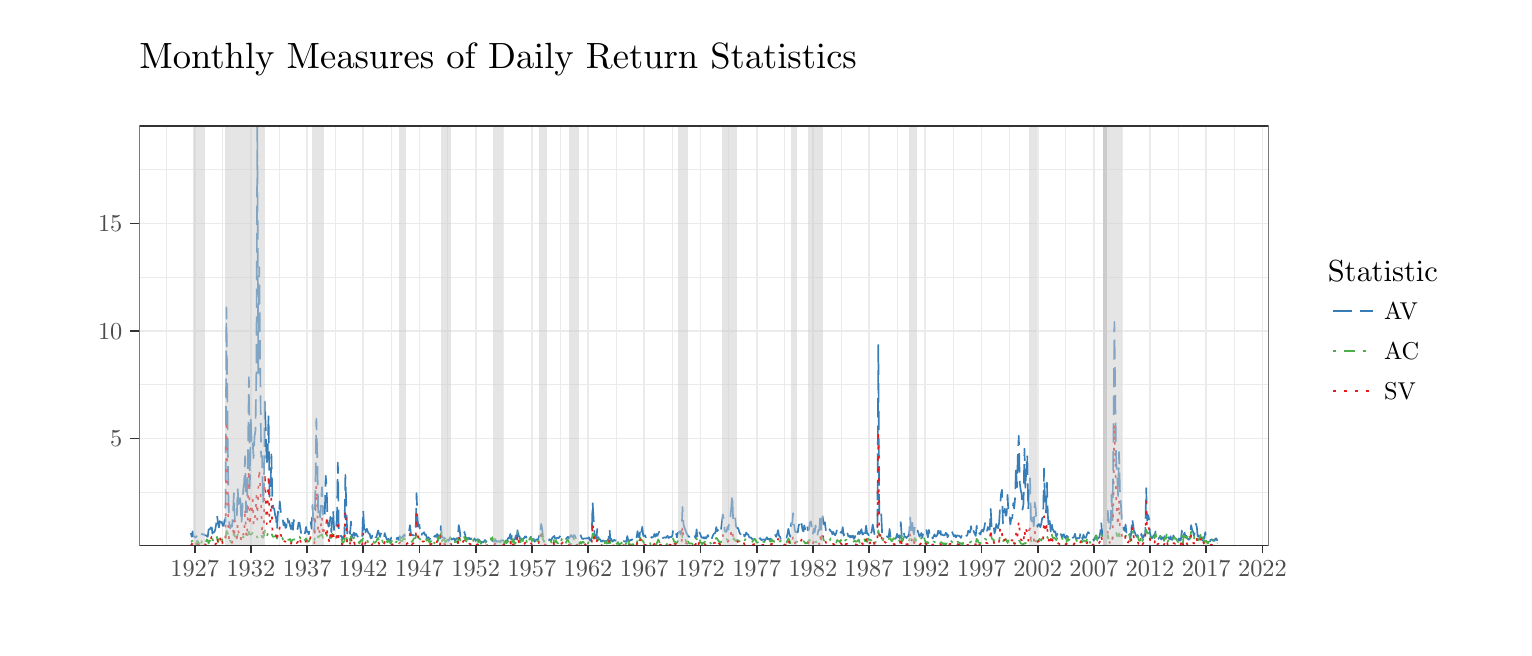
\begin{tikzpicture}[x=1.25pt,y=1pt]
\definecolor{fillColor}{RGB}{255,255,255}
\path[use as bounding box,fill=fillColor,fill opacity=0.00] (0,0) rectangle (426.79,216.81);
\begin{scope}
\path[clip] (  0.00,  0.00) rectangle (426.79,216.81);
\definecolor{drawColor}{RGB}{255,255,255}
\definecolor{fillColor}{RGB}{255,255,255}

\path[draw=drawColor,line width= 0.6pt,line join=round,line cap=round,fill=fillColor] (  0.00,  0.00) rectangle (426.79,216.81);
\end{scope}
\begin{scope}
\path[clip] ( 32.32, 29.59) rectangle (358.76,181.36);
\definecolor{fillColor}{RGB}{255,255,255}

\path[fill=fillColor] ( 32.32, 29.59) rectangle (358.76,181.36);
\definecolor{drawColor}{gray}{0.92}

\path[draw=drawColor,line width= 0.3pt,line join=round] ( 32.32, 48.97) --
	(358.76, 48.97);

\path[draw=drawColor,line width= 0.3pt,line join=round] ( 32.32, 87.81) --
	(358.76, 87.81);

\path[draw=drawColor,line width= 0.3pt,line join=round] ( 32.32,126.66) --
	(358.76,126.66);

\path[draw=drawColor,line width= 0.3pt,line join=round] ( 32.32,165.51) --
	(358.76,165.51);

\path[draw=drawColor,line width= 0.3pt,line join=round] ( 40.16, 29.59) --
	( 40.16,181.36);

\path[draw=drawColor,line width= 0.3pt,line join=round] ( 56.40, 29.59) --
	( 56.40,181.36);

\path[draw=drawColor,line width= 0.3pt,line join=round] ( 72.65, 29.59) --
	( 72.65,181.36);

\path[draw=drawColor,line width= 0.3pt,line join=round] ( 88.90, 29.59) --
	( 88.90,181.36);

\path[draw=drawColor,line width= 0.3pt,line join=round] (105.14, 29.59) --
	(105.14,181.36);

\path[draw=drawColor,line width= 0.3pt,line join=round] (121.39, 29.59) --
	(121.39,181.36);

\path[draw=drawColor,line width= 0.3pt,line join=round] (137.63, 29.59) --
	(137.63,181.36);

\path[draw=drawColor,line width= 0.3pt,line join=round] (153.88, 29.59) --
	(153.88,181.36);

\path[draw=drawColor,line width= 0.3pt,line join=round] (170.12, 29.59) --
	(170.12,181.36);

\path[draw=drawColor,line width= 0.3pt,line join=round] (186.37, 29.59) --
	(186.37,181.36);

\path[draw=drawColor,line width= 0.3pt,line join=round] (202.62, 29.59) --
	(202.62,181.36);

\path[draw=drawColor,line width= 0.3pt,line join=round] (218.86, 29.59) --
	(218.86,181.36);

\path[draw=drawColor,line width= 0.3pt,line join=round] (235.11, 29.59) --
	(235.11,181.36);

\path[draw=drawColor,line width= 0.3pt,line join=round] (251.35, 29.59) --
	(251.35,181.36);

\path[draw=drawColor,line width= 0.3pt,line join=round] (267.60, 29.59) --
	(267.60,181.36);

\path[draw=drawColor,line width= 0.3pt,line join=round] (283.85, 29.59) --
	(283.85,181.36);

\path[draw=drawColor,line width= 0.3pt,line join=round] (300.09, 29.59) --
	(300.09,181.36);

\path[draw=drawColor,line width= 0.3pt,line join=round] (316.33, 29.59) --
	(316.33,181.36);

\path[draw=drawColor,line width= 0.3pt,line join=round] (332.58, 29.59) --
	(332.58,181.36);

\path[draw=drawColor,line width= 0.3pt,line join=round] (348.83, 29.59) --
	(348.83,181.36);

\path[draw=drawColor,line width= 0.6pt,line join=round] ( 32.32, 68.39) --
	(358.76, 68.39);

\path[draw=drawColor,line width= 0.6pt,line join=round] ( 32.32,107.24) --
	(358.76,107.24);

\path[draw=drawColor,line width= 0.6pt,line join=round] ( 32.32,146.09) --
	(358.76,146.09);

\path[draw=drawColor,line width= 0.6pt,line join=round] ( 48.28, 29.59) --
	( 48.28,181.36);

\path[draw=drawColor,line width= 0.6pt,line join=round] ( 64.53, 29.59) --
	( 64.53,181.36);

\path[draw=drawColor,line width= 0.6pt,line join=round] ( 80.78, 29.59) --
	( 80.78,181.36);

\path[draw=drawColor,line width= 0.6pt,line join=round] ( 97.02, 29.59) --
	( 97.02,181.36);

\path[draw=drawColor,line width= 0.6pt,line join=round] (113.26, 29.59) --
	(113.26,181.36);

\path[draw=drawColor,line width= 0.6pt,line join=round] (129.51, 29.59) --
	(129.51,181.36);

\path[draw=drawColor,line width= 0.6pt,line join=round] (145.76, 29.59) --
	(145.76,181.36);

\path[draw=drawColor,line width= 0.6pt,line join=round] (162.00, 29.59) --
	(162.00,181.36);

\path[draw=drawColor,line width= 0.6pt,line join=round] (178.25, 29.59) --
	(178.25,181.36);

\path[draw=drawColor,line width= 0.6pt,line join=round] (194.49, 29.59) --
	(194.49,181.36);

\path[draw=drawColor,line width= 0.6pt,line join=round] (210.74, 29.59) --
	(210.74,181.36);

\path[draw=drawColor,line width= 0.6pt,line join=round] (226.99, 29.59) --
	(226.99,181.36);

\path[draw=drawColor,line width= 0.6pt,line join=round] (243.23, 29.59) --
	(243.23,181.36);

\path[draw=drawColor,line width= 0.6pt,line join=round] (259.47, 29.59) --
	(259.47,181.36);

\path[draw=drawColor,line width= 0.6pt,line join=round] (275.72, 29.59) --
	(275.72,181.36);

\path[draw=drawColor,line width= 0.6pt,line join=round] (291.97, 29.59) --
	(291.97,181.36);

\path[draw=drawColor,line width= 0.6pt,line join=round] (308.21, 29.59) --
	(308.21,181.36);

\path[draw=drawColor,line width= 0.6pt,line join=round] (324.45, 29.59) --
	(324.45,181.36);

\path[draw=drawColor,line width= 0.6pt,line join=round] (340.71, 29.59) --
	(340.71,181.36);

\path[draw=drawColor,line width= 0.6pt,line join=round] (356.95, 29.59) --
	(356.95,181.36);
\definecolor{drawColor}{RGB}{55,126,184}

\path[draw=drawColor,line width= 0.6pt,dash pattern=on 7pt off 3pt ,line join=round] ( 47.16, 34.17) --
	( 47.44, 32.84) --
	( 47.70, 34.78) --
	( 47.98, 32.86) --
	( 48.25, 32.94) --
	( 48.52, 32.62) --
	( 48.80, 32.80) --
	( 49.05, 33.83) --
	( 49.32, 33.16) --
	( 49.59, 33.11) --
	( 49.87, 33.40) --
	( 50.13, 33.08) --
	( 50.41, 33.91) --
	( 50.68, 33.68) --
	( 50.95, 33.69) --
	( 51.23, 33.38) --
	( 51.49, 33.36) --
	( 51.77, 33.07) --
	( 52.05, 32.83) --
	( 52.30, 35.46) --
	( 52.58, 35.55) --
	( 52.85, 35.87) --
	( 53.12, 37.94) --
	( 53.39, 33.99) --
	( 53.66, 34.55) --
	( 53.94, 34.49) --
	( 54.21, 35.34) --
	( 54.48, 37.37) --
	( 54.75, 40.62) --
	( 55.03, 37.58) --
	( 55.30, 36.21) --
	( 55.55, 38.54) --
	( 55.83, 36.42) --
	( 56.09, 38.23) --
	( 56.37, 36.86) --
	( 56.64, 36.77) --
	( 56.91, 38.91) --
	( 57.19, 38.25) --
	( 57.45,115.74) --
	( 57.73, 80.56) --
	( 58.00, 48.93) --
	( 58.27, 37.47) --
	( 58.55, 35.88) --
	( 58.80, 37.01) --
	( 59.07, 36.49) --
	( 59.34, 40.81) --
	( 59.62, 48.62) --
	( 59.88, 38.72) --
	( 60.16, 37.83) --
	( 60.43, 38.62) --
	( 60.70, 50.30) --
	( 60.98, 44.61) --
	( 61.24, 47.95) --
	( 61.52, 45.64) --
	( 61.79, 37.52) --
	( 62.04, 42.07) --
	( 62.32, 49.97) --
	( 62.59, 52.48) --
	( 62.86, 61.96) --
	( 63.13, 42.31) --
	( 63.40, 41.69) --
	( 63.68, 61.50) --
	( 63.95, 90.55) --
	( 64.22, 51.03) --
	( 64.49, 76.27) --
	( 64.77, 65.88) --
	( 65.04, 67.22) --
	( 65.30, 61.24) --
	( 65.58, 69.11) --
	( 65.84, 71.19) --
	( 66.12, 93.13) --
	( 66.38,181.36) --
	( 66.66, 91.93) --
	( 66.94,130.29) --
	( 67.20, 97.95) --
	( 67.48, 61.76) --
	( 67.75, 62.06) --
	( 68.02, 44.99) --
	( 68.30, 51.26) --
	( 68.55, 81.70) --
	( 68.82, 71.54) --
	( 69.09, 58.86) --
	( 69.36, 63.08) --
	( 69.63, 76.65) --
	( 69.91, 47.31) --
	( 70.18, 49.17) --
	( 70.45, 62.60) --
	( 70.73, 46.62) --
	( 70.99, 43.01) --
	( 71.27, 43.08) --
	( 71.54, 40.63) --
	( 71.79, 39.68) --
	( 72.07, 35.35) --
	( 72.34, 41.99) --
	( 72.61, 40.45) --
	( 72.88, 45.62) --
	( 73.15, 41.98) --
	( 73.43, 39.55) --
	( 73.70, 39.62) --
	( 73.97, 36.96) --
	( 74.24, 38.11) --
	( 74.52, 36.06) --
	( 74.79, 36.39) --
	( 75.04, 40.09) --
	( 75.32, 37.98) --
	( 75.58, 38.54) --
	( 75.86, 36.81) --
	( 76.13, 35.59) --
	( 76.40, 39.19) --
	( 76.68, 35.33) --
	( 76.94, 38.96) --
	( 77.22, 37.00) --
	( 77.49, 36.36) --
	( 77.76, 36.34) --
	( 78.04, 35.60) --
	( 78.30, 37.95) --
	( 78.57, 37.90) --
	( 78.84, 35.77) --
	( 79.11, 33.72) --
	( 79.38, 34.12) --
	( 79.66, 34.38) --
	( 79.93, 33.28) --
	( 80.20, 34.43) --
	( 80.48, 36.42) --
	( 80.74, 34.54) --
	( 81.02, 34.58) --
	( 81.29, 33.74) --
	( 81.54, 36.06) --
	( 81.82, 38.15) --
	( 82.09, 35.73) --
	( 82.36, 44.37) --
	( 82.63, 36.70) --
	( 82.90, 34.21) --
	( 83.18, 50.40) --
	( 83.45, 75.53) --
	( 83.72, 61.64) --
	( 83.99, 41.05) --
	( 84.27, 42.94) --
	( 84.54, 39.77) --
	( 84.79, 45.54) --
	( 85.07, 50.78) --
	( 85.33, 40.90) --
	( 85.61, 43.68) --
	( 85.88, 40.40) --
	( 86.15, 54.89) --
	( 86.43, 50.67) --
	( 86.69, 38.42) --
	( 86.97, 36.54) --
	( 87.24, 36.93) --
	( 87.51, 40.06) --
	( 87.79, 34.47) --
	( 88.04, 39.44) --
	( 88.31, 42.44) --
	( 88.58, 35.29) --
	( 88.86, 34.44) --
	( 89.12, 35.78) --
	( 89.40, 38.87) --
	( 89.67, 59.67) --
	( 89.94, 33.84) --
	( 90.22, 32.84) --
	( 90.48, 33.27) --
	( 90.76, 32.97) --
	( 91.03, 31.80) --
	( 91.29, 32.71) --
	( 91.57, 33.43) --
	( 91.84, 55.19) --
	( 92.11, 44.03) --
	( 92.38, 33.78) --
	( 92.65, 35.69) --
	( 92.93, 35.59) --
	( 93.20, 33.92) --
	( 93.47, 38.34) --
	( 93.74, 32.64) --
	( 94.01, 33.51) --
	( 94.29, 34.36) --
	( 94.54, 33.15) --
	( 94.82, 34.06) --
	( 95.08, 33.69) --
	( 95.36, 32.91) --
	( 95.62, 33.44) --
	( 95.90, 32.11) --
	( 96.18, 32.64) --
	( 96.44, 33.16) --
	( 96.72, 33.12) --
	( 96.99, 42.52) --
	( 97.26, 35.88) --
	( 97.54, 33.18) --
	( 97.79, 35.45) --
	( 98.06, 35.68) --
	( 98.33, 34.67) --
	( 98.60, 34.01) --
	( 98.87, 33.87) --
	( 99.15, 32.36) --
	( 99.42, 32.29) --
	( 99.69, 34.00) --
	( 99.97, 32.87) --
	(100.23, 33.42) --
	(100.51, 32.76) --
	(100.78, 32.61) --
	(101.03, 33.84) --
	(101.31, 35.10) --
	(101.58, 33.95) --
	(101.85, 32.80) --
	(102.12, 34.05) --
	(102.39, 33.37) --
	(102.67, 31.97) --
	(102.94, 32.14) --
	(103.21, 34.17) --
	(103.48, 33.07) --
	(103.76, 31.96) --
	(104.03, 31.70) --
	(104.29, 32.13) --
	(104.56, 31.59) --
	(104.83, 31.43) --
	(105.11, 32.52) --
	(105.37, 32.47) --
	(105.65, 31.90) --
	(105.93, 32.30) --
	(106.19, 31.40) --
	(106.47, 31.44) --
	(106.74, 32.42) --
	(107.01, 32.53) --
	(107.29, 31.66) --
	(107.54, 33.11) --
	(107.81, 32.38) --
	(108.08, 32.46) --
	(108.35, 32.83) --
	(108.62, 33.22) --
	(108.90, 33.69) --
	(109.17, 32.66) --
	(109.44, 32.97) --
	(109.72, 33.84) --
	(109.98, 34.16) --
	(110.26, 34.91) --
	(110.53, 37.01) --
	(110.78, 33.87) --
	(111.06, 33.30) --
	(111.33, 33.50) --
	(111.60, 33.30) --
	(111.87, 33.82) --
	(112.14, 33.83) --
	(112.42, 48.63) --
	(112.69, 39.21) --
	(112.96, 36.54) --
	(113.23, 37.24) --
	(113.50, 34.34) --
	(113.78, 32.99) --
	(114.03, 34.06) --
	(114.31, 34.01) --
	(114.57, 34.51) --
	(114.85, 33.50) --
	(115.11, 33.68) --
	(115.39, 32.30) --
	(115.67, 32.68) --
	(115.93, 32.59) --
	(116.21, 31.76) --
	(116.48, 33.17) --
	(116.75, 33.08) --
	(117.03, 33.09) --
	(117.29, 33.85) --
	(117.56, 32.85) --
	(117.83, 33.32) --
	(118.10, 32.78) --
	(118.37, 33.87) --
	(118.65, 32.26) --
	(118.92, 33.43) --
	(119.19, 32.18) --
	(119.46, 36.76) --
	(119.73, 32.80) --
	(120.01, 32.60) --
	(120.28, 32.50) --
	(120.53, 32.46) --
	(120.81, 31.64) --
	(121.07, 31.81) --
	(121.35, 32.98) --
	(121.62, 31.33) --
	(121.89, 32.00) --
	(122.17, 32.71) --
	(122.44, 31.79) --
	(122.71, 31.90) --
	(122.98, 32.15) --
	(123.25, 32.29) --
	(123.53, 31.34) --
	(123.78, 32.00) --
	(124.05, 32.33) --
	(124.32, 31.76) --
	(124.60, 37.07) --
	(124.86, 35.58) --
	(125.14, 32.36) --
	(125.42, 32.19) --
	(125.68, 32.92) --
	(125.96, 33.92) --
	(126.23, 34.58) --
	(126.50, 33.39) --
	(126.78, 31.72) --
	(127.03, 32.46) --
	(127.30, 31.91) --
	(127.57, 32.48) --
	(127.84, 31.98) --
	(128.11, 32.28) --
	(128.39, 31.81) --
	(128.66, 31.50) --
	(128.93, 33.24) --
	(129.21, 32.00) --
	(129.47, 31.33) --
	(129.75, 31.73) --
	(130.02, 31.81) --
	(130.28, 31.92) --
	(130.56, 31.66) --
	(130.82, 31.23) --
	(131.10, 30.85) --
	(131.37, 30.98) --
	(131.64, 30.73) --
	(131.92, 31.13) --
	(132.19, 31.68) --
	(132.46, 31.19) --
	(132.73, 31.13) --
	(133.00, 31.01) --
	(133.28, 30.91) --
	(133.53, 31.55) --
	(133.80, 31.94) --
	(134.07, 31.04) --
	(134.35, 31.91) --
	(134.61, 31.07) --
	(134.89, 31.12) --
	(135.17, 32.00) --
	(135.43, 31.23) --
	(135.71, 31.03) --
	(135.97, 31.28) --
	(136.25, 31.20) --
	(136.53, 31.09) --
	(136.78, 31.42) --
	(137.05, 31.61) --
	(137.32, 31.37) --
	(137.59, 32.58) --
	(137.86, 31.80) --
	(138.14, 32.32) --
	(138.41, 31.45) --
	(138.68, 31.61) --
	(138.95, 32.52) --
	(139.22, 32.35) --
	(139.50, 33.83) --
	(139.77, 31.86) --
	(140.02, 33.92) --
	(140.30, 31.71) --
	(140.56, 31.92) --
	(140.84, 31.90) --
	(141.11, 33.31) --
	(141.38, 31.88) --
	(141.66, 36.40) --
	(141.93, 32.99) --
	(142.20, 32.93) --
	(142.47, 31.38) --
	(142.74, 31.99) --
	(143.02, 31.81) --
	(143.28, 32.11) --
	(143.55, 32.46) --
	(143.82, 33.02) --
	(144.10, 32.87) --
	(144.36, 31.69) --
	(144.64, 32.09) --
	(144.91, 31.58) --
	(145.18, 32.52) --
	(145.46, 32.83) --
	(145.72, 31.89) --
	(146.00, 31.71) --
	(146.28, 32.08) --
	(146.53, 31.03) --
	(146.80, 31.48) --
	(147.07, 31.88) --
	(147.34, 31.89) --
	(147.61, 31.93) --
	(147.89, 33.30) --
	(148.16, 32.54) --
	(148.43, 37.47) --
	(148.70, 35.86) --
	(148.97, 32.73) --
	(149.25, 32.47) --
	(149.52, 31.61) --
	(149.77, 31.51) --
	(150.05, 31.75) --
	(150.31, 31.34) --
	(150.59, 31.34) --
	(150.86, 31.96) --
	(151.13, 31.57) --
	(151.41, 31.65) --
	(151.68, 32.56) --
	(151.95, 32.81) --
	(152.22, 33.13) --
	(152.49, 32.25) --
	(152.77, 32.09) --
	(153.02, 32.46) --
	(153.29, 32.51) --
	(153.56, 32.37) --
	(153.84, 33.02) --
	(154.10, 32.62) --
	(154.38, 32.43) --
	(154.66, 33.30) --
	(154.92, 32.60) --
	(155.20, 32.43) --
	(155.47, 32.22) --
	(155.74, 32.08) --
	(156.02, 32.72) --
	(156.27, 32.80) --
	(156.55, 32.26) --
	(156.82, 32.99) --
	(157.09, 33.48) --
	(157.36, 32.81) --
	(157.64, 32.64) --
	(157.91, 33.46) --
	(158.18, 33.17) --
	(158.45, 32.32) --
	(158.72, 32.71) --
	(159.00, 32.88) --
	(159.27, 32.31) --
	(159.52, 32.87) --
	(159.80, 33.65) --
	(160.06, 32.65) --
	(160.34, 32.11) --
	(160.61, 32.04) --
	(160.88, 32.28) --
	(161.16, 32.27) --
	(161.43, 32.21) --
	(161.70, 32.38) --
	(161.97, 32.21) --
	(162.24, 32.65) --
	(162.52, 31.54) --
	(162.77, 31.48) --
	(163.04, 32.40) --
	(163.31, 45.35) --
	(163.59, 39.25) --
	(163.85, 33.87) --
	(164.13, 32.42) --
	(164.41, 32.16) --
	(164.67, 35.91) --
	(164.95, 32.74) --
	(165.21, 31.93) --
	(165.49, 31.97) --
	(165.77, 31.14) --
	(166.02, 31.10) --
	(166.29, 31.55) --
	(166.56, 31.37) --
	(166.83, 31.12) --
	(167.10, 31.41) --
	(167.38, 31.29) --
	(167.65, 31.46) --
	(167.92, 32.27) --
	(168.19, 35.72) --
	(168.46, 31.64) --
	(168.74, 32.03) --
	(169.01, 31.08) --
	(169.27, 31.30) --
	(169.55, 31.74) --
	(169.81, 31.42) --
	(170.09, 31.54) --
	(170.36, 31.25) --
	(170.63, 31.26) --
	(170.91, 31.21) --
	(171.17, 31.14) --
	(171.45, 31.24) --
	(171.72, 31.53) --
	(171.99, 31.11) --
	(172.27, 31.29) --
	(172.52, 31.16) --
	(172.79, 31.10) --
	(173.06, 31.23) --
	(173.34, 33.10) --
	(173.60, 31.54) --
	(173.88, 31.16) --
	(174.15, 31.69) --
	(174.42, 31.61) --
	(174.70, 31.78) --
	(174.96, 32.55) --
	(175.24, 32.09) --
	(175.52, 32.13) --
	(175.76, 33.28) --
	(176.04, 32.64) --
	(176.31, 34.89) --
	(176.58, 32.82) --
	(176.85, 32.61) --
	(177.13, 36.14) --
	(177.40, 34.65) --
	(177.67, 36.43) --
	(177.94, 33.17) --
	(178.21, 33.13) --
	(178.49, 33.40) --
	(178.76, 32.31) --
	(179.01, 33.02) --
	(179.29, 32.82) --
	(179.55, 33.02) --
	(179.83, 33.50) --
	(180.10, 33.05) --
	(180.37, 32.46) --
	(180.65, 32.62) --
	(180.92, 32.93) --
	(181.19, 33.85) --
	(181.46, 32.87) --
	(181.73, 33.83) --
	(182.01, 33.17) --
	(182.27, 33.91) --
	(182.54, 34.64) --
	(182.81, 33.17) --
	(183.09, 33.45) --
	(183.35, 33.50) --
	(183.63, 32.37) --
	(183.90, 32.57) --
	(184.17, 32.66) --
	(184.45, 32.40) --
	(184.71, 32.82) --
	(184.99, 33.20) --
	(185.27, 32.39) --
	(185.51, 32.67) --
	(185.79, 32.82) --
	(186.06, 32.72) --
	(186.33, 33.14) --
	(186.60, 35.29) --
	(186.88, 33.65) --
	(187.15, 33.61) --
	(187.42, 34.22) --
	(187.69, 32.64) --
	(187.96, 34.25) --
	(188.24, 34.46) --
	(188.51, 34.83) --
	(188.76, 33.66) --
	(189.04, 34.55) --
	(189.30, 43.59) --
	(189.58, 37.20) --
	(189.85, 36.24) --
	(190.12, 35.28) --
	(190.40, 34.34) --
	(190.66, 33.73) --
	(190.94, 32.99) --
	(191.21, 32.80) --
	(191.48, 33.01) --
	(191.76, 32.56) --
	(192.01, 32.64) --
	(192.28, 32.86) --
	(192.55, 32.18) --
	(192.83, 33.09) --
	(193.09, 32.28) --
	(193.37, 35.53) --
	(193.64, 32.04) --
	(193.91, 32.67) --
	(194.19, 34.40) --
	(194.45, 33.77) --
	(194.73, 32.67) --
	(195.01, 32.42) --
	(195.26, 32.69) --
	(195.54, 32.18) --
	(195.81, 32.72) --
	(196.08, 32.22) --
	(196.35, 32.81) --
	(196.62, 33.47) --
	(196.90, 32.11) --
	(197.17, 32.98) --
	(197.44, 32.87) --
	(197.71, 31.96) --
	(197.99, 33.00) --
	(198.26, 33.77) --
	(198.51, 34.10) --
	(198.79, 34.22) --
	(199.05, 36.34) --
	(199.33, 34.88) --
	(199.60, 35.27) --
	(199.87, 33.85) --
	(200.15, 34.40) --
	(200.41, 35.27) --
	(200.69, 38.10) --
	(200.96, 40.90) --
	(201.23, 39.24) --
	(201.51, 34.92) --
	(201.76, 34.66) --
	(202.03, 34.67) --
	(202.30, 36.41) --
	(202.58, 35.44) --
	(202.84, 39.91) --
	(203.12, 39.87) --
	(203.39, 43.17) --
	(203.66, 48.13) --
	(203.94, 38.73) --
	(204.20, 38.52) --
	(204.48, 40.15) --
	(204.76, 36.61) --
	(205.00, 35.99) --
	(205.28, 36.11) --
	(205.55, 35.27) --
	(205.82, 34.21) --
	(206.09, 33.74) --
	(206.37, 34.95) --
	(206.64, 35.09) --
	(206.91, 34.99) --
	(207.18, 32.90) --
	(207.45, 33.39) --
	(207.73, 34.38) --
	(208.00, 33.65) --
	(208.26, 33.77) --
	(208.54, 32.82) --
	(208.80, 32.50) --
	(209.08, 32.66) --
	(209.35, 31.99) --
	(209.62, 32.13) --
	(209.90, 32.11) --
	(210.16, 32.64) --
	(210.44, 32.72) --
	(210.71, 32.29) --
	(210.98, 32.19) --
	(211.26, 31.64) --
	(211.51, 32.05) --
	(211.78, 32.35) --
	(212.05, 31.68) --
	(212.33, 31.71) --
	(212.59, 31.90) --
	(212.87, 31.92) --
	(213.14, 31.46) --
	(213.41, 32.04) --
	(213.69, 32.68) --
	(213.95, 31.96) --
	(214.23, 32.13) --
	(214.50, 31.63) --
	(214.75, 32.19) --
	(215.03, 33.04) --
	(215.30, 33.01) --
	(215.57, 32.60) --
	(215.84, 32.38) --
	(216.11, 33.51) --
	(216.39, 32.80) --
	(216.66, 33.94) --
	(216.93, 35.22) --
	(217.20, 33.19) --
	(217.48, 32.84) --
	(217.75, 31.85) --
	(218.00, 32.45) --
	(218.28, 32.10) --
	(218.54, 32.84) --
	(218.82, 32.64) --
	(219.09, 32.65) --
	(219.36, 32.52) --
	(219.64, 33.79) --
	(219.90, 35.73) --
	(220.18, 34.00) --
	(220.45, 32.85) --
	(220.72, 37.82) --
	(221.00, 37.30) --
	(221.26, 41.37) --
	(221.53, 37.28) --
	(221.80, 34.96) --
	(222.07, 34.40) --
	(222.34, 34.58) --
	(222.62, 34.45) --
	(222.89, 37.09) --
	(223.16, 37.21) --
	(223.44, 36.02) --
	(223.70, 37.77) --
	(223.98, 35.33) --
	(224.25, 34.77) --
	(224.50, 36.97) --
	(224.78, 35.57) --
	(225.05, 34.96) --
	(225.32, 37.00) --
	(225.59, 35.17) --
	(225.86, 35.48) --
	(226.14, 38.08) --
	(226.41, 38.37) --
	(226.68, 36.53) --
	(226.95, 33.53) --
	(227.23, 35.74) --
	(227.50, 34.44) --
	(227.75, 36.98) --
	(228.03, 34.39) --
	(228.29, 33.16) --
	(228.57, 35.32) --
	(228.84, 35.10) --
	(229.11, 40.38) --
	(229.39, 35.40) --
	(229.65, 41.58) --
	(229.93, 38.95) --
	(230.20, 37.35) --
	(230.47, 38.05) --
	(230.75, 35.01) --
	(231.00, 35.53) --
	(231.27, 34.42) --
	(231.54, 34.36) --
	(231.82, 35.58) --
	(232.08, 34.86) --
	(232.36, 34.81) --
	(232.63, 33.77) --
	(232.90, 34.59) --
	(233.18, 33.73) --
	(233.44, 33.37) --
	(233.72, 34.20) --
	(234.00, 35.67) --
	(234.25, 34.58) --
	(234.53, 33.78) --
	(234.80, 33.82) --
	(235.07, 34.58) --
	(235.34, 34.21) --
	(235.61, 36.27) --
	(235.89, 33.22) --
	(236.16, 34.05) --
	(236.43, 32.67) --
	(236.70, 33.31) --
	(236.98, 34.06) --
	(237.25, 32.96) --
	(237.50, 33.24) --
	(237.78, 32.59) --
	(238.04, 33.21) --
	(238.32, 32.65) --
	(238.59, 33.23) --
	(238.86, 32.06) --
	(239.14, 32.64) --
	(239.40, 33.89) --
	(239.68, 32.57) --
	(239.95, 33.89) --
	(240.22, 34.72) --
	(240.50, 33.85) --
	(240.75, 34.48) --
	(241.02, 35.61) --
	(241.29, 33.69) --
	(241.57, 33.71) --
	(241.83, 35.83) --
	(242.11, 34.13) --
	(242.38, 36.87) --
	(242.65, 33.96) --
	(242.93, 33.94) --
	(243.19, 33.18) --
	(243.47, 35.03) --
	(243.74, 34.07) --
	(243.99, 34.68) --
	(244.27, 37.27) --
	(244.54, 35.70) --
	(244.81, 33.49) --
	(245.08, 33.54) --
	(245.35, 34.28) --
	(245.63, 35.16) --
	(245.90,102.16) --
	(246.17, 40.57) --
	(246.44, 40.65) --
	(246.72, 41.83) --
	(246.99, 34.40) --
	(247.25, 34.88) --
	(247.53, 34.96) --
	(247.79, 33.85) --
	(248.07, 33.92) --
	(248.33, 33.07) --
	(248.61, 32.73) --
	(248.89, 32.61) --
	(249.15, 35.65) --
	(249.43, 32.62) --
	(249.70, 31.93) --
	(249.97, 32.53) --
	(250.25, 32.33) --
	(250.50, 32.77) --
	(250.77, 32.06) --
	(251.04, 32.49) --
	(251.31, 33.89) --
	(251.58, 32.72) --
	(251.86, 33.37) --
	(252.13, 32.10) --
	(252.40, 38.16) --
	(252.68, 32.73) --
	(252.94, 32.93) --
	(253.22, 34.80) --
	(253.49, 32.84) --
	(253.74, 32.85) --
	(254.02, 32.40) --
	(254.29, 32.82) --
	(254.56, 33.06) --
	(254.83, 33.99) --
	(255.10, 39.80) --
	(255.38, 35.17) --
	(255.65, 39.30) --
	(255.92, 35.29) --
	(256.19, 33.74) --
	(256.47, 36.67) --
	(256.74, 35.91) --
	(256.99, 34.64) --
	(257.27, 35.10) --
	(257.53, 34.08) --
	(257.81, 32.86) --
	(258.08, 33.41) --
	(258.35, 34.20) --
	(258.63, 32.57) --
	(258.89, 34.22) --
	(259.17, 34.22) --
	(259.44, 35.01) --
	(259.71, 35.97) --
	(259.99, 33.95) --
	(260.25, 32.64) --
	(260.52, 35.35) --
	(260.79, 33.04) --
	(261.06, 33.79) --
	(261.33, 33.53) --
	(261.61, 32.22) --
	(261.88, 33.06) --
	(262.15, 33.73) --
	(262.43, 32.91) --
	(262.69, 33.01) --
	(262.97, 33.67) --
	(263.24, 35.06) --
	(263.49, 33.99) --
	(263.77, 36.19) --
	(264.04, 33.51) --
	(264.31, 33.76) --
	(264.58, 33.39) --
	(264.85, 33.38) --
	(265.13, 33.39) --
	(265.40, 34.28) --
	(265.67, 34.06) --
	(265.94, 32.68) --
	(266.21, 33.47) --
	(266.49, 33.30) --
	(266.74, 34.10) --
	(267.02, 35.29) --
	(267.28, 34.45) --
	(267.56, 33.58) --
	(267.82, 32.96) --
	(268.10, 33.47) --
	(268.38, 32.62) --
	(268.64, 33.32) --
	(268.92, 33.27) --
	(269.19, 33.19) --
	(269.46, 33.01) --
	(269.74, 32.43) --
	(269.99, 33.14) --
	(270.26, 33.13) --
	(270.53, 33.80) --
	(270.80, 33.72) --
	(271.07, 34.40) --
	(271.35, 33.14) --
	(271.62, 33.36) --
	(271.89, 35.06) --
	(272.17, 34.39) --
	(272.43, 34.54) --
	(272.71, 36.68) --
	(272.98, 34.29) --
	(273.24, 35.65) --
	(273.52, 34.65) --
	(273.78, 33.89) --
	(274.06, 33.17) --
	(274.33, 36.84) --
	(274.60, 33.86) --
	(274.88, 33.32) --
	(275.15, 34.20) --
	(275.42, 33.63) --
	(275.69, 35.01) --
	(275.96, 35.41) --
	(276.24, 34.73) --
	(276.49, 35.90) --
	(276.76, 37.81) --
	(277.03, 35.05) --
	(277.31, 34.98) --
	(277.57, 36.41) --
	(277.85, 35.39) --
	(278.13, 35.55) --
	(278.39, 42.94) --
	(278.67, 35.84) --
	(278.94, 36.91) --
	(279.21, 37.10) --
	(279.49, 34.06) --
	(279.74, 35.08) --
	(280.01, 37.46) --
	(280.28, 34.42) --
	(280.55, 36.40) --
	(280.82, 37.75) --
	(281.10, 43.62) --
	(281.37, 48.19) --
	(281.64, 49.81) --
	(281.92, 37.70) --
	(282.18, 40.49) --
	(282.46, 43.00) --
	(282.73, 40.46) --
	(282.98, 40.74) --
	(283.26, 47.99) --
	(283.53, 40.91) --
	(283.80, 40.77) --
	(284.07, 37.32) --
	(284.34, 39.61) --
	(284.62, 39.51) --
	(284.89, 44.97) --
	(285.16, 43.00) --
	(285.43, 46.65) --
	(285.70, 57.88) --
	(285.98, 50.72) --
	(286.24, 62.42) --
	(286.51, 69.37) --
	(286.78, 52.36) --
	(287.06, 49.90) --
	(287.32, 48.27) --
	(287.60, 42.61) --
	(287.88, 44.88) --
	(288.14, 64.69) --
	(288.42, 50.20) --
	(288.68, 57.47) --
	(288.96, 62.62) --
	(289.24, 42.54) --
	(289.49, 51.48) --
	(289.76, 54.03) --
	(290.03, 39.25) --
	(290.30, 38.04) --
	(290.57, 40.40) --
	(290.85, 36.66) --
	(291.12, 45.21) --
	(291.39, 43.15) --
	(291.66, 37.22) --
	(291.93, 36.42) --
	(292.21, 37.43) --
	(292.48, 37.29) --
	(292.73, 36.31) --
	(293.01, 37.50) --
	(293.27, 39.58) --
	(293.55, 39.74) --
	(293.82, 57.57) --
	(294.09, 44.48) --
	(294.37, 41.58) --
	(294.64, 52.42) --
	(294.91, 40.60) --
	(295.18, 35.62) --
	(295.45, 38.58) --
	(295.73, 34.72) --
	(295.98, 38.35) --
	(296.25, 35.73) --
	(296.52, 35.03) --
	(296.80, 34.47) --
	(297.06, 34.82) --
	(297.34, 32.78) --
	(297.62, 33.80) --
	(297.88, 33.93) --
	(298.16, 32.57) --
	(298.43, 32.41) --
	(298.70, 33.85) --
	(298.98, 32.46) --
	(299.24, 33.50) --
	(299.51, 33.75) --
	(299.78, 32.75) --
	(300.05, 32.18) --
	(300.32, 33.22) --
	(300.60, 32.94) --
	(300.87, 32.55) --
	(301.14, 33.68) --
	(301.41, 32.59) --
	(301.68, 32.41) --
	(301.96, 32.54) --
	(302.23, 32.50) --
	(302.48, 32.88) --
	(302.76, 33.93) --
	(303.02, 32.22) --
	(303.30, 32.05) --
	(303.57, 32.44) --
	(303.84, 32.27) --
	(304.12, 32.52) --
	(304.39, 34.81) --
	(304.66, 32.85) --
	(304.93, 31.94) --
	(305.20, 33.60) --
	(305.48, 32.56) --
	(305.73, 32.45) --
	(306.00, 32.79) --
	(306.27, 33.92) --
	(306.55, 34.52) --
	(306.81, 34.18) --
	(307.09, 32.70) --
	(307.37, 32.59) --
	(307.63, 32.88) --
	(307.91, 32.46) --
	(308.18, 31.42) --
	(308.45, 32.58) --
	(308.73, 32.57) --
	(308.98, 32.66) --
	(309.25, 32.10) --
	(309.52, 32.39) --
	(309.79, 32.61) --
	(310.06, 34.39) --
	(310.34, 38.23) --
	(310.61, 33.14) --
	(310.88, 35.40) --
	(311.16, 40.41) --
	(311.42, 34.77) --
	(311.70, 41.17) --
	(311.97, 37.52) --
	(312.23, 42.23) --
	(312.51, 37.93) --
	(312.77, 35.19) --
	(313.05, 36.78) --
	(313.32, 48.10) --
	(313.59, 38.77) --
	(313.87, 67.97) --
	(314.14,110.47) --
	(314.41, 81.00) --
	(314.68, 59.45) --
	(314.95, 54.78) --
	(315.23, 47.51) --
	(315.48, 63.47) --
	(315.75, 49.10) --
	(316.02, 44.73) --
	(316.30, 37.89) --
	(316.56, 37.89) --
	(316.84, 35.54) --
	(317.12, 34.97) --
	(317.38, 37.27) --
	(317.66, 33.86) --
	(317.92, 32.95) --
	(318.20, 34.20) --
	(318.48, 33.94) --
	(318.73, 32.12) --
	(319.00, 34.03) --
	(319.27, 39.49) --
	(319.54, 37.27) --
	(319.81, 34.97) --
	(320.09, 34.35) --
	(320.36, 33.22) --
	(320.63, 33.08) --
	(320.90, 33.48) --
	(321.17, 31.95) --
	(321.45, 33.06) --
	(321.72, 32.98) --
	(321.97, 33.95) --
	(322.25, 32.36) --
	(322.51, 32.56) --
	(322.79, 33.63) --
	(323.06, 33.57) --
	(323.33, 50.46) --
	(323.61, 38.59) --
	(323.88, 40.71) --
	(324.15, 39.30) --
	(324.42, 34.19) --
	(324.69, 33.00) --
	(324.97, 32.27) --
	(325.23, 32.56) --
	(325.50, 33.48) --
	(325.77, 33.39) --
	(326.05, 34.74) --
	(326.31, 33.81) --
	(326.59, 31.97) --
	(326.86, 32.06) --
	(327.13, 32.58) --
	(327.41, 33.15) --
	(327.67, 31.85) --
	(327.95, 32.67) --
	(328.23, 32.32) --
	(328.47, 31.42) --
	(328.75, 33.96) --
	(329.02, 32.67) --
	(329.29, 33.15) --
	(329.56, 32.88) --
	(329.84, 32.33) --
	(330.11, 31.90) --
	(330.38, 33.04) --
	(330.65, 31.83) --
	(330.92, 31.72) --
	(331.20, 33.33) --
	(331.47, 32.47) --
	(331.72, 32.05) --
	(332.00, 33.25) --
	(332.26, 31.61) --
	(332.54, 31.35) --
	(332.81, 32.28) --
	(333.08, 31.42) --
	(333.36, 31.66) --
	(333.63, 35.09) --
	(333.90, 31.88) --
	(334.17, 33.64) --
	(334.44, 34.33) --
	(334.72, 32.47) --
	(334.97, 33.18) --
	(335.24, 32.39) --
	(335.51, 31.87) --
	(335.79, 31.85) --
	(336.05, 33.59) --
	(336.33, 37.03) --
	(336.61, 35.31) --
	(336.87, 34.76) --
	(337.15, 33.12) --
	(337.41, 34.53) --
	(337.69, 37.59) --
	(337.97, 36.50) --
	(338.22, 32.98) --
	(338.50, 33.27) --
	(338.77, 32.53) --
	(339.04, 34.56) --
	(339.31, 31.92) --
	(339.59, 31.52) --
	(339.86, 32.71) --
	(340.13, 32.14) --
	(340.40, 34.53) --
	(340.67, 31.74) --
	(340.95, 31.83) --
	(341.22, 31.47) --
	(341.47, 31.45) --
	(341.75, 31.14) --
	(342.01, 31.80) --
	(342.29, 31.92) --
	(342.56, 31.61) --
	(342.83, 31.73) --
	(343.11, 31.36) --
	(343.37, 32.20) --
	(343.65, 32.21) --
	(343.92, 31.36);
\definecolor{drawColor}{RGB}{77,175,74}

\path[draw=drawColor,line width= 0.6pt,dash pattern=on 1pt off 3pt on 4pt off 3pt ,line join=round] ( 47.16, 31.09) --
	( 47.44, 31.04) --
	( 47.70, 32.13) --
	( 47.98, 30.61) --
	( 48.25, 30.76) --
	( 48.52, 30.91) --
	( 48.80, 30.05) --
	( 49.05, 31.45) --
	( 49.32, 30.96) --
	( 49.59, 30.23) --
	( 49.87, 31.57) --
	( 50.13, 30.02) --
	( 50.41, 31.73) --
	( 50.68, 31.32) --
	( 50.95, 31.87) --
	( 51.23, 30.91) --
	( 51.49, 30.82) --
	( 51.77, 31.87) --
	( 52.05, 31.63) --
	( 52.30, 30.43) --
	( 52.58, 31.28) --
	( 52.85, 31.65) --
	( 53.12, 33.41) --
	( 53.39, 32.34) --
	( 53.66, 31.09) --
	( 53.94, 30.76) --
	( 54.21, 30.65) --
	( 54.48, 30.57) --
	( 54.75, 32.83) --
	( 55.03, 30.87) --
	( 55.30, 32.73) --
	( 55.55, 32.98) --
	( 55.83, 31.97) --
	( 56.09, 32.51) --
	( 56.37, 30.65) --
	( 56.64, 30.58) --
	( 56.91, 31.77) --
	( 57.19, 31.88) --
	( 57.45, 34.93) --
	( 57.73, 34.55) --
	( 58.00, 33.29) --
	( 58.27, 30.99) --
	( 58.55, 31.46) --
	( 58.80, 30.65) --
	( 59.07, 31.33) --
	( 59.34, 32.63) --
	( 59.62, 34.08) --
	( 59.88, 32.95) --
	( 60.16, 32.90) --
	( 60.43, 32.58) --
	( 60.70, 33.65) --
	( 60.98, 33.11) --
	( 61.24, 33.31) --
	( 61.52, 33.06) --
	( 61.79, 32.01) --
	( 62.04, 32.40) --
	( 62.32, 32.87) --
	( 62.59, 32.43) --
	( 62.86, 33.90) --
	( 63.13, 33.52) --
	( 63.40, 32.96) --
	( 63.68, 33.77) --
	( 63.95, 34.65) --
	( 64.22, 33.71) --
	( 64.49, 33.64) --
	( 64.77, 33.83) --
	( 65.04, 34.30) --
	( 65.30, 33.26) --
	( 65.58, 32.72) --
	( 65.84, 33.18) --
	( 66.12, 33.54) --
	( 66.38, 32.57) --
	( 66.66, 33.63) --
	( 66.94, 34.37) --
	( 67.20, 34.35) --
	( 67.48, 34.07) --
	( 67.75, 32.77) --
	( 68.02, 32.49) --
	( 68.30, 33.24) --
	( 68.55, 35.17) --
	( 68.82, 33.69) --
	( 69.09, 32.71) --
	( 69.36, 33.83) --
	( 69.63, 34.58) --
	( 69.91, 34.20) --
	( 70.18, 33.61) --
	( 70.45, 34.37) --
	( 70.73, 33.17) --
	( 70.99, 32.79) --
	( 71.27, 32.95) --
	( 71.54, 33.00) --
	( 71.79, 33.37) --
	( 72.07, 32.21) --
	( 72.34, 33.09) --
	( 72.61, 33.35) --
	( 72.88, 33.71) --
	( 73.15, 33.16) --
	( 73.43, 32.83) --
	( 73.70, 32.25) --
	( 73.97, 31.15) --
	( 74.24, 32.08) --
	( 74.52, 31.93) --
	( 74.79, 32.28) --
	( 75.04, 32.02) --
	( 75.32, 31.75) --
	( 75.58, 31.73) --
	( 75.86, 32.07) --
	( 76.13, 31.00) --
	( 76.40, 31.46) --
	( 76.68, 31.77) --
	( 76.94, 31.86) --
	( 77.22, 31.85) --
	( 77.49, 31.80) --
	( 77.76, 31.15) --
	( 78.04, 31.42) --
	( 78.30, 32.64) --
	( 78.57, 32.89) --
	( 78.84, 32.31) --
	( 79.11, 31.29) --
	( 79.38, 30.92) --
	( 79.66, 31.97) --
	( 79.93, 31.55) --
	( 80.20, 31.77) --
	( 80.48, 32.24) --
	( 80.74, 31.67) --
	( 81.02, 31.06) --
	( 81.29, 31.10) --
	( 81.54, 31.78) --
	( 81.82, 33.27) --
	( 82.09, 32.57) --
	( 82.36, 32.47) --
	( 82.63, 31.80) --
	( 82.90, 31.69) --
	( 83.18, 33.87) --
	( 83.45, 34.07) --
	( 83.72, 34.08) --
	( 83.99, 32.57) --
	( 84.27, 33.07) --
	( 84.54, 33.24) --
	( 84.79, 33.45) --
	( 85.07, 33.76) --
	( 85.33, 32.44) --
	( 85.61, 33.21) --
	( 85.88, 32.88) --
	( 86.15, 32.93) --
	( 86.43, 34.14) --
	( 86.69, 31.94) --
	( 86.97, 32.79) --
	( 87.24, 31.92) --
	( 87.51, 33.47) --
	( 87.79, 32.47) --
	( 88.04, 33.91) --
	( 88.31, 33.40) --
	( 88.58, 32.23) --
	( 88.86, 32.67) --
	( 89.12, 32.34) --
	( 89.40, 33.27) --
	( 89.67, 32.48) --
	( 89.94, 31.87) --
	( 90.22, 31.32) --
	( 90.48, 31.11) --
	( 90.76, 31.97) --
	( 91.03, 30.47) --
	( 91.29, 30.92) --
	( 91.57, 31.26) --
	( 91.84, 33.94) --
	( 92.11, 33.30) --
	( 92.38, 30.97) --
	( 92.65, 32.57) --
	( 92.93, 32.60) --
	( 93.20, 31.32) --
	( 93.47, 33.07) --
	( 93.74, 30.53) --
	( 94.01, 31.53) --
	( 94.29, 32.65) --
	( 94.54, 31.27) --
	( 94.82, 31.55) --
	( 95.08, 30.92) --
	( 95.36, 31.23) --
	( 95.62, 31.04) --
	( 95.90, 30.40) --
	( 96.18, 31.34) --
	( 96.44, 31.67) --
	( 96.72, 31.27) --
	( 96.99, 32.59) --
	( 97.26, 31.46) --
	( 97.54, 31.47) --
	( 97.79, 31.96) --
	( 98.06, 32.00) --
	( 98.33, 30.93) --
	( 98.60, 31.30) --
	( 98.87, 31.66) --
	( 99.15, 30.67) --
	( 99.42, 30.57) --
	( 99.69, 31.25) --
	( 99.97, 31.06) --
	(100.23, 30.59) --
	(100.51, 30.80) --
	(100.78, 31.22) --
	(101.03, 31.87) --
	(101.31, 32.45) --
	(101.58, 31.30) --
	(101.85, 31.57) --
	(102.12, 32.70) --
	(102.39, 31.97) --
	(102.67, 30.86) --
	(102.94, 31.39) --
	(103.21, 32.44) --
	(103.48, 31.26) --
	(103.76, 31.14) --
	(104.03, 30.88) --
	(104.29, 31.23) --
	(104.56, 31.55) --
	(104.83, 30.47) --
	(105.11, 30.82) --
	(105.37, 31.60) --
	(105.65, 31.07) --
	(105.93, 32.16) --
	(106.19, 31.27) --
	(106.47, 30.87) --
	(106.74, 31.15) --
	(107.01, 31.26) --
	(107.29, 30.78) --
	(107.54, 32.78) --
	(107.81, 31.37) --
	(108.08, 31.26) --
	(108.35, 31.36) --
	(108.62, 32.41) --
	(108.90, 32.22) --
	(109.17, 31.69) --
	(109.44, 31.28) --
	(109.72, 31.69) --
	(109.98, 31.84) --
	(110.26, 32.24) --
	(110.53, 34.27) --
	(110.78, 31.72) --
	(111.06, 31.00) --
	(111.33, 31.39) --
	(111.60, 32.22) --
	(111.87, 32.31) --
	(112.14, 32.36) --
	(112.42, 34.52) --
	(112.69, 33.27) --
	(112.96, 32.82) --
	(113.23, 32.17) --
	(113.50, 31.95) --
	(113.78, 31.57) --
	(114.03, 32.67) --
	(114.31, 32.61) --
	(114.57, 32.49) --
	(114.85, 31.94) --
	(115.11, 31.98) --
	(115.39, 31.44) --
	(115.67, 31.92) --
	(115.93, 31.39) --
	(116.21, 30.57) --
	(116.48, 31.17) --
	(116.75, 31.44) --
	(117.03, 32.65) --
	(117.29, 32.17) --
	(117.56, 30.43) --
	(117.83, 31.04) --
	(118.10, 31.12) --
	(118.37, 33.05) --
	(118.65, 31.35) --
	(118.92, 33.07) --
	(119.19, 31.13) --
	(119.46, 34.26) --
	(119.73, 31.14) --
	(120.01, 31.84) --
	(120.28, 31.90) --
	(120.53, 31.59) --
	(120.81, 30.77) --
	(121.07, 31.41) --
	(121.35, 32.01) --
	(121.62, 30.78) --
	(121.89, 31.67) --
	(122.17, 32.54) --
	(122.44, 31.25) --
	(122.71, 31.05) --
	(122.98, 30.61) --
	(123.25, 31.55) --
	(123.53, 30.85) --
	(123.78, 31.26) --
	(124.05, 31.03) --
	(124.32, 30.61) --
	(124.60, 33.94) --
	(124.86, 32.82) --
	(125.14, 31.01) --
	(125.42, 31.72) --
	(125.68, 32.02) --
	(125.96, 33.23) --
	(126.23, 32.61) --
	(126.50, 31.78) --
	(126.78, 31.10) --
	(127.03, 32.32) --
	(127.30, 31.64) --
	(127.57, 31.81) --
	(127.84, 31.95) --
	(128.11, 31.30) --
	(128.39, 30.65) --
	(128.66, 30.80) --
	(128.93, 32.24) --
	(129.21, 31.75) --
	(129.47, 30.66) --
	(129.75, 30.68) --
	(130.02, 31.98) --
	(130.28, 30.72) --
	(130.56, 31.37) --
	(130.82, 31.10) --
	(131.10, 30.24) --
	(131.37, 30.49) --
	(131.64, 30.95) --
	(131.92, 31.16) --
	(132.19, 32.09) --
	(132.46, 30.68) --
	(132.73, 30.16) --
	(133.00, 30.94) --
	(133.28, 31.07) --
	(133.53, 31.83) --
	(133.80, 32.26) --
	(134.07, 31.58) --
	(134.35, 32.71) --
	(134.61, 31.52) --
	(134.89, 31.99) --
	(135.17, 32.44) --
	(135.43, 31.04) --
	(135.71, 30.65) --
	(135.97, 31.00) --
	(136.25, 30.99) --
	(136.53, 31.01) --
	(136.78, 30.84) --
	(137.05, 31.28) --
	(137.32, 30.37) --
	(137.59, 31.54) --
	(137.86, 30.50) --
	(138.14, 31.55) --
	(138.41, 30.55) --
	(138.68, 30.95) --
	(138.95, 31.23) --
	(139.22, 31.13) --
	(139.50, 32.51) --
	(139.77, 30.81) --
	(140.02, 33.38) --
	(140.30, 30.88) --
	(140.56, 31.42) --
	(140.84, 30.26) --
	(141.11, 30.71) --
	(141.38, 31.65) --
	(141.66, 34.71) --
	(141.93, 33.07) --
	(142.20, 30.89) --
	(142.47, 30.83) --
	(142.74, 32.24) --
	(143.02, 32.02) --
	(143.28, 30.79) --
	(143.55, 31.36) --
	(143.82, 32.48) --
	(144.10, 32.01) --
	(144.36, 30.42) --
	(144.64, 32.14) --
	(144.91, 31.44) --
	(145.18, 32.53) --
	(145.46, 32.62) --
	(145.72, 31.31) --
	(146.00, 31.40) --
	(146.28, 32.28) --
	(146.53, 30.96) --
	(146.80, 30.34) --
	(147.07, 30.92) --
	(147.34, 31.36) --
	(147.61, 31.23) --
	(147.89, 33.13) --
	(148.16, 32.67) --
	(148.43, 33.88) --
	(148.70, 33.30) --
	(148.97, 31.89) --
	(149.25, 31.04) --
	(149.52, 31.77) --
	(149.77, 31.23) --
	(150.05, 31.56) --
	(150.31, 31.04) --
	(150.59, 31.28) --
	(150.86, 31.24) --
	(151.13, 31.39) --
	(151.41, 30.75) --
	(151.68, 31.10) --
	(151.95, 32.82) --
	(152.22, 30.62) --
	(152.49, 30.96) --
	(152.77, 31.52) --
	(153.02, 30.68) --
	(153.29, 30.52) --
	(153.56, 30.58) --
	(153.84, 31.52) --
	(154.10, 30.48) --
	(154.38, 32.00) --
	(154.66, 32.34) --
	(154.92, 31.00) --
	(155.20, 30.78) --
	(155.47, 30.16) --
	(155.74, 31.22) --
	(156.02, 31.89) --
	(156.27, 31.52) --
	(156.55, 30.83) --
	(156.82, 30.26) --
	(157.09, 30.30) --
	(157.36, 31.67) --
	(157.64, 30.82) --
	(157.91, 32.31) --
	(158.18, 31.80) --
	(158.45, 30.91) --
	(158.72, 30.22) --
	(159.00, 30.52) --
	(159.27, 30.83) --
	(159.52, 30.26) --
	(159.80, 31.05) --
	(160.06, 30.32) --
	(160.34, 30.95) --
	(160.61, 31.09) --
	(160.88, 30.48) --
	(161.16, 31.50) --
	(161.43, 30.16) --
	(161.70, 30.12) --
	(161.97, 30.47) --
	(162.24, 31.17) --
	(162.52, 30.49) --
	(162.77, 30.49) --
	(163.04, 31.49) --
	(163.31, 34.00) --
	(163.59, 33.72) --
	(163.85, 32.14) --
	(164.13, 31.29) --
	(164.41, 32.11) --
	(164.67, 32.87) --
	(164.95, 31.22) --
	(165.21, 30.99) --
	(165.49, 31.16) --
	(165.77, 30.96) --
	(166.02, 30.80) --
	(166.29, 30.12) --
	(166.56, 30.52) --
	(166.83, 30.59) --
	(167.10, 31.37) --
	(167.38, 30.36) --
	(167.65, 30.58) --
	(167.92, 30.52) --
	(168.19, 32.91) --
	(168.46, 30.26) --
	(168.74, 29.80) --
	(169.01, 29.71) --
	(169.27, 29.90) --
	(169.55, 30.31) --
	(169.81, 30.26) --
	(170.09, 30.78) --
	(170.36, 30.22) --
	(170.63, 30.94) --
	(170.91, 29.98) --
	(171.17, 30.12) --
	(171.45, 30.38) --
	(171.72, 30.74) --
	(171.99, 29.85) --
	(172.27, 30.91) --
	(172.52, 29.96) --
	(172.79, 29.93) --
	(173.06, 30.64) --
	(173.34, 32.63) --
	(173.60, 31.24) --
	(173.88, 29.90) --
	(174.15, 30.20) --
	(174.42, 29.95) --
	(174.70, 29.91) --
	(174.96, 30.23) --
	(175.24, 29.88) --
	(175.52, 30.30) --
	(175.76, 31.38) --
	(176.04, 30.22) --
	(176.31, 31.91) --
	(176.58, 30.37) --
	(176.85, 31.56) --
	(177.13, 32.49) --
	(177.40, 31.52) --
	(177.67, 31.61) --
	(177.94, 31.07) --
	(178.21, 30.55) --
	(178.49, 30.24) --
	(178.76, 30.46) --
	(179.01, 30.24) --
	(179.29, 30.89) --
	(179.55, 30.97) --
	(179.83, 31.17) --
	(180.10, 29.69) --
	(180.37, 30.19) --
	(180.65, 30.11) --
	(180.92, 30.21) --
	(181.19, 30.98) --
	(181.46, 29.98) --
	(181.73, 30.09) --
	(182.01, 30.94) --
	(182.27, 31.87) --
	(182.54, 31.30) --
	(182.81, 30.26) --
	(183.09, 30.27) --
	(183.35, 30.69) --
	(183.63, 30.24) --
	(183.90, 29.96) --
	(184.17, 30.07) --
	(184.45, 29.75) --
	(184.71, 30.01) --
	(184.99, 30.61) --
	(185.27, 30.74) --
	(185.51, 30.79) --
	(185.79, 30.71) --
	(186.06, 30.59) --
	(186.33, 30.82) --
	(186.60, 32.26) --
	(186.88, 31.07) --
	(187.15, 31.01) --
	(187.42, 30.60) --
	(187.69, 30.60) --
	(187.96, 31.30) --
	(188.24, 30.64) --
	(188.51, 30.81) --
	(188.76, 31.27) --
	(189.04, 31.22) --
	(189.30, 33.76) --
	(189.58, 31.85) --
	(189.85, 31.55) --
	(190.12, 31.77) --
	(190.40, 31.05) --
	(190.66, 31.17) --
	(190.94, 31.07) --
	(191.21, 30.36) --
	(191.48, 30.42) --
	(191.76, 30.48) --
	(192.01, 30.45) --
	(192.28, 30.04) --
	(192.55, 30.74) --
	(192.83, 31.22) --
	(193.09, 30.71) --
	(193.37, 32.22) --
	(193.64, 30.92) --
	(193.91, 30.80) --
	(194.19, 32.22) --
	(194.45, 30.81) --
	(194.73, 30.66) --
	(195.01, 30.09) --
	(195.26, 30.81) --
	(195.54, 30.55) --
	(195.81, 31.13) --
	(196.08, 30.45) --
	(196.35, 30.86) --
	(196.62, 30.53) --
	(196.90, 30.84) --
	(197.17, 31.18) --
	(197.44, 30.35) --
	(197.71, 30.99) --
	(197.99, 30.49) --
	(198.26, 31.38) --
	(198.51, 31.73) --
	(198.79, 31.65) --
	(199.05, 32.48) --
	(199.33, 32.09) --
	(199.60, 31.50) --
	(199.87, 31.15) --
	(200.15, 30.55) --
	(200.41, 30.84) --
	(200.69, 32.19) --
	(200.96, 32.47) --
	(201.23, 31.71) --
	(201.51, 31.66) --
	(201.76, 31.69) --
	(202.03, 32.01) --
	(202.30, 31.69) --
	(202.58, 32.17) --
	(202.84, 32.42) --
	(203.12, 32.14) --
	(203.39, 32.84) --
	(203.66, 32.50) --
	(203.94, 31.86) --
	(204.20, 32.33) --
	(204.48, 31.52) --
	(204.76, 31.29) --
	(205.00, 31.70) --
	(205.28, 31.61) --
	(205.55, 31.20) --
	(205.82, 31.23) --
	(206.09, 31.06) --
	(206.37, 32.30) --
	(206.64, 32.11) --
	(206.91, 31.80) --
	(207.18, 31.23) --
	(207.45, 31.97) --
	(207.73, 31.32) --
	(208.00, 31.44) --
	(208.26, 31.44) --
	(208.54, 31.51) --
	(208.80, 31.53) --
	(209.08, 31.28) --
	(209.35, 30.71) --
	(209.62, 31.37) --
	(209.90, 31.57) --
	(210.16, 32.09) --
	(210.44, 31.76) --
	(210.71, 30.77) --
	(210.98, 30.90) --
	(211.26, 30.51) --
	(211.51, 31.09) --
	(211.78, 31.87) --
	(212.05, 31.31) --
	(212.33, 30.89) --
	(212.59, 31.04) --
	(212.87, 30.89) --
	(213.14, 31.12) --
	(213.41, 31.00) --
	(213.69, 32.22) --
	(213.95, 31.31) --
	(214.23, 31.26) --
	(214.50, 31.40) --
	(214.75, 31.04) --
	(215.03, 32.07) --
	(215.30, 31.15) --
	(215.57, 31.47) --
	(215.84, 31.04) --
	(216.11, 31.02) --
	(216.39, 31.42) --
	(216.66, 31.80) --
	(216.93, 32.44) --
	(217.20, 32.07) --
	(217.48, 31.10) --
	(217.75, 31.41) --
	(218.00, 31.12) --
	(218.28, 31.19) --
	(218.54, 31.19) --
	(218.82, 30.69) --
	(219.09, 31.13) --
	(219.36, 30.47) --
	(219.64, 31.52) --
	(219.90, 32.24) --
	(220.18, 31.80) --
	(220.45, 30.55) --
	(220.72, 30.99) --
	(221.00, 31.07) --
	(221.26, 32.12) --
	(221.53, 31.80) --
	(221.80, 31.14) --
	(222.07, 31.17) --
	(222.34, 30.94) --
	(222.62, 31.67) --
	(222.89, 31.75) --
	(223.16, 31.57) --
	(223.44, 31.50) --
	(223.70, 31.92) --
	(223.98, 31.17) --
	(224.25, 31.21) --
	(224.50, 31.11) --
	(224.78, 30.40) --
	(225.05, 30.64) --
	(225.32, 30.61) --
	(225.59, 31.02) --
	(225.86, 31.66) --
	(226.14, 31.59) --
	(226.41, 31.46) --
	(226.68, 30.77) --
	(226.95, 31.07) --
	(227.23, 31.86) --
	(227.50, 31.28) --
	(227.75, 30.84) --
	(228.03, 31.03) --
	(228.29, 31.27) --
	(228.57, 31.37) --
	(228.84, 30.93) --
	(229.11, 32.84) --
	(229.39, 31.76) --
	(229.65, 32.81) --
	(229.93, 32.64) --
	(230.20, 31.33) --
	(230.47, 31.91) --
	(230.75, 31.56) --
	(231.00, 31.17) --
	(231.27, 31.08) --
	(231.54, 31.07) --
	(231.82, 31.17) --
	(232.08, 32.29) --
	(232.36, 31.13) --
	(232.63, 31.19) --
	(232.90, 31.03) --
	(233.18, 30.81) --
	(233.44, 30.49) --
	(233.72, 30.72) --
	(234.00, 31.69) --
	(234.25, 31.41) --
	(234.53, 31.31) --
	(234.80, 30.81) --
	(235.07, 31.71) --
	(235.34, 30.86) --
	(235.61, 32.13) --
	(235.89, 31.30) --
	(236.16, 31.30) --
	(236.43, 31.66) --
	(236.70, 31.79) --
	(236.98, 31.52) --
	(237.25, 31.09) --
	(237.50, 31.15) --
	(237.78, 30.60) --
	(238.04, 30.92) --
	(238.32, 30.88) --
	(238.59, 30.86) --
	(238.86, 31.20) --
	(239.14, 31.44) --
	(239.40, 31.01) --
	(239.68, 31.18) --
	(239.95, 31.41) --
	(240.22, 31.84) --
	(240.50, 30.71) --
	(240.75, 31.05) --
	(241.02, 32.10) --
	(241.29, 31.46) --
	(241.57, 31.91) --
	(241.83, 31.98) --
	(242.11, 31.17) --
	(242.38, 33.02) --
	(242.65, 30.94) --
	(242.93, 32.17) --
	(243.19, 31.80) --
	(243.47, 31.81) --
	(243.74, 31.45) --
	(243.99, 32.00) --
	(244.27, 32.86) --
	(244.54, 32.21) --
	(244.81, 31.18) --
	(245.08, 30.69) --
	(245.35, 31.93) --
	(245.63, 32.34) --
	(245.90, 35.15) --
	(246.17, 33.32) --
	(246.44, 33.08) --
	(246.72, 34.00) --
	(246.99, 31.98) --
	(247.25, 31.51) --
	(247.53, 33.21) --
	(247.79, 33.11) --
	(248.07, 32.61) --
	(248.33, 32.60) --
	(248.61, 32.27) --
	(248.89, 31.93) --
	(249.15, 32.20) --
	(249.43, 32.31) --
	(249.70, 31.23) --
	(249.97, 31.40) --
	(250.25, 32.30) --
	(250.50, 32.28) --
	(250.77, 31.50) --
	(251.04, 31.73) --
	(251.31, 31.88) --
	(251.58, 31.03) --
	(251.86, 31.76) --
	(252.13, 30.96) --
	(252.40, 33.75) --
	(252.68, 31.33) --
	(252.94, 31.31) --
	(253.22, 32.66) --
	(253.49, 31.62) --
	(253.74, 31.66) --
	(254.02, 31.89) --
	(254.29, 31.61) --
	(254.56, 32.03) --
	(254.83, 31.56) --
	(255.10, 32.81) --
	(255.38, 31.82) --
	(255.65, 32.43) --
	(255.92, 32.26) --
	(256.19, 30.85) --
	(256.47, 32.42) --
	(256.74, 31.87) --
	(256.99, 31.06) --
	(257.27, 31.91) --
	(257.53, 31.77) --
	(257.81, 31.55) --
	(258.08, 31.30) --
	(258.35, 32.54) --
	(258.63, 30.77) --
	(258.89, 31.18) --
	(259.17, 32.33) --
	(259.44, 31.35) --
	(259.71, 30.43) --
	(259.99, 30.99) --
	(260.25, 30.49) --
	(260.52, 31.51) --
	(260.79, 30.89) --
	(261.06, 30.69) --
	(261.33, 30.90) --
	(261.61, 30.48) --
	(261.88, 31.10) --
	(262.15, 31.08) --
	(262.43, 30.41) --
	(262.69, 30.43) --
	(262.97, 30.14) --
	(263.24, 31.06) --
	(263.49, 31.05) --
	(263.77, 30.52) --
	(264.04, 30.91) --
	(264.31, 30.59) --
	(264.58, 30.56) --
	(264.85, 29.98) --
	(265.13, 30.49) --
	(265.40, 29.96) --
	(265.67, 30.48) --
	(265.94, 30.20) --
	(266.21, 30.21) --
	(266.49, 31.51) --
	(266.74, 30.84) --
	(267.02, 31.30) --
	(267.28, 30.83) --
	(267.56, 30.93) --
	(267.82, 30.24) --
	(268.10, 30.49) --
	(268.38, 31.16) --
	(268.64, 31.57) --
	(268.92, 30.90) --
	(269.19, 30.83) --
	(269.46, 30.11) --
	(269.74, 30.59) --
	(269.99, 30.46) --
	(270.26, 30.01) --
	(270.53, 31.02) --
	(270.80, 30.80) --
	(271.07, 30.54) --
	(271.35, 30.05) --
	(271.62, 30.09) --
	(271.89, 30.23) --
	(272.17, 30.26) --
	(272.43, 30.80) --
	(272.71, 31.08) --
	(272.98, 31.35) --
	(273.24, 31.62) --
	(273.52, 31.06) --
	(273.78, 31.34) --
	(274.06, 30.43) --
	(274.33, 32.07) --
	(274.60, 31.71) --
	(274.88, 30.75) --
	(275.15, 30.62) --
	(275.42, 30.46) --
	(275.69, 31.78) --
	(275.96, 31.05) --
	(276.24, 31.60) --
	(276.49, 31.74) --
	(276.76, 32.11) --
	(277.03, 31.84) --
	(277.31, 31.82) --
	(277.57, 31.43) --
	(277.85, 32.17) --
	(278.13, 32.24) --
	(278.39, 34.04) --
	(278.67, 32.39) --
	(278.94, 31.75) --
	(279.21, 31.90) --
	(279.49, 30.97) --
	(279.74, 30.86) --
	(280.01, 31.19) --
	(280.28, 30.91) --
	(280.55, 31.59) --
	(280.82, 31.45) --
	(281.10, 33.34) --
	(281.37, 33.01) --
	(281.64, 31.38) --
	(281.92, 31.22) --
	(282.18, 31.55) --
	(282.46, 31.48) --
	(282.73, 31.71) --
	(282.98, 31.67) --
	(283.26, 30.58) --
	(283.53, 31.51) --
	(283.80, 31.09) --
	(284.07, 30.95) --
	(284.34, 31.59) --
	(284.62, 31.60) --
	(284.89, 31.83) --
	(285.16, 30.37) --
	(285.43, 30.00) --
	(285.70, 31.21) --
	(285.98, 30.69) --
	(286.24, 30.93) --
	(286.51, 31.46) --
	(286.78, 31.32) --
	(287.06, 30.46) --
	(287.32, 30.35) --
	(287.60, 30.04) --
	(287.88, 30.18) --
	(288.14, 30.57) --
	(288.42, 30.39) --
	(288.68, 30.85) --
	(288.96, 30.44) --
	(289.24, 30.54) --
	(289.49, 32.06) --
	(289.76, 32.07) --
	(290.03, 31.42) --
	(290.30, 30.90) --
	(290.57, 31.45) --
	(290.85, 31.38) --
	(291.12, 32.32) --
	(291.39, 31.19) --
	(291.66, 31.38) --
	(291.93, 31.35) --
	(292.21, 31.40) --
	(292.48, 32.04) --
	(292.73, 31.83) --
	(293.01, 31.45) --
	(293.27, 32.25) --
	(293.55, 32.20) --
	(293.82, 33.35) --
	(294.09, 33.73) --
	(294.37, 33.28) --
	(294.64, 32.90) --
	(294.91, 32.36) --
	(295.18, 32.34) --
	(295.45, 33.35) --
	(295.73, 32.90) --
	(295.98, 34.02) --
	(296.25, 32.72) --
	(296.52, 32.37) --
	(296.80, 32.45) --
	(297.06, 32.09) --
	(297.34, 31.63) --
	(297.62, 32.34) --
	(297.88, 31.62) --
	(298.16, 31.57) --
	(298.43, 31.43) --
	(298.70, 31.16) --
	(298.98, 31.00) --
	(299.24, 32.95) --
	(299.51, 31.82) --
	(299.78, 32.10) --
	(300.05, 31.77) --
	(300.32, 30.94) --
	(300.60, 32.67) --
	(300.87, 31.44) --
	(301.14, 31.84) --
	(301.41, 31.57) --
	(301.68, 31.44) --
	(301.96, 31.64) --
	(302.23, 31.75) --
	(302.48, 31.64) --
	(302.76, 32.41) --
	(303.02, 31.92) --
	(303.30, 31.28) --
	(303.57, 31.22) --
	(303.84, 31.65) --
	(304.12, 31.16) --
	(304.39, 32.20) --
	(304.66, 30.83) --
	(304.93, 31.04) --
	(305.20, 31.53) --
	(305.48, 31.42) --
	(305.73, 31.13) --
	(306.00, 31.09) --
	(306.27, 32.18) --
	(306.55, 33.09) --
	(306.81, 32.23) --
	(307.09, 30.64) --
	(307.37, 31.01) --
	(307.63, 30.62) --
	(307.91, 31.24) --
	(308.18, 31.11) --
	(308.45, 30.88) --
	(308.73, 33.29) --
	(308.98, 33.36) --
	(309.25, 31.17) --
	(309.52, 31.65) --
	(309.79, 33.05) --
	(310.06, 33.08) --
	(310.34, 33.69) --
	(310.61, 33.14) --
	(310.88, 32.02) --
	(311.16, 33.51) --
	(311.42, 33.00) --
	(311.70, 32.22) --
	(311.97, 32.72) --
	(312.23, 33.53) --
	(312.51, 31.77) --
	(312.77, 31.45) --
	(313.05, 32.17) --
	(313.32, 31.28) --
	(313.59, 32.11) --
	(313.87, 34.27) --
	(314.14, 34.64) --
	(314.41, 34.93) --
	(314.68, 34.21) --
	(314.95, 33.07) --
	(315.23, 33.30) --
	(315.48, 34.06) --
	(315.75, 32.36) --
	(316.02, 32.72) --
	(316.30, 32.62) --
	(316.56, 32.78) --
	(316.84, 32.39) --
	(317.12, 32.18) --
	(317.38, 33.28) --
	(317.66, 33.08) --
	(317.92, 31.85) --
	(318.20, 32.40) --
	(318.48, 33.81) --
	(318.73, 31.17) --
	(319.00, 32.44) --
	(319.27, 34.95) --
	(319.54, 34.39) --
	(319.81, 33.46) --
	(320.09, 33.62) --
	(320.36, 33.17) --
	(320.63, 32.07) --
	(320.90, 33.19) --
	(321.17, 31.70) --
	(321.45, 31.35) --
	(321.72, 31.69) --
	(321.97, 33.35) --
	(322.25, 31.29) --
	(322.51, 32.11) --
	(322.79, 33.69) --
	(323.06, 33.04) --
	(323.33, 35.46) --
	(323.61, 34.47) --
	(323.88, 34.01) --
	(324.15, 35.24) --
	(324.42, 33.80) --
	(324.69, 31.04) --
	(324.97, 31.34) --
	(325.23, 32.44) --
	(325.50, 32.90) --
	(325.77, 32.32) --
	(326.05, 34.04) --
	(326.31, 32.51) --
	(326.59, 31.95) --
	(326.86, 32.43) --
	(327.13, 31.96) --
	(327.41, 33.20) --
	(327.67, 32.52) --
	(327.95, 31.83) --
	(328.23, 32.84) --
	(328.47, 31.41) --
	(328.75, 32.55) --
	(329.02, 32.07) --
	(329.29, 34.07) --
	(329.56, 30.99) --
	(329.84, 32.13) --
	(330.11, 31.86) --
	(330.38, 32.59) --
	(330.65, 31.71) --
	(330.92, 32.33) --
	(331.20, 32.20) --
	(331.47, 32.75) --
	(331.72, 32.09) --
	(332.00, 32.18) --
	(332.26, 31.52) --
	(332.54, 30.91) --
	(332.81, 32.30) --
	(333.08, 31.90) --
	(333.36, 32.49) --
	(333.63, 33.32) --
	(333.90, 29.99) --
	(334.17, 33.26) --
	(334.44, 32.90) --
	(334.72, 31.48) --
	(334.97, 33.26) --
	(335.24, 31.29) --
	(335.51, 32.67) --
	(335.79, 33.22) --
	(336.05, 32.17) --
	(336.33, 34.73) --
	(336.61, 34.49) --
	(336.87, 31.83) --
	(337.15, 32.24) --
	(337.41, 34.05) --
	(337.69, 33.71) --
	(337.97, 32.39) --
	(338.22, 31.93) --
	(338.50, 31.57) --
	(338.77, 32.41) --
	(339.04, 33.62) --
	(339.31, 30.99) --
	(339.59, 30.98) --
	(339.86, 33.76) --
	(340.13, 30.81) --
	(340.40, 31.10) --
	(340.67, 31.44) --
	(340.95, 30.67) --
	(341.22, 30.39) --
	(341.47, 31.87) --
	(341.75, 31.58) --
	(342.01, 31.37) --
	(342.29, 31.12) --
	(342.56, 30.60) --
	(342.83, 32.18) --
	(343.11, 30.50) --
	(343.37, 30.22) --
	(343.65, 30.62) --
	(343.92, 30.49);
\definecolor{drawColor}{RGB}{228,26,28}

\path[draw=drawColor,line width= 0.6pt,dash pattern=on 1pt off 3pt ,line join=round] ( 47.16, 30.25) --
	( 47.44, 29.99) --
	( 47.70, 30.88) --
	( 47.98, 29.81) --
	( 48.25, 29.87) --
	( 48.52, 29.88) --
	( 48.80, 29.66) --
	( 49.05, 30.21) --
	( 49.32, 30.00) --
	( 49.59, 29.73) --
	( 49.87, 30.14) --
	( 50.13, 29.67) --
	( 50.41, 30.45) --
	( 50.68, 30.27) --
	( 50.95, 30.48) --
	( 51.23, 29.99) --
	( 51.49, 29.94) --
	( 51.77, 30.18) --
	( 52.05, 30.12) --
	( 52.30, 30.12) --
	( 52.58, 30.54) --
	( 52.85, 30.89) --
	( 53.12, 32.80) --
	( 53.39, 30.79) --
	( 53.66, 30.25) --
	( 53.94, 30.03) --
	( 54.21, 30.10) --
	( 54.48, 30.41) --
	( 54.75, 32.83) --
	( 55.03, 30.60) --
	( 55.30, 31.71) --
	( 55.55, 32.79) --
	( 55.83, 31.09) --
	( 56.09, 32.47) --
	( 56.37, 30.21) --
	( 56.64, 30.30) --
	( 56.91, 31.75) --
	( 57.19, 31.61) --
	( 57.45, 74.67) --
	( 57.73, 57.00) --
	( 58.00, 36.54) --
	( 58.27, 30.33) --
	( 58.55, 30.69) --
	( 58.80, 30.28) --
	( 59.07, 30.71) --
	( 59.34, 32.94) --
	( 59.62, 38.69) --
	( 59.88, 32.67) --
	( 60.16, 32.42) --
	( 60.43, 31.68) --
	( 60.70, 37.57) --
	( 60.98, 34.32) --
	( 61.24, 35.08) --
	( 61.52, 33.13) --
	( 61.79, 31.10) --
	( 62.04, 32.03) --
	( 62.32, 33.89) --
	( 62.59, 33.28) --
	( 62.86, 43.17) --
	( 63.13, 33.91) --
	( 63.40, 32.57) --
	( 63.68, 41.47) --
	( 63.95, 56.96) --
	( 64.22, 36.87) --
	( 64.49, 43.13) --
	( 64.77, 40.93) --
	( 65.04, 46.31) --
	( 65.30, 37.08) --
	( 65.58, 39.33) --
	( 65.84, 40.87) --
	( 66.12, 47.70) --
	( 66.38, 39.00) --
	( 66.66, 49.95) --
	( 66.94, 57.24) --
	( 67.20, 51.62) --
	( 67.48, 44.10) --
	( 67.75, 35.41) --
	( 68.02, 33.06) --
	( 68.30, 37.60) --
	( 68.55, 55.81) --
	( 68.82, 45.73) --
	( 69.09, 37.40) --
	( 69.36, 44.04) --
	( 69.63, 55.02) --
	( 69.91, 37.54) --
	( 70.18, 38.86) --
	( 70.45, 47.04) --
	( 70.73, 35.61) --
	( 70.99, 33.68) --
	( 71.27, 33.83) --
	( 71.54, 33.39) --
	( 71.79, 33.73) --
	( 72.07, 31.09) --
	( 72.34, 34.44) --
	( 72.61, 33.97) --
	( 72.88, 36.61) --
	( 73.15, 33.72) --
	( 73.43, 32.56) --
	( 73.70, 31.98) --
	( 73.97, 30.49) --
	( 74.24, 31.27) --
	( 74.52, 31.05) --
	( 74.79, 31.37) --
	( 75.04, 31.79) --
	( 75.32, 31.18) --
	( 75.58, 31.46) --
	( 75.86, 31.18) --
	( 76.13, 30.33) --
	( 76.40, 31.41) --
	( 76.68, 30.90) --
	( 76.94, 31.45) --
	( 77.22, 31.40) --
	( 77.49, 31.13) --
	( 77.76, 30.59) --
	( 78.04, 30.82) --
	( 78.30, 32.48) --
	( 78.57, 32.97) --
	( 78.84, 31.36) --
	( 79.11, 30.36) --
	( 79.38, 30.29) --
	( 79.66, 30.94) --
	( 79.93, 30.25) --
	( 80.20, 30.70) --
	( 80.48, 31.39) --
	( 80.74, 30.59) --
	( 81.02, 30.43) --
	( 81.29, 30.29) --
	( 81.54, 31.29) --
	( 81.82, 33.22) --
	( 82.09, 31.63) --
	( 82.36, 31.36) --
	( 82.63, 30.88) --
	( 82.90, 30.55) --
	( 83.18, 40.12) --
	( 83.45, 51.31) --
	( 83.72, 42.25) --
	( 83.99, 33.65) --
	( 84.27, 35.00) --
	( 84.54, 33.99) --
	( 84.79, 37.00) --
	( 85.07, 40.19) --
	( 85.33, 33.13) --
	( 85.61, 35.29) --
	( 85.88, 33.43) --
	( 86.15, 32.90) --
	( 86.43, 40.36) --
	( 86.69, 31.65) --
	( 86.97, 32.02) --
	( 87.24, 30.92) --
	( 87.51, 33.75) --
	( 87.79, 31.19) --
	( 88.04, 34.72) --
	( 88.31, 35.13) --
	( 88.58, 31.26) --
	( 88.86, 31.30) --
	( 89.12, 31.55) --
	( 89.40, 33.61) --
	( 89.67, 38.81) --
	( 89.94, 30.64) --
	( 90.22, 30.17) --
	( 90.48, 30.14) --
	( 90.76, 30.41) --
	( 91.03, 29.78) --
	( 91.29, 29.96) --
	( 91.57, 30.19) --
	( 91.84, 42.20) --
	( 92.11, 35.28) --
	( 92.38, 30.16) --
	( 92.65, 31.46) --
	( 92.93, 31.38) --
	( 93.20, 30.29) --
	( 93.47, 32.97) --
	( 93.74, 29.83) --
	( 94.01, 30.40) --
	( 94.29, 31.13) --
	( 94.54, 30.19) --
	( 94.82, 30.54) --
	( 95.08, 30.26) --
	( 95.36, 30.14) --
	( 95.62, 30.18) --
	( 95.90, 29.77) --
	( 96.18, 30.11) --
	( 96.44, 30.29) --
	( 96.72, 30.12) --
	( 96.99, 34.07) --
	( 97.26, 30.85) --
	( 97.54, 30.27) --
	( 97.79, 31.16) --
	( 98.06, 31.12) --
	( 98.33, 30.30) --
	( 98.60, 30.36) --
	( 98.87, 30.58) --
	( 99.15, 29.85) --
	( 99.42, 29.79) --
	( 99.69, 30.30) --
	( 99.97, 30.07) --
	(100.23, 30.01) --
	(100.51, 29.96) --
	(100.78, 30.01) --
	(101.03, 30.42) --
	(101.31, 31.26) --
	(101.58, 30.26) --
	(101.85, 30.22) --
	(102.12, 31.13) --
	(102.39, 30.59) --
	(102.67, 29.91) --
	(102.94, 30.02) --
	(103.21, 30.96) --
	(103.48, 30.11) --
	(103.76, 29.92) --
	(104.03, 29.81) --
	(104.29, 29.97) --
	(104.56, 30.01) --
	(104.83, 29.71) --
	(105.11, 29.92) --
	(105.37, 30.19) --
	(105.65, 29.89) --
	(105.93, 30.31) --
	(106.19, 29.93) --
	(106.47, 29.80) --
	(106.74, 30.05) --
	(107.01, 30.12) --
	(107.29, 29.83) --
	(107.54, 30.84) --
	(107.81, 30.11) --
	(108.08, 30.08) --
	(108.35, 30.11) --
	(108.62, 30.72) --
	(108.90, 30.80) --
	(109.17, 30.30) --
	(109.44, 30.17) --
	(109.72, 30.43) --
	(109.98, 30.77) --
	(110.26, 31.15) --
	(110.53, 33.83) --
	(110.78, 30.62) --
	(111.06, 30.14) --
	(111.33, 30.34) --
	(111.60, 30.62) --
	(111.87, 30.92) --
	(112.14, 31.03) --
	(112.42, 41.30) --
	(112.69, 33.84) --
	(112.96, 32.22) --
	(113.23, 31.33) --
	(113.50, 30.90) --
	(113.78, 30.40) --
	(114.03, 31.18) --
	(114.31, 31.09) --
	(114.57, 31.19) --
	(114.85, 30.67) --
	(115.11, 30.77) --
	(115.39, 30.14) --
	(115.67, 30.44) --
	(115.93, 30.18) --
	(116.21, 29.78) --
	(116.48, 30.17) --
	(116.75, 30.26) --
	(117.03, 30.78) --
	(117.29, 30.74) --
	(117.56, 29.85) --
	(117.83, 30.21) --
	(118.10, 30.13) --
	(118.37, 31.32) --
	(118.65, 30.12) --
	(118.92, 31.13) --
	(119.19, 29.98) --
	(119.46, 33.55) --
	(119.73, 30.11) --
	(120.01, 30.41) --
	(120.28, 30.33) --
	(120.53, 30.22) --
	(120.81, 29.85) --
	(121.07, 30.11) --
	(121.35, 30.62) --
	(121.62, 29.77) --
	(121.89, 30.13) --
	(122.17, 30.62) --
	(122.44, 29.95) --
	(122.71, 29.96) --
	(122.98, 29.83) --
	(123.25, 30.18) --
	(123.53, 29.77) --
	(123.78, 29.99) --
	(124.05, 29.96) --
	(124.32, 29.80) --
	(124.60, 33.53) --
	(124.86, 31.88) --
	(125.14, 30.00) --
	(125.42, 30.21) --
	(125.68, 30.53) --
	(125.96, 31.37) --
	(126.23, 31.33) --
	(126.50, 30.55) --
	(126.78, 29.92) --
	(127.03, 30.47) --
	(127.30, 30.12) --
	(127.57, 30.32) --
	(127.84, 30.29) --
	(128.11, 30.05) --
	(128.39, 29.85) --
	(128.66, 29.79) --
	(128.93, 30.68) --
	(129.21, 30.16) --
	(129.47, 29.77) --
	(129.75, 29.83) --
	(130.02, 30.16) --
	(130.28, 29.81) --
	(130.56, 30.01) --
	(130.82, 29.86) --
	(131.10, 29.65) --
	(131.37, 29.71) --
	(131.64, 29.72) --
	(131.92, 29.82) --
	(132.19, 30.17) --
	(132.46, 29.75) --
	(132.73, 29.63) --
	(133.00, 29.78) --
	(133.28, 29.78) --
	(133.53, 30.03) --
	(133.80, 30.30) --
	(134.07, 29.87) --
	(134.35, 30.38) --
	(134.61, 29.89) --
	(134.89, 29.97) --
	(135.17, 30.43) --
	(135.43, 29.86) --
	(135.71, 29.75) --
	(135.97, 29.83) --
	(136.25, 29.80) --
	(136.53, 29.79) --
	(136.78, 29.78) --
	(137.05, 29.91) --
	(137.32, 29.70) --
	(137.59, 30.15) --
	(137.86, 29.80) --
	(138.14, 30.18) --
	(138.41, 29.76) --
	(138.68, 29.85) --
	(138.95, 30.05) --
	(139.22, 30.01) --
	(139.50, 30.98) --
	(139.77, 29.88) --
	(140.02, 31.45) --
	(140.30, 29.83) --
	(140.56, 30.06) --
	(140.84, 29.73) --
	(141.11, 30.15) --
	(141.38, 30.13) --
	(141.66, 33.75) --
	(141.93, 31.02) --
	(142.20, 30.11) --
	(142.47, 29.79) --
	(142.74, 30.34) --
	(143.02, 30.20) --
	(143.28, 29.89) --
	(143.55, 30.12) --
	(143.82, 30.72) --
	(144.10, 30.22) --
	(144.36, 29.74) --
	(144.64, 30.29) --
	(144.91, 30.00) --
	(145.18, 30.58) --
	(145.46, 30.65) --
	(145.72, 30.00) --
	(146.00, 30.02) --
	(146.28, 30.35) --
	(146.53, 29.78) --
	(146.80, 29.70) --
	(147.07, 29.84) --
	(147.34, 29.98) --
	(147.61, 29.96) --
	(147.89, 31.08) --
	(148.16, 30.60) --
	(148.43, 33.52) --
	(148.70, 32.27) --
	(148.97, 30.47) --
	(149.25, 30.09) --
	(149.52, 30.07) --
	(149.77, 29.90) --
	(150.05, 30.07) --
	(150.31, 29.84) --
	(150.59, 29.85) --
	(150.86, 29.97) --
	(151.13, 29.98) --
	(151.41, 29.83) --
	(151.68, 30.11) --
	(151.95, 30.73) --
	(152.22, 29.97) --
	(152.49, 29.99) --
	(152.77, 30.16) --
	(153.02, 29.93) --
	(153.29, 29.83) --
	(153.56, 29.87) --
	(153.84, 30.27) --
	(154.10, 29.86) --
	(154.38, 30.37) --
	(154.66, 30.83) --
	(154.92, 30.01) --
	(155.20, 29.89) --
	(155.47, 29.74) --
	(155.74, 30.03) --
	(156.02, 30.40) --
	(156.27, 30.30) --
	(156.55, 30.01) --
	(156.82, 29.85) --
	(157.09, 29.88) --
	(157.36, 30.32) --
	(157.64, 30.00) --
	(157.91, 30.84) --
	(158.18, 30.39) --
	(158.45, 29.98) --
	(158.72, 29.79) --
	(159.00, 29.95) --
	(159.27, 29.92) --
	(159.52, 29.81) --
	(159.80, 30.37) --
	(160.06, 29.84) --
	(160.34, 29.93) --
	(160.61, 29.99) --
	(160.88, 29.82) --
	(161.16, 30.17) --
	(161.43, 29.71) --
	(161.70, 29.75) --
	(161.97, 29.78) --
	(162.24, 30.11) --
	(162.52, 29.73) --
	(162.77, 29.76) --
	(163.04, 30.22) --
	(163.31, 37.85) --
	(163.59, 34.28) --
	(163.85, 30.84) --
	(164.13, 30.11) --
	(164.41, 30.32) --
	(164.67, 32.06) --
	(164.95, 30.15) --
	(165.21, 29.96) --
	(165.49, 29.98) --
	(165.77, 29.80) --
	(166.02, 29.75) --
	(166.29, 29.68) --
	(166.56, 29.72) --
	(166.83, 29.71) --
	(167.10, 29.92) --
	(167.38, 29.68) --
	(167.65, 29.78) --
	(167.92, 29.84) --
	(168.19, 31.99) --
	(168.46, 29.71) --
	(168.74, 29.65) --
	(169.01, 29.59) --
	(169.27, 29.61) --
	(169.55, 29.74) --
	(169.81, 29.68) --
	(170.09, 29.83) --
	(170.36, 29.67) --
	(170.63, 29.83) --
	(170.91, 29.63) --
	(171.17, 29.68) --
	(171.45, 29.70) --
	(171.72, 29.80) --
	(171.99, 29.61) --
	(172.27, 29.82) --
	(172.52, 29.63) --
	(172.79, 29.61) --
	(173.06, 29.78) --
	(173.34, 30.98) --
	(173.60, 29.93) --
	(173.88, 29.60) --
	(174.15, 29.73) --
	(174.42, 29.66) --
	(174.70, 29.64) --
	(174.96, 29.78) --
	(175.24, 29.64) --
	(175.52, 29.78) --
	(175.76, 30.33) --
	(176.04, 29.79) --
	(176.31, 31.10) --
	(176.58, 29.95) --
	(176.85, 30.30) --
	(177.13, 31.85) --
	(177.40, 30.74) --
	(177.67, 31.41) --
	(177.94, 30.13) --
	(178.21, 29.97) --
	(178.49, 29.89) --
	(178.76, 29.87) --
	(179.01, 29.83) --
	(179.29, 30.11) --
	(179.55, 30.13) --
	(179.83, 30.40) --
	(180.10, 29.64) --
	(180.37, 29.77) --
	(180.65, 29.76) --
	(180.92, 29.84) --
	(181.19, 30.37) --
	(181.46, 29.72) --
	(181.73, 29.91) --
	(182.01, 30.24) --
	(182.27, 30.80) --
	(182.54, 30.47) --
	(182.81, 29.82) --
	(183.09, 29.99) --
	(183.35, 30.23) --
	(183.63, 29.77) --
	(183.90, 29.67) --
	(184.17, 29.72) --
	(184.45, 29.65) --
	(184.71, 29.74) --
	(184.99, 30.10) --
	(185.27, 29.98) --
	(185.51, 29.98) --
	(185.79, 29.99) --
	(186.06, 29.87) --
	(186.33, 30.09) --
	(186.60, 31.51) --
	(186.88, 30.31) --
	(187.15, 30.25) --
	(187.42, 30.14) --
	(187.69, 29.95) --
	(187.96, 30.60) --
	(188.24, 30.25) --
	(188.51, 30.27) --
	(188.76, 30.36) --
	(189.04, 30.69) --
	(189.30, 36.75) --
	(189.58, 31.75) --
	(189.85, 31.01) --
	(190.12, 30.99) --
	(190.40, 30.43) --
	(190.66, 30.35) --
	(190.94, 30.24) --
	(191.21, 29.88) --
	(191.48, 29.90) --
	(191.76, 29.96) --
	(192.01, 29.88) --
	(192.28, 29.73) --
	(192.55, 29.92) --
	(192.83, 30.30) --
	(193.09, 29.95) --
	(193.37, 31.58) --
	(193.64, 29.96) --
	(193.91, 30.03) --
	(194.19, 31.10) --
	(194.45, 30.20) --
	(194.73, 29.95) --
	(195.01, 29.72) --
	(195.26, 30.00) --
	(195.54, 29.85) --
	(195.81, 30.19) --
	(196.08, 29.80) --
	(196.35, 30.00) --
	(196.62, 29.95) --
	(196.90, 29.92) --
	(197.17, 30.17) --
	(197.44, 29.81) --
	(197.71, 29.92) --
	(197.99, 29.96) --
	(198.26, 30.44) --
	(198.51, 30.73) --
	(198.79, 30.62) --
	(199.05, 32.02) --
	(199.33, 31.12) --
	(199.60, 30.85) --
	(199.87, 30.34) --
	(200.15, 30.12) --
	(200.41, 30.55) --
	(200.69, 32.44) --
	(200.96, 33.49) --
	(201.23, 31.92) --
	(201.51, 30.84) --
	(201.76, 30.72) --
	(202.03, 30.80) --
	(202.30, 31.01) --
	(202.58, 31.29) --
	(202.84, 33.18) --
	(203.12, 32.68) --
	(203.39, 34.84) --
	(203.66, 35.68) --
	(203.94, 32.05) --
	(204.20, 32.32) --
	(204.48, 31.96) --
	(204.76, 30.95) --
	(205.00, 31.26) --
	(205.28, 30.99) --
	(205.55, 30.70) --
	(205.82, 30.42) --
	(206.09, 30.39) --
	(206.37, 31.37) --
	(206.64, 31.19) --
	(206.91, 30.92) --
	(207.18, 30.11) --
	(207.45, 30.62) --
	(207.73, 30.52) --
	(208.00, 30.45) --
	(208.26, 30.37) --
	(208.54, 30.30) --
	(208.80, 30.21) --
	(209.08, 30.13) --
	(209.35, 29.87) --
	(209.62, 30.05) --
	(209.90, 30.09) --
	(210.16, 30.38) --
	(210.44, 30.32) --
	(210.71, 29.85) --
	(210.98, 29.92) --
	(211.26, 29.75) --
	(211.51, 29.98) --
	(211.78, 30.24) --
	(212.05, 29.94) --
	(212.33, 29.83) --
	(212.59, 29.93) --
	(212.87, 29.87) --
	(213.14, 29.84) --
	(213.41, 30.02) --
	(213.69, 30.51) --
	(213.95, 29.98) --
	(214.23, 30.09) --
	(214.50, 29.95) --
	(214.75, 29.90) --
	(215.03, 30.39) --
	(215.30, 30.18) --
	(215.57, 30.22) --
	(215.84, 30.01) --
	(216.11, 30.20) --
	(216.39, 30.29) --
	(216.66, 30.98) --
	(216.93, 32.12) --
	(217.20, 30.82) --
	(217.48, 30.24) --
	(217.75, 30.11) --
	(218.00, 30.00) --
	(218.28, 30.00) --
	(218.54, 30.25) --
	(218.82, 29.89) --
	(219.09, 30.07) --
	(219.36, 29.80) --
	(219.64, 30.47) --
	(219.90, 31.89) --
	(220.18, 30.64) --
	(220.45, 29.88) --
	(220.72, 30.88) --
	(221.00, 30.82) --
	(221.26, 33.39) --
	(221.53, 31.66) --
	(221.80, 30.51) --
	(222.07, 30.45) --
	(222.34, 30.33) --
	(222.62, 30.87) --
	(222.89, 31.64) --
	(223.16, 31.25) --
	(223.44, 30.91) --
	(223.70, 31.84) --
	(223.98, 30.82) --
	(224.25, 30.77) --
	(224.50, 30.75) --
	(224.78, 30.19) --
	(225.05, 30.20) --
	(225.32, 30.30) --
	(225.59, 30.33) --
	(225.86, 30.85) --
	(226.14, 31.85) --
	(226.41, 31.00) --
	(226.68, 30.53) --
	(226.95, 30.13) --
	(227.23, 31.43) --
	(227.50, 30.64) --
	(227.75, 30.80) --
	(228.03, 30.28) --
	(228.29, 30.13) --
	(228.57, 30.60) --
	(228.84, 30.14) --
	(229.11, 33.21) --
	(229.39, 30.89) --
	(229.65, 33.18) --
	(229.93, 33.05) --
	(230.20, 31.07) --
	(230.47, 31.83) --
	(230.75, 30.70) --
	(231.00, 30.42) --
	(231.27, 30.26) --
	(231.54, 30.38) --
	(231.82, 30.53) --
	(232.08, 31.09) --
	(232.36, 30.42) --
	(232.63, 30.23) --
	(232.90, 30.27) --
	(233.18, 30.05) --
	(233.44, 29.84) --
	(233.72, 30.12) --
	(234.00, 30.90) --
	(234.25, 30.38) --
	(234.53, 30.15) --
	(234.80, 30.13) --
	(235.07, 30.49) --
	(235.34, 30.06) --
	(235.61, 31.35) --
	(235.89, 30.06) --
	(236.16, 30.27) --
	(236.43, 30.16) --
	(236.70, 30.22) --
	(236.98, 30.34) --
	(237.25, 30.02) --
	(237.50, 30.04) --
	(237.78, 29.83) --
	(238.04, 30.02) --
	(238.32, 29.91) --
	(238.59, 30.02) --
	(238.86, 29.92) --
	(239.14, 30.07) --
	(239.40, 30.02) --
	(239.68, 29.95) --
	(239.95, 30.24) --
	(240.22, 30.66) --
	(240.50, 29.96) --
	(240.75, 30.13) --
	(241.02, 30.99) --
	(241.29, 30.23) --
	(241.57, 30.34) --
	(241.83, 31.12) --
	(242.11, 30.11) --
	(242.38, 32.04) --
	(242.65, 30.00) --
	(242.93, 30.50) --
	(243.19, 30.26) --
	(243.47, 30.77) --
	(243.74, 30.34) --
	(243.99, 30.67) --
	(244.27, 32.02) --
	(244.54, 30.93) --
	(244.81, 30.01) --
	(245.08, 29.93) --
	(245.35, 30.55) --
	(245.63, 30.92) --
	(245.90, 71.16) --
	(246.17, 33.67) --
	(246.44, 33.43) --
	(246.72, 34.78) --
	(246.99, 30.50) --
	(247.25, 30.47) --
	(247.53, 31.44) --
	(247.79, 30.90) --
	(248.07, 30.69) --
	(248.33, 30.43) --
	(248.61, 30.33) --
	(248.89, 30.11) --
	(249.15, 30.34) --
	(249.43, 30.32) --
	(249.70, 29.82) --
	(249.97, 29.94) --
	(250.25, 30.17) --
	(250.50, 30.28) --
	(250.77, 29.92) --
	(251.04, 30.05) --
	(251.31, 30.39) --
	(251.58, 29.88) --
	(251.86, 30.24) --
	(252.13, 29.85) --
	(252.40, 32.80) --
	(252.68, 30.02) --
	(252.94, 30.13) --
	(253.22, 31.10) --
	(253.49, 30.13) --
	(253.74, 30.10) --
	(254.02, 30.14) --
	(254.29, 30.10) --
	(254.56, 30.31) --
	(254.83, 30.35) --
	(255.10, 33.62) --
	(255.38, 30.74) --
	(255.65, 32.44) --
	(255.92, 30.95) --
	(256.19, 30.04) --
	(256.47, 31.61) --
	(256.74, 30.96) --
	(256.99, 30.43) --
	(257.27, 30.79) --
	(257.53, 30.51) --
	(257.81, 30.17) --
	(258.08, 30.14) --
	(258.35, 30.91) --
	(258.63, 29.89) --
	(258.89, 30.29) --
	(259.17, 30.92) --
	(259.44, 30.55) --
	(259.71, 30.19) --
	(259.99, 30.17) --
	(260.25, 29.88) --
	(260.52, 30.80) --
	(260.79, 29.94) --
	(261.06, 30.09) --
	(261.33, 30.09) --
	(261.61, 29.79) --
	(261.88, 30.14) --
	(262.15, 30.14) --
	(262.43, 29.83) --
	(262.69, 29.79) --
	(262.97, 29.79) --
	(263.24, 30.53) --
	(263.49, 30.10) --
	(263.77, 30.22) --
	(264.04, 30.01) --
	(264.31, 29.92) --
	(264.58, 29.84) --
	(264.85, 29.68) --
	(265.13, 29.91) --
	(265.40, 29.73) --
	(265.67, 30.07) --
	(265.94, 29.70) --
	(266.21, 29.75) --
	(266.49, 30.26) --
	(266.74, 30.21) --
	(267.02, 30.72) --
	(267.28, 30.08) --
	(267.56, 30.08) --
	(267.82, 29.75) --
	(268.10, 29.80) --
	(268.38, 30.01) --
	(268.64, 30.25) --
	(268.92, 30.06) --
	(269.19, 30.04) --
	(269.46, 29.75) --
	(269.74, 29.83) --
	(269.99, 29.83) --
	(270.26, 29.67) --
	(270.53, 30.06) --
	(270.80, 29.97) --
	(271.07, 30.18) --
	(271.35, 29.69) --
	(271.62, 29.79) --
	(271.89, 30.03) --
	(272.17, 29.87) --
	(272.43, 30.18) --
	(272.71, 30.48) --
	(272.98, 30.23) --
	(273.24, 30.64) --
	(273.52, 30.17) --
	(273.78, 30.23) --
	(274.06, 29.90) --
	(274.33, 31.61) --
	(274.60, 30.28) --
	(274.88, 29.90) --
	(275.15, 29.90) --
	(275.42, 29.82) --
	(275.69, 30.49) --
	(275.96, 30.26) --
	(276.24, 30.44) --
	(276.49, 30.74) --
	(276.76, 31.33) --
	(277.03, 30.67) --
	(277.31, 30.49) --
	(277.57, 30.53) --
	(277.85, 30.82) --
	(278.13, 30.74) --
	(278.39, 35.66) --
	(278.67, 31.34) --
	(278.94, 31.01) --
	(279.21, 31.34) --
	(279.49, 30.02) --
	(279.74, 30.20) --
	(280.01, 30.78) --
	(280.28, 30.16) --
	(280.55, 30.94) --
	(280.82, 31.01) --
	(281.10, 35.90) --
	(281.37, 36.36) --
	(281.64, 34.11) --
	(281.92, 30.87) --
	(282.18, 31.59) --
	(282.46, 31.78) --
	(282.73, 32.05) --
	(282.98, 31.70) --
	(283.26, 31.48) --
	(283.53, 31.68) --
	(283.80, 31.28) --
	(284.07, 30.77) --
	(284.34, 31.58) --
	(284.62, 31.45) --
	(284.89, 32.77) --
	(285.16, 30.59) --
	(285.43, 30.28) --
	(285.70, 34.02) --
	(285.98, 31.68) --
	(286.24, 34.45) --
	(286.51, 38.55) --
	(286.78, 34.91) --
	(287.06, 31.98) --
	(287.32, 31.69) --
	(287.60, 30.22) --
	(287.88, 31.00) --
	(288.14, 35.27) --
	(288.42, 32.83) --
	(288.68, 35.34) --
	(288.96, 34.48) --
	(289.24, 31.36) --
	(289.49, 35.12) --
	(289.76, 35.89) --
	(290.03, 31.74) --
	(290.30, 30.82) --
	(290.57, 31.70) --
	(290.85, 30.99) --
	(291.12, 35.01) --
	(291.39, 32.23) --
	(291.66, 30.99) --
	(291.93, 31.04) --
	(292.21, 31.12) --
	(292.48, 31.50) --
	(292.73, 31.02) --
	(293.01, 31.14) --
	(293.27, 32.41) --
	(293.55, 31.95) --
	(293.82, 40.30) --
	(294.09, 36.16) --
	(294.37, 34.36) --
	(294.64, 37.85) --
	(294.91, 32.82) --
	(295.18, 31.38) --
	(295.45, 33.09) --
	(295.73, 31.26) --
	(295.98, 33.71) --
	(296.25, 31.44) --
	(296.52, 30.99) --
	(296.80, 31.07) --
	(297.06, 31.02) --
	(297.34, 30.25) --
	(297.62, 30.98) --
	(297.88, 30.53) --
	(298.16, 30.30) --
	(298.43, 30.21) --
	(298.70, 30.18) --
	(298.98, 30.13) --
	(299.24, 31.21) --
	(299.51, 30.60) --
	(299.78, 30.53) --
	(300.05, 30.21) --
	(300.32, 30.19) --
	(300.60, 30.75) --
	(300.87, 30.10) --
	(301.14, 30.44) --
	(301.41, 30.08) --
	(301.68, 30.05) --
	(301.96, 30.24) --
	(302.23, 30.18) --
	(302.48, 30.14) --
	(302.76, 30.89) --
	(303.02, 30.22) --
	(303.30, 29.95) --
	(303.57, 30.01) --
	(303.84, 30.12) --
	(304.12, 30.03) --
	(304.39, 31.15) --
	(304.66, 29.98) --
	(304.93, 29.92) --
	(305.20, 30.26) --
	(305.48, 30.04) --
	(305.73, 30.02) --
	(306.00, 30.01) --
	(306.27, 30.73) --
	(306.55, 31.63) --
	(306.81, 30.97) --
	(307.09, 29.97) --
	(307.37, 29.99) --
	(307.63, 29.94) --
	(307.91, 30.07) --
	(308.18, 29.84) --
	(308.45, 29.95) --
	(308.73, 30.71) --
	(308.98, 30.90) --
	(309.25, 29.96) --
	(309.52, 30.12) --
	(309.79, 30.70) --
	(310.06, 31.35) --
	(310.34, 33.48) --
	(310.61, 30.96) --
	(310.88, 30.97) --
	(311.16, 33.87) --
	(311.42, 31.51) --
	(311.70, 32.99) --
	(311.97, 32.12) --
	(312.23, 34.64) --
	(312.51, 31.59) --
	(312.77, 30.62) --
	(313.05, 31.64) --
	(313.32, 32.86) --
	(313.59, 31.86) --
	(313.87, 47.07) --
	(314.14, 73.55) --
	(314.41, 59.48) --
	(314.68, 46.13) --
	(314.95, 39.65) --
	(315.23, 36.79) --
	(315.48, 46.09) --
	(315.75, 35.98) --
	(316.02, 35.19) --
	(316.30, 32.79) --
	(316.56, 32.55) --
	(316.84, 31.55) --
	(317.12, 31.24) --
	(317.38, 33.10) --
	(317.66, 31.22) --
	(317.92, 30.34) --
	(318.20, 31.10) --
	(318.48, 31.52) --
	(318.73, 30.04) --
	(319.00, 31.08) --
	(319.27, 36.32) --
	(319.54, 34.25) --
	(319.81, 32.20) --
	(320.09, 31.78) --
	(320.36, 31.14) --
	(320.63, 30.45) --
	(320.90, 31.07) --
	(321.17, 30.03) --
	(321.45, 30.31) --
	(321.72, 30.46) --
	(321.97, 31.35) --
	(322.25, 30.09) --
	(322.51, 30.48) --
	(322.79, 31.49) --
	(323.06, 31.09) --
	(323.33, 45.53) --
	(323.61, 35.07) --
	(323.88, 35.84) --
	(324.15, 36.02) --
	(324.42, 32.02) --
	(324.69, 30.06) --
	(324.97, 30.08) --
	(325.23, 30.61) --
	(325.50, 30.99) --
	(325.77, 30.74) --
	(326.05, 32.38) --
	(326.31, 30.81) --
	(326.59, 30.14) --
	(326.86, 30.36) --
	(327.13, 30.23) --
	(327.41, 31.00) --
	(327.67, 30.23) --
	(327.95, 30.13) --
	(328.23, 30.49) --
	(328.47, 29.85) --
	(328.75, 31.04) --
	(329.02, 30.35) --
	(329.29, 31.37) --
	(329.56, 29.90) --
	(329.84, 30.31) --
	(330.11, 29.99) --
	(330.38, 30.63) --
	(330.65, 30.05) --
	(330.92, 30.08) --
	(331.20, 30.57) --
	(331.47, 30.47) --
	(331.72, 30.25) --
	(332.00, 30.71) --
	(332.26, 29.98) --
	(332.54, 29.75) --
	(332.81, 30.28) --
	(333.08, 29.90) --
	(333.36, 30.12) --
	(333.63, 31.82) --
	(333.90, 29.69) --
	(334.17, 31.15) --
	(334.44, 31.19) --
	(334.72, 30.08) --
	(334.97, 30.76) --
	(335.24, 29.99) --
	(335.51, 30.15) --
	(335.79, 30.36) --
	(336.05, 30.44) --
	(336.33, 33.60) --
	(336.61, 32.62) --
	(336.87, 30.70) --
	(337.15, 30.40) --
	(337.41, 31.64) --
	(337.69, 33.05) --
	(337.97, 31.88) --
	(338.22, 30.59) --
	(338.50, 30.25) --
	(338.77, 30.35) --
	(339.04, 32.08) --
	(339.31, 29.92) --
	(339.59, 29.80) --
	(339.86, 30.96) --
	(340.13, 29.86) --
	(340.40, 30.24) --
	(340.67, 29.97) --
	(340.95, 29.87) --
	(341.22, 29.71) --
	(341.47, 30.07) --
	(341.75, 29.88) --
	(342.01, 29.98) --
	(342.29, 29.94) --
	(342.56, 29.75) --
	(342.83, 30.13) --
	(343.11, 29.73) --
	(343.37, 29.70) --
	(343.65, 29.78) --
	(343.92, 29.74);
\definecolor{fillColor}{RGB}{204,204,204}

\path[fill=fillColor,fill opacity=0.50] ( 47.74,181.36) rectangle ( 51.24, 29.59);

\path[fill=fillColor,fill opacity=0.50] ( 56.95,181.36) rectangle ( 68.57, 29.59);

\path[fill=fillColor,fill opacity=0.50] ( 82.12,181.36) rectangle ( 85.63, 29.59);

\path[fill=fillColor,fill opacity=0.50] (107.30,181.36) rectangle (109.47, 29.59);

\path[fill=fillColor,fill opacity=0.50] (119.49,181.36) rectangle (122.46, 29.59);

\path[fill=fillColor,fill opacity=0.50] (134.65,181.36) rectangle (137.34, 29.59);

\path[fill=fillColor,fill opacity=0.50] (147.92,181.36) rectangle (150.07, 29.59);

\path[fill=fillColor,fill opacity=0.50] (156.58,181.36) rectangle (159.27, 29.59);

\path[fill=fillColor,fill opacity=0.50] (188.00,181.36) rectangle (190.96, 29.59);

\path[fill=fillColor,fill opacity=0.50] (200.72,181.36) rectangle (205.03, 29.59);

\path[fill=fillColor,fill opacity=0.50] (220.76,181.36) rectangle (222.37, 29.59);

\path[fill=fillColor,fill opacity=0.50] (225.62,181.36) rectangle (229.95, 29.59);

\path[fill=fillColor,fill opacity=0.50] (254.86,181.36) rectangle (257.02, 29.59);

\path[fill=fillColor,fill opacity=0.50] (289.52,181.36) rectangle (291.68, 29.59);

\path[fill=fillColor,fill opacity=0.50] (311.46,181.36) rectangle (316.31, 29.59);
\definecolor{drawColor}{gray}{0.80}

\path[draw=drawColor,line width= 1.7pt,line join=round] (311.46, 29.59) -- (311.46,181.36);
\definecolor{drawColor}{gray}{0.20}

\path[draw=drawColor,line width= 0.6pt,line join=round,line cap=round] ( 32.32, 29.59) rectangle (358.76,181.36);
\end{scope}
\begin{scope}
\path[clip] (  0.00,  0.00) rectangle (426.79,216.81);
\definecolor{drawColor}{gray}{0.30}

\node[text=drawColor,anchor=base east,inner sep=0pt, outer sep=0pt, scale=  0.88] at ( 27.37, 65.36) {5};

\node[text=drawColor,anchor=base east,inner sep=0pt, outer sep=0pt, scale=  0.88] at ( 27.37,104.21) {10};

\node[text=drawColor,anchor=base east,inner sep=0pt, outer sep=0pt, scale=  0.88] at ( 27.37,143.06) {15};
\end{scope}
\begin{scope}
\path[clip] (  0.00,  0.00) rectangle (426.79,216.81);
\definecolor{drawColor}{gray}{0.20}

\path[draw=drawColor,line width= 0.6pt,line join=round] ( 29.57, 68.39) --
	( 32.32, 68.39);

\path[draw=drawColor,line width= 0.6pt,line join=round] ( 29.57,107.24) --
	( 32.32,107.24);

\path[draw=drawColor,line width= 0.6pt,line join=round] ( 29.57,146.09) --
	( 32.32,146.09);
\end{scope}
\begin{scope}
\path[clip] (  0.00,  0.00) rectangle (426.79,216.81);
\definecolor{drawColor}{gray}{0.20}

\path[draw=drawColor,line width= 0.6pt,line join=round] ( 48.28, 26.84) --
	( 48.28, 29.59);

\path[draw=drawColor,line width= 0.6pt,line join=round] ( 64.53, 26.84) --
	( 64.53, 29.59);

\path[draw=drawColor,line width= 0.6pt,line join=round] ( 80.78, 26.84) --
	( 80.78, 29.59);

\path[draw=drawColor,line width= 0.6pt,line join=round] ( 97.02, 26.84) --
	( 97.02, 29.59);

\path[draw=drawColor,line width= 0.6pt,line join=round] (113.26, 26.84) --
	(113.26, 29.59);

\path[draw=drawColor,line width= 0.6pt,line join=round] (129.51, 26.84) --
	(129.51, 29.59);

\path[draw=drawColor,line width= 0.6pt,line join=round] (145.76, 26.84) --
	(145.76, 29.59);

\path[draw=drawColor,line width= 0.6pt,line join=round] (162.00, 26.84) --
	(162.00, 29.59);

\path[draw=drawColor,line width= 0.6pt,line join=round] (178.25, 26.84) --
	(178.25, 29.59);

\path[draw=drawColor,line width= 0.6pt,line join=round] (194.49, 26.84) --
	(194.49, 29.59);

\path[draw=drawColor,line width= 0.6pt,line join=round] (210.74, 26.84) --
	(210.74, 29.59);

\path[draw=drawColor,line width= 0.6pt,line join=round] (226.99, 26.84) --
	(226.99, 29.59);

\path[draw=drawColor,line width= 0.6pt,line join=round] (243.23, 26.84) --
	(243.23, 29.59);

\path[draw=drawColor,line width= 0.6pt,line join=round] (259.47, 26.84) --
	(259.47, 29.59);

\path[draw=drawColor,line width= 0.6pt,line join=round] (275.72, 26.84) --
	(275.72, 29.59);

\path[draw=drawColor,line width= 0.6pt,line join=round] (291.97, 26.84) --
	(291.97, 29.59);

\path[draw=drawColor,line width= 0.6pt,line join=round] (308.21, 26.84) --
	(308.21, 29.59);

\path[draw=drawColor,line width= 0.6pt,line join=round] (324.45, 26.84) --
	(324.45, 29.59);

\path[draw=drawColor,line width= 0.6pt,line join=round] (340.71, 26.84) --
	(340.71, 29.59);

\path[draw=drawColor,line width= 0.6pt,line join=round] (356.95, 26.84) --
	(356.95, 29.59);
\end{scope}
\begin{scope}
\path[clip] (  0.00,  0.00) rectangle (426.79,216.81);
\definecolor{drawColor}{gray}{0.30}

\node[text=drawColor,anchor=base,inner sep=0pt, outer sep=0pt, scale=  0.88] at ( 48.28, 18.58) {1927};

\node[text=drawColor,anchor=base,inner sep=0pt, outer sep=0pt, scale=  0.88] at ( 64.53, 18.58) {1932};

\node[text=drawColor,anchor=base,inner sep=0pt, outer sep=0pt, scale=  0.88] at ( 80.78, 18.58) {1937};

\node[text=drawColor,anchor=base,inner sep=0pt, outer sep=0pt, scale=  0.88] at ( 97.02, 18.58) {1942};

\node[text=drawColor,anchor=base,inner sep=0pt, outer sep=0pt, scale=  0.88] at (113.26, 18.58) {1947};

\node[text=drawColor,anchor=base,inner sep=0pt, outer sep=0pt, scale=  0.88] at (129.51, 18.58) {1952};

\node[text=drawColor,anchor=base,inner sep=0pt, outer sep=0pt, scale=  0.88] at (145.76, 18.58) {1957};

\node[text=drawColor,anchor=base,inner sep=0pt, outer sep=0pt, scale=  0.88] at (162.00, 18.58) {1962};

\node[text=drawColor,anchor=base,inner sep=0pt, outer sep=0pt, scale=  0.88] at (178.25, 18.58) {1967};

\node[text=drawColor,anchor=base,inner sep=0pt, outer sep=0pt, scale=  0.88] at (194.49, 18.58) {1972};

\node[text=drawColor,anchor=base,inner sep=0pt, outer sep=0pt, scale=  0.88] at (210.74, 18.58) {1977};

\node[text=drawColor,anchor=base,inner sep=0pt, outer sep=0pt, scale=  0.88] at (226.99, 18.58) {1982};

\node[text=drawColor,anchor=base,inner sep=0pt, outer sep=0pt, scale=  0.88] at (243.23, 18.58) {1987};

\node[text=drawColor,anchor=base,inner sep=0pt, outer sep=0pt, scale=  0.88] at (259.47, 18.58) {1992};

\node[text=drawColor,anchor=base,inner sep=0pt, outer sep=0pt, scale=  0.88] at (275.72, 18.58) {1997};

\node[text=drawColor,anchor=base,inner sep=0pt, outer sep=0pt, scale=  0.88] at (291.97, 18.58) {2002};

\node[text=drawColor,anchor=base,inner sep=0pt, outer sep=0pt, scale=  0.88] at (308.21, 18.58) {2007};

\node[text=drawColor,anchor=base,inner sep=0pt, outer sep=0pt, scale=  0.88] at (324.45, 18.58) {2012};

\node[text=drawColor,anchor=base,inner sep=0pt, outer sep=0pt, scale=  0.88] at (340.71, 18.58) {2017};

\node[text=drawColor,anchor=base,inner sep=0pt, outer sep=0pt, scale=  0.88] at (356.95, 18.58) {2022};
\end{scope}
\begin{scope}
\path[clip] (  0.00,  0.00) rectangle (426.79,216.81);
\definecolor{fillColor}{RGB}{255,255,255}

\path[fill=fillColor] (370.14, 72.51) rectangle (421.29,138.44);
\end{scope}
\begin{scope}
\path[clip] (  0.00,  0.00) rectangle (426.79,216.81);
\definecolor{drawColor}{RGB}{0,0,0}

\node[text=drawColor,anchor=base west,inner sep=0pt, outer sep=0pt, scale=  1.10] at (375.83,125.17) {Statistic};
\end{scope}
\begin{scope}
\path[clip] (  0.00,  0.00) rectangle (426.79,216.81);
\definecolor{fillColor}{RGB}{255,255,255}

\path[fill=fillColor] (375.83,107.11) rectangle (390.28,121.56);
\end{scope}
\begin{scope}
\path[clip] (  0.00,  0.00) rectangle (426.79,216.81);
\definecolor{drawColor}{RGB}{55,126,184}

\path[draw=drawColor,line width= 0.6pt,dash pattern=on 7pt off 3pt ,line join=round] (377.27,114.33) -- (388.84,114.33);
\end{scope}
\begin{scope}
\path[clip] (  0.00,  0.00) rectangle (426.79,216.81);
\definecolor{fillColor}{RGB}{255,255,255}

\path[fill=fillColor] (375.83, 92.65) rectangle (390.28,107.11);
\end{scope}
\begin{scope}
\path[clip] (  0.00,  0.00) rectangle (426.79,216.81);
\definecolor{drawColor}{RGB}{77,175,74}

\path[draw=drawColor,line width= 0.6pt,dash pattern=on 1pt off 3pt on 4pt off 3pt ,line join=round] (377.27, 99.88) -- (388.84, 99.88);
\end{scope}
\begin{scope}
\path[clip] (  0.00,  0.00) rectangle (426.79,216.81);
\definecolor{fillColor}{RGB}{255,255,255}

\path[fill=fillColor] (375.83, 78.20) rectangle (390.28, 92.65);
\end{scope}
\begin{scope}
\path[clip] (  0.00,  0.00) rectangle (426.79,216.81);
\definecolor{drawColor}{RGB}{228,26,28}

\path[draw=drawColor,line width= 0.6pt,dash pattern=on 1pt off 3pt ,line join=round] (377.27, 85.43) -- (388.84, 85.43);
\end{scope}
\begin{scope}
\path[clip] (  0.00,  0.00) rectangle (426.79,216.81);
\definecolor{drawColor}{RGB}{0,0,0}

\node[text=drawColor,anchor=base west,inner sep=0pt, outer sep=0pt, scale=  0.88] at (392.09,111.30) {AV};
\end{scope}
\begin{scope}
\path[clip] (  0.00,  0.00) rectangle (426.79,216.81);
\definecolor{drawColor}{RGB}{0,0,0}

\node[text=drawColor,anchor=base west,inner sep=0pt, outer sep=0pt, scale=  0.88] at (392.09, 96.85) {AC};
\end{scope}
\begin{scope}
\path[clip] (  0.00,  0.00) rectangle (426.79,216.81);
\definecolor{drawColor}{RGB}{0,0,0}

\node[text=drawColor,anchor=base west,inner sep=0pt, outer sep=0pt, scale=  0.88] at (392.09, 82.40) {SV};
\end{scope}
\begin{scope}
\path[clip] (  0.00,  0.00) rectangle (426.79,216.81);
\definecolor{drawColor}{RGB}{0,0,0}

\node[text=drawColor,anchor=base west,inner sep=0pt, outer sep=0pt, scale=  1.32] at ( 32.32,202.22) {Monthly Measures of Daily Return Statistics};

\node[text=drawColor,anchor=base west,inner sep=0pt, outer sep=0pt, scale=  1.32] at ( 32.32,187.96) {};
\end{scope}
\end{tikzpicture}
	
	\end{adjustbox}
\end{frame}

\end{document}